% Options for packages loaded elsewhere
\PassOptionsToPackage{unicode}{hyperref}
\PassOptionsToPackage{hyphens}{url}
\PassOptionsToPackage{dvipsnames,svgnames,x11names}{xcolor}
%
\documentclass[
  bookmarksnumbered]{article}
\usepackage{amsmath,amssymb}
\usepackage{lmodern}
\usepackage{iftex}
\ifPDFTeX
  \usepackage[T1]{fontenc}
  \usepackage[utf8]{inputenc}
  \usepackage{textcomp} % provide euro and other symbols
\else % if luatex or xetex
  \usepackage{unicode-math}
  \defaultfontfeatures{Scale=MatchLowercase}
  \defaultfontfeatures[\rmfamily]{Ligatures=TeX,Scale=1}
\fi
% Use upquote if available, for straight quotes in verbatim environments
\IfFileExists{upquote.sty}{\usepackage{upquote}}{}
\IfFileExists{microtype.sty}{% use microtype if available
  \usepackage[]{microtype}
  \UseMicrotypeSet[protrusion]{basicmath} % disable protrusion for tt fonts
}{}
\makeatletter
\@ifundefined{KOMAClassName}{% if non-KOMA class
  \IfFileExists{parskip.sty}{%
    \usepackage{parskip}
  }{% else
    \setlength{\parindent}{0pt}
    \setlength{\parskip}{6pt plus 2pt minus 1pt}}
}{% if KOMA class
  \KOMAoptions{parskip=half}}
\makeatother
\usepackage{xcolor}
\usepackage[margin=2cm]{geometry}
\usepackage{color}
\usepackage{fancyvrb}
\newcommand{\VerbBar}{|}
\newcommand{\VERB}{\Verb[commandchars=\\\{\}]}
\DefineVerbatimEnvironment{Highlighting}{Verbatim}{commandchars=\\\{\}}
% Add ',fontsize=\small' for more characters per line
\usepackage{framed}
\definecolor{shadecolor}{RGB}{48,48,48}
\newenvironment{Shaded}{\begin{snugshade}}{\end{snugshade}}
\newcommand{\AlertTok}[1]{\textcolor[rgb]{1.00,0.81,0.69}{#1}}
\newcommand{\AnnotationTok}[1]{\textcolor[rgb]{0.50,0.62,0.50}{\textbf{#1}}}
\newcommand{\AttributeTok}[1]{\textcolor[rgb]{0.80,0.80,0.80}{#1}}
\newcommand{\BaseNTok}[1]{\textcolor[rgb]{0.86,0.64,0.64}{#1}}
\newcommand{\BuiltInTok}[1]{\textcolor[rgb]{0.80,0.80,0.80}{#1}}
\newcommand{\CharTok}[1]{\textcolor[rgb]{0.86,0.64,0.64}{#1}}
\newcommand{\CommentTok}[1]{\textcolor[rgb]{0.50,0.62,0.50}{#1}}
\newcommand{\CommentVarTok}[1]{\textcolor[rgb]{0.50,0.62,0.50}{\textbf{#1}}}
\newcommand{\ConstantTok}[1]{\textcolor[rgb]{0.86,0.64,0.64}{\textbf{#1}}}
\newcommand{\ControlFlowTok}[1]{\textcolor[rgb]{0.94,0.87,0.69}{#1}}
\newcommand{\DataTypeTok}[1]{\textcolor[rgb]{0.87,0.87,0.75}{#1}}
\newcommand{\DecValTok}[1]{\textcolor[rgb]{0.86,0.86,0.80}{#1}}
\newcommand{\DocumentationTok}[1]{\textcolor[rgb]{0.50,0.62,0.50}{#1}}
\newcommand{\ErrorTok}[1]{\textcolor[rgb]{0.76,0.75,0.62}{#1}}
\newcommand{\ExtensionTok}[1]{\textcolor[rgb]{0.80,0.80,0.80}{#1}}
\newcommand{\FloatTok}[1]{\textcolor[rgb]{0.75,0.75,0.82}{#1}}
\newcommand{\FunctionTok}[1]{\textcolor[rgb]{0.94,0.94,0.56}{#1}}
\newcommand{\ImportTok}[1]{\textcolor[rgb]{0.80,0.80,0.80}{#1}}
\newcommand{\InformationTok}[1]{\textcolor[rgb]{0.50,0.62,0.50}{\textbf{#1}}}
\newcommand{\KeywordTok}[1]{\textcolor[rgb]{0.94,0.87,0.69}{#1}}
\newcommand{\NormalTok}[1]{\textcolor[rgb]{0.80,0.80,0.80}{#1}}
\newcommand{\OperatorTok}[1]{\textcolor[rgb]{0.94,0.94,0.82}{#1}}
\newcommand{\OtherTok}[1]{\textcolor[rgb]{0.94,0.94,0.56}{#1}}
\newcommand{\PreprocessorTok}[1]{\textcolor[rgb]{1.00,0.81,0.69}{\textbf{#1}}}
\newcommand{\RegionMarkerTok}[1]{\textcolor[rgb]{0.80,0.80,0.80}{#1}}
\newcommand{\SpecialCharTok}[1]{\textcolor[rgb]{0.86,0.64,0.64}{#1}}
\newcommand{\SpecialStringTok}[1]{\textcolor[rgb]{0.80,0.58,0.58}{#1}}
\newcommand{\StringTok}[1]{\textcolor[rgb]{0.80,0.58,0.58}{#1}}
\newcommand{\VariableTok}[1]{\textcolor[rgb]{0.80,0.80,0.80}{#1}}
\newcommand{\VerbatimStringTok}[1]{\textcolor[rgb]{0.80,0.58,0.58}{#1}}
\newcommand{\WarningTok}[1]{\textcolor[rgb]{0.50,0.62,0.50}{\textbf{#1}}}
\usepackage{longtable,booktabs,array}
\usepackage{calc} % for calculating minipage widths
% Correct order of tables after \paragraph or \subparagraph
\usepackage{etoolbox}
\makeatletter
\patchcmd\longtable{\par}{\if@noskipsec\mbox{}\fi\par}{}{}
\makeatother
% Allow footnotes in longtable head/foot
\IfFileExists{footnotehyper.sty}{\usepackage{footnotehyper}}{\usepackage{footnote}}
\makesavenoteenv{longtable}
\usepackage{graphicx}
\makeatletter
\def\maxwidth{\ifdim\Gin@nat@width>\linewidth\linewidth\else\Gin@nat@width\fi}
\def\maxheight{\ifdim\Gin@nat@height>\textheight\textheight\else\Gin@nat@height\fi}
\makeatother
% Scale images if necessary, so that they will not overflow the page
% margins by default, and it is still possible to overwrite the defaults
% using explicit options in \includegraphics[width, height, ...]{}
\setkeys{Gin}{width=\maxwidth,height=\maxheight,keepaspectratio}
% Set default figure placement to htbp
\makeatletter
\def\fps@figure{htbp}
\makeatother
\setlength{\emergencystretch}{3em} % prevent overfull lines
\providecommand{\tightlist}{%
  \setlength{\itemsep}{0pt}\setlength{\parskip}{0pt}}
\setcounter{secnumdepth}{5}
\newlength{\cslhangindent}
\setlength{\cslhangindent}{1.5em}
\newlength{\csllabelwidth}
\setlength{\csllabelwidth}{3em}
\newlength{\cslentryspacingunit} % times entry-spacing
\setlength{\cslentryspacingunit}{\parskip}
\newenvironment{CSLReferences}[2] % #1 hanging-ident, #2 entry spacing
 {% don't indent paragraphs
  \setlength{\parindent}{0pt}
  % turn on hanging indent if param 1 is 1
  \ifodd #1
  \let\oldpar\par
  \def\par{\hangindent=\cslhangindent\oldpar}
  \fi
  % set entry spacing
  \setlength{\parskip}{#2\cslentryspacingunit}
 }%
 {}
\usepackage{calc}
\newcommand{\CSLBlock}[1]{#1\hfill\break}
\newcommand{\CSLLeftMargin}[1]{\parbox[t]{\csllabelwidth}{#1}}
\newcommand{\CSLRightInline}[1]{\parbox[t]{\linewidth - \csllabelwidth}{#1}\break}
\newcommand{\CSLIndent}[1]{\hspace{\cslhangindent}#1}
\usepackage{caption} \usepackage{float} \floatplacement{figure}{H} \usepackage[utf8]{inputenc} \usepackage{fancyhdr} \pagestyle{fancy} \usepackage{hanging} \lhead{Vásquez-Amézquita \& Leongómez} \rhead{\textit{Desire and sexual arousal}} \renewcommand{\abstractname}{Description} \usepackage{orcidlink} \newcommand{\opensupplement}{\setcounter{table}{0} \renewcommand{\thetable}{S\arabic{table}} \setcounter{figure}{0} \renewcommand{\thefigure}{S\arabic{figure}}} \newcommand{\closesupplement}{\setcounter{table}{0} \renewcommand{\thetable}{\arabic{table}} \setcounter{figure}{0} \renewcommand{\thefigure}{\arabic{figure}}} \usepackage{multirow,booktabs,setspace} \DeclareCaptionLabelSeparator{point}{. } \DeclareCaptionLabelSeparator{point}{. } \captionsetup[table]{labelfont=bf, textfont=it, format=plain, labelsep=point, skip=5pt} \captionsetup[figure]{labelfont=bf, format=plain, justification=justified, singlelinecheck=false, labelsep=point, skip=5pt}
\usepackage{booktabs}
\usepackage{longtable}
\usepackage{array}
\usepackage{multirow}
\usepackage{wrapfig}
\usepackage{float}
\usepackage{colortbl}
\usepackage{pdflscape}
\usepackage{tabu}
\usepackage{threeparttable}
\usepackage{threeparttablex}
\usepackage[normalem]{ulem}
\usepackage{makecell}
\usepackage{xcolor}
\ifLuaTeX
  \usepackage{selnolig}  % disable illegal ligatures
\fi
\IfFileExists{bookmark.sty}{\usepackage{bookmark}}{\usepackage{hyperref}}
\IfFileExists{xurl.sty}{\usepackage{xurl}}{} % add URL line breaks if available
\urlstyle{same} % disable monospaced font for URLs
\hypersetup{
  pdftitle={Relationship between subjective sexual arousal to erotic and non-erotic stimuli and sexual desire},
  pdfauthor={Milena Vásquez-Amézquita ; Juan David Leongómez },
  colorlinks=true,
  linkcolor={gray},
  filecolor={Maroon},
  citecolor={Blue},
  urlcolor={blue},
  pdfcreator={LaTeX via pandoc}}

\title{Relationship between subjective sexual arousal to erotic and non-erotic stimuli and sexual desire}
\usepackage{etoolbox}
\makeatletter
\providecommand{\subtitle}[1]{% add subtitle to \maketitle
  \apptocmd{\@title}{\par {\large #1 \par}}{}{}
}
\makeatother
\subtitle{Code and analyses}
\author{Milena Vásquez-Amézquita \orcidlink{0000-0001-7317-8430}\textsuperscript{} \and Juan David Leongómez \orcidlink{0000-0002-0092-6298}\textsuperscript{}}
\date{23 February, 2023}

\begin{document}
\maketitle

\begin{center}
Faculty of Psychology, Universidad El Bosque, Bogota, Colombia. \linebreak
MV-A: \href{mailto:mvasquezam@unbosque.edu.co}{mvasquezam@unbosque.edu.co}. 
JDL: \href{mailto:jleongomez@unbosque.edu.co}{jleongomez@unbosque.edu.co}.

\begin{center}\rule{0.5\linewidth}{0.5pt}\end{center}

\textbf{Descripción}
\end{center}

\par
\begingroup
\leftskip3em
\rightskip\leftskip

This document contains all code, and step by step explanations for all analyses, figures and tables (including supplementary figures and tables) for:

\begin{hangparas}{.25in}{1}
Vásquez-Amézquita, M., Martínez-González, M. B., \& Leongómez, J. D. (in prep). \textit{Relationship between subjective sexual arousal to erotic and non-erotic stimuli and sexual desire.}
\end{hangparas}

Data available from the Open Science Framework (OSF): \url{https://doi.org/10.XXXXX/OSF.IO/XXXXX}. All analyses were planned by Milena Vásquez-Amézquita and Juan David Leongómez. This document and its underlying code were created in \texttt{R\ Markdown} by Juan David Leongómez using \LaTeX.

\begin{center}\rule{0.5\linewidth}{0.5pt}\end{center}

\par
\endgroup

{\hypersetup{hidelinks}
\setcounter{tocdepth}{6}
\tableofcontents
}
\opensupplement

\newpage

\hypertarget{preliminaries}{%
\section{Preliminaries}\label{preliminaries}}

\hypertarget{load-packages}{%
\subsection{Load packages}\label{load-packages}}

This file was created using \texttt{knitr} (\protect\hyperlink{ref-knitrcit}{Xie, 2014}), mostly using \texttt{tidyverse} (\protect\hyperlink{ref-tidyversecit}{Wickham et al., 2019}) syntax. As such, data wrangling was mainly done using packages such as \texttt{dplyr} (\protect\hyperlink{ref-dplyrcit}{Wickham et al., 2022}), and most figures were created or modified using \texttt{ggplot2} (\protect\hyperlink{ref-ggplotcit}{Wickham, 2016}). Tables were created using \texttt{knitr::kable} and \texttt{kableExtra} (\protect\hyperlink{ref-kableExtracit}{Zhu, 2020}).

Linear mixed models were fitted using \texttt{lmerTest} (\protect\hyperlink{ref-lmertestcit}{Kuznetsova et al., 2017}), assumptions were performed using \texttt{performance} (\protect\hyperlink{ref-ludecke2021}{Lüdecke et al., 2021}), contrasts and interactions were explored using \texttt{emmeans} (\protect\hyperlink{ref-emmeanscit}{Lenth, 2022}), and interactions were plotted using the package \texttt{interactions} (\protect\hyperlink{ref-interactionscit}{Long, 2019}).

Used packages also include \texttt{osfr} (\protect\hyperlink{ref-osfrcit}{Wolen et al., 2020}) to download and open data files directly from the Open Science Framework (\href{https://osf.io/}{OSF}), using the \texttt{osf\_retrieve\_file} and \texttt{osf\_download} functions.

All packages used in this file can be directly installed from the Comprehensive R Archive Network (\href{https://cran.r-project.org/}{CRAN}). For a complete list of packages used to create this file, and their versions, see section \ref{session}, at the end of the document.

\begin{Shaded}
\begin{Highlighting}[]
\FunctionTok{library}\NormalTok{(readxl)}
\FunctionTok{library}\NormalTok{(ltm)}
\FunctionTok{library}\NormalTok{(car)}
\FunctionTok{library}\NormalTok{(lmerTest)}
\FunctionTok{library}\NormalTok{(tidyverse)}
\FunctionTok{library}\NormalTok{(ggpubr)}
\FunctionTok{library}\NormalTok{(tidyquant)}
\FunctionTok{library}\NormalTok{(dplyr)}
\FunctionTok{library}\NormalTok{(interactions)}
\FunctionTok{library}\NormalTok{(emmeans)}
\FunctionTok{library}\NormalTok{(performance)}
\FunctionTok{library}\NormalTok{(kableExtra)}
\FunctionTok{library}\NormalTok{(psych)}
\FunctionTok{library}\NormalTok{(MetBrewer)}
\FunctionTok{library}\NormalTok{(ggpmisc)}
\FunctionTok{library}\NormalTok{(scales)}
\FunctionTok{library}\NormalTok{(effectsize)}
\FunctionTok{library}\NormalTok{(rstatix)}
\FunctionTok{library}\NormalTok{(berryFunctions)}
\end{Highlighting}
\end{Shaded}

\hypertarget{define-color-palettes}{%
\subsection{Define color palettes}\label{define-color-palettes}}

Individual color palettes for figures by gender, stimuli sex, or relationship type.

\begin{Shaded}
\begin{Highlighting}[]
\CommentTok{\# Palette to color figures by gender}
\NormalTok{color.Gender }\OtherTok{\textless{}{-}} \FunctionTok{c}\NormalTok{(}\StringTok{"\#bd3106"}\NormalTok{,}\StringTok{"\#5b7314"}\NormalTok{)}
\CommentTok{\# Palette to color figures by stimuli sex}
\NormalTok{color.StimuliSex }\OtherTok{\textless{}{-}} \FunctionTok{c}\NormalTok{(}\StringTok{"\#454b87"}\NormalTok{,}\StringTok{"\#d9700e"}\NormalTok{)}
\CommentTok{\# Palette to color figures by relationship type}
\NormalTok{color.Relationship }\OtherTok{\textless{}{-}} \FunctionTok{c}\NormalTok{(}\StringTok{"\#b39e05"}\NormalTok{,}\StringTok{"\#a513d6"}\NormalTok{)}
\CommentTok{\# Palette to color figures by dimension type}
\NormalTok{color.Dimension }\OtherTok{\textless{}{-}} \FunctionTok{c}\NormalTok{(}\StringTok{"\#582310"}\NormalTok{,}\StringTok{"\#318f49"}\NormalTok{,}\StringTok{"\#0cb4bb"}\NormalTok{)}
\end{Highlighting}
\end{Shaded}

\hypertarget{custom-functions}{%
\subsection{Custom functions}\label{custom-functions}}

\hypertarget{pval.lev}{%
\subsubsection{\texorpdfstring{\texttt{pval.lev}}{pval.lev}}\label{pval.lev}}

This function takes p-values and formats them in \LaTeX, highlighting significant results in bold.

\begin{Shaded}
\begin{Highlighting}[]
\CommentTok{\# Version 1 for LaTeX format}
\NormalTok{pval.lev }\OtherTok{\textless{}{-}} \ControlFlowTok{function}\NormalTok{(pvals) \{}
  \FunctionTok{ifelse}\NormalTok{(pvals }\SpecialCharTok{\textless{}} \FloatTok{0.0001}\NormalTok{,}
         \StringTok{"}\SpecialCharTok{\textbackslash{}\textbackslash{}}\StringTok{textbf\{\textless{} 0.0001\}"}\NormalTok{,}
         \FunctionTok{ifelse}\NormalTok{(pvals }\SpecialCharTok{\textless{}} \FloatTok{0.001}\NormalTok{,}
                \StringTok{"}\SpecialCharTok{\textbackslash{}\textbackslash{}}\StringTok{textbf\{\textless{} 0.001\}"}\NormalTok{,}
                \FunctionTok{ifelse}\NormalTok{(pvals }\SpecialCharTok{\textless{}} \FloatTok{0.05}\NormalTok{,}
                       \FunctionTok{paste0}\NormalTok{(}\StringTok{"}\SpecialCharTok{\textbackslash{}\textbackslash{}}\StringTok{textbf\{"}\NormalTok{, }\FunctionTok{round}\NormalTok{(pvals, }\DecValTok{4}\NormalTok{), }\StringTok{"\}"}\NormalTok{),}
                       \FunctionTok{round}\NormalTok{(pvals, }\DecValTok{2}\NormalTok{))))}
\NormalTok{\}}


\CommentTok{\# Version 2 without LaTeX format}
\NormalTok{pval.lev2 }\OtherTok{\textless{}{-}} \ControlFlowTok{function}\NormalTok{(pvals) \{}
  \FunctionTok{ifelse}\NormalTok{(pvals }\SpecialCharTok{\textless{}} \FloatTok{0.0001}\NormalTok{,}
         \StringTok{"\textless{} 0.0001"}\NormalTok{,}
         \FunctionTok{ifelse}\NormalTok{(pvals }\SpecialCharTok{\textless{}} \FloatTok{0.001}\NormalTok{,}
                \StringTok{"\textless{} 0.001"}\NormalTok{,}
                \FunctionTok{ifelse}\NormalTok{(pvals }\SpecialCharTok{\textless{}} \FloatTok{0.05}\NormalTok{,}
                       \FunctionTok{paste0}\NormalTok{(}\StringTok{"= "}\NormalTok{, }\FunctionTok{round}\NormalTok{(pvals, }\DecValTok{4}\NormalTok{)),}
                       \FunctionTok{paste0}\NormalTok{(}\StringTok{"= "}\NormalTok{, }\FunctionTok{round}\NormalTok{(pvals, }\DecValTok{2}\NormalTok{)))))}
\NormalTok{\}}
\end{Highlighting}
\end{Shaded}

\hypertarget{pval.stars}{%
\subsubsection{\texorpdfstring{\texttt{pval.stars}}{pval.stars}}\label{pval.stars}}

This function takes p-values and adds starts to represent significance levels.

\begin{Shaded}
\begin{Highlighting}[]
\NormalTok{pval.stars }\OtherTok{\textless{}{-}} \ControlFlowTok{function}\NormalTok{(pvals) \{}
  \FunctionTok{ifelse}\NormalTok{(pvals }\SpecialCharTok{\textless{}} \FloatTok{0.0001}\NormalTok{,}
         \StringTok{"****"}\NormalTok{,}
         \FunctionTok{ifelse}\NormalTok{(pvals }\SpecialCharTok{\textless{}} \FloatTok{0.001}\NormalTok{,}
                \StringTok{"***"}\NormalTok{,}
                \FunctionTok{ifelse}\NormalTok{(pvals }\SpecialCharTok{\textless{}} \FloatTok{0.01}\NormalTok{,}
                \StringTok{"**"}\NormalTok{,}
                       \FunctionTok{ifelse}\NormalTok{(pvals }\SpecialCharTok{\textless{}} \FloatTok{0.05}\NormalTok{,}
                       \StringTok{"*"}\NormalTok{, }\ConstantTok{NA}\NormalTok{))))}
\NormalTok{\}}
\end{Highlighting}
\end{Shaded}

\hypertarget{corr.stars}{%
\subsubsection{\texorpdfstring{\texttt{corr.stars}}{corr.stars}}\label{corr.stars}}

This function creates a correlation matrix, and displays significance (function \texttt{corr.stars} modified from \url{http://myowelt.blogspot.com/2008/04/beautiful-correlation-tables-in-r.html}).

\begin{Shaded}
\begin{Highlighting}[]
\NormalTok{corr.stars }\OtherTok{\textless{}{-}} \ControlFlowTok{function}\NormalTok{(x) \{}
  \FunctionTok{require}\NormalTok{(Hmisc)}
\NormalTok{  x }\OtherTok{\textless{}{-}} \FunctionTok{as.matrix}\NormalTok{(x)}
\NormalTok{  R }\OtherTok{\textless{}{-}} \FunctionTok{rcorr}\NormalTok{(x)}\SpecialCharTok{$}\NormalTok{r}
\NormalTok{  p }\OtherTok{\textless{}{-}} \FunctionTok{rcorr}\NormalTok{(x)}\SpecialCharTok{$}\NormalTok{P}
  \CommentTok{\# define notions for significance levels; spacing is important.}
\NormalTok{  mystars }\OtherTok{\textless{}{-}} \FunctionTok{ifelse}\NormalTok{(p }\SpecialCharTok{\textless{}}\NormalTok{ .}\DecValTok{001}\NormalTok{, }
                    \FunctionTok{paste0}\NormalTok{(}\StringTok{"}\SpecialCharTok{\textbackslash{}\textbackslash{}}\StringTok{textbf\{"}\NormalTok{, }\FunctionTok{round}\NormalTok{(R, }\DecValTok{2}\NormalTok{), }\StringTok{"***\}"}\NormalTok{), }
                    \FunctionTok{ifelse}\NormalTok{(p }\SpecialCharTok{\textless{}}\NormalTok{ .}\DecValTok{01}\NormalTok{, }
                           \FunctionTok{paste0}\NormalTok{(}\StringTok{"}\SpecialCharTok{\textbackslash{}\textbackslash{}}\StringTok{textbf\{"}\NormalTok{, }\FunctionTok{round}\NormalTok{(R, }\DecValTok{2}\NormalTok{), }\StringTok{"**\}"}\NormalTok{), }
                           \FunctionTok{ifelse}\NormalTok{(p }\SpecialCharTok{\textless{}}\NormalTok{ .}\DecValTok{05}\NormalTok{, }
                                  \FunctionTok{paste0}\NormalTok{(}\StringTok{"}\SpecialCharTok{\textbackslash{}\textbackslash{}}\StringTok{textbf\{"}\NormalTok{, }\FunctionTok{round}\NormalTok{(R, }\DecValTok{2}\NormalTok{), }\StringTok{"*\}"}\NormalTok{),}
                                  \FunctionTok{ifelse}\NormalTok{(p }\SpecialCharTok{\textless{}}\NormalTok{ .}\DecValTok{10}\NormalTok{,}
                                         \FunctionTok{paste0}\NormalTok{(}\FunctionTok{round}\NormalTok{(R, }\DecValTok{2}\NormalTok{), }\StringTok{"$\^{}\{}\SpecialCharTok{\textbackslash{}\textbackslash{}}\StringTok{dagger\}$"}\NormalTok{),}
                                         \FunctionTok{format}\NormalTok{(}\FunctionTok{round}\NormalTok{(R, }\DecValTok{2}\NormalTok{), }\AttributeTok{nsmall =} \DecValTok{2}\NormalTok{)))))}
  \CommentTok{\# build a new matrix that includes the correlations with their appropriate stars}
\NormalTok{  Rnew }\OtherTok{\textless{}{-}} \FunctionTok{matrix}\NormalTok{(mystars, }
                 \AttributeTok{ncol =} \FunctionTok{ncol}\NormalTok{(x))}
  \FunctionTok{diag}\NormalTok{(Rnew) }\OtherTok{\textless{}{-}} \FunctionTok{paste}\NormalTok{(}\FunctionTok{diag}\NormalTok{(R), }\StringTok{" "}\NormalTok{, }
                      \AttributeTok{sep =} \StringTok{""}\NormalTok{)}
  \FunctionTok{rownames}\NormalTok{(Rnew) }\OtherTok{\textless{}{-}} \FunctionTok{colnames}\NormalTok{(x)}
  \FunctionTok{colnames}\NormalTok{(Rnew) }\OtherTok{\textless{}{-}} \FunctionTok{paste}\NormalTok{(}\FunctionTok{colnames}\NormalTok{(x), }\StringTok{""}\NormalTok{, }
                          \AttributeTok{sep =} \StringTok{""}\NormalTok{)}
  \CommentTok{\# remove upper triangle}
\NormalTok{  Rnew }\OtherTok{\textless{}{-}} \FunctionTok{as.matrix}\NormalTok{(Rnew)}
\NormalTok{  Rnew[}\FunctionTok{upper.tri}\NormalTok{(Rnew, }\AttributeTok{diag =} \ConstantTok{TRUE}\NormalTok{)] }\OtherTok{\textless{}{-}} \StringTok{""}
\NormalTok{  Rnew }\OtherTok{\textless{}{-}} \FunctionTok{as.data.frame}\NormalTok{(Rnew)}
  \CommentTok{\# remove last column and return the matrix (which is now a data frame)}
\NormalTok{  Rnew }\OtherTok{\textless{}{-}} \FunctionTok{cbind}\NormalTok{(Rnew[}\DecValTok{1}\SpecialCharTok{:}\FunctionTok{length}\NormalTok{(Rnew) }\SpecialCharTok{{-}} \DecValTok{1}\NormalTok{])}
  \FunctionTok{return}\NormalTok{(Rnew)}
\NormalTok{\}}
\end{Highlighting}
\end{Shaded}

\hypertarget{summary.sig-and-summary.sig.boot}{%
\subsubsection{\texorpdfstring{\texttt{summary.sig} and \texttt{summary.sig.boot}}{summary.sig and summary.sig.boot}}\label{summary.sig-and-summary.sig.boot}}

Functions to bold significant \emph{p} values from summary model tables. It highlights significant \(p\) values, and formats the output in \LaTeX, ready to be used with \texttt{kable}.

We used \texttt{summary} (regression-type tables of estimates) instead on ANOVA-type tables to display model results. This was because we needed to bootstrap estimates for the two models oh Hypothesis 2 (see section \ref{hypothesis2}). However, to obtain \emph{p}-values that represent main effects and interactions, we used \emph{sum-to-zero} contrasts (see e.g., \protect\hyperlink{ref-kaufmanContrastCodingLeast1974}{Kaufman \& Sweet, 1974}; \protect\hyperlink{ref-keppelDataAnalysisResearch1989}{Keppel \& Zedeck, 1989}).

\begin{Shaded}
\begin{Highlighting}[]
\CommentTok{\# Version 1 for models with no CIs}
\NormalTok{summary.sig }\OtherTok{\textless{}{-}} \ControlFlowTok{function}\NormalTok{(mod, custom\_caption) \{}
\NormalTok{  modTab }\OtherTok{\textless{}{-}} \FunctionTok{data.frame}\NormalTok{(}\FunctionTok{summary}\NormalTok{(mod)}\SpecialCharTok{$}\NormalTok{coefficients) }\SpecialCharTok{|\textgreater{}} 
                      \FunctionTok{rownames\_to\_column}\NormalTok{() }\SpecialCharTok{|\textgreater{}}
    \FunctionTok{mutate\_at}\NormalTok{(}\StringTok{"rowname"}\NormalTok{, str\_replace\_all, }\StringTok{":"}\NormalTok{, }\StringTok{" × "}\NormalTok{) }\SpecialCharTok{|\textgreater{}}
    \FunctionTok{mutate\_at}\NormalTok{(}\StringTok{"rowname"}\NormalTok{, str\_replace\_all, }\StringTok{"\textasciigrave{}"}\NormalTok{, }\StringTok{""}\NormalTok{) }\SpecialCharTok{|\textgreater{}} 
    \FunctionTok{mutate}\NormalTok{(}\StringTok{"rowname"} \OtherTok{=} \FunctionTok{str\_replace\_all}\NormalTok{(rowname,}
                                       \FunctionTok{c}\NormalTok{(}\StringTok{"Gender1"} \OtherTok{=} \StringTok{"Gender [Women]"}\NormalTok{,}
                                         \StringTok{"Relationship1"} \OtherTok{=} \StringTok{"Relationship [Stable]"}\NormalTok{,}
                                         \AttributeTok{Dimension1 =} \StringTok{"Dimension [Attractive person DSD]"}\NormalTok{,}
                                         \AttributeTok{Dimension2 =} \StringTok{"Dimension [Partner DSD]"}\NormalTok{))) }\SpecialCharTok{|\textgreater{}} 
    \FunctionTok{select}\NormalTok{(rowname, Estimate, Std..Error, df, t.value, Pr...t..) }\SpecialCharTok{|\textgreater{}} 
    \FunctionTok{mutate}\NormalTok{(}\AttributeTok{Pr...t.. =} \FunctionTok{pval.lev}\NormalTok{(Pr...t..)) }\SpecialCharTok{|\textgreater{}} 
    \FunctionTok{kable}\NormalTok{(}\AttributeTok{digits =} \DecValTok{2}\NormalTok{,}
          \AttributeTok{booktabs =} \ConstantTok{TRUE}\NormalTok{,}
          \AttributeTok{align =} \FunctionTok{c}\NormalTok{(}\StringTok{"l"}\NormalTok{, }\FunctionTok{rep}\NormalTok{(}\StringTok{"c"}\NormalTok{, }\DecValTok{5}\NormalTok{)),}
          \AttributeTok{linesep =} \StringTok{""}\NormalTok{,}
          \AttributeTok{caption =}\NormalTok{ custom\_caption,}
          \AttributeTok{col.names =} \FunctionTok{c}\NormalTok{(}\StringTok{"Effect"}\NormalTok{,}
                        \StringTok{"Estimate"}\NormalTok{, }
                        \StringTok{"Std. Error"}\NormalTok{, }
                        \StringTok{"$df$"}\NormalTok{, }\StringTok{"}
\StringTok{                        $t$"}\NormalTok{, }
                        \StringTok{"$p$"}\NormalTok{),}
          \AttributeTok{escape =} \ConstantTok{FALSE}\NormalTok{) }\SpecialCharTok{|\textgreater{}}
    \FunctionTok{kable\_styling}\NormalTok{(}\AttributeTok{latex\_options =} \FunctionTok{c}\NormalTok{(}\StringTok{"HOLD\_position"}\NormalTok{, }\StringTok{"scale\_down"}\NormalTok{)) }\SpecialCharTok{|\textgreater{}}
    \FunctionTok{footnote}\NormalTok{(}\AttributeTok{general =} \FunctionTok{paste0}\NormalTok{(}\StringTok{"$R\^{}2\_\{conditional\}$ = "}\NormalTok{,}
                              \FunctionTok{round}\NormalTok{(}\FunctionTok{r2\_nakagawa}\NormalTok{(mod)}\SpecialCharTok{$}\NormalTok{R2\_conditional, }\DecValTok{3}\NormalTok{),}
                              \StringTok{", $R\^{}2\_\{marginal\}$ = "}\NormalTok{,}
                              \FunctionTok{round}\NormalTok{(}\FunctionTok{r2\_nakagawa}\NormalTok{(mod)}\SpecialCharTok{$}\NormalTok{R2\_marginal, }\DecValTok{3}\NormalTok{),}
                              \StringTok{". Results are from linear mixed models for main }
\StringTok{                              effects and interactions between sexual desire (SD) dimensions,}
\StringTok{                              sex, and Stimuli sex.}
\StringTok{                              Gender = participants gender (women, men); }
\StringTok{                              Stimuli sex = sex of stimuli (female, male);}
\StringTok{                              Attractive person DSD = Dyadic sexual desire toward an }
\StringTok{                              attractive person;}
\StringTok{                              Partner DSD = Dyadic sexual desire toward a partner.}
\StringTok{                              }\SpecialCharTok{\textbackslash{}\textbackslash{}\textbackslash{}\textbackslash{}}\StringTok{textit\{Sum{-}to{-}zero\} contrasts were used to display}
\StringTok{                              }\SpecialCharTok{\textbackslash{}\textbackslash{}\textbackslash{}\textbackslash{}}\StringTok{textit\{p\}{-}values that represent main effects and interactions }
\StringTok{                              in an ANOVA{-}type manner (i.e. the intercept is the grand mean of }
\StringTok{                              all cells, and estimates are differences between each category}
\StringTok{                              mean and the mean of all categories).}
\StringTok{                              }\SpecialCharTok{\textbackslash{}\textbackslash{}\textbackslash{}\textbackslash{}}\StringTok{textit\{Single\} was used as reference category}
\StringTok{                              for relationship status, }\SpecialCharTok{\textbackslash{}\textbackslash{}\textbackslash{}\textbackslash{}}\StringTok{textit\{Men\} for gender, }
\StringTok{                              and }\SpecialCharTok{\textbackslash{}\textbackslash{}\textbackslash{}\textbackslash{}}\StringTok{textit\{Solitary\} for  sexual desire dimension.}
\StringTok{                              Contrasted levels are in square brackets.}
\StringTok{                              Significant effects are in bold."}\NormalTok{),}
             \AttributeTok{escape =} \ConstantTok{FALSE}\NormalTok{,}
             \AttributeTok{threeparttable =} \ConstantTok{TRUE}\NormalTok{,}
             \AttributeTok{footnote\_as\_chunk =} \ConstantTok{TRUE}\NormalTok{)}
    \FunctionTok{return}\NormalTok{(modTab)}
\NormalTok{\}}

\CommentTok{\# Version 2 for models with bootstrap CIs}
\NormalTok{summary.sig.boot }\OtherTok{\textless{}{-}} \ControlFlowTok{function}\NormalTok{(mod, modCI, custom\_caption) \{}
\NormalTok{  modTab }\OtherTok{\textless{}{-}} \FunctionTok{left\_join}\NormalTok{(}\FunctionTok{data.frame}\NormalTok{(}\FunctionTok{summary}\NormalTok{(mod)}\SpecialCharTok{$}\NormalTok{coefficients) }\SpecialCharTok{|\textgreater{}} 
                        \FunctionTok{rownames\_to\_column}\NormalTok{(),}
                      \FunctionTok{data.frame}\NormalTok{(modCI) }\SpecialCharTok{|\textgreater{}} 
                        \FunctionTok{rownames\_to\_column}\NormalTok{(),}
                      \AttributeTok{by =} \StringTok{"rowname"}\NormalTok{) }\SpecialCharTok{|\textgreater{}}
    \FunctionTok{mutate\_at}\NormalTok{(}\StringTok{"rowname"}\NormalTok{, str\_replace\_all, }\StringTok{":"}\NormalTok{, }\StringTok{" × "}\NormalTok{) }\SpecialCharTok{|\textgreater{}}
    \FunctionTok{mutate\_at}\NormalTok{(}\StringTok{"rowname"}\NormalTok{, str\_replace\_all, }\StringTok{"\textasciigrave{}"}\NormalTok{, }\StringTok{""}\NormalTok{) }\SpecialCharTok{|\textgreater{}} 
    \FunctionTok{mutate}\NormalTok{(}\StringTok{"rowname"} \OtherTok{=} \FunctionTok{str\_replace\_all}\NormalTok{(rowname,}
                                       \FunctionTok{c}\NormalTok{(}\StringTok{"\textasciigrave{}Solitary sexual desire (C)\textasciigrave{}"} \OtherTok{=}
                                           \StringTok{"Solitary SD (C)"}\NormalTok{,}
                                         \StringTok{"\textasciigrave{}Dyadic sexual desire (Attractive person) (C)\textasciigrave{}"} \OtherTok{=}
                                           \StringTok{"Attractive person DSD (C)"}\NormalTok{,}
                                         \StringTok{"\textasciigrave{}Dyadic sexual desire (Partner) (C)\textasciigrave{}"} \OtherTok{=}
                                           \StringTok{"Partner DSD (C)"}\NormalTok{,}
                                         \StringTok{"Relationship1"} \OtherTok{=} \StringTok{"Relationship [Stable]"}\NormalTok{, }
                                         \StringTok{"Stimuli sex1"} \OtherTok{=} \StringTok{"Stimuli sex [Female]"}\NormalTok{, }
                                         \StringTok{"Gender1"} \OtherTok{=} \StringTok{"Gender [Women]"}\NormalTok{))) }\SpecialCharTok{|\textgreater{}} 
    \FunctionTok{select}\NormalTok{(rowname, Estimate, X2.}\DecValTok{5}\NormalTok{.., X97.}\DecValTok{5}\NormalTok{.., Std..Error, df, t.value, Pr...t..) }\SpecialCharTok{|\textgreater{}} 
    \FunctionTok{mutate}\NormalTok{(}\AttributeTok{Pr...t.. =} \FunctionTok{pval.lev}\NormalTok{(Pr...t..)) }\SpecialCharTok{|\textgreater{}} 
    \FunctionTok{kable}\NormalTok{(}\AttributeTok{digits =} \DecValTok{2}\NormalTok{,}
          \AttributeTok{booktabs =} \ConstantTok{TRUE}\NormalTok{,}
          \AttributeTok{align =} \FunctionTok{c}\NormalTok{(}\StringTok{"l"}\NormalTok{, }\FunctionTok{rep}\NormalTok{(}\StringTok{"c"}\NormalTok{, }\DecValTok{7}\NormalTok{)),}
          \AttributeTok{linesep =} \StringTok{""}\NormalTok{,}
          \AttributeTok{caption =}\NormalTok{ custom\_caption,}
          \AttributeTok{col.names =} \FunctionTok{c}\NormalTok{(}\StringTok{"Effect"}\NormalTok{,}
                        \StringTok{"Estimate"}\NormalTok{, }
                        \StringTok{"Lower 95}\SpecialCharTok{\textbackslash{}\textbackslash{}}\StringTok{\% CI"}\NormalTok{, }
                        \StringTok{"Upper 95}\SpecialCharTok{\textbackslash{}\textbackslash{}}\StringTok{\% CI"}\NormalTok{, }
                        \StringTok{"Std. Error"}\NormalTok{, }
                        \StringTok{"$df$"}\NormalTok{, }\StringTok{"}
\StringTok{                        $t$"}\NormalTok{, }
                        \StringTok{"$p$"}\NormalTok{),}
          \AttributeTok{escape =} \ConstantTok{FALSE}\NormalTok{) }\SpecialCharTok{|\textgreater{}}
    \FunctionTok{kable\_styling}\NormalTok{(}\AttributeTok{latex\_options =} \FunctionTok{c}\NormalTok{(}\StringTok{"HOLD\_position"}\NormalTok{, }\StringTok{"scale\_down"}\NormalTok{)) }\SpecialCharTok{|\textgreater{}}
    \FunctionTok{footnote}\NormalTok{(}\AttributeTok{general =} \FunctionTok{paste0}\NormalTok{(}\StringTok{"$R\^{}2\_\{conditional\}$ = "}\NormalTok{,}
                              \FunctionTok{round}\NormalTok{(}\FunctionTok{r2\_nakagawa}\NormalTok{(mod)}\SpecialCharTok{$}\NormalTok{R2\_conditional, }\DecValTok{3}\NormalTok{),}
                              \StringTok{", $R\^{}2\_\{marginal\}$ = "}\NormalTok{,}
                              \FunctionTok{round}\NormalTok{(}\FunctionTok{r2\_nakagawa}\NormalTok{(mod)}\SpecialCharTok{$}\NormalTok{R2\_marginal, }\DecValTok{3}\NormalTok{),}
                              \StringTok{". Results are from linear mixed models for main }
\StringTok{                              effects and interactions between sexual desire (SD) dimensions,}
\StringTok{                              sex, and Stimuli sex.}
\StringTok{                              Confidence intervales were calculated as the 2.5 and 97.5 }
\StringTok{                              percentiles from bootstrap (1000 simulations).}
\StringTok{                              Continuous variables were centered and scaled}
\StringTok{                              (represented as }\SpecialCharTok{\textbackslash{}\textbackslash{}\textbackslash{}\textbackslash{}}\StringTok{textbf\{(C)\} in variable names).}
\StringTok{                              Gender = participants gender (women, men); }
\StringTok{                              Stimuli sex = sex of stimuli (female, male); }
\StringTok{                              Solitary SD = Solitary Sexual Desire;}
\StringTok{                              Attractive person DSD = Dyadic Sexual Desire toward an }
\StringTok{                              Attractive person;}
\StringTok{                              Partner DSD = Dyadic Sexual Desire toward partner.}
\StringTok{                              }\SpecialCharTok{\textbackslash{}\textbackslash{}\textbackslash{}\textbackslash{}}\StringTok{textit\{Sum{-}to{-}zero\} contrasts were used to display}
\StringTok{                              }\SpecialCharTok{\textbackslash{}\textbackslash{}\textbackslash{}\textbackslash{}}\StringTok{textit\{p\}{-}values that represent main effects and interactions }
\StringTok{                              in an ANOVA{-}type manner (i.e. the intercept is the grand mean of }
\StringTok{                              all cells, and estimates are differences between each category}
\StringTok{                              mean and the mean of all categories).}
\StringTok{                              As reference categories }
\StringTok{                              }\SpecialCharTok{\textbackslash{}\textbackslash{}\textbackslash{}\textbackslash{}}\StringTok{textit\{Single\} was used for relationship status,}
\StringTok{                              }\SpecialCharTok{\textbackslash{}\textbackslash{}\textbackslash{}\textbackslash{}}\StringTok{textit\{Men\} for gender,}
\StringTok{                              and }\SpecialCharTok{\textbackslash{}\textbackslash{}\textbackslash{}\textbackslash{}}\StringTok{textit\{Male\} for stimuli sex. }
\StringTok{                              Contrasted levels are in square brackets. }
\StringTok{                              Significant effects are in bold."}\NormalTok{),}
             \AttributeTok{escape =} \ConstantTok{FALSE}\NormalTok{,}
             \AttributeTok{threeparttable =} \ConstantTok{TRUE}\NormalTok{,}
             \AttributeTok{footnote\_as\_chunk =} \ConstantTok{TRUE}\NormalTok{)}
    \FunctionTok{return}\NormalTok{(modTab)}
\NormalTok{\}}
\end{Highlighting}
\end{Shaded}

\hypertarget{emms.sig}{%
\subsubsection{\texorpdfstring{\texttt{emms.sig}}{emms.sig}}\label{emms.sig}}

Function to create a table of estimated marginal means and contrasts at three levels of a covariate, representing significance levels from \texttt{emmeans::emmeans} outputs. The function highlights significant \(p\) values, and formats the output in \LaTeX, ready to be used with \texttt{kable}.

\begin{Shaded}
\begin{Highlighting}[]
\CommentTok{\# Version 1, for interactions}
\NormalTok{emms.sig }\OtherTok{\textless{}{-}} \ControlFlowTok{function}\NormalTok{(low.i, mid.i, hi.i) \{}
\NormalTok{  emm.low }\OtherTok{\textless{}{-}} \FunctionTok{data.frame}\NormalTok{(low.i[[}\DecValTok{1}\NormalTok{]])}
\NormalTok{  emm.mid }\OtherTok{\textless{}{-}} \FunctionTok{data.frame}\NormalTok{(mid.i[[}\DecValTok{1}\NormalTok{]])}
\NormalTok{  emm.hi }\OtherTok{\textless{}{-}} \FunctionTok{data.frame}\NormalTok{(hi.i[[}\DecValTok{1}\NormalTok{]])}
\NormalTok{  con.low }\OtherTok{\textless{}{-}} \FunctionTok{data.frame}\NormalTok{(low.i[[}\DecValTok{2}\NormalTok{]])}
\NormalTok{  con.mid }\OtherTok{\textless{}{-}} \FunctionTok{data.frame}\NormalTok{(mid.i[[}\DecValTok{2}\NormalTok{]])}
\NormalTok{  con.hi }\OtherTok{\textless{}{-}} \FunctionTok{data.frame}\NormalTok{(hi.i[[}\DecValTok{2}\NormalTok{]]) }
  
\NormalTok{  low.tab }\OtherTok{\textless{}{-}} \FunctionTok{merge}\NormalTok{(emm.low, con.low, }\AttributeTok{by =} \DecValTok{0}\NormalTok{, }\AttributeTok{all =} \ConstantTok{TRUE}\NormalTok{)}
\NormalTok{  mid.tab }\OtherTok{\textless{}{-}} \FunctionTok{merge}\NormalTok{(emm.mid, con.mid, }\AttributeTok{by =} \DecValTok{0}\NormalTok{, }\AttributeTok{all =} \ConstantTok{TRUE}\NormalTok{)}
\NormalTok{  hi.tab }\OtherTok{\textless{}{-}} \FunctionTok{merge}\NormalTok{(emm.hi, con.hi, }\AttributeTok{by =} \DecValTok{0}\NormalTok{, }\AttributeTok{all =} \ConstantTok{TRUE}\NormalTok{)}
  
\NormalTok{  tab }\OtherTok{\textless{}{-}} \FunctionTok{bind\_rows}\NormalTok{(low.tab, mid.tab, hi.tab) }\SpecialCharTok{|\textgreater{}} 
    \FunctionTok{select}\NormalTok{(}\SpecialCharTok{{-}}\FunctionTok{c}\NormalTok{(}\DecValTok{1}\NormalTok{,}\DecValTok{3}\NormalTok{,}\DecValTok{6}\NormalTok{,}\DecValTok{10}\SpecialCharTok{:}\DecValTok{13}\NormalTok{)) }\SpecialCharTok{|\textgreater{}}
    \FunctionTok{mutate}\NormalTok{(}\AttributeTok{p.value =} \FunctionTok{pval.lev}\NormalTok{(p.value)) }\SpecialCharTok{|\textgreater{}}
    \FunctionTok{kable}\NormalTok{(}\AttributeTok{digits =} \DecValTok{2}\NormalTok{,}
          \AttributeTok{booktabs =} \ConstantTok{TRUE}\NormalTok{,}
          \AttributeTok{align =} \FunctionTok{c}\NormalTok{(}\StringTok{"l"}\NormalTok{, }\FunctionTok{rep}\NormalTok{(}\StringTok{"c"}\NormalTok{, }\DecValTok{4}\NormalTok{), }\StringTok{"l"}\NormalTok{, }\FunctionTok{rep}\NormalTok{(}\StringTok{"c"}\NormalTok{, }\DecValTok{2}\NormalTok{)),}
          \AttributeTok{linesep =} \StringTok{""}\NormalTok{,}
          \AttributeTok{caption =} \FunctionTok{paste0}\NormalTok{(}\StringTok{"Estimated marginal means and contrasts for "}\NormalTok{,}
\NormalTok{                           low.i[[}\DecValTok{1}\NormalTok{]]}\SpecialCharTok{@}\NormalTok{misc}\SpecialCharTok{$}\NormalTok{pri.vars[}\DecValTok{1}\NormalTok{],}
                           \StringTok{" at different levels of "}\NormalTok{,}
\NormalTok{                           low.i[[}\DecValTok{1}\NormalTok{]]}\SpecialCharTok{@}\NormalTok{misc}\SpecialCharTok{$}\NormalTok{by.vars),}
          \AttributeTok{col.names =} \FunctionTok{c}\NormalTok{(low.i[[}\DecValTok{1}\NormalTok{]]}\SpecialCharTok{@}\NormalTok{misc}\SpecialCharTok{$}\NormalTok{pri.vars[}\DecValTok{1}\NormalTok{],}
                        \StringTok{"EMM"}\NormalTok{,}
                        \StringTok{"$SE$"}\NormalTok{,}
                        \StringTok{"$2.5}\SpecialCharTok{\textbackslash{}\textbackslash{}}\StringTok{\% CI$"}\NormalTok{,}
                        \StringTok{"$97.5}\SpecialCharTok{\textbackslash{}\textbackslash{}}\StringTok{\% CI$"}\NormalTok{,}
                        \StringTok{"Contrast"}\NormalTok{,}
                        \StringTok{"$z$"}\NormalTok{,}
                        \StringTok{"$p$"}\NormalTok{),}
          \AttributeTok{escape =} \ConstantTok{FALSE}\NormalTok{) }\SpecialCharTok{|\textgreater{}}
  \FunctionTok{pack\_rows}\NormalTok{(}\AttributeTok{group\_label =} \FunctionTok{paste0}\NormalTok{(low.i[[}\DecValTok{1}\NormalTok{]]}\SpecialCharTok{@}\NormalTok{misc}\SpecialCharTok{$}\NormalTok{by.vars, }\StringTok{" = Mean {-} SD"}\NormalTok{),}
            \AttributeTok{start\_row =} \DecValTok{1}\NormalTok{,}
            \AttributeTok{end\_row =} \DecValTok{2}\NormalTok{,}
            \AttributeTok{bold =} \ConstantTok{TRUE}\NormalTok{) }\SpecialCharTok{|\textgreater{}}
  \FunctionTok{pack\_rows}\NormalTok{(}\AttributeTok{group\_label =} \FunctionTok{paste0}\NormalTok{(low.i[[}\DecValTok{1}\NormalTok{]]}\SpecialCharTok{@}\NormalTok{misc}\SpecialCharTok{$}\NormalTok{by.vars, }\StringTok{" = Mean"}\NormalTok{),}
            \AttributeTok{start\_row =} \DecValTok{3}\NormalTok{,}
            \AttributeTok{end\_row =} \DecValTok{4}\NormalTok{,}
            \AttributeTok{hline\_before =} \ConstantTok{TRUE}\NormalTok{,}
            \AttributeTok{bold =} \ConstantTok{TRUE}\NormalTok{) }\SpecialCharTok{|\textgreater{}}
  \FunctionTok{pack\_rows}\NormalTok{(}\AttributeTok{group\_label =} \FunctionTok{paste0}\NormalTok{(low.i[[}\DecValTok{1}\NormalTok{]]}\SpecialCharTok{@}\NormalTok{misc}\SpecialCharTok{$}\NormalTok{by.vars, }\StringTok{" = Mean + SD"}\NormalTok{),}
            \AttributeTok{start\_row =} \DecValTok{5}\NormalTok{,}
            \AttributeTok{end\_row =} \DecValTok{6}\NormalTok{,}
            \AttributeTok{hline\_before =} \ConstantTok{TRUE}\NormalTok{,}
            \AttributeTok{bold =} \ConstantTok{TRUE}\NormalTok{) }\SpecialCharTok{|\textgreater{}} 
  \FunctionTok{add\_header\_above}\NormalTok{(}\FunctionTok{c}\NormalTok{(}\StringTok{" "} \OtherTok{=} \DecValTok{5}\NormalTok{, }\StringTok{"Contrasts"} \OtherTok{=} \DecValTok{3}\NormalTok{)) }\SpecialCharTok{|\textgreater{}} 
  \FunctionTok{kable\_styling}\NormalTok{(}\AttributeTok{latex\_options =} \StringTok{"HOLD\_position"}\NormalTok{) }\SpecialCharTok{|\textgreater{}}
  \FunctionTok{footnote}\NormalTok{(}\AttributeTok{general =} \FunctionTok{paste0}\NormalTok{(}\StringTok{"EMM = estimated marginal mean.}
\StringTok{           Significant effects are in bold.}
\StringTok{           Continuous variables were centered and scaled (in this case, "}\NormalTok{,}
\NormalTok{           low.i[[}\DecValTok{1}\NormalTok{]]}\SpecialCharTok{@}\NormalTok{misc}\SpecialCharTok{$}\NormalTok{by.vars, }\StringTok{").}
\StringTok{           An asymptotic method was used to avoid extreme computation}
\StringTok{           times (hence, no degrees of freedom are included, and }
\StringTok{           $z$ rather than $t$ statistics are reported).}
\StringTok{           For contrasts, Tukey adjustment was used."}\NormalTok{),}
           \AttributeTok{threeparttable =} \ConstantTok{TRUE}\NormalTok{,}
           \AttributeTok{footnote\_as\_chunk =} \ConstantTok{TRUE}\NormalTok{,}
           \AttributeTok{escape =} \ConstantTok{FALSE}\NormalTok{)}
  
  \FunctionTok{return}\NormalTok{(tab)}
\NormalTok{\}}

\CommentTok{\# Version 2, for triple interactions}
\NormalTok{emms.sig2 }\OtherTok{\textless{}{-}} \ControlFlowTok{function}\NormalTok{(low.i, mid.i, hi.i) \{}
\NormalTok{  emm.low }\OtherTok{\textless{}{-}} \FunctionTok{data.frame}\NormalTok{(low.i[[}\DecValTok{1}\NormalTok{]])}
\NormalTok{  emm.mid }\OtherTok{\textless{}{-}} \FunctionTok{data.frame}\NormalTok{(mid.i[[}\DecValTok{1}\NormalTok{]])}
\NormalTok{  emm.hi }\OtherTok{\textless{}{-}} \FunctionTok{data.frame}\NormalTok{(hi.i[[}\DecValTok{1}\NormalTok{]])}
\NormalTok{  con.low }\OtherTok{\textless{}{-}} \FunctionTok{data.frame}\NormalTok{(low.i[[}\DecValTok{2}\NormalTok{]])}
\NormalTok{  con.mid }\OtherTok{\textless{}{-}} \FunctionTok{data.frame}\NormalTok{(mid.i[[}\DecValTok{2}\NormalTok{]])}
\NormalTok{  con.hi }\OtherTok{\textless{}{-}} \FunctionTok{data.frame}\NormalTok{(hi.i[[}\DecValTok{2}\NormalTok{]]) }
  
\NormalTok{  low.tab }\OtherTok{\textless{}{-}} \FunctionTok{merge}\NormalTok{(emm.low, con.low, }\AttributeTok{by =} \DecValTok{0}\NormalTok{, }\AttributeTok{all =} \ConstantTok{TRUE}\NormalTok{)}
\NormalTok{  mid.tab }\OtherTok{\textless{}{-}} \FunctionTok{merge}\NormalTok{(emm.mid, con.mid, }\AttributeTok{by =} \DecValTok{0}\NormalTok{, }\AttributeTok{all =} \ConstantTok{TRUE}\NormalTok{)}
\NormalTok{  hi.tab }\OtherTok{\textless{}{-}} \FunctionTok{merge}\NormalTok{(emm.hi, con.hi, }\AttributeTok{by =} \DecValTok{0}\NormalTok{, }\AttributeTok{all =} \ConstantTok{TRUE}\NormalTok{)}
  
\NormalTok{  tab }\OtherTok{\textless{}{-}} \FunctionTok{bind\_rows}\NormalTok{(low.tab, mid.tab, hi.tab) }\SpecialCharTok{|\textgreater{}} 
    \FunctionTok{select}\NormalTok{(}\SpecialCharTok{{-}}\FunctionTok{c}\NormalTok{(}\DecValTok{1}\NormalTok{,}\DecValTok{4}\NormalTok{,}\DecValTok{7}\NormalTok{,}\DecValTok{11}\SpecialCharTok{:}\DecValTok{14}\NormalTok{)) }\SpecialCharTok{|\textgreater{}}
    \FunctionTok{mutate}\NormalTok{(}\AttributeTok{p.value =} \FunctionTok{pval.lev}\NormalTok{(p.value)) }\SpecialCharTok{|\textgreater{}}
    \FunctionTok{kable}\NormalTok{(}\AttributeTok{digits =} \DecValTok{2}\NormalTok{,}
          \AttributeTok{booktabs =} \ConstantTok{TRUE}\NormalTok{,}
          \AttributeTok{align =} \FunctionTok{c}\NormalTok{(}\StringTok{"l"}\NormalTok{, }\StringTok{"l"}\NormalTok{, }\FunctionTok{rep}\NormalTok{(}\StringTok{"c"}\NormalTok{, }\DecValTok{4}\NormalTok{), }\StringTok{"l"}\NormalTok{, }\FunctionTok{rep}\NormalTok{(}\StringTok{"c"}\NormalTok{, }\DecValTok{2}\NormalTok{)),}
          \AttributeTok{linesep =} \StringTok{""}\NormalTok{,}
          \AttributeTok{caption =} \FunctionTok{paste0}\NormalTok{(}\StringTok{"Estimated marginal means and contrasts for "}\NormalTok{,}
\NormalTok{                           low.i[[}\DecValTok{1}\NormalTok{]]}\SpecialCharTok{@}\NormalTok{misc}\SpecialCharTok{$}\NormalTok{pri.vars[}\DecValTok{1}\NormalTok{], }\StringTok{" and "}\NormalTok{,}
\NormalTok{                           low.i[[}\DecValTok{1}\NormalTok{]]}\SpecialCharTok{@}\NormalTok{misc}\SpecialCharTok{$}\NormalTok{pri.vars[}\DecValTok{2}\NormalTok{],}
                           \StringTok{" at different levels of "}\NormalTok{,}
\NormalTok{                           low.i[[}\DecValTok{1}\NormalTok{]]}\SpecialCharTok{@}\NormalTok{misc}\SpecialCharTok{$}\NormalTok{by.vars),}
          \AttributeTok{col.names =} \FunctionTok{c}\NormalTok{(low.i[[}\DecValTok{1}\NormalTok{]]}\SpecialCharTok{@}\NormalTok{misc}\SpecialCharTok{$}\NormalTok{pri.vars[}\DecValTok{1}\NormalTok{],}
\NormalTok{                        low.i[[}\DecValTok{1}\NormalTok{]]}\SpecialCharTok{@}\NormalTok{misc}\SpecialCharTok{$}\NormalTok{pri.vars[}\DecValTok{2}\NormalTok{],}
                        \StringTok{"EMM"}\NormalTok{,}
                        \StringTok{"$SE$"}\NormalTok{,}
                        \StringTok{"$2.5}\SpecialCharTok{\textbackslash{}\textbackslash{}}\StringTok{\% CI$"}\NormalTok{,}
                        \StringTok{"$97.5}\SpecialCharTok{\textbackslash{}\textbackslash{}}\StringTok{\% CI$"}\NormalTok{,}
                        \StringTok{"Contrast"}\NormalTok{,}
                        \StringTok{"$z$"}\NormalTok{,}
                        \StringTok{"$p$"}\NormalTok{),}
          \AttributeTok{escape =} \ConstantTok{FALSE}\NormalTok{) }\SpecialCharTok{|\textgreater{}}
  \FunctionTok{pack\_rows}\NormalTok{(}\AttributeTok{group\_label =} \FunctionTok{paste0}\NormalTok{(low.i[[}\DecValTok{1}\NormalTok{]]}\SpecialCharTok{@}\NormalTok{misc}\SpecialCharTok{$}\NormalTok{by.vars, }\StringTok{" = Mean {-} SD"}\NormalTok{),}
            \AttributeTok{start\_row =} \DecValTok{1}\NormalTok{,}
            \AttributeTok{end\_row =} \DecValTok{6}\NormalTok{,}
            \AttributeTok{bold =} \ConstantTok{TRUE}\NormalTok{) }\SpecialCharTok{|\textgreater{}}
  \FunctionTok{pack\_rows}\NormalTok{(}\AttributeTok{group\_label =} \FunctionTok{paste0}\NormalTok{(low.i[[}\DecValTok{1}\NormalTok{]]}\SpecialCharTok{@}\NormalTok{misc}\SpecialCharTok{$}\NormalTok{by.vars, }\StringTok{" = Mean"}\NormalTok{),}
            \AttributeTok{start\_row =} \DecValTok{7}\NormalTok{,}
            \AttributeTok{end\_row =} \DecValTok{12}\NormalTok{,}
            \AttributeTok{hline\_before =} \ConstantTok{TRUE}\NormalTok{,}
            \AttributeTok{bold =} \ConstantTok{TRUE}\NormalTok{) }\SpecialCharTok{|\textgreater{}}
  \FunctionTok{pack\_rows}\NormalTok{(}\AttributeTok{group\_label =} \FunctionTok{paste0}\NormalTok{(low.i[[}\DecValTok{1}\NormalTok{]]}\SpecialCharTok{@}\NormalTok{misc}\SpecialCharTok{$}\NormalTok{by.vars, }\StringTok{" = Mean + SD"}\NormalTok{),}
            \AttributeTok{start\_row =} \DecValTok{13}\NormalTok{,}
            \AttributeTok{end\_row =} \DecValTok{18}\NormalTok{,}
            \AttributeTok{hline\_before =} \ConstantTok{TRUE}\NormalTok{,}
            \AttributeTok{bold =} \ConstantTok{TRUE}\NormalTok{) }\SpecialCharTok{|\textgreater{}} 
  \FunctionTok{add\_header\_above}\NormalTok{(}\FunctionTok{c}\NormalTok{(}\StringTok{" "} \OtherTok{=} \DecValTok{6}\NormalTok{, }\StringTok{"Contrasts"} \OtherTok{=} \DecValTok{3}\NormalTok{)) }\SpecialCharTok{|\textgreater{}} 
  \FunctionTok{kable\_styling}\NormalTok{(}\AttributeTok{latex\_options =} \FunctionTok{c}\NormalTok{(}\StringTok{"HOLD\_position"}\NormalTok{, }\StringTok{"scale\_down"}\NormalTok{)) }\SpecialCharTok{|\textgreater{}}
  \FunctionTok{footnote}\NormalTok{(}\AttributeTok{general =} \FunctionTok{paste0}\NormalTok{(}\StringTok{"EMM = estimated marginal mean.}
\StringTok{           Significant effects are in bold.}
\StringTok{           Continuous variables were centered and scaled (in this case, "}\NormalTok{,}
\NormalTok{           low.i[[}\DecValTok{1}\NormalTok{]]}\SpecialCharTok{@}\NormalTok{misc}\SpecialCharTok{$}\NormalTok{by.vars, }\StringTok{")}
\StringTok{           An asymptotic method was used to avoid extreme computation}
\StringTok{           times (hence, no degrees of freedom are included, and }
\StringTok{           $z$ rather than $t$ statistics are reported).}
\StringTok{           For contrasts, Tukey adjustment was used."}\NormalTok{),}
           \AttributeTok{threeparttable =} \ConstantTok{TRUE}\NormalTok{,}
           \AttributeTok{footnote\_as\_chunk =} \ConstantTok{TRUE}\NormalTok{,}
           \AttributeTok{escape =} \ConstantTok{FALSE}\NormalTok{)}
  
  \FunctionTok{return}\NormalTok{(tab)}
\NormalTok{\}}
\end{Highlighting}
\end{Shaded}

\hypertarget{contr.stars}{%
\subsubsection{\texorpdfstring{\texttt{contr.stars}}{contr.stars}}\label{contr.stars}}

Function to create a data frame of model contrasts, representing significance levels from an \texttt{emmeans::emmeans} output. These data frames are formatted to be called by the \texttt{ggpubr::stat\_pvalue\_manual} function used in model figures.

\begin{Shaded}
\begin{Highlighting}[]
\NormalTok{contr.stars }\OtherTok{\textless{}{-}} \ControlFlowTok{function}\NormalTok{(emms)\{}
  \FunctionTok{require}\NormalTok{(emmeans)}
\NormalTok{  x }\OtherTok{\textless{}{-}} \FunctionTok{as.data.frame}\NormalTok{(}\FunctionTok{contrast}\NormalTok{(emms, }\AttributeTok{interaction =} \StringTok{"pairwise"}\NormalTok{))}
\NormalTok{  x }\OtherTok{\textless{}{-}} \FunctionTok{separate}\NormalTok{(x,}
                \AttributeTok{col =} \DecValTok{1}\NormalTok{, }
                \AttributeTok{into =} \FunctionTok{c}\NormalTok{(}\StringTok{"group1"}\NormalTok{, }\StringTok{"group2"}\NormalTok{), }
                \AttributeTok{sep =} \StringTok{" {-} "}\NormalTok{, }
                \AttributeTok{remove =} \ConstantTok{TRUE}\NormalTok{)}
\NormalTok{  x}\SpecialCharTok{$}\NormalTok{p.signif }\OtherTok{\textless{}{-}} \FunctionTok{ifelse}\NormalTok{(x}\SpecialCharTok{$}\NormalTok{p.value }\SpecialCharTok{\textless{}} \FloatTok{0.0001}\NormalTok{, }\StringTok{"****"}\NormalTok{,}
                            \FunctionTok{ifelse}\NormalTok{(x}\SpecialCharTok{$}\NormalTok{p.value }\SpecialCharTok{\textless{}} \FloatTok{0.001}\NormalTok{, }\StringTok{"***"}\NormalTok{,}
                                   \FunctionTok{ifelse}\NormalTok{(x}\SpecialCharTok{$}\NormalTok{p.value }\SpecialCharTok{\textless{}} \FloatTok{0.01}\NormalTok{, }\StringTok{"**"}\NormalTok{,}
                                          \FunctionTok{ifelse}\NormalTok{(x}\SpecialCharTok{$}\NormalTok{p.value }\SpecialCharTok{\textless{}} \FloatTok{0.05}\NormalTok{, }\StringTok{"*"}\NormalTok{, }\ConstantTok{NA}\NormalTok{))))}
\NormalTok{  x }\OtherTok{\textless{}{-}}\NormalTok{ x }\SpecialCharTok{|\textgreater{}}
    \FunctionTok{mutate\_at}\NormalTok{(}\StringTok{"group1"}\NormalTok{, str\_replace\_all, }\StringTok{"[()]"}\NormalTok{, }\StringTok{""}\NormalTok{) }\SpecialCharTok{|\textgreater{}} 
    \FunctionTok{mutate\_at}\NormalTok{(}\StringTok{"group2"}\NormalTok{, str\_replace\_all, }\StringTok{"[()]"}\NormalTok{, }\StringTok{""}\NormalTok{)}
  \FunctionTok{return}\NormalTok{(x)}
\NormalTok{\}}
\end{Highlighting}
\end{Shaded}

\hypertarget{prob.dist.tab}{%
\subsubsection{\texorpdfstring{\texttt{prob.dist.tab}}{prob.dist.tab}}\label{prob.dist.tab}}

Function to create a table of the probability of a model for each distribution family, using the \texttt{check\_distribution} function, from the \texttt{performance} package (\protect\hyperlink{ref-ludecke2021}{Lüdecke et al., 2021}). Values are sorted descending, first for probabilities according to the residual distribution, and then for probabilities according to the response variable. While 18 distribution families are tested, only families with at least one probability (either residual or response variable) higher than 10\% are shown in the table.

\begin{Shaded}
\begin{Highlighting}[]
\NormalTok{prob.dist.tab }\OtherTok{\textless{}{-}} \ControlFlowTok{function}\NormalTok{(mod)\{}
  \CommentTok{\# Calculate probabilities for each distribution family}
  \FunctionTok{tibble}\NormalTok{(}\FunctionTok{check\_distribution}\NormalTok{(mod)) }\SpecialCharTok{|\textgreater{}}
    \FunctionTok{arrange}\NormalTok{(}\FunctionTok{desc}\NormalTok{(p\_Response)) }\SpecialCharTok{|\textgreater{}} 
    \FunctionTok{arrange}\NormalTok{(}\FunctionTok{desc}\NormalTok{(p\_Residuals)) }\SpecialCharTok{|\textgreater{}} 
  \CommentTok{\# Select only distribution families with at leat a 10\% probability}
  \FunctionTok{filter}\NormalTok{(p\_Residuals }\SpecialCharTok{\textgreater{}} \FloatTok{0.1} \SpecialCharTok{|}\NormalTok{ p\_Response }\SpecialCharTok{\textgreater{}} \FloatTok{0.1}\NormalTok{) }\SpecialCharTok{|\textgreater{}} 
  \CommentTok{\# Transform probabilities to percentages}
  \FunctionTok{mutate}\NormalTok{(}\AttributeTok{p\_Residuals =} \FunctionTok{paste0}\NormalTok{(}\FunctionTok{round}\NormalTok{(p\_Residuals}\SpecialCharTok{*}\DecValTok{100}\NormalTok{, }\DecValTok{2}\NormalTok{), }\StringTok{"}\SpecialCharTok{\textbackslash{}\textbackslash{}}\StringTok{\%"}\NormalTok{)) }\SpecialCharTok{|\textgreater{}} 
  \FunctionTok{mutate}\NormalTok{(}\AttributeTok{p\_Response =} \FunctionTok{paste0}\NormalTok{(}\FunctionTok{round}\NormalTok{(p\_Response}\SpecialCharTok{*}\DecValTok{100}\NormalTok{, }\DecValTok{2}\NormalTok{), }\StringTok{"}\SpecialCharTok{\textbackslash{}\textbackslash{}}\StringTok{\%"}\NormalTok{)) }\SpecialCharTok{|\textgreater{}} 
  \CommentTok{\# Capitalise first letter of each family distribution}
  \FunctionTok{mutate}\NormalTok{(}\AttributeTok{Distribution =} \FunctionTok{sub}\NormalTok{(}\StringTok{"(.)"}\NormalTok{, }\StringTok{"}\SpecialCharTok{\textbackslash{}\textbackslash{}}\StringTok{U}\SpecialCharTok{\textbackslash{}\textbackslash{}}\StringTok{1"}\NormalTok{, Distribution, }\AttributeTok{perl =} \ConstantTok{TRUE}\NormalTok{)) }\SpecialCharTok{|\textgreater{}} 
  \CommentTok{\# Create table}
  \FunctionTok{kable}\NormalTok{(}\AttributeTok{booktabs =} \ConstantTok{TRUE}\NormalTok{, }
        \AttributeTok{align =} \FunctionTok{c}\NormalTok{(}\StringTok{"l"}\NormalTok{, }\StringTok{"c"}\NormalTok{, }\StringTok{"c"}\NormalTok{),}
        \AttributeTok{row.names =} \ConstantTok{FALSE}\NormalTok{,}
        \AttributeTok{caption =} \StringTok{"Distributional family for the model"}\NormalTok{,}
        \AttributeTok{col.names =} \FunctionTok{c}\NormalTok{(}\StringTok{"Family"}\NormalTok{,}
                      \StringTok{"Residuals"}\NormalTok{, }
                      \StringTok{"Response"}\NormalTok{),}
        \AttributeTok{escape =} \ConstantTok{FALSE}\NormalTok{) }\SpecialCharTok{|\textgreater{}} 
  \FunctionTok{kable\_styling}\NormalTok{(}\AttributeTok{latex\_options =} \StringTok{"HOLD\_position"}\NormalTok{) }\SpecialCharTok{|\textgreater{}}
  \CommentTok{\# Bold highest probability}
  \FunctionTok{row\_spec}\NormalTok{(}\DecValTok{1}\NormalTok{, }\AttributeTok{background =} \StringTok{"\#c4c4c4"}\NormalTok{) }\SpecialCharTok{|\textgreater{}}
  \FunctionTok{footnote}\NormalTok{(}\AttributeTok{general =} \StringTok{"Only families with at least one probability higher than }
\StringTok{  10}\SpecialCharTok{\textbackslash{}\textbackslash{}\textbackslash{}\textbackslash{}}\StringTok{\% are shown, but a total of 18 distribution families were tested.}
\StringTok{  The most likely distribution is highlighted."}\NormalTok{, }
           \AttributeTok{threeparttable =} \ConstantTok{TRUE}\NormalTok{,}
           \AttributeTok{footnote\_as\_chunk =} \ConstantTok{TRUE}\NormalTok{,}
           \AttributeTok{escape =} \ConstantTok{FALSE}\NormalTok{)}
\NormalTok{\}}
\end{Highlighting}
\end{Shaded}

\hypertarget{load-and-wrangle-data}{%
\subsection{Load and wrangle data}\label{load-and-wrangle-data}}

Change necessary variables to factor, sort levels, and rename variables

\begin{Shaded}
\begin{Highlighting}[]
\CommentTok{\# Load data}
\NormalTok{dat }\OtherTok{\textless{}{-}} \FunctionTok{read.csv}\NormalTok{(}\StringTok{"Data/BD\_Heterosexuales\_Vertical\_BIG.csv"}\NormalTok{) }\SpecialCharTok{|\textgreater{}}
  \CommentTok{\# Remove rows with missing values for Solitary sexual desire (SD\_solitario)}
  \FunctionTok{drop\_na}\NormalTok{(SD\_solitario) }\SpecialCharTok{|\textgreater{}} 
  \CommentTok{\# Change variables to factor and sort their levels}
  \FunctionTok{mutate}\NormalTok{(}\AttributeTok{Contenido\_Estimulo =} \FunctionTok{factor}\NormalTok{(Contenido\_Estimulo)) }\SpecialCharTok{|\textgreater{}} 
  \FunctionTok{mutate}\NormalTok{(}\AttributeTok{Sexo =} \FunctionTok{factor}\NormalTok{(Sexo)) }\SpecialCharTok{|\textgreater{}}
  \FunctionTok{mutate}\NormalTok{(}\AttributeTok{Sexo\_Estimulo =} \FunctionTok{factor}\NormalTok{(Sexo\_Estimulo)) }\SpecialCharTok{|\textgreater{}}
  \FunctionTok{mutate}\NormalTok{(}\AttributeTok{PrefSex =} \FunctionTok{factor}\NormalTok{(PrefSex)) }\SpecialCharTok{|\textgreater{}}
  \FunctionTok{mutate}\NormalTok{(}\AttributeTok{EstRel =} \FunctionTok{factor}\NormalTok{(EstRel)) }\SpecialCharTok{|\textgreater{}}
  \CommentTok{\# Recode factor levels}
  \FunctionTok{mutate}\NormalTok{(}\AttributeTok{Contenido\_Estimulo =} \FunctionTok{recode\_factor}\NormalTok{(Contenido\_Estimulo, }
                                            \AttributeTok{Erotico =} \StringTok{"Erotic"}\NormalTok{, }
                                            \AttributeTok{No\_erotico =} \StringTok{"Non{-}erotic"}\NormalTok{)) }\SpecialCharTok{|\textgreater{}} 
  \FunctionTok{mutate}\NormalTok{(}\AttributeTok{Sexo =} \FunctionTok{recode\_factor}\NormalTok{(Sexo, }
                              \AttributeTok{Femenino =} \StringTok{"Women"}\NormalTok{, }
                              \AttributeTok{Masculino =} \StringTok{"Men"}\NormalTok{)) }\SpecialCharTok{|\textgreater{}}
  \FunctionTok{mutate}\NormalTok{(}\AttributeTok{Sexo\_Estimulo =} \FunctionTok{recode\_factor}\NormalTok{(Sexo\_Estimulo,}
                                       \AttributeTok{Femenino =} \StringTok{"Female"}\NormalTok{, }
                                       \AttributeTok{Masculino =} \StringTok{"Male"}\NormalTok{)) }\SpecialCharTok{|\textgreater{}}
  \FunctionTok{mutate}\NormalTok{(}\AttributeTok{PrefSex =} \FunctionTok{recode\_factor}\NormalTok{(PrefSex, }
                                 \AttributeTok{Hombre =} \StringTok{"Male"}\NormalTok{, }
                                 \AttributeTok{Mujer =} \StringTok{"Female"}\NormalTok{)) }\SpecialCharTok{|\textgreater{}}
  \CommentTok{\# Rename variables to English}
  \FunctionTok{rename}\NormalTok{(}\AttributeTok{Participant =}\NormalTok{ Participante,}
         \AttributeTok{Age =}\NormalTok{ EdadParticipante,}
         \StringTok{\textasciigrave{}}\AttributeTok{Preferred sex}\StringTok{\textasciigrave{}}  \OtherTok{=}\NormalTok{ PrefSex,}
         \AttributeTok{Gender =}\NormalTok{ Sexo,}
         \StringTok{\textasciigrave{}}\AttributeTok{Contraceptive uso}\StringTok{\textasciigrave{}} \OtherTok{=}\NormalTok{ Anticoncep,}
         \StringTok{\textasciigrave{}}\AttributeTok{Last period}\StringTok{\textasciigrave{}} \OtherTok{=}\NormalTok{ UltimoPer,}
         \StringTok{\textasciigrave{}}\AttributeTok{Period day}\StringTok{\textasciigrave{}} \OtherTok{=}\NormalTok{ Dia\_ciclo,}
         \AttributeTok{Education =}\NormalTok{ Escolaridad,}
         \AttributeTok{Location =}\NormalTok{ Residencia,}
         \StringTok{\textasciigrave{}}\AttributeTok{Location (other)}\StringTok{\textasciigrave{}} \OtherTok{=}\NormalTok{ Residencia\_3\_TEXT,}
         \StringTok{\textasciigrave{}}\AttributeTok{Medical history}\StringTok{\textasciigrave{}} \OtherTok{=}\NormalTok{ AntMed,}
         \StringTok{\textasciigrave{}}\AttributeTok{Sexual orientation}\StringTok{\textasciigrave{}} \OtherTok{=}\NormalTok{ OS,}
         \StringTok{\textasciigrave{}}\AttributeTok{Relationship status}\StringTok{\textasciigrave{}} \OtherTok{=}\NormalTok{ EstRel,}
         \StringTok{\textasciigrave{}}\AttributeTok{Relationship duration}\StringTok{\textasciigrave{}} \OtherTok{=}\NormalTok{ TiempoRP,}
         \StringTok{\textasciigrave{}}\AttributeTok{Partner gender}\StringTok{\textasciigrave{}} \OtherTok{=}\NormalTok{ SexPareja,}
         \StringTok{\textasciigrave{}}\AttributeTok{Relationship type}\StringTok{\textasciigrave{}} \OtherTok{=}\NormalTok{ TipoRel,}
         \StringTok{\textasciigrave{}}\AttributeTok{Age at first intercourse}\StringTok{\textasciigrave{}} \OtherTok{=}\NormalTok{ Primera.ExpSex,}
         \StringTok{\textasciigrave{}}\AttributeTok{Consented to first intercourse}\StringTok{\textasciigrave{}} \OtherTok{=}\NormalTok{ ConExpSex,}
         \StringTok{\textasciigrave{}}\AttributeTok{Number of sexual partners}\StringTok{\textasciigrave{}} \OtherTok{=}\NormalTok{ Numero.Parejas,}
         \StringTok{\textasciigrave{}}\AttributeTok{Pronography consumed last month}\StringTok{\textasciigrave{}} \OtherTok{=}\NormalTok{ Pornografia\_ultimo\_mes,}
         \AttributeTok{Relationship =}\NormalTok{ TieneRelacion,}
         \StringTok{\textasciigrave{}}\AttributeTok{MGH{-}SFQ (total)}\StringTok{\textasciigrave{}} \OtherTok{=}\NormalTok{ MGH.SFQ\_Total,}
         \StringTok{\textasciigrave{}}\AttributeTok{Dyadic sexual desire (Partner)}\StringTok{\textasciigrave{}} \OtherTok{=}\NormalTok{ SD\_Diadico\_pareja,}
         \StringTok{\textasciigrave{}}\AttributeTok{Solitary sexual desire}\StringTok{\textasciigrave{}} \OtherTok{=}\NormalTok{ SD\_solitario,}
         \StringTok{\textasciigrave{}}\AttributeTok{Dyadic sexual desire (Attractive person)}\StringTok{\textasciigrave{}} \OtherTok{=}\NormalTok{ SD\_Diadico\_p\_atractiva,}
         \StringTok{\textasciigrave{}}\AttributeTok{MGSS sexual satisfaction (General)}\StringTok{\textasciigrave{}} \OtherTok{=}\NormalTok{ Satisfaccion.Sexual..MGSS\_general.,}
         \StringTok{\textasciigrave{}}\AttributeTok{MGSS sexual satisfaction (Partner)}\StringTok{\textasciigrave{}} \OtherTok{=}\NormalTok{ Satisfaccion.Sexual..MGSS\_Pareja.,}
         \StringTok{\textasciigrave{}}\AttributeTok{Stimuli code}\StringTok{\textasciigrave{}} \OtherTok{=}\NormalTok{ Codigo\_Estimulo,}
         \StringTok{\textasciigrave{}}\AttributeTok{Stimuli sex}\StringTok{\textasciigrave{}} \OtherTok{=}\NormalTok{ Sexo\_Estimulo,}
         \StringTok{\textasciigrave{}}\AttributeTok{Stimuli content}\StringTok{\textasciigrave{}} \OtherTok{=}\NormalTok{ Contenido\_Estimulo,}
         \StringTok{\textasciigrave{}}\AttributeTok{Subjective sexual attractiveness}\StringTok{\textasciigrave{}} \OtherTok{=}\NormalTok{ Atractivo,}
         \StringTok{\textasciigrave{}}\AttributeTok{Subjective sexual arousal}\StringTok{\textasciigrave{}} \OtherTok{=}\NormalTok{ Excitacion) }\SpecialCharTok{|\textgreater{}}
  \CommentTok{\# Recode relationship type}
  \FunctionTok{mutate}\NormalTok{(}\AttributeTok{Relationship =} \FunctionTok{recode}\NormalTok{(}\StringTok{\textasciigrave{}}\AttributeTok{Relationship status}\StringTok{\textasciigrave{}}\NormalTok{,}
                               \StringTok{"Exclusiva/No viven juntos"} \OtherTok{=} \StringTok{"Stable"}\NormalTok{,}
                               \StringTok{"Exclusiva/Matrimonio"} \OtherTok{=} \StringTok{"Stable"}\NormalTok{,}
                               \StringTok{"No exclusiva"} \OtherTok{=} \StringTok{"Non{-}stable"}\NormalTok{,}
                               \StringTok{"Soltero/sin contactos sexuales en un ano"} \OtherTok{=} \StringTok{"Single"}\NormalTok{,}
                               \StringTok{"Soltero/contactos sexuales en un ano"} \OtherTok{=} \StringTok{"Single"}\NormalTok{)) }\SpecialCharTok{|\textgreater{}} 
  \FunctionTok{filter}\NormalTok{(Relationship }\SpecialCharTok{!=} \StringTok{"Non{-}stable"}\NormalTok{) }\SpecialCharTok{|\textgreater{}} 
  \FunctionTok{droplevels}\NormalTok{()}
\end{Highlighting}
\end{Shaded}

\newpage

\hypertarget{descriptives}{%
\section{Descriptives}\label{descriptives}}

\hypertarget{descriptive-statistics-of-the-participants-by-gender}{%
\subsection{Descriptive statistics of the participants by gender}\label{descriptive-statistics-of-the-participants-by-gender}}

Calculate mean values per participant for relevant, numeric variables.

\begin{Shaded}
\begin{Highlighting}[]
\CommentTok{\# Summarize relevant variables by participant}
\NormalTok{dat.desc }\OtherTok{\textless{}{-}}\NormalTok{ dat }\SpecialCharTok{|\textgreater{}}
  \FunctionTok{select}\NormalTok{(Participant, Gender, Age, Relationship,}
         \StringTok{\textasciigrave{}}\AttributeTok{Number of sexual partners}\StringTok{\textasciigrave{}}\NormalTok{, }\StringTok{\textasciigrave{}}\AttributeTok{MGH{-}SFQ (total)}\StringTok{\textasciigrave{}}\NormalTok{, }
         \StringTok{\textasciigrave{}}\AttributeTok{MGSS sexual satisfaction (General)}\StringTok{\textasciigrave{}}\NormalTok{, }\StringTok{\textasciigrave{}}\AttributeTok{MGSS sexual satisfaction (Partner)}\StringTok{\textasciigrave{}}\NormalTok{, }
         \StringTok{\textasciigrave{}}\AttributeTok{Subjective sexual attractiveness}\StringTok{\textasciigrave{}}\NormalTok{, }\StringTok{\textasciigrave{}}\AttributeTok{Subjective sexual arousal}\StringTok{\textasciigrave{}}\NormalTok{,}
         \StringTok{\textasciigrave{}}\AttributeTok{Solitary sexual desire}\StringTok{\textasciigrave{}}\NormalTok{, }\StringTok{\textasciigrave{}}\AttributeTok{Dyadic sexual desire (Attractive person)}\StringTok{\textasciigrave{}}\NormalTok{, }
         \StringTok{\textasciigrave{}}\AttributeTok{Dyadic sexual desire (Partner)}\StringTok{\textasciigrave{}}\NormalTok{) }\SpecialCharTok{|\textgreater{}}
  \FunctionTok{group\_by}\NormalTok{(Participant, Gender, Relationship) }\SpecialCharTok{|\textgreater{}}
  \FunctionTok{summarize\_if}\NormalTok{(is.numeric, mean, }\AttributeTok{na.rm =} \ConstantTok{TRUE}\NormalTok{)}
\end{Highlighting}
\end{Shaded}

\hypertarget{table-reftabdesciptive-tab.-descriptive-statistics-of-the-participants-by-gender}{%
\subsubsection{Table \ref{tab:desciptive-tab}. Descriptive statistics of the participants by gender}\label{table-reftabdesciptive-tab.-descriptive-statistics-of-the-participants-by-gender}}

Table of descriptives by gender.

\begin{Shaded}
\begin{Highlighting}[]
\CommentTok{\# Table of descriptives by gender and relationship status}
\FunctionTok{describeBy}\NormalTok{(dat.desc }\SpecialCharTok{\textasciitilde{}}\NormalTok{ Relationship }\SpecialCharTok{+}\NormalTok{ Gender,}
           \AttributeTok{mat=}\ConstantTok{TRUE}\NormalTok{,}
           \AttributeTok{digits=}\DecValTok{2}\NormalTok{)  }\SpecialCharTok{|\textgreater{}} 
  \FunctionTok{rownames\_to\_column}\NormalTok{(}\StringTok{"Measured characteristic"}\NormalTok{) }\SpecialCharTok{|\textgreater{}}
  \FunctionTok{select}\NormalTok{(}\DecValTok{1}\NormalTok{,}\DecValTok{3}\SpecialCharTok{:}\DecValTok{4}\NormalTok{,}\DecValTok{6}\SpecialCharTok{:}\DecValTok{9}\NormalTok{,}\DecValTok{12}\SpecialCharTok{:}\DecValTok{13}\NormalTok{) }\SpecialCharTok{|\textgreater{}} 
  \FunctionTok{slice}\NormalTok{(}\SpecialCharTok{{-}}\NormalTok{(}\DecValTok{1}\SpecialCharTok{:}\DecValTok{12}\NormalTok{)) }\SpecialCharTok{|\textgreater{}} 
  \FunctionTok{select}\NormalTok{(}\DecValTok{1}\NormalTok{,}\DecValTok{3}\NormalTok{,}\DecValTok{2}\NormalTok{,}\DecValTok{4}\SpecialCharTok{:}\DecValTok{9}\NormalTok{) }\SpecialCharTok{|\textgreater{}} 
  \CommentTok{\# Remove numbers included to differentiate repeated row names (now on column 1)}
  \FunctionTok{mutate}\NormalTok{(}\StringTok{"Measured characteristic"} \OtherTok{=} \FunctionTok{str\_replace\_all}\NormalTok{(}\StringTok{\textasciigrave{}}\AttributeTok{Measured characteristic}\StringTok{\textasciigrave{}}\NormalTok{,}
                                                     \FunctionTok{c}\NormalTok{(}\StringTok{"1"} \OtherTok{=} \StringTok{""}\NormalTok{, }
                                                       \StringTok{"2"} \OtherTok{=} \StringTok{""}\NormalTok{, }
                                                       \StringTok{"3"} \OtherTok{=} \StringTok{""}\NormalTok{, }
                                                       \StringTok{"4"} \OtherTok{=} \StringTok{""}\NormalTok{))) }\SpecialCharTok{|\textgreater{}} 
  \CommentTok{\# Create table}
  \FunctionTok{kable}\NormalTok{(}\AttributeTok{digits =} \DecValTok{2}\NormalTok{,}
        \AttributeTok{booktabs =} \ConstantTok{TRUE}\NormalTok{,}
        \AttributeTok{align =} \FunctionTok{c}\NormalTok{(}\StringTok{"l"}\NormalTok{, }\StringTok{"l"}\NormalTok{, }\StringTok{"l"}\NormalTok{, }\FunctionTok{rep}\NormalTok{(}\StringTok{"c"}\NormalTok{, }\DecValTok{6}\NormalTok{)),}
        \AttributeTok{linesep =} \StringTok{""}\NormalTok{,}
        \AttributeTok{caption =} \StringTok{"Descriptive statistics the participants by gender}
\StringTok{        and relationship status"}\NormalTok{,}
        \AttributeTok{col.names =} \FunctionTok{c}\NormalTok{(}\StringTok{"Measured characteristic"}\NormalTok{,}
                      \StringTok{"Gender"}\NormalTok{,}
                      \StringTok{"Relationship status"}\NormalTok{,}
                      \StringTok{"$n$"}\NormalTok{,}
                      \StringTok{"Mean"}\NormalTok{,}
                      \StringTok{"$SD$"}\NormalTok{,}
                      \StringTok{"Median"}\NormalTok{,}
                      \StringTok{"Min"}\NormalTok{,}
                      \StringTok{"Max"}\NormalTok{),}
        \AttributeTok{longtable =} \ConstantTok{TRUE}\NormalTok{,}
        \AttributeTok{escape =} \ConstantTok{FALSE}\NormalTok{) }\SpecialCharTok{|\textgreater{}}
  \FunctionTok{kable\_styling}\NormalTok{(}\AttributeTok{latex\_options =} \FunctionTok{c}\NormalTok{(}\StringTok{"HOLD\_position"}\NormalTok{, }\StringTok{"repeat\_header"}\NormalTok{),}
                \AttributeTok{repeat\_header\_continued =} \StringTok{"}\SpecialCharTok{\textbackslash{}\textbackslash{}}\StringTok{textit\{(Continued on Next Page...)\}"}\NormalTok{,}
                \AttributeTok{font\_size =} \FloatTok{8.2}\NormalTok{) }\SpecialCharTok{|\textgreater{}}
  \FunctionTok{collapse\_rows}\NormalTok{(}\AttributeTok{columns =} \DecValTok{1}\SpecialCharTok{:}\DecValTok{3}\NormalTok{, }\AttributeTok{valign =} \StringTok{"middle"}\NormalTok{) }\SpecialCharTok{|\textgreater{}} 
  \FunctionTok{footnote}\NormalTok{(}\AttributeTok{general =} \StringTok{"Because for }\SpecialCharTok{\textbackslash{}\textbackslash{}\textbackslash{}\textbackslash{}}\StringTok{textit\{Subjective sexual attractiveness\} and }
\StringTok{           }\SpecialCharTok{\textbackslash{}\textbackslash{}\textbackslash{}\textbackslash{}}\StringTok{textit\{Subjective sexual arousal\} there are are multiple within{-}subject }
\StringTok{           observations, descriptives are calculated from mean values per participant."}\NormalTok{,}
           \AttributeTok{threeparttable =} \ConstantTok{TRUE}\NormalTok{,}
           \AttributeTok{footnote\_as\_chunk =} \ConstantTok{TRUE}\NormalTok{,}
           \AttributeTok{escape =} \ConstantTok{FALSE}\NormalTok{)}
\end{Highlighting}
\end{Shaded}

\begingroup\fontsize{8.2}{10.2}\selectfont

\begin{ThreePartTable}
\begin{TableNotes}[para]
\item \textit{Note: } 
\item Because for \textit{Subjective sexual attractiveness} and 
           \textit{Subjective sexual arousal} there are are multiple within-subject 
           observations, descriptives are calculated from mean values per participant.
\end{TableNotes}
\begin{longtable}[t]{lllcccccc}
\caption{\label{tab:desciptive-tab}Descriptive statistics the participants by gender
        and relationship status}\\
\toprule
Measured characteristic & Gender & Relationship status & $n$ & Mean & $SD$ & Median & Min & Max\\
\midrule
\endfirsthead
\caption[]{\label{tab:desciptive-tab}Descriptive statistics the participants by gen \textit{(continued)}}\\
\toprule
Measured characteristic & Gender & Relationship status & $n$ & Mean & $SD$ & Median & Min & Max\\
\midrule
\endhead
\midrule
\multicolumn{9}{r@{}}{\textit{(Continued on Next Page...)}}\
\endfoot
\bottomrule
\insertTableNotes
\endlastfoot
 &  & Stable & 105 & 24.51 & 5.58 & 23.00 & 18.00 & 40.00\\
\cmidrule{3-9}\nopagebreak
 & \multirow{-2}{*}{\raggedright\arraybackslash Women} & Single & 79 & 22.27 & 3.84 & 21.00 & 18.00 & 36.00\\
\cmidrule{2-9}\nopagebreak
 &  & Stable & 72 & 26.72 & 5.64 & 25.00 & 19.00 & 40.00\\
\cmidrule{3-9}\nopagebreak
\multirow{-4}{*}{\raggedright\arraybackslash Age} & \multirow{-2}{*}{\raggedright\arraybackslash Men} & Single & 67 & 24.24 & 4.58 & 23.00 & 18.00 & 39.00\\
\cmidrule{1-9}\pagebreak[0]
 &  & Stable & 103 & 4.41 & 3.77 & 3.00 & 1.00 & 22.00\\
\cmidrule{3-9}\nopagebreak
 & \multirow{-2}{*}{\raggedright\arraybackslash Women} & Single & 76 & 5.74 & 8.85 & 3.00 & 0.00 & 63.00\\
\cmidrule{2-9}\nopagebreak
 &  & Stable & 72 & 8.72 & 11.36 & 5.00 & 1.00 & 70.00\\
\cmidrule{3-9}\nopagebreak
\multirow{-4}{*}{\raggedright\arraybackslash Number of sexual partners} & \multirow{-2}{*}{\raggedright\arraybackslash Men} & Single & 66 & 7.30 & 8.06 & 4.00 & 0.00 & 40.00\\
\cmidrule{1-9}\pagebreak[0]
 &  & Stable & 104 & 3.31 & 0.96 & 3.75 & 0.00 & 4.00\\
\cmidrule{3-9}\nopagebreak
 & \multirow{-2}{*}{\raggedright\arraybackslash Women} & Single & 79 & 2.80 & 1.23 & 3.50 & 0.00 & 4.00\\
\cmidrule{2-9}\nopagebreak
 &  & Stable & 72 & 3.59 & 0.62 & 3.90 & 0.60 & 4.00\\
\cmidrule{3-9}\nopagebreak
\multirow{-4}{*}{\raggedright\arraybackslash MGH-SFQ (total)} & \multirow{-2}{*}{\raggedright\arraybackslash Men} & Single & 67 & 3.38 & 0.83 & 3.80 & 0.60 & 4.00\\
\cmidrule{1-9}\pagebreak[0]
 &  & Stable & 100 & 25.88 & 5.67 & 28.00 & 6.00 & 30.00\\
\cmidrule{3-9}\nopagebreak
 & \multirow{-2}{*}{\raggedright\arraybackslash Women} & Single & 10 & 26.90 & 3.11 & 27.00 & 22.00 & 30.00\\
\cmidrule{2-9}\nopagebreak
 &  & Stable & 70 & 26.43 & 4.54 & 29.00 & 12.00 & 30.00\\
\cmidrule{3-9}\nopagebreak
\multirow{-4}{*}{\raggedright\arraybackslash MGSS sexual satisfaction (General)} & \multirow{-2}{*}{\raggedright\arraybackslash Men} & Single & 12 & 23.58 & 5.14 & 24.50 & 14.00 & 29.00\\
\cmidrule{1-9}\pagebreak[0]
 &  & Stable & 100 & 28.13 & 4.20 & 30.00 & 8.00 & 30.00\\
\cmidrule{3-9}\nopagebreak
 & \multirow{-2}{*}{\raggedright\arraybackslash Women} & Single & 10 & 28.10 & 2.13 & 29.00 & 25.00 & 30.00\\
\cmidrule{2-9}\nopagebreak
 &  & Stable & 70 & 28.49 & 3.48 & 30.00 & 6.00 & 30.00\\
\cmidrule{3-9}\nopagebreak
\multirow{-4}{*}{\raggedright\arraybackslash MGSS sexual satisfaction (Partner)} & \multirow{-2}{*}{\raggedright\arraybackslash Men} & Single & 12 & 26.08 & 4.85 & 27.50 & 15.00 & 30.00\\
\cmidrule{1-9}\pagebreak[0]
 &  & Stable & 105 & 2.94 & 1.11 & 2.78 & 1.00 & 5.49\\
\cmidrule{3-9}\nopagebreak
 & \multirow{-2}{*}{\raggedright\arraybackslash Women} & Single & 79 & 3.19 & 1.06 & 3.11 & 1.44 & 6.77\\
\cmidrule{2-9}\nopagebreak
 &  & Stable & 72 & 3.27 & 0.94 & 3.24 & 1.11 & 6.20\\
\cmidrule{3-9}\nopagebreak
\multirow{-4}{*}{\raggedright\arraybackslash Subjective sexual attractiveness} & \multirow{-2}{*}{\raggedright\arraybackslash Men} & Single & 67 & 3.20 & 0.90 & 3.18 & 1.09 & 5.72\\
\cmidrule{1-9}\pagebreak[0]
 &  & Stable & 105 & 1.59 & 0.68 & 1.39 & 1.00 & 4.21\\
\cmidrule{3-9}\nopagebreak
 & \multirow{-2}{*}{\raggedright\arraybackslash Women} & Single & 79 & 1.75 & 0.71 & 1.52 & 1.00 & 4.39\\
\cmidrule{2-9}\nopagebreak
 &  & Stable & 72 & 2.24 & 0.83 & 2.07 & 1.00 & 4.57\\
\cmidrule{3-9}\nopagebreak
\multirow{-4}{*}{\raggedright\arraybackslash Subjective sexual arousal} & \multirow{-2}{*}{\raggedright\arraybackslash Men} & Single & 67 & 2.16 & 0.78 & 2.05 & 1.00 & 4.09\\
\cmidrule{1-9}\pagebreak[0]
 &  & Stable & 105 & 11.53 & 8.59 & 12.00 & 0.00 & 29.00\\
\cmidrule{3-9}\nopagebreak
 & \multirow{-2}{*}{\raggedright\arraybackslash Women} & Single & 79 & 16.03 & 8.35 & 17.00 & 0.00 & 31.00\\
\cmidrule{2-9}\nopagebreak
 &  & Stable & 72 & 17.47 & 7.51 & 17.50 & 0.00 & 31.00\\
\cmidrule{3-9}\nopagebreak
\multirow{-4}{*}{\raggedright\arraybackslash Solitary sexual desire} & \multirow{-2}{*}{\raggedright\arraybackslash Men} & Single & 67 & 18.25 & 7.10 & 19.00 & 1.00 & 31.00\\
\cmidrule{1-9}\pagebreak[0]
 &  & Stable & 105 & 10.55 & 7.64 & 10.00 & 0.00 & 30.00\\
\cmidrule{3-9}\nopagebreak
 & \multirow{-2}{*}{\raggedright\arraybackslash Women} & Single & 79 & 14.06 & 7.39 & 15.00 & 0.00 & 32.00\\
\cmidrule{2-9}\nopagebreak
 &  & Stable & 72 & 16.21 & 7.44 & 15.50 & 0.00 & 32.00\\
\cmidrule{3-9}\nopagebreak
\multirow{-4}{*}{\raggedright\arraybackslash Dyadic sexual desire (Attractive person)} & \multirow{-2}{*}{\raggedright\arraybackslash Men} & Single & 67 & 17.57 & 6.66 & 17.00 & 2.00 & 30.00\\
\cmidrule{1-9}\pagebreak[0]
 &  & Stable & 105 & 27.53 & 8.50 & 30.00 & 0.00 & 38.00\\
\cmidrule{3-9}\nopagebreak
 & \multirow{-2}{*}{\raggedright\arraybackslash Women} & Single & 76 & 21.33 & 10.91 & 23.00 & 0.00 & 38.00\\
\cmidrule{2-9}\nopagebreak
 &  & Stable & 72 & 31.35 & 5.33 & 32.00 & 15.00 & 38.00\\
\cmidrule{3-9}\nopagebreak
\multirow{-4}{*}{\raggedright\arraybackslash Dyadic sexual desire (Partner)} & \multirow{-2}{*}{\raggedright\arraybackslash Men} & Single & 67 & 25.81 & 9.40 & 28.00 & 0.00 & 38.00\\*
\end{longtable}
\end{ThreePartTable}

\textbackslash end\{ThreePartTable\}
\endgroup{}

\hypertarget{figure-reffigdensity-plot.-distribution-of-participants-measured-variables-by-gender}{%
\subsubsection{Figure \ref{fig:density-plot}. Distribution of participants' measured variables by gender}\label{figure-reffigdensity-plot.-distribution-of-participants-measured-variables-by-gender}}

Kernel density distributions by gender.

\begin{Shaded}
\begin{Highlighting}[]
\CommentTok{\# Convert dat.desc to long format}
\NormalTok{datp }\OtherTok{\textless{}{-}}\NormalTok{ dat.desc }\SpecialCharTok{|\textgreater{}} 
  \FunctionTok{pivot\_longer}\NormalTok{(}\AttributeTok{cols =}\NormalTok{ Age}\SpecialCharTok{:}\StringTok{\textasciigrave{}}\AttributeTok{Dyadic sexual desire (Partner)}\StringTok{\textasciigrave{}}\NormalTok{,}
               \AttributeTok{names\_to =} \StringTok{"Variable"}\NormalTok{, }
               \AttributeTok{values\_to =} \StringTok{"Value"}\NormalTok{) }\SpecialCharTok{|\textgreater{}}
  \FunctionTok{mutate}\NormalTok{(}\AttributeTok{Variable =} \FunctionTok{str\_wrap}\NormalTok{(Variable, }\AttributeTok{width =} \DecValTok{30}\NormalTok{))}

\CommentTok{\# Fig S1 (created as 3 separate panels to use a different number of panels per row)}
\NormalTok{fs1a }\OtherTok{\textless{}{-}} \FunctionTok{ggplot}\NormalTok{(datp }\SpecialCharTok{|\textgreater{}}
                 \FunctionTok{filter}\NormalTok{(Variable }\SpecialCharTok{\%in\%} \FunctionTok{c}\NormalTok{(}\StringTok{"Age"}\NormalTok{,}
                                      \StringTok{"Number of sexual partners"}\NormalTok{,}
                                      \StringTok{"Subjective sexual}\SpecialCharTok{\textbackslash{}n}\StringTok{attractiveness"}\NormalTok{,}
                                      \StringTok{"Subjective sexual arousal"}\NormalTok{)),}
             \FunctionTok{aes}\NormalTok{(Value,}
                 \AttributeTok{fill =}\NormalTok{ Gender,}
                 \AttributeTok{colour =}\NormalTok{ Gender)) }\SpecialCharTok{+}
        \FunctionTok{geom\_density}\NormalTok{(}\AttributeTok{alpha =} \FloatTok{0.3}\NormalTok{) }\SpecialCharTok{+}
        \FunctionTok{geom\_vline}\NormalTok{(}\AttributeTok{data =}\NormalTok{ datp }\SpecialCharTok{|\textgreater{}}
                     \FunctionTok{filter}\NormalTok{(Variable }\SpecialCharTok{\%in\%} \FunctionTok{c}\NormalTok{(}\StringTok{"Age"}\NormalTok{,}
                                            \StringTok{"Number of sexual partners"}\NormalTok{,}
                                            \StringTok{"Subjective sexual}\SpecialCharTok{\textbackslash{}n}\StringTok{attractiveness"}\NormalTok{,}
                                            \StringTok{"Subjective sexual arousal"}\NormalTok{)) }\SpecialCharTok{|\textgreater{}} 
                     \FunctionTok{group\_by}\NormalTok{(Variable, Gender) }\SpecialCharTok{|\textgreater{}}
                     \FunctionTok{summarise}\NormalTok{(}\AttributeTok{mean =} \FunctionTok{mean}\NormalTok{(Value, }\AttributeTok{na.rm =}\ConstantTok{TRUE}\NormalTok{)),}
                   \AttributeTok{size =} \DecValTok{1}\NormalTok{,}
                   \FunctionTok{aes}\NormalTok{(}\AttributeTok{xintercept =}\NormalTok{ mean, }\AttributeTok{color =}\NormalTok{ Gender, }\AttributeTok{linetype =}\NormalTok{ Gender)) }\SpecialCharTok{+}
        \FunctionTok{scale\_color\_manual}\NormalTok{(}\AttributeTok{values =}\NormalTok{ color.Gender) }\SpecialCharTok{+}
        \FunctionTok{scale\_fill\_manual}\NormalTok{(}\AttributeTok{values =}\NormalTok{ color.Gender) }\SpecialCharTok{+}
        \FunctionTok{facet\_wrap}\NormalTok{(}\SpecialCharTok{\textasciitilde{}}\NormalTok{ Variable,}
                   \AttributeTok{scales =} \StringTok{"free"}\NormalTok{,}
                   \AttributeTok{ncol =} \DecValTok{4}\NormalTok{) }\SpecialCharTok{+}
        \FunctionTok{labs}\NormalTok{(}\AttributeTok{y =} \StringTok{"Density"}\NormalTok{,}
             \AttributeTok{x =} \ConstantTok{NULL}\NormalTok{) }\SpecialCharTok{+}
        \FunctionTok{theme\_tq}\NormalTok{()}

\NormalTok{fs1b }\OtherTok{\textless{}{-}} \FunctionTok{ggplot}\NormalTok{(datp }\SpecialCharTok{|\textgreater{}}
                 \FunctionTok{filter}\NormalTok{(Variable }\SpecialCharTok{\%in\%} \FunctionTok{c}\NormalTok{(}\StringTok{"MGH{-}SFQ (total)"}\NormalTok{,}
                                        \StringTok{"MGSS sexual satisfaction}\SpecialCharTok{\textbackslash{}n}\StringTok{(General)"}\NormalTok{,}
                                        \StringTok{"MGSS sexual satisfaction}\SpecialCharTok{\textbackslash{}n}\StringTok{(Partner)"}\NormalTok{)),}
             \FunctionTok{aes}\NormalTok{(Value,}
                 \AttributeTok{fill =}\NormalTok{ Gender,}
                 \AttributeTok{colour =}\NormalTok{ Gender)) }\SpecialCharTok{+}
        \FunctionTok{geom\_density}\NormalTok{(}\AttributeTok{alpha =} \FloatTok{0.3}\NormalTok{) }\SpecialCharTok{+}
        \FunctionTok{geom\_vline}\NormalTok{(}\AttributeTok{data =}\NormalTok{ datp }\SpecialCharTok{|\textgreater{}}
                     \FunctionTok{filter}\NormalTok{(Variable }\SpecialCharTok{\%in\%} \FunctionTok{c}\NormalTok{(}\StringTok{"MGH{-}SFQ (total)"}\NormalTok{,}
                                            \StringTok{"MGSS sexual satisfaction}\SpecialCharTok{\textbackslash{}n}\StringTok{(General)"}\NormalTok{,}
                                            \StringTok{"MGSS sexual satisfaction}\SpecialCharTok{\textbackslash{}n}\StringTok{(Partner)"}\NormalTok{)) }\SpecialCharTok{|\textgreater{}} 
                     \FunctionTok{group\_by}\NormalTok{(Variable, Gender) }\SpecialCharTok{|\textgreater{}}
                     \FunctionTok{summarise}\NormalTok{(}\AttributeTok{mean =} \FunctionTok{mean}\NormalTok{(Value, }\AttributeTok{na.rm =}\ConstantTok{TRUE}\NormalTok{)),}
                   \AttributeTok{size =} \DecValTok{1}\NormalTok{,}
                   \FunctionTok{aes}\NormalTok{(}\AttributeTok{xintercept =}\NormalTok{ mean, }\AttributeTok{color =}\NormalTok{ Gender, }\AttributeTok{linetype =}\NormalTok{ Gender)) }\SpecialCharTok{+}
        \FunctionTok{scale\_color\_manual}\NormalTok{(}\AttributeTok{values =}\NormalTok{ color.Gender) }\SpecialCharTok{+}
        \FunctionTok{scale\_fill\_manual}\NormalTok{(}\AttributeTok{values =}\NormalTok{ color.Gender) }\SpecialCharTok{+}
        \FunctionTok{facet\_wrap}\NormalTok{(}\SpecialCharTok{\textasciitilde{}}\NormalTok{ Variable,}
                   \AttributeTok{scales =} \StringTok{"free"}\NormalTok{,}
                   \AttributeTok{ncol =} \DecValTok{3}\NormalTok{) }\SpecialCharTok{+}
        \FunctionTok{labs}\NormalTok{(}\AttributeTok{y =} \StringTok{"Density"}\NormalTok{,}
             \AttributeTok{x =} \ConstantTok{NULL}\NormalTok{) }\SpecialCharTok{+}
        \FunctionTok{theme\_tq}\NormalTok{()}

\NormalTok{fs1c }\OtherTok{\textless{}{-}} \FunctionTok{ggplot}\NormalTok{(datp }\SpecialCharTok{|\textgreater{}}
                 \FunctionTok{filter}\NormalTok{(Variable }\SpecialCharTok{\%in\%} \FunctionTok{c}\NormalTok{(}\StringTok{"Solitary sexual desire"}\NormalTok{,}
                                        \StringTok{"Dyadic sexual desire}\SpecialCharTok{\textbackslash{}n}\StringTok{(Attractive person)"}\NormalTok{,}
                                        \StringTok{"Dyadic sexual desire (Partner)"}\NormalTok{)),}
             \FunctionTok{aes}\NormalTok{(Value,}
                 \AttributeTok{fill =}\NormalTok{ Gender,}
                 \AttributeTok{colour =}\NormalTok{ Gender)) }\SpecialCharTok{+}
        \FunctionTok{geom\_density}\NormalTok{(}\AttributeTok{alpha =} \FloatTok{0.3}\NormalTok{) }\SpecialCharTok{+}
        \FunctionTok{geom\_vline}\NormalTok{(}\AttributeTok{data =}\NormalTok{ datp }\SpecialCharTok{|\textgreater{}}
                     \FunctionTok{filter}\NormalTok{(Variable }\SpecialCharTok{\%in\%} \FunctionTok{c}\NormalTok{(}\StringTok{"Solitary sexual desire"}\NormalTok{,}
                                            \StringTok{"Dyadic sexual desire}\SpecialCharTok{\textbackslash{}n}\StringTok{(Attractive person)"}\NormalTok{,}
                                            \StringTok{"Dyadic sexual desire (Partner)"}\NormalTok{)) }\SpecialCharTok{|\textgreater{}} 
                     \FunctionTok{group\_by}\NormalTok{(Variable, Gender) }\SpecialCharTok{|\textgreater{}}
                     \FunctionTok{summarise}\NormalTok{(}\AttributeTok{mean =} \FunctionTok{mean}\NormalTok{(Value, }\AttributeTok{na.rm =}\ConstantTok{TRUE}\NormalTok{)),}
                   \AttributeTok{size =} \DecValTok{1}\NormalTok{,}
                   \FunctionTok{aes}\NormalTok{(}\AttributeTok{xintercept =}\NormalTok{ mean, }\AttributeTok{color =}\NormalTok{ Gender, }\AttributeTok{linetype =}\NormalTok{ Gender)) }\SpecialCharTok{+}
        \FunctionTok{scale\_color\_manual}\NormalTok{(}\AttributeTok{values =}\NormalTok{ color.Gender) }\SpecialCharTok{+}
        \FunctionTok{scale\_fill\_manual}\NormalTok{(}\AttributeTok{values =}\NormalTok{ color.Gender) }\SpecialCharTok{+}
        \FunctionTok{facet\_wrap}\NormalTok{(}\SpecialCharTok{\textasciitilde{}}\NormalTok{ Variable,}
                   \AttributeTok{scales =} \StringTok{"free"}\NormalTok{,}
                   \AttributeTok{ncol =} \DecValTok{3}\NormalTok{) }\SpecialCharTok{+}
        \FunctionTok{labs}\NormalTok{(}\AttributeTok{y =} \StringTok{"Density"}\NormalTok{,}
             \AttributeTok{x =} \ConstantTok{NULL}\NormalTok{) }\SpecialCharTok{+}
        \FunctionTok{theme\_tq}\NormalTok{()}

\CommentTok{\# Full plot}
\FunctionTok{ggarrange}\NormalTok{(fs1a, fs1b, fs1c,}
          \AttributeTok{common.legend =} \ConstantTok{TRUE}\NormalTok{,}
          \AttributeTok{legend =} \StringTok{"bottom"}\NormalTok{,}
          \AttributeTok{nrow =} \DecValTok{3}\NormalTok{)}
\end{Highlighting}
\end{Shaded}

\begin{figure}
\centering
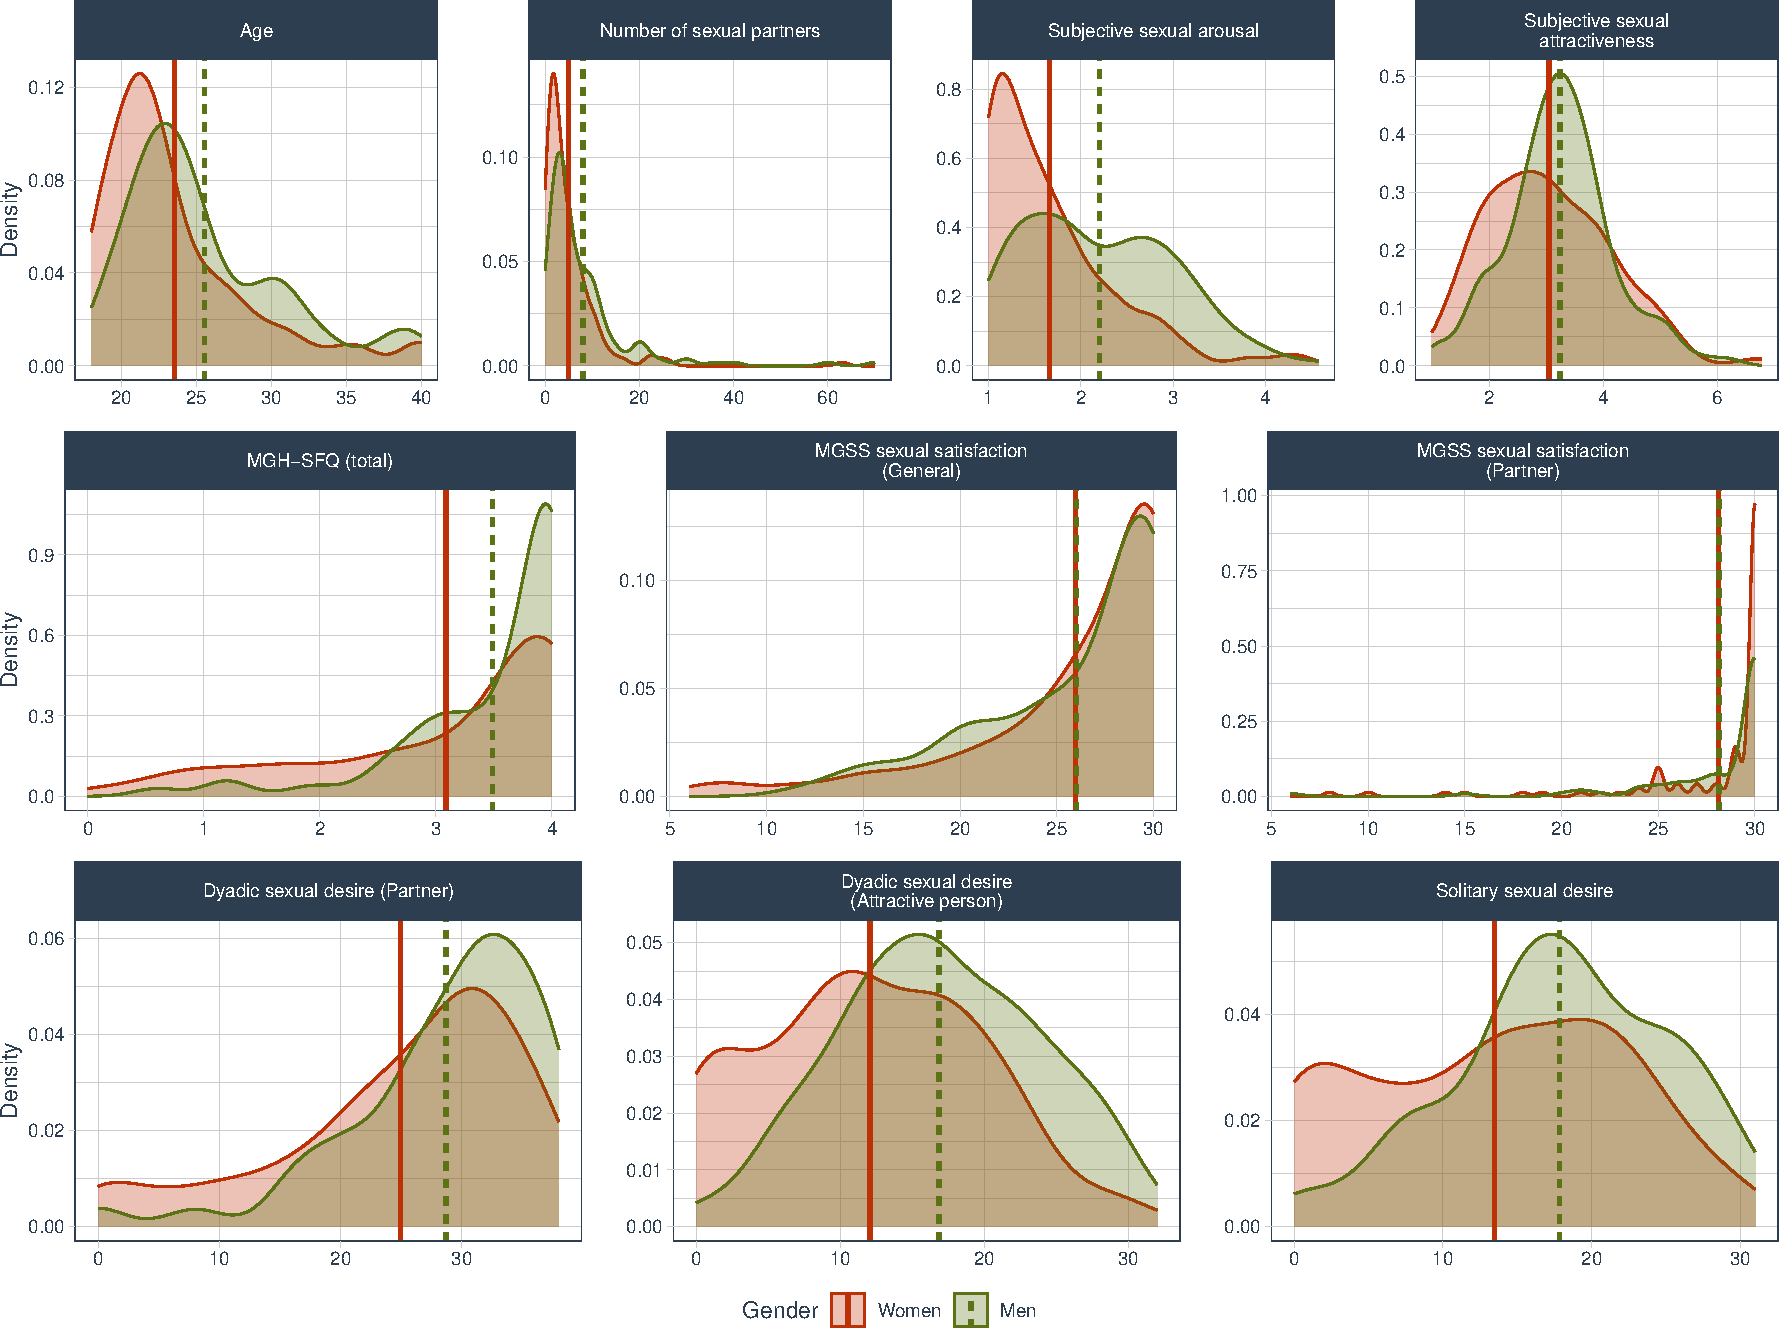
\includegraphics{Deseo_excitacion_sexual_files/figure-latex/density-plot-1.pdf}
\caption{\label{fig:density-plot}Distribution of measured variables by gender. Coloured vertical lines represent mean values by gender. Detailed descriptives are found in Table S1. Because for \emph{Subjective sexual attractiveness} and \emph{Subjective sexual arousal} there are are multiple within-subject observations, densities calculated from mean values per participant.}
\end{figure}

\hypertarget{correlations-between-measured-variables}{%
\subsection{Correlations between measured variables}\label{correlations-between-measured-variables}}

Correlation between numeric variables for women, men, and all participants combined, are reported in Table \ref{tab:corr-tab}.

\hypertarget{table-reftabcorr-tab.-correlations-between-measured-variables}{%
\subsubsection{Table \ref{tab:corr-tab}. Correlations between measured variables}\label{table-reftabcorr-tab.-correlations-between-measured-variables}}

Correlation matrix table.

\begin{Shaded}
\begin{Highlighting}[]
\CommentTok{\# Correlations for women}
\NormalTok{dat.corr.W }\OtherTok{\textless{}{-}}\NormalTok{ dat.desc }\SpecialCharTok{|\textgreater{}}
  \FunctionTok{ungroup}\NormalTok{() }\SpecialCharTok{|\textgreater{}}
  \FunctionTok{filter}\NormalTok{(Gender }\SpecialCharTok{==} \StringTok{"Women"}\NormalTok{) }\SpecialCharTok{|\textgreater{}}
  \FunctionTok{select}\NormalTok{(Age}\SpecialCharTok{:}\StringTok{\textasciigrave{}}\AttributeTok{Dyadic sexual desire (Partner)}\StringTok{\textasciigrave{}}\NormalTok{) }\SpecialCharTok{|\textgreater{}}
  \FunctionTok{corr.stars}\NormalTok{() }\SpecialCharTok{|\textgreater{}}
  \FunctionTok{rownames\_to\_column}\NormalTok{(}\AttributeTok{var =} \StringTok{" "}\NormalTok{)}

\CommentTok{\# Correlations for men}
\NormalTok{dat.corr.M }\OtherTok{\textless{}{-}}\NormalTok{ dat.desc }\SpecialCharTok{|\textgreater{}}
  \FunctionTok{ungroup}\NormalTok{() }\SpecialCharTok{|\textgreater{}}
  \FunctionTok{filter}\NormalTok{(Gender }\SpecialCharTok{==} \StringTok{"Men"}\NormalTok{) }\SpecialCharTok{|\textgreater{}}
  \FunctionTok{select}\NormalTok{(Age}\SpecialCharTok{:}\StringTok{\textasciigrave{}}\AttributeTok{Dyadic sexual desire (Partner)}\StringTok{\textasciigrave{}}\NormalTok{) }\SpecialCharTok{|\textgreater{}}
  \FunctionTok{corr.stars}\NormalTok{() }\SpecialCharTok{|\textgreater{}}
  \FunctionTok{rownames\_to\_column}\NormalTok{(}\AttributeTok{var =} \StringTok{" "}\NormalTok{)}

\CommentTok{\# Correlations for all participants combined}
\NormalTok{dat.corr.All }\OtherTok{\textless{}{-}}\NormalTok{ dat.desc }\SpecialCharTok{|\textgreater{}}
  \FunctionTok{ungroup}\NormalTok{() }\SpecialCharTok{|\textgreater{}}
  \FunctionTok{select}\NormalTok{(Age}\SpecialCharTok{:}\StringTok{\textasciigrave{}}\AttributeTok{Dyadic sexual desire (Partner)}\StringTok{\textasciigrave{}}\NormalTok{) }\SpecialCharTok{|\textgreater{}}
  \FunctionTok{corr.stars}\NormalTok{() }\SpecialCharTok{|\textgreater{}}
  \FunctionTok{rownames\_to\_column}\NormalTok{(}\AttributeTok{var =} \StringTok{" "}\NormalTok{)}

\CommentTok{\# Full formated table}
\FunctionTok{bind\_rows}\NormalTok{(dat.corr.W, dat.corr.M, dat.corr.All) }\SpecialCharTok{|\textgreater{}}
  \FunctionTok{kable}\NormalTok{(}\AttributeTok{digits =} \DecValTok{2}\NormalTok{,}
        \AttributeTok{booktabs =} \ConstantTok{TRUE}\NormalTok{,}
        \AttributeTok{align =} \FunctionTok{c}\NormalTok{(}\StringTok{"l"}\NormalTok{, }\FunctionTok{rep}\NormalTok{(}\StringTok{"c"}\NormalTok{, }\DecValTok{9}\NormalTok{)),}
        \AttributeTok{linesep =} \StringTok{""}\NormalTok{,}
        \AttributeTok{caption =} \StringTok{"Correlations between measured variables"}\NormalTok{,}
        \AttributeTok{escape =} \ConstantTok{FALSE}\NormalTok{) }\SpecialCharTok{|\textgreater{}}
  \FunctionTok{pack\_rows}\NormalTok{(}\AttributeTok{group\_label =} \StringTok{"Women"}\NormalTok{,}
            \AttributeTok{start\_row =} \DecValTok{1}\NormalTok{, }\AttributeTok{end\_row =} \DecValTok{10}\NormalTok{,}
            \AttributeTok{bold =} \ConstantTok{TRUE}\NormalTok{) }\SpecialCharTok{|\textgreater{}}
  \FunctionTok{pack\_rows}\NormalTok{(}\AttributeTok{group\_label =} \StringTok{"Men"}\NormalTok{,}
            \AttributeTok{start\_row =} \DecValTok{11}\NormalTok{, }\AttributeTok{end\_row =} \DecValTok{20}\NormalTok{,}
            \AttributeTok{hline\_before =} \ConstantTok{TRUE}\NormalTok{,}
            \AttributeTok{bold =} \ConstantTok{TRUE}\NormalTok{) }\SpecialCharTok{|\textgreater{}}
  \FunctionTok{pack\_rows}\NormalTok{(}\AttributeTok{group\_label =} \StringTok{"All participants"}\NormalTok{,}
            \AttributeTok{start\_row =} \DecValTok{21}\NormalTok{, }\AttributeTok{end\_row =} \DecValTok{30}\NormalTok{,}
            \AttributeTok{hline\_before =} \ConstantTok{TRUE}\NormalTok{,}
            \AttributeTok{bold =} \ConstantTok{TRUE}\NormalTok{) }\SpecialCharTok{|\textgreater{}}
  \FunctionTok{kable\_styling}\NormalTok{(}\AttributeTok{latex\_options =} \FunctionTok{c}\NormalTok{(}\StringTok{"HOLD\_position"}\NormalTok{, }\StringTok{"scale\_down"}\NormalTok{)) }\SpecialCharTok{|\textgreater{}}
  \FunctionTok{column\_spec}\NormalTok{(}\DecValTok{2}\SpecialCharTok{:}\DecValTok{10}\NormalTok{, }\AttributeTok{width =} \StringTok{"2.2cm"}\NormalTok{) }\SpecialCharTok{|\textgreater{}}
  \FunctionTok{footnote}\NormalTok{(}\AttributeTok{general =} \FunctionTok{paste0}\NormalTok{(}\StringTok{"Values represent Pearson correlation coefficients ($r$). "}\NormalTok{,}
                            \StringTok{"For significance, $\^{}\{}\SpecialCharTok{\textbackslash{}\textbackslash{}\textbackslash{}\textbackslash{}}\StringTok{dagger\}p$ \textless{} 0.1, *$p$ \textless{} 0.05, "}\NormalTok{,}
                            \StringTok{"**$p$ \textless{} 0.01, ***$p$ \textless{} 0.001. "}\NormalTok{,}
                            \StringTok{"Significant correlations are in bold."}\NormalTok{),}
           \AttributeTok{threeparttable =} \ConstantTok{TRUE}\NormalTok{,}
           \AttributeTok{footnote\_as\_chunk =} \ConstantTok{TRUE}\NormalTok{,}
           \AttributeTok{escape =} \ConstantTok{FALSE}\NormalTok{) }\SpecialCharTok{|\textgreater{}}
  \FunctionTok{landscape}\NormalTok{()}
\end{Highlighting}
\end{Shaded}

\begin{landscape}\begin{table}[H]

\caption{\label{tab:corr-tab}Correlations between measured variables}
\centering
\resizebox{\linewidth}{!}{
\begin{threeparttable}
\begin{tabular}[t]{l>{\centering\arraybackslash}p{2.2cm}>{\centering\arraybackslash}p{2.2cm}>{\centering\arraybackslash}p{2.2cm}>{\centering\arraybackslash}p{2.2cm}>{\centering\arraybackslash}p{2.2cm}>{\centering\arraybackslash}p{2.2cm}>{\centering\arraybackslash}p{2.2cm}>{\centering\arraybackslash}p{2.2cm}>{\centering\arraybackslash}p{2.2cm}}
\toprule
  & Age & Number of sexual partners & MGH-SFQ (total) & MGSS sexual satisfaction (General) & MGSS sexual satisfaction (Partner) & Subjective sexual attractiveness & Subjective sexual arousal & Solitary sexual desire & Dyadic sexual desire (Attractive person)\\
\midrule
\addlinespace[0.3em]
\multicolumn{10}{l}{\textbf{Women}}\\
\hspace{1em}Age &  &  &  &  &  &  &  &  \vphantom{2} & \\
\hspace{1em}Number of sexual partners & \textbf{0.24**} &  &  &  &  &  &  &  & \\
\hspace{1em}MGH-SFQ (total) & -0.05 & -0.07 &  &  &  &  &  &  & \\
\hspace{1em}MGSS sexual satisfaction (General) & \textbf{-0.21*} & 0.02 & \textbf{0.46***} &  &  &  &  &  & \\
\hspace{1em}MGSS sexual satisfaction (Partner) & -0.16$^{\dagger}$ & -0.14 & \textbf{0.32***} & \textbf{0.73***} &  &  &  &  & \\
\hspace{1em}Subjective sexual attractiveness & 0.11 & \textbf{0.18*} & -0.04 & \textbf{-0.22*} & -0.18$^{\dagger}$ &  &  &  & \\
\hspace{1em}Subjective sexual arousal & 0.00 & \textbf{0.17*} & -0.13$^{\dagger}$ & -0.18$^{\dagger}$ & -0.16$^{\dagger}$ & \textbf{0.54***} &  &  & \\
\hspace{1em}Solitary sexual desire & -0.14$^{\dagger}$ & \textbf{0.28***} & 0.05 & -0.06 & -0.18$^{\dagger}$ & \textbf{0.31***} & \textbf{0.33***} &  & \\
\hspace{1em}Dyadic sexual desire (Attractive person) & 0.06 & \textbf{0.32***} & \textbf{-0.17*} & -0.04 & -0.17$^{\dagger}$ & \textbf{0.34***} & \textbf{0.36***} & \textbf{0.44***} & \\
\hspace{1em}Dyadic sexual desire (Partner) & 0.00 & \textbf{0.21**} & \textbf{0.43***} & \textbf{0.44***} & \textbf{0.27**} & 0.13$^{\dagger}$ & 0.04 & \textbf{0.31***} & 0.13$^{\dagger}$\\
\addlinespace[0.3em]
\hline
\multicolumn{10}{l}{\textbf{Men}}\\
\hspace{1em}Age &  &  &  &  &  &  &  &  \vphantom{1} & \\
\hspace{1em}Number of sexual partners & \textbf{0.23**} &  &  &  &  &  &  &  & \\
\hspace{1em}MGH-SFQ (total) & 0.04 & 0.02 &  &  &  &  &  &  & \\
\hspace{1em}MGSS sexual satisfaction (General) & \textbf{-0.24*} & -0.08 & \textbf{0.36***} &  &  &  &  &  & \\
\hspace{1em}MGSS sexual satisfaction (Partner) & -0.13 & -0.01 & 0.10 & \textbf{0.63***} &  &  &  &  & \\
\hspace{1em}Subjective sexual attractiveness & 0.10 & -0.05 & -0.08 & -0.10 & -0.02 &  &  &  & \\
\hspace{1em}Subjective sexual arousal & \textbf{0.2*} & 0.07 & 0.05 & -0.14 & -0.09 & \textbf{0.46***} &  &  & \\
\hspace{1em}Solitary sexual desire & -0.16$^{\dagger}$ & 0.00 & 0.09 & 0.10 & 0.17 & \textbf{0.26**} & 0.11 &  & \\
\hspace{1em}Dyadic sexual desire (Attractive person) & 0.12 & \textbf{0.29***} & 0.03 & -0.13 & -0.08 & \textbf{0.25**} & \textbf{0.43***} & \textbf{0.25**} & \\
\hspace{1em}Dyadic sexual desire (Partner) & 0.11 & 0.07 & \textbf{0.36***} & \textbf{0.55***} & \textbf{0.22*} & 0.14 & \textbf{0.24**} & \textbf{0.17*} & \textbf{0.2*}\\
\addlinespace[0.3em]
\hline
\multicolumn{10}{l}{\textbf{All participants}}\\
\hspace{1em}Age &  &  &  &  &  &  &  &  & \\
\hspace{1em}Number of sexual partners & \textbf{0.26***} &  &  &  &  &  &  &  & \\
\hspace{1em}MGH-SFQ (total) & 0.02 & 0.01 &  &  &  &  &  &  & \\
\hspace{1em}MGSS sexual satisfaction (General) & \textbf{-0.22**} & -0.03 & \textbf{0.42***} &  &  &  &  &  & \\
\hspace{1em}MGSS sexual satisfaction (Partner) & \textbf{-0.14*} & -0.07 & \textbf{0.24***} & \textbf{0.69***} &  &  &  &  & \\
\hspace{1em}Subjective sexual attractiveness & \textbf{0.12*} & 0.08 & -0.03 & \textbf{-0.18*} & -0.12 &  &  &  & \\
\hspace{1em}Subjective sexual arousal & \textbf{0.15**} & \textbf{0.17**} & 0.01 & \textbf{-0.15*} & -0.12$^{\dagger}$ & \textbf{0.5***} &  &  & \\
\hspace{1em}Solitary sexual desire & -0.09 & \textbf{0.17**} & 0.11$^{\dagger}$ & 0.00 & -0.05 & \textbf{0.31***} & \textbf{0.3***} &  & \\
\hspace{1em}Dyadic sexual desire (Attractive person) & \textbf{0.14*} & \textbf{0.33***} & -0.04 & -0.07 & -0.12$^{\dagger}$ & \textbf{0.32***} & \textbf{0.45***} & \textbf{0.42***} & \\
\hspace{1em}Dyadic sexual desire (Partner) & 0.08 & \textbf{0.16**} & \textbf{0.43***} & \textbf{0.46***} & \textbf{0.25***} & \textbf{0.15**} & \textbf{0.18**} & \textbf{0.3***} & \textbf{0.21***}\\
\bottomrule
\end{tabular}
\begin{tablenotes}[para]
\item \textit{Note: } 
\item Values represent Pearson correlation coefficients ($r$). For significance, $^{\dagger}p$ < 0.1, *$p$ < 0.05, **$p$ < 0.01, ***$p$ < 0.001. Significant correlations are in bold.
\end{tablenotes}
\end{threeparttable}}
\end{table}
\end{landscape}

\hypertarget{internal-consistency}{%
\subsection{Internal consistency}\label{internal-consistency}}

Six variables were calculated from multiple items (1. MGH-SFQ, 2. Dyadic sexual desire (Partner), 3. Solitary sexual desire, 4. Dyadic sexual desire (Attractive person), 5. MGSS sexual satisfaction (General) and 6. MGSS sexual satisfaction (Partner)).

Data by item, for each participant, is included in the following data base, loaded as \texttt{dat.reli}:

\begin{Shaded}
\begin{Highlighting}[]
\NormalTok{dat.reli }\OtherTok{\textless{}{-}} \FunctionTok{read\_excel}\NormalTok{(}\StringTok{"Data/BD\_ConsistenciaInterna.xlsx"}\NormalTok{)  }\SpecialCharTok{|\textgreater{}}  
  \FunctionTok{mutate}\NormalTok{(}\AttributeTok{Sex =} \FunctionTok{recode\_factor}\NormalTok{(Sex,}
                             \StringTok{"2"} \OtherTok{=} \StringTok{"Women"}\NormalTok{,}
                             \StringTok{"1"} \OtherTok{=} \StringTok{"Men"}\NormalTok{)) }\SpecialCharTok{|\textgreater{}} 
  \FunctionTok{rename}\NormalTok{(}\AttributeTok{Gender =}\NormalTok{ Sex) }\SpecialCharTok{|\textgreater{}} 
  \FunctionTok{filter}\NormalTok{(Participante }\SpecialCharTok{!=} \DecValTok{122}\NormalTok{)}
\end{Highlighting}
\end{Shaded}

Participant 122 was excluded because they did not respond the psychological scales.

To measure the internal consistency of these tests, we used standardized Cronbach's alpha (\(\alpha\) or Tau-equivalent reliability: \(\rho_{T}\)) coefficients, using the function \texttt{cronbach.alpha} from the package \texttt{ltm} (\protect\hyperlink{ref-LtmPackageLatent2006}{Rizopoulos, 2006}).

Importantly, given that for MGH-SFQ one item was answered only by men, the internal consistency of this variable was measured independently for each gender.

\begin{Shaded}
\begin{Highlighting}[]
\CommentTok{\# MGH{-}SFQ for men}
\NormalTok{MGH.m }\OtherTok{\textless{}{-}}\NormalTok{ dat.reli }\SpecialCharTok{|\textgreater{}}
  \FunctionTok{filter}\NormalTok{(Gender }\SpecialCharTok{==} \StringTok{"Men"}\NormalTok{ ) }\SpecialCharTok{|\textgreater{}} 
  \FunctionTok{select}\NormalTok{(}\DecValTok{3}\SpecialCharTok{:}\DecValTok{7}\NormalTok{) }\SpecialCharTok{|\textgreater{}} 
  \FunctionTok{drop\_na}\NormalTok{() }\SpecialCharTok{|\textgreater{}}  
  \FunctionTok{cronbach.alpha}\NormalTok{(}\AttributeTok{CI =} \ConstantTok{TRUE}\NormalTok{, }\AttributeTok{standardized =} \ConstantTok{TRUE}\NormalTok{)}

\CommentTok{\# MGH{-}SFQ for women}
\NormalTok{MGH.w }\OtherTok{\textless{}{-}}\NormalTok{ dat.reli }\SpecialCharTok{|\textgreater{}}
  \FunctionTok{filter}\NormalTok{(Gender }\SpecialCharTok{==} \StringTok{"Women"}\NormalTok{ ) }\SpecialCharTok{|\textgreater{}} 
  \FunctionTok{select}\NormalTok{(}\DecValTok{3}\SpecialCharTok{:}\DecValTok{5}\NormalTok{,}\DecValTok{7}\NormalTok{) }\SpecialCharTok{|\textgreater{}} 
  \FunctionTok{drop\_na}\NormalTok{() }\SpecialCharTok{|\textgreater{}} 
  \FunctionTok{cronbach.alpha}\NormalTok{(}\AttributeTok{CI =} \ConstantTok{TRUE}\NormalTok{, }\AttributeTok{standardized =} \ConstantTok{TRUE}\NormalTok{)}

\CommentTok{\# Dyadic sexual desire (Partner)}
\NormalTok{DSD.p }\OtherTok{\textless{}{-}}\NormalTok{ dat.reli }\SpecialCharTok{|\textgreater{}}
  \FunctionTok{select}\NormalTok{(}\DecValTok{9}\SpecialCharTok{:}\DecValTok{13}\NormalTok{) }\SpecialCharTok{|\textgreater{}} 
  \FunctionTok{drop\_na}\NormalTok{() }\SpecialCharTok{|\textgreater{}} 
  \FunctionTok{cronbach.alpha}\NormalTok{(}\AttributeTok{CI =} \ConstantTok{TRUE}\NormalTok{, }\AttributeTok{standardized =} \ConstantTok{TRUE}\NormalTok{)}

\CommentTok{\# Solitary sexual desire}
\NormalTok{SSD.p }\OtherTok{\textless{}{-}}\NormalTok{ dat.reli }\SpecialCharTok{|\textgreater{}}
  \FunctionTok{select}\NormalTok{(}\DecValTok{15}\SpecialCharTok{:}\DecValTok{18}\NormalTok{) }\SpecialCharTok{|\textgreater{}} 
  \FunctionTok{drop\_na}\NormalTok{() }\SpecialCharTok{|\textgreater{}} 
  \FunctionTok{cronbach.alpha}\NormalTok{(}\AttributeTok{CI =} \ConstantTok{TRUE}\NormalTok{, }\AttributeTok{standardized =} \ConstantTok{TRUE}\NormalTok{)}

\CommentTok{\# Dyadic sexual desire (Attractive person)}
\NormalTok{DSD.a }\OtherTok{\textless{}{-}}\NormalTok{ dat.reli }\SpecialCharTok{|\textgreater{}}
  \FunctionTok{select}\NormalTok{(}\DecValTok{20}\SpecialCharTok{:}\DecValTok{23}\NormalTok{) }\SpecialCharTok{|\textgreater{}} 
  \FunctionTok{drop\_na}\NormalTok{()}\SpecialCharTok{|\textgreater{}} 
  \FunctionTok{cronbach.alpha}\NormalTok{(}\AttributeTok{CI =} \ConstantTok{TRUE}\NormalTok{, }\AttributeTok{standardized =} \ConstantTok{TRUE}\NormalTok{)}

\CommentTok{\# MGSS sexual satisfaction (General)}
\NormalTok{MGSS.g }\OtherTok{\textless{}{-}}\NormalTok{ dat.reli }\SpecialCharTok{|\textgreater{}}
  \FunctionTok{select}\NormalTok{(}\DecValTok{26}\SpecialCharTok{:}\DecValTok{30}\NormalTok{) }\SpecialCharTok{|\textgreater{}} 
  \FunctionTok{drop\_na}\NormalTok{()}\SpecialCharTok{|\textgreater{}} 
  \FunctionTok{cronbach.alpha}\NormalTok{(}\AttributeTok{CI =} \ConstantTok{TRUE}\NormalTok{, }\AttributeTok{standardized =} \ConstantTok{TRUE}\NormalTok{)}

\CommentTok{\# MGSS sexual satisfaction (Partner)}
\NormalTok{MGSS.p }\OtherTok{\textless{}{-}}\NormalTok{ dat.reli }\SpecialCharTok{|\textgreater{}}
  \FunctionTok{select}\NormalTok{(}\DecValTok{32}\SpecialCharTok{:}\DecValTok{36}\NormalTok{) }\SpecialCharTok{|\textgreater{}} 
  \FunctionTok{drop\_na}\NormalTok{()}\SpecialCharTok{|\textgreater{}} 
  \FunctionTok{cronbach.alpha}\NormalTok{(}\AttributeTok{CI =} \ConstantTok{TRUE}\NormalTok{, }\AttributeTok{standardized =} \ConstantTok{TRUE}\NormalTok{)}
\end{Highlighting}
\end{Shaded}

\hypertarget{table-reftabcronbach-tab.-internal-consistency-of-construct-variables}{%
\subsubsection{Table \ref{tab:Cronbach-tab}. Internal consistency of construct variables}\label{table-reftabcronbach-tab.-internal-consistency-of-construct-variables}}

Table of Cronbach's \(\alpha\) for construct variables.

\begin{Shaded}
\begin{Highlighting}[]
\CommentTok{\# Create table}
\FunctionTok{tibble}\NormalTok{(}\AttributeTok{Variable =} \FunctionTok{c}\NormalTok{(}\StringTok{"MGH{-}SFQ"}\NormalTok{, }\StringTok{"MGH{-}SFQ"}\NormalTok{,}
                    \StringTok{"MGSS sexual satisfaction (General)"}\NormalTok{,}
                    \StringTok{"MGSS sexual satisfaction (Partner)"}\NormalTok{,}
                    \StringTok{"Dyadic sexual desire (Partner)"}\NormalTok{, }
                    \StringTok{"Solitary sexual desire"}\NormalTok{, }
                    \StringTok{"Dyadic sexual desire (Attractive person)"}\NormalTok{),}
       \AttributeTok{Gender =} \FunctionTok{c}\NormalTok{(}\StringTok{"Men"}\NormalTok{, }\StringTok{"Women"}\NormalTok{, }\FunctionTok{rep}\NormalTok{(}\StringTok{" "}\NormalTok{, }\DecValTok{5}\NormalTok{)),}
       \AttributeTok{p =} \FunctionTok{c}\NormalTok{(MGH.m}\SpecialCharTok{$}\NormalTok{p,}
\NormalTok{             MGH.w}\SpecialCharTok{$}\NormalTok{p,}
\NormalTok{             MGSS.g}\SpecialCharTok{$}\NormalTok{p,}
\NormalTok{             MGSS.p}\SpecialCharTok{$}\NormalTok{p,}
\NormalTok{             DSD.p}\SpecialCharTok{$}\NormalTok{p,}
\NormalTok{             SSD.p}\SpecialCharTok{$}\NormalTok{p,}
\NormalTok{             DSD.a}\SpecialCharTok{$}\NormalTok{p),}
       \AttributeTok{n =} \FunctionTok{c}\NormalTok{(MGH.m}\SpecialCharTok{$}\NormalTok{n, }
\NormalTok{             MGH.w}\SpecialCharTok{$}\NormalTok{n,}
\NormalTok{             MGSS.g}\SpecialCharTok{$}\NormalTok{n,}
\NormalTok{             MGSS.p}\SpecialCharTok{$}\NormalTok{n,}
\NormalTok{             DSD.p}\SpecialCharTok{$}\NormalTok{n,}
\NormalTok{             SSD.p}\SpecialCharTok{$}\NormalTok{n,}
\NormalTok{             DSD.a}\SpecialCharTok{$}\NormalTok{n),}
       \AttributeTok{alpha =} \FunctionTok{c}\NormalTok{(MGH.m}\SpecialCharTok{$}\NormalTok{alpha,}
\NormalTok{                 MGH.w}\SpecialCharTok{$}\NormalTok{alpha,}
\NormalTok{                 MGSS.g}\SpecialCharTok{$}\NormalTok{alpha,}
\NormalTok{                 MGSS.p}\SpecialCharTok{$}\NormalTok{alpha,}
\NormalTok{                 DSD.p}\SpecialCharTok{$}\NormalTok{alpha,}
\NormalTok{                 SSD.p}\SpecialCharTok{$}\NormalTok{alpha,}
\NormalTok{                 DSD.a}\SpecialCharTok{$}\NormalTok{alpha), }
       \AttributeTok{ci2.5 =} \FunctionTok{c}\NormalTok{(MGH.m}\SpecialCharTok{$}\NormalTok{ci[}\DecValTok{1}\NormalTok{], }
\NormalTok{                 MGH.w}\SpecialCharTok{$}\NormalTok{ci[}\DecValTok{1}\NormalTok{],}
\NormalTok{                 MGSS.g}\SpecialCharTok{$}\NormalTok{ci[}\DecValTok{1}\NormalTok{],}
\NormalTok{                 MGSS.p}\SpecialCharTok{$}\NormalTok{ci[}\DecValTok{1}\NormalTok{],}
\NormalTok{                 DSD.p}\SpecialCharTok{$}\NormalTok{ci[}\DecValTok{1}\NormalTok{],}
\NormalTok{                 SSD.p}\SpecialCharTok{$}\NormalTok{ci[}\DecValTok{1}\NormalTok{],}
\NormalTok{                 DSD.a}\SpecialCharTok{$}\NormalTok{ci[}\DecValTok{1}\NormalTok{]),}
       \AttributeTok{ci97.5 =} \FunctionTok{c}\NormalTok{(MGH.m}\SpecialCharTok{$}\NormalTok{ci[}\DecValTok{2}\NormalTok{], }
\NormalTok{                  MGH.w}\SpecialCharTok{$}\NormalTok{ci[}\DecValTok{2}\NormalTok{],}
\NormalTok{                  MGSS.g}\SpecialCharTok{$}\NormalTok{ci[}\DecValTok{2}\NormalTok{],}
\NormalTok{                  MGSS.p}\SpecialCharTok{$}\NormalTok{ci[}\DecValTok{2}\NormalTok{],}
\NormalTok{                  DSD.p}\SpecialCharTok{$}\NormalTok{ci[}\DecValTok{2}\NormalTok{],}
\NormalTok{                  SSD.p}\SpecialCharTok{$}\NormalTok{ci[}\DecValTok{2}\NormalTok{],}
\NormalTok{                  DSD.a}\SpecialCharTok{$}\NormalTok{ci[}\DecValTok{2}\NormalTok{])) }\SpecialCharTok{|\textgreater{}} 
  \FunctionTok{kable}\NormalTok{(}\AttributeTok{digits =} \DecValTok{2}\NormalTok{,}
        \AttributeTok{booktabs =} \ConstantTok{TRUE}\NormalTok{,}
        \AttributeTok{align =} \FunctionTok{c}\NormalTok{(}\StringTok{"l"}\NormalTok{, }\StringTok{"l"}\NormalTok{, }\FunctionTok{rep}\NormalTok{(}\StringTok{"c"}\NormalTok{, }\DecValTok{5}\NormalTok{)),}
        \AttributeTok{linesep =} \StringTok{""}\NormalTok{,}
        \AttributeTok{caption =} \StringTok{"Internal consistency of measured variables"}\NormalTok{,}
        \AttributeTok{escape =} \ConstantTok{FALSE}\NormalTok{,}
        \AttributeTok{col.names =} \FunctionTok{c}\NormalTok{(}\StringTok{"Variable"}\NormalTok{, }\StringTok{"Gender"}\NormalTok{,}
                      \StringTok{"Items"}\NormalTok{,}
                      \StringTok{"$n$"}\NormalTok{,}
                      \StringTok{"$}\SpecialCharTok{\textbackslash{}\textbackslash{}}\StringTok{alpha$"}\NormalTok{,}
                      \StringTok{"$2.5}\SpecialCharTok{\textbackslash{}\textbackslash{}}\StringTok{\% CI$"}\NormalTok{,}
                      \StringTok{"$97.5}\SpecialCharTok{\textbackslash{}\textbackslash{}}\StringTok{\% CI$"}\NormalTok{)) }\SpecialCharTok{|\textgreater{}}
  \FunctionTok{collapse\_rows}\NormalTok{(}\AttributeTok{columns =} \DecValTok{1}\NormalTok{, }\AttributeTok{valign =} \StringTok{"middle"}\NormalTok{) }\SpecialCharTok{|\textgreater{}}
  \FunctionTok{kable\_styling}\NormalTok{(}\AttributeTok{latex\_options =} \StringTok{"HOLD\_position"}\NormalTok{) }\SpecialCharTok{|\textgreater{}}
  \FunctionTok{footnote}\NormalTok{(}\AttributeTok{general =} \StringTok{"95}\SpecialCharTok{\textbackslash{}\textbackslash{}\textbackslash{}\textbackslash{}}\StringTok{\% confidence intervals were calculated with 1,000 bootstrap samples.}
\StringTok{           Standardized Cronbach\textquotesingle{}s alpha ($}\SpecialCharTok{\textbackslash{}\textbackslash{}\textbackslash{}\textbackslash{}}\StringTok{alpha$) coefficients were computed. }
\StringTok{           MGH{-}SFQ is reported by gender, because one item was answered only by men."}\NormalTok{,}
           \AttributeTok{threeparttable =} \ConstantTok{TRUE}\NormalTok{,}
           \AttributeTok{footnote\_as\_chunk =} \ConstantTok{TRUE}\NormalTok{,}
           \AttributeTok{escape =} \ConstantTok{FALSE}\NormalTok{)}
\end{Highlighting}
\end{Shaded}

\begin{table}[H]

\caption{\label{tab:Cronbach-tab}Internal consistency of measured variables}
\centering
\begin{threeparttable}
\begin{tabular}[t]{llccccc}
\toprule
Variable & Gender & Items & $n$ & $\alpha$ & $2.5\% CI$ & $97.5\% CI$\\
\midrule
 & Men & 5 & 139 & 0.82 & 0.71 & 0.89\\
\cmidrule{2-7}
\multirow{-2}{*}{\raggedright\arraybackslash MGH-SFQ} & Women & 4 & 181 & 0.86 & 0.82 & 0.90\\
\cmidrule{1-7}
MGSS sexual satisfaction (General) &  & 5 & 188 & 0.92 & 0.89 & 0.94\\
\cmidrule{1-7}
MGSS sexual satisfaction (Partner) &  & 5 & 187 & 0.91 & 0.85 & 0.95\\
\cmidrule{1-7}
Dyadic sexual desire (Partner) &  & 5 & 309 & 0.90 & 0.88 & 0.92\\
\cmidrule{1-7}
Solitary sexual desire &  & 4 & 314 & 0.91 & 0.89 & 0.93\\
\cmidrule{1-7}
Dyadic sexual desire (Attractive person) &  & 4 & 320 & 0.89 & 0.87 & 0.91\\
\bottomrule
\end{tabular}
\begin{tablenotes}[para]
\item \textit{Note: } 
\item 95\% confidence intervals were calculated with 1,000 bootstrap samples.
           Standardized Cronbach's alpha ($\alpha$) coefficients were computed. 
           MGH-SFQ is reported by gender, because one item was answered only by men.
\end{tablenotes}
\end{threeparttable}
\end{table}

\hypertarget{hypothesis-tests}{%
\section{Hypothesis tests}\label{hypothesis-tests}}

\hypertarget{hyp1}{%
\subsection{Hypothesis1: Sexual desire by gender, relationship type and sexual desire dimension}\label{hyp1}}

Interaction between relationship type, sexual desire dimension, and gender as predictors of sexual desire. To test this hypothesis, we modeled the effects of Relationship type, Sexual desire dimension, and Gender on the scores of sexual desire.

\hypertarget{filter-data}{%
\subsubsection{Filter data}\label{filter-data}}

Create data frame selecting only relevant variables, and summarizing per sexual desire dimension for each participant (three rows per participant).

\begin{Shaded}
\begin{Highlighting}[]
\NormalTok{dat.comp }\OtherTok{\textless{}{-}}\NormalTok{ dat }\SpecialCharTok{|\textgreater{}}
  \CommentTok{\#mutate(\textasciigrave{}Relationship status\textasciigrave{} = factor(\textasciigrave{}Relationship status\textasciigrave{})) |\textgreater{} }
  \FunctionTok{select}\NormalTok{(Participant, Gender, }
         \CommentTok{\#\textasciigrave{}Stimuli code\textasciigrave{},}
         \StringTok{\textasciigrave{}}\AttributeTok{Solitary sexual desire}\StringTok{\textasciigrave{}}\NormalTok{, }
         \StringTok{\textasciigrave{}}\AttributeTok{Dyadic sexual desire (Attractive person)}\StringTok{\textasciigrave{}}\NormalTok{, }
         \StringTok{\textasciigrave{}}\AttributeTok{Dyadic sexual desire (Partner)}\StringTok{\textasciigrave{}}\NormalTok{, }
\NormalTok{         Relationship,) }\SpecialCharTok{|\textgreater{}}
  \FunctionTok{group\_by}\NormalTok{(Participant, Gender, Relationship) }\SpecialCharTok{|\textgreater{}} 
  \FunctionTok{summarise}\NormalTok{(}\StringTok{\textasciigrave{}}\AttributeTok{Solitary sexual desire}\StringTok{\textasciigrave{}} \OtherTok{=} 
              \FunctionTok{mean}\NormalTok{(}\StringTok{\textasciigrave{}}\AttributeTok{Solitary sexual desire}\StringTok{\textasciigrave{}}\NormalTok{),}
            \StringTok{\textasciigrave{}}\AttributeTok{Dyadic sexual desire (Attractive person)}\StringTok{\textasciigrave{}} \OtherTok{=} 
              \FunctionTok{mean}\NormalTok{(}\StringTok{\textasciigrave{}}\AttributeTok{Dyadic sexual desire (Attractive person)}\StringTok{\textasciigrave{}}\NormalTok{),}
            \StringTok{\textasciigrave{}}\AttributeTok{Dyadic sexual desire (Partner)}\StringTok{\textasciigrave{}} \OtherTok{=} 
              \FunctionTok{mean}\NormalTok{(}\StringTok{\textasciigrave{}}\AttributeTok{Dyadic sexual desire (Partner)}\StringTok{\textasciigrave{}}\NormalTok{)) }\SpecialCharTok{|\textgreater{}} 
  \FunctionTok{pivot\_longer}\NormalTok{(}\AttributeTok{cols =} \StringTok{\textasciigrave{}}\AttributeTok{Solitary sexual desire}\StringTok{\textasciigrave{}}\SpecialCharTok{:}\StringTok{\textasciigrave{}}\AttributeTok{Dyadic sexual desire (Partner)}\StringTok{\textasciigrave{}}\NormalTok{,}
               \AttributeTok{names\_to =} \StringTok{"Dimension"}\NormalTok{, }
               \AttributeTok{values\_to =} \StringTok{"Sexual desire"}\NormalTok{) }\SpecialCharTok{|\textgreater{}} 
  \FunctionTok{mutate}\NormalTok{(}\AttributeTok{Participant =} \FunctionTok{factor}\NormalTok{(Participant)) }\SpecialCharTok{|\textgreater{}}
  \CommentTok{\#mutate("Stimuli code" = factor(\textasciigrave{}Stimuli code\textasciigrave{})) |\textgreater{}}
  \FunctionTok{mutate}\NormalTok{(}\AttributeTok{Dimension =} \FunctionTok{factor}\NormalTok{(Dimension))}
\end{Highlighting}
\end{Shaded}

\hypertarget{fit-model}{%
\subsubsection{Fit model}\label{fit-model}}

We modelled the effects of relationship type, sexual desire dimension, and Gender on the scores of sexual desire as a linear mixed effect model, with random intercepts per participant.

\begin{Shaded}
\begin{Highlighting}[]
\FunctionTok{options}\NormalTok{(}\AttributeTok{contrasts =} \FunctionTok{c}\NormalTok{(}\StringTok{"contr.sum"}\NormalTok{,}\StringTok{"contr.poly"}\NormalTok{))}

\NormalTok{m1 }\OtherTok{\textless{}{-}} \FunctionTok{lmer}\NormalTok{(}\StringTok{\textasciigrave{}}\AttributeTok{Sexual desire}\StringTok{\textasciigrave{}} \SpecialCharTok{\textasciitilde{}}\NormalTok{ Gender }\SpecialCharTok{*}\NormalTok{ Relationship }\SpecialCharTok{*}\NormalTok{ Dimension }\SpecialCharTok{+} 
\NormalTok{            (}\DecValTok{1} \SpecialCharTok{|}\NormalTok{ Participant), }
            \AttributeTok{data =}\NormalTok{ dat.comp)}
\end{Highlighting}
\end{Shaded}

Although it would be ideal to also include random slopes between sexual desire dimensions for each participant, and random intercepts per stimuli (\protect\hyperlink{ref-barr2013}{Barr et al., 2013}; see also \protect\hyperlink{ref-debruine2021}{DeBruine \& Barr, 2021}), this would require to use raw values, instead of averages per participant (i.e.~including the sexual desire rating given to each stimuli). Although this was attempted, such model does not converge.

\hypertarget{model-assumptions}{%
\paragraph{Model assumptions}\label{model-assumptions}}

Most model assumptions were checked using the \texttt{check\_model} function from the \texttt{performance} package (\protect\hyperlink{ref-ludecke2021}{Lüdecke et al., 2021}), and reported in Fig. \ref{fig:assu-m1}. These assumptions do not include collinearity, as the function plots \(VIF\) instead of the recommended Generalized Variance Inflation Factors (\(GVIF\)) and the most comparable \(GVIF^{{1}/{(2 \times df)}}\) (\protect\hyperlink{ref-fox1992}{Fox \& Monette, 1992}). Instead, \(GVIF\) and \(GVIF^{{1}/{(2 \times df)}}\) values are reported in Table \ref{tab:coli-m1}.

\hypertarget{figure-reffigassu-m1.-model-assumptions}{%
\subparagraph{Figure \ref{fig:assu-m1}. Model assumptions}\label{figure-reffigassu-m1.-model-assumptions}}

This figure includes most assumptions: linearity, homogeneity of variance, and normality of both residuals and random effects.

\begin{Shaded}
\begin{Highlighting}[]
\FunctionTok{check\_model}\NormalTok{(m1,}
            \AttributeTok{check =} \FunctionTok{c}\NormalTok{(}\StringTok{"pp\_check"}\NormalTok{,}\StringTok{"linearity"}\NormalTok{, }\StringTok{"homogeneity"}\NormalTok{, }\StringTok{"qq"}\NormalTok{, }\StringTok{"reqq"}\NormalTok{))}
\end{Highlighting}
\end{Shaded}

\begin{figure}
\centering
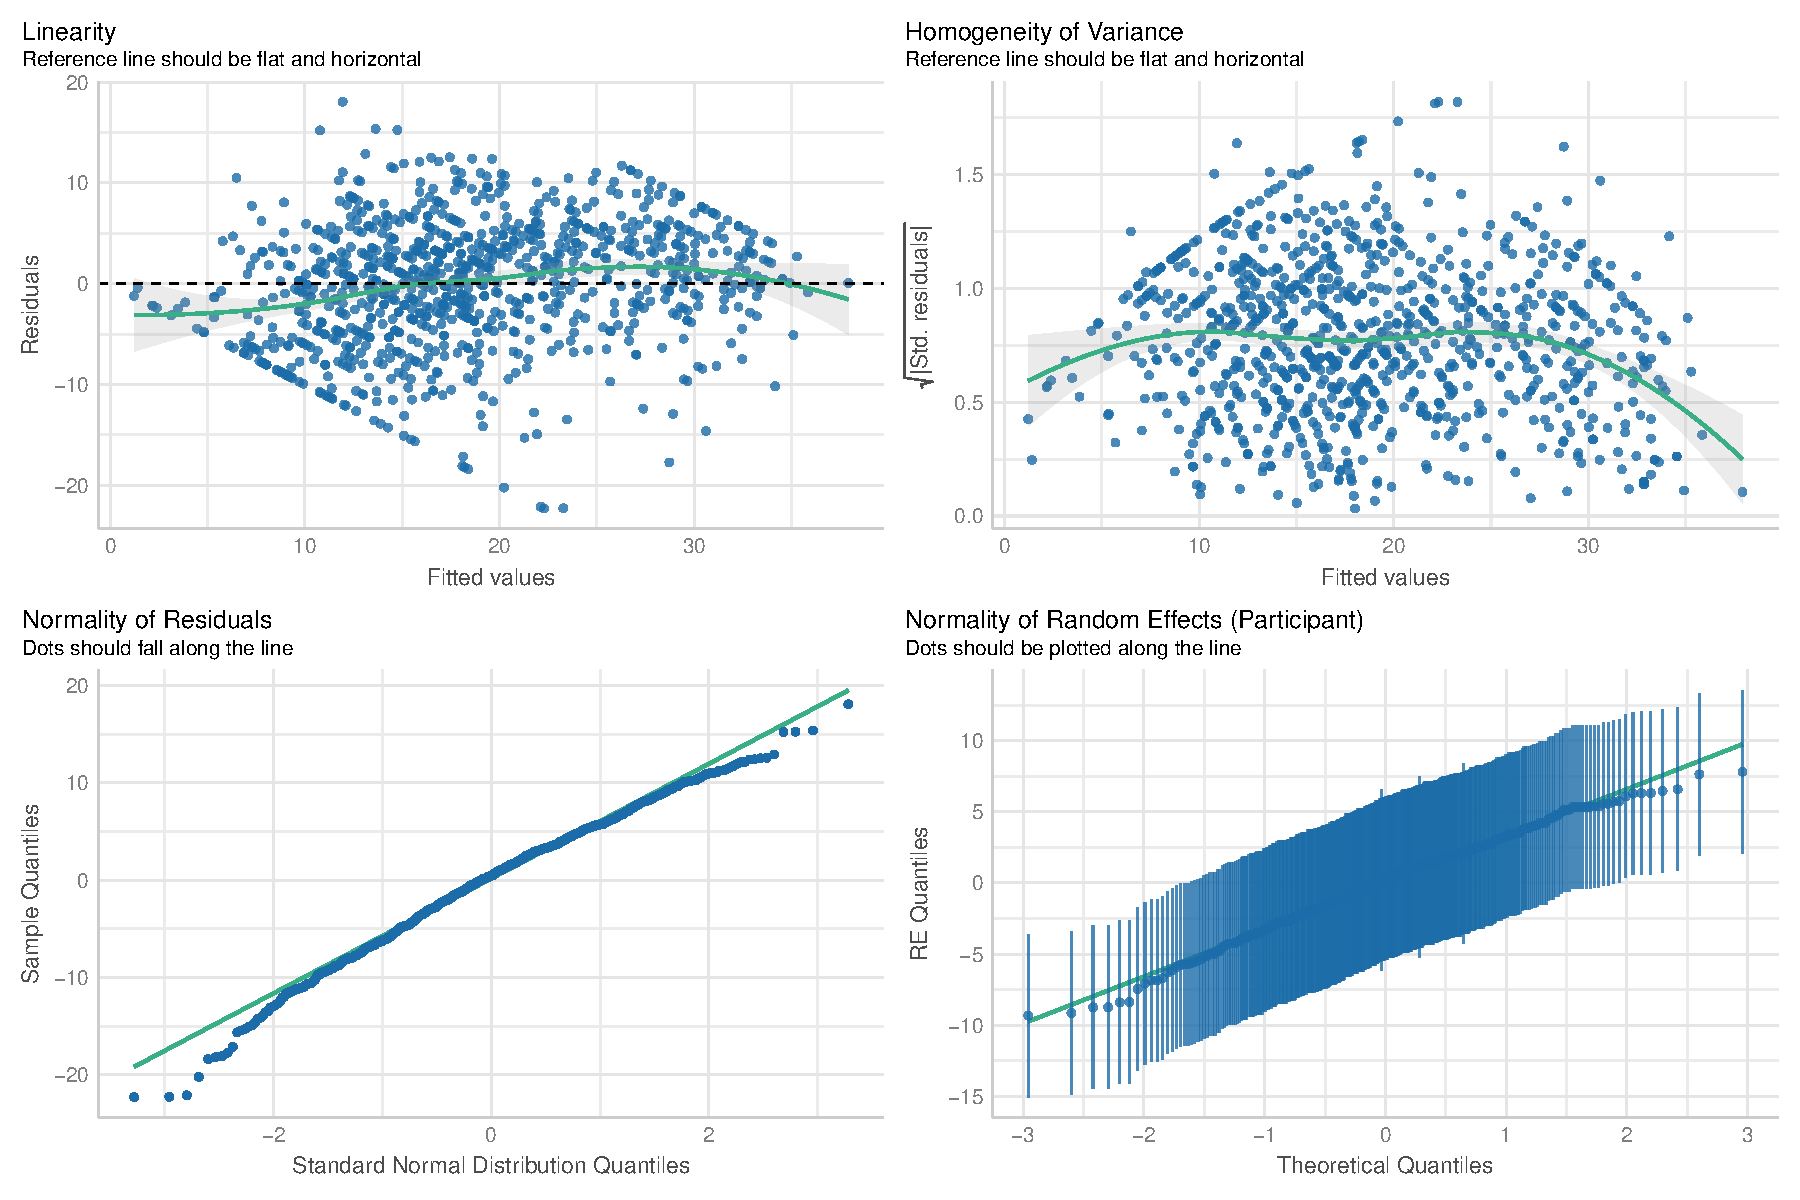
\includegraphics{Deseo_excitacion_sexual_files/figure-latex/assu-m1-1.pdf}
\caption{\label{fig:assu-m1}Model assumptions. Plots represent linearity, homogeneity of variance, and normality of both residuals and random effects (as QQ plots), respectively.}
\end{figure}

\hypertarget{table-reftabcoli-m1.-collinearity}{%
\subparagraph{Table \ref{tab:coli-m1}. Collinearity}\label{table-reftabcoli-m1.-collinearity}}

Given the presence of interactions, that all predictors are categorical, and the absence of random slopes, \(VIF\) and \(GVIF\) values would be expected to be high.

\begin{Shaded}
\begin{Highlighting}[]
\FunctionTok{data.frame}\NormalTok{(}\FunctionTok{vif}\NormalTok{(m1)) }\SpecialCharTok{|\textgreater{}} 
  \FunctionTok{rownames\_to\_column}\NormalTok{() }\SpecialCharTok{|\textgreater{}} 
  \FunctionTok{mutate\_at}\NormalTok{(}\StringTok{"rowname"}\NormalTok{, str\_replace\_all, }\StringTok{":"}\NormalTok{, }\StringTok{" × "}\NormalTok{) }\SpecialCharTok{|\textgreater{}}
  \FunctionTok{mutate\_at}\NormalTok{(}\StringTok{"rowname"}\NormalTok{, str\_replace\_all, }\StringTok{"\textasciigrave{}"}\NormalTok{, }\StringTok{""}\NormalTok{) }\SpecialCharTok{|\textgreater{}} 
  \FunctionTok{kable}\NormalTok{(}\AttributeTok{digits =} \DecValTok{2}\NormalTok{,}
        \AttributeTok{booktabs =} \ConstantTok{TRUE}\NormalTok{,}
        \AttributeTok{align =} \FunctionTok{c}\NormalTok{(}\StringTok{"l"}\NormalTok{, }\FunctionTok{rep}\NormalTok{(}\StringTok{"c"}\NormalTok{, }\DecValTok{3}\NormalTok{)),}
        \AttributeTok{linesep =} \StringTok{""}\NormalTok{,}
        \AttributeTok{caption =} \StringTok{"Variance inflation factors for the model of hypothesis 1b"}\NormalTok{,}
        \AttributeTok{col.names =} \FunctionTok{c}\NormalTok{(}\StringTok{" "}\NormalTok{,}
                      \StringTok{"$GVIF$"}\NormalTok{,}
                      \StringTok{"$df$"}\NormalTok{,}
                      \StringTok{"$GVIF\^{}\{\{1\}/\{(2 }\SpecialCharTok{\textbackslash{}\textbackslash{}}\StringTok{times df)\}\}$"}\NormalTok{),}
        \AttributeTok{escape =} \ConstantTok{FALSE}\NormalTok{) }\SpecialCharTok{|\textgreater{}}
  \FunctionTok{kable\_styling}\NormalTok{(}\AttributeTok{latex\_options =} \StringTok{"HOLD\_position"}\NormalTok{)}
\end{Highlighting}
\end{Shaded}

\begin{table}[H]

\caption{\label{tab:coli-m1}Variance inflation factors for the model of hypothesis 1b}
\centering
\begin{tabular}[t]{lccc}
\toprule
  & $GVIF$ & $df$ & $GVIF^{{1}/{(2 \times df)}}$\\
\midrule
Gender & 1.01 & 1 & 1.00\\
Relationship & 1.02 & 1 & 1.01\\
Dimension & 1.06 & 2 & 1.01\\
Gender × Relationship & 1.02 & 1 & 1.01\\
Gender × Dimension & 1.06 & 2 & 1.01\\
Relationship × Dimension & 1.06 & 2 & 1.01\\
Gender × Relationship × Dimension & 1.06 & 2 & 1.01\\
\bottomrule
\end{tabular}
\end{table}

\hypertarget{table-reftabtab-m1.-regression-type-table-for-the-interaction-between-relationship-type-sexual-desire-dimension-and-gender}{%
\paragraph{\texorpdfstring{Table \ref{tab:tab-m1}. Regression-type table for the interaction between \texttt{Relationship\ type}, \texttt{Sexual\ desire\ dimension}, and \texttt{Gender}}{Table \ref{tab:tab-m1}. Regression-type table for the interaction between Relationship type, Sexual desire dimension, and Gender}}\label{table-reftabtab-m1.-regression-type-table-for-the-interaction-between-relationship-type-sexual-desire-dimension-and-gender}}

This tables summarizes the results of the model.

\begin{Shaded}
\begin{Highlighting}[]
\FunctionTok{summary.sig}\NormalTok{(m1, }\StringTok{"Sexual desire by relationship type, sexual desire dimension and gender"}\NormalTok{)}
\end{Highlighting}
\end{Shaded}

\begin{table}[H]

\caption{\label{tab:tab-m1}Sexual desire by relationship type, sexual desire dimension and gender}
\centering
\resizebox{\linewidth}{!}{
\begin{threeparttable}
\begin{tabular}[t]{lccccc}
\toprule
Effect & Estimate & Std. Error & $df$ & 
                        $t$ & $p$\\
\midrule
(Intercept) & 18.98 & 0.33 & 319.63 & 57.04 & \textbf{< 0.0001}\\
Gender [Women] & -2.13 & 0.33 & 319.63 & -6.40 & \textbf{< 0.0001}\\
Relationship [Stable] & 0.13 & 0.33 & 319.63 & 0.39 & 0.7\\
Dimension [Attractive person DSD] & -4.38 & 0.31 & 636.25 & -14.10 & \textbf{< 0.0001}\\
Dimension [Partner DSD] & 7.54 & 0.31 & 637.61 & 24.19 & \textbf{< 0.0001}\\
Gender [Women] × Relationship [Stable] & -0.44 & 0.33 & 319.63 & -1.31 & 0.19\\
Gender [Women] × Dimension [Attractive person DSD] & -0.16 & 0.31 & 636.25 & -0.51 & 0.61\\
Gender [Women] × Dimension [Partner DSD] & 0.07 & 0.31 & 637.61 & 0.22 & 0.82\\
Relationship [Stable] × Dimension [Attractive person DSD] & -1.35 & 0.31 & 636.25 & -4.34 & \textbf{< 0.0001}\\
Relationship [Stable] × Dimension [Partner DSD] & 2.80 & 0.31 & 637.61 & 8.97 & \textbf{< 0.0001}\\
Gender [Women] × Relationship [Stable] × Dimension [Attractive person DSD] & -0.10 & 0.31 & 636.25 & -0.33 & 0.75\\
Gender [Women] × Relationship [Stable] × Dimension [Partner DSD] & 0.59 & 0.31 & 637.61 & 1.90 & 0.06\\
\bottomrule
\end{tabular}
\begin{tablenotes}[para]
\item \textit{Note: } 
\item $R^2_{conditional}$ = 0.569, $R^2_{marginal}$ = 0.383. Results are from linear mixed models for main 
                              effects and interactions between sexual desire (SD) dimensions,
                              sex, and Stimuli sex.
                              Gender = participants gender (women, men); 
                              Stimuli sex = sex of stimuli (female, male);
                              Attractive person DSD = Dyadic sexual desire toward an 
                              attractive person;
                              Partner DSD = Dyadic sexual desire toward a partner.
                              \textit{Sum-to-zero} contrasts were used to display
                              \textit{p}-values that represent main effects and interactions 
                              in an ANOVA-type manner (i.e. the intercept is the grand mean of 
                              all cells, and estimates are differences between each category
                              mean and the mean of all categories).
                              \textit{Single} was used as reference category
                              for relationship status, \textit{Men} for gender, 
                              and \textit{Solitary} for  sexual desire dimension.
                              Contrasted levels are in square brackets.
                              Significant effects are in bold.
\end{tablenotes}
\end{threeparttable}}
\end{table}

\hypertarget{post-hoc-comparisons}{%
\paragraph{\texorpdfstring{\emph{Post-hoc} comparisons}{Post-hoc comparisons}}\label{post-hoc-comparisons}}

Because only the main effect of (sexual desire) dimension, and the interaction between relationship (type) and dimension are significant, we explored the interaction using estimated marginal means, as well as comparing the relationship types for each of the three sexual desire dimensions.

Table of estimated marginal means and contrasts between sexual desire dimension. All estimated marginal means and contrasts were calculated using the \texttt{emmeans} function from the \texttt{emmeans} package (\protect\hyperlink{ref-emmeanscit}{Lenth, 2022}).

\textcolor{red}{¡¡¡¡AGREGAR COLUMNA DF (EN TODAS LAS TABLAS DE CONTRASTES)!!!!!} \textcolor{green}{\textbf{Hecho!}}

\hypertarget{table-reftabtab-m1a-emms.-estimated-marginal-means-and-contrasts-between-relationship-status-types-for-the-three-dimensions-of-sexual-desire.}{%
\subparagraph{Table \ref{tab:tab-m1a-emms}. Estimated marginal means and contrasts between relationship status types for the three dimensions of sexual desire.}\label{table-reftabtab-m1a-emms.-estimated-marginal-means-and-contrasts-between-relationship-status-types-for-the-three-dimensions-of-sexual-desire.}}

\begin{Shaded}
\begin{Highlighting}[]
\NormalTok{emms.m1a }\OtherTok{\textless{}{-}} \FunctionTok{emmeans}\NormalTok{(m1, }\SpecialCharTok{\textasciitilde{}}\NormalTok{ Dimension,}
                    \AttributeTok{adjust =} \StringTok{"bonferroni"}\NormalTok{,}
                    \AttributeTok{lmer.df =} \StringTok{"satterthwaite"}\NormalTok{)}

\NormalTok{emms.m1a.tab }\OtherTok{\textless{}{-}} \FunctionTok{tibble}\NormalTok{(}\FunctionTok{data.frame}\NormalTok{(emms.m1a)) }\SpecialCharTok{|\textgreater{}}
  \FunctionTok{mutate}\NormalTok{(}\StringTok{"Sexual desire"} \OtherTok{=}\NormalTok{ emmean)}

\NormalTok{t.m1a }\OtherTok{\textless{}{-}} \FunctionTok{contr.stars}\NormalTok{(emms.m1a) }\SpecialCharTok{|\textgreater{}} 
  \FunctionTok{mutate}\NormalTok{(}\AttributeTok{p.value =} \FunctionTok{pval.lev}\NormalTok{(p.value)) }\SpecialCharTok{|\textgreater{}}
  \FunctionTok{mutate}\NormalTok{(}\AttributeTok{group1 =} \FunctionTok{recode\_factor}\NormalTok{(group1,}
                                \StringTok{"Dyadic sexual desire Attractive person"} \OtherTok{=} 
                                  \StringTok{"Dyadic sexual desire (Attractive person)"}\NormalTok{,}
                                \StringTok{"Dyadic sexual desire Partner"} \OtherTok{=} 
                                  \StringTok{"Dyadic sexual desire (Partner)"}\NormalTok{)) }\SpecialCharTok{|\textgreater{}}
  \FunctionTok{mutate}\NormalTok{(}\AttributeTok{group2 =} \FunctionTok{recode\_factor}\NormalTok{(group2,}
                                \StringTok{"Dyadic sexual desire Attractive person"} \OtherTok{=} 
                                  \StringTok{"Dyadic sexual desire (Attractive person)"}\NormalTok{,}
                                \StringTok{"Dyadic sexual desire Partner"} \OtherTok{=} 
                                  \StringTok{"Dyadic sexual desire (Partner)"}\NormalTok{))}

\FunctionTok{merge}\NormalTok{(emms.m1a.tab, t.m1a, }\AttributeTok{by =} \DecValTok{0}\NormalTok{, }\AttributeTok{all =} \ConstantTok{TRUE}\NormalTok{) }\SpecialCharTok{|\textgreater{}}
  \FunctionTok{select}\NormalTok{(}\SpecialCharTok{{-}}\FunctionTok{c}\NormalTok{(}\DecValTok{1}\NormalTok{,}\DecValTok{8}\NormalTok{,}\DecValTok{16}\NormalTok{)) }\SpecialCharTok{|\textgreater{}} 
  \FunctionTok{mutate}\NormalTok{(}\AttributeTok{Dimension =} \FunctionTok{recode\_factor}\NormalTok{(Dimension   ,}
                                \StringTok{"Dyadic sexual desire (Attractive person)"} \OtherTok{=} 
                                  \StringTok{"Dyadic (Attractive person)"}\NormalTok{,}
                                \StringTok{"Dyadic sexual desire (Partner)"} \OtherTok{=} 
                                  \StringTok{"Dyadic (Partner)"}\NormalTok{,}
                                \StringTok{"Solitary sexual desire"} \OtherTok{=} 
                                  \StringTok{"Solitary"}\NormalTok{)) }\SpecialCharTok{|\textgreater{}}
  \FunctionTok{mutate}\NormalTok{(}\AttributeTok{group1 =} \FunctionTok{recode\_factor}\NormalTok{(group1,}
                                \StringTok{"Dyadic sexual desire (Attractive person)"} \OtherTok{=} 
                                  \StringTok{"Dyadic (Attractive person)"}\NormalTok{,}
                                \StringTok{"Dyadic sexual desire (Partner)"} \OtherTok{=} 
                                  \StringTok{"Dyadic (Partner)"}\NormalTok{,}
                                \StringTok{"Solitary sexual desire"} \OtherTok{=} 
                                  \StringTok{"Solitary"}\NormalTok{)) }\SpecialCharTok{|\textgreater{}}
  \FunctionTok{mutate}\NormalTok{(}\AttributeTok{group2 =} \FunctionTok{recode\_factor}\NormalTok{(group2,}
                                \StringTok{"Dyadic sexual desire (Attractive person)"} \OtherTok{=} 
                                  \StringTok{"Dyadic (Attractive person)"}\NormalTok{,}
                                \StringTok{"Dyadic sexual desire (Partner)"} \OtherTok{=} 
                                  \StringTok{"Dyadic (Partner)"}\NormalTok{,}
                                \StringTok{"Solitary sexual desire"} \OtherTok{=} 
                                  \StringTok{"Solitary"}\NormalTok{)) }\SpecialCharTok{|\textgreater{}} 
  \FunctionTok{unite}\NormalTok{(Contrast, group1, group2, }\AttributeTok{sep =} \StringTok{" {-} "}\NormalTok{) }\SpecialCharTok{|\textgreater{}}
  \FunctionTok{mutate\_at}\NormalTok{(}\StringTok{"Contrast"}\NormalTok{, str\_replace\_all, }\StringTok{"NA {-} NA"}\NormalTok{, }\StringTok{" "}\NormalTok{) }\SpecialCharTok{|\textgreater{}} 
  \FunctionTok{kable}\NormalTok{(}\AttributeTok{digits =} \DecValTok{2}\NormalTok{,}
          \AttributeTok{booktabs =} \ConstantTok{TRUE}\NormalTok{,}
          \AttributeTok{align =} \FunctionTok{c}\NormalTok{(}\StringTok{"l"}\NormalTok{, }\FunctionTok{rep}\NormalTok{(}\StringTok{"c"}\NormalTok{, }\DecValTok{5}\NormalTok{), }\StringTok{"l"}\NormalTok{, }\FunctionTok{rep}\NormalTok{(}\StringTok{"c"}\NormalTok{, }\DecValTok{5}\NormalTok{)),}
          \AttributeTok{linesep =} \StringTok{""}\NormalTok{,}
          \AttributeTok{caption =} \StringTok{"Estimated marginal means for the three dimensions of sexual desire"}\NormalTok{,}
          \AttributeTok{col.names =} \FunctionTok{c}\NormalTok{(}\StringTok{"Dimension"}\NormalTok{,}
                        \StringTok{"EMM"}\NormalTok{,}
                        \StringTok{"$SE$"}\NormalTok{,}
                        \StringTok{"$df$"}\NormalTok{,}
                        \StringTok{"$2.5}\SpecialCharTok{\textbackslash{}\textbackslash{}}\StringTok{\% CI$"}\NormalTok{,}
                        \StringTok{"$97.5}\SpecialCharTok{\textbackslash{}\textbackslash{}}\StringTok{\% CI$"}\NormalTok{,}
                        \StringTok{"Contrast"}\NormalTok{,}
                        \StringTok{"Difference"}\NormalTok{,}
                        \StringTok{"$SE$"}\NormalTok{,}
                        \StringTok{"$df$"}\NormalTok{,}
                        \StringTok{"$t$"}\NormalTok{,}
                        \StringTok{"$p$"}\NormalTok{),}
          \AttributeTok{escape =} \ConstantTok{FALSE}\NormalTok{) }\SpecialCharTok{|\textgreater{}}
  \FunctionTok{add\_header\_above}\NormalTok{(}\FunctionTok{c}\NormalTok{(}\StringTok{" "} \OtherTok{=} \DecValTok{6}\NormalTok{, }\StringTok{"Contrasts"} \OtherTok{=} \DecValTok{6}\NormalTok{)) }\SpecialCharTok{|\textgreater{}} 
  \FunctionTok{kable\_styling}\NormalTok{(}\AttributeTok{latex\_options =} \FunctionTok{c}\NormalTok{(}\StringTok{"HOLD\_position"}\NormalTok{, }\StringTok{"scale\_down"}\NormalTok{)) }\SpecialCharTok{|\textgreater{}}
  \FunctionTok{footnote}\NormalTok{(}\AttributeTok{general =} \StringTok{"EMM = estimated marginal mean.}
\StringTok{           Degrees of freedom ($df$) were calculated }
\StringTok{           using the Satterthwaite approximation.}
\StringTok{           Bonferroni adjustment was used."}\NormalTok{,}
           \AttributeTok{threeparttable =} \ConstantTok{TRUE}\NormalTok{,}
           \AttributeTok{footnote\_as\_chunk =} \ConstantTok{TRUE}\NormalTok{,}
           \AttributeTok{escape =} \ConstantTok{FALSE}\NormalTok{)}
\end{Highlighting}
\end{Shaded}

\begin{table}[H]

\caption{\label{tab:tab-m1a-emms}Estimated marginal means for the three dimensions of sexual desire}
\centering
\resizebox{\linewidth}{!}{
\begin{threeparttable}
\begin{tabular}[t]{lccccclccccc}
\toprule
\multicolumn{6}{c}{ } & \multicolumn{6}{c}{Contrasts} \\
\cmidrule(l{3pt}r{3pt}){7-12}
Dimension & EMM & $SE$ & $df$ & $2.5\% CI$ & $97.5\% CI$ & Contrast & Difference & $SE$ & $df$ & $t$ & $p$\\
\midrule
Dyadic (Attractive person) & 14.60 & 0.45 & 808.08 & 13.51 & 15.69 & Dyadic (Attractive person) - Dyadic (Partner) & -11.92 & 0.54 & 637.15 & -22.10 & \textbf{< 0.0001}\\
Dyadic (Partner) & 26.52 & 0.46 & 811.74 & 25.42 & 27.61 & Dyadic (Attractive person) - Solitary & -1.22 & 0.54 & 635.79 & -2.28 & \textbf{0.0232}\\
Solitary & 15.82 & 0.45 & 808.08 & 14.73 & 16.91 & Dyadic (Partner) - Solitary & 10.69 & 0.54 & 637.15 & 19.83 & \textbf{< 0.0001}\\
\bottomrule
\end{tabular}
\begin{tablenotes}[para]
\item \textit{Note: } 
\item EMM = estimated marginal mean.
           Degrees of freedom ($df$) were calculated 
           using the Satterthwaite approximation.
           Bonferroni adjustment was used.
\end{tablenotes}
\end{threeparttable}}
\end{table}

\hypertarget{table-reftabtab-m1b-emms.-estimated-marginal-means-and-contrasts-between-relationship-status-types-for-the-three-dimensions-of-sexual-desire}{%
\subparagraph{Table \ref{tab:tab-m1b-emms}. Estimated marginal means and contrasts between relationship status types for the three dimensions of sexual desire}\label{table-reftabtab-m1b-emms.-estimated-marginal-means-and-contrasts-between-relationship-status-types-for-the-three-dimensions-of-sexual-desire}}

Table of estimated marginal means and contrasts between relationship status for each sexual desire dimension. All estimated marginal means and contrasts were calculated using the \texttt{emmeans} function from the \texttt{emmeans} package (\protect\hyperlink{ref-emmeanscit}{Lenth, 2022}).

\begin{Shaded}
\begin{Highlighting}[]
\NormalTok{emms.m1b }\OtherTok{\textless{}{-}} \FunctionTok{emmeans}\NormalTok{(m1, }\SpecialCharTok{\textasciitilde{}}\NormalTok{ Relationship }\SpecialCharTok{|}\NormalTok{ Dimension,}
                    \AttributeTok{adjust =} \StringTok{"bonferroni"}\NormalTok{,}
                    \AttributeTok{lmer.df =} \StringTok{"satterthwaite"}\NormalTok{)}

\NormalTok{emms.m1b.tab }\OtherTok{\textless{}{-}} \FunctionTok{tibble}\NormalTok{(}\FunctionTok{data.frame}\NormalTok{(emms.m1b)) }\SpecialCharTok{|\textgreater{}}
  \FunctionTok{mutate}\NormalTok{(}\StringTok{"Sexual desire"} \OtherTok{=}\NormalTok{ emmean)}

\NormalTok{t.m1b }\OtherTok{\textless{}{-}} \FunctionTok{contr.stars}\NormalTok{(emms.m1b) }\SpecialCharTok{|\textgreater{}} 
  \FunctionTok{mutate}\NormalTok{(}\AttributeTok{p.value =} \FunctionTok{pval.lev}\NormalTok{(p.value))}

\NormalTok{t.m1b.f }\OtherTok{\textless{}{-}}\NormalTok{ t.m1b }\SpecialCharTok{|\textgreater{}} 
  \FunctionTok{insertRows}\NormalTok{(}\DecValTok{2}\NormalTok{, }\AttributeTok{new =} \ConstantTok{NA}\NormalTok{) }\SpecialCharTok{|\textgreater{}}
  \FunctionTok{insertRows}\NormalTok{(}\DecValTok{4}\NormalTok{, }\AttributeTok{new =} \ConstantTok{NA}\NormalTok{)}

\FunctionTok{merge}\NormalTok{(emms.m1b.tab, t.m1b.f, }\AttributeTok{by =} \DecValTok{0}\NormalTok{, }\AttributeTok{all =} \ConstantTok{TRUE}\NormalTok{) }\SpecialCharTok{|\textgreater{}}
  \FunctionTok{select}\NormalTok{(}\SpecialCharTok{{-}}\FunctionTok{c}\NormalTok{(}\DecValTok{1}\NormalTok{,}\DecValTok{3}\NormalTok{,}\DecValTok{9}\NormalTok{,}\DecValTok{12}\NormalTok{,}\DecValTok{18}\NormalTok{)) }\SpecialCharTok{|\textgreater{}} 
  \FunctionTok{unite}\NormalTok{(Contrast, group1, group2, }\AttributeTok{sep =} \StringTok{" {-} "}\NormalTok{) }\SpecialCharTok{|\textgreater{}}
  \FunctionTok{mutate\_at}\NormalTok{(}\StringTok{"Contrast"}\NormalTok{, str\_replace\_all, }\StringTok{"NA {-} NA"}\NormalTok{, }\StringTok{" "}\NormalTok{) }\SpecialCharTok{|\textgreater{}} 
  \FunctionTok{kable}\NormalTok{(}\AttributeTok{digits =} \DecValTok{2}\NormalTok{,}
          \AttributeTok{booktabs =} \ConstantTok{TRUE}\NormalTok{,}
          \AttributeTok{align =} \FunctionTok{c}\NormalTok{(}\StringTok{"l"}\NormalTok{, }\FunctionTok{rep}\NormalTok{(}\StringTok{"c"}\NormalTok{, }\DecValTok{5}\NormalTok{), }\StringTok{"l"}\NormalTok{, }\FunctionTok{rep}\NormalTok{(}\StringTok{"c"}\NormalTok{, }\DecValTok{5}\NormalTok{)),}
          \AttributeTok{linesep =} \StringTok{""}\NormalTok{,}
          \AttributeTok{caption =} \StringTok{"Estimated marginal means for the three dimensions of sexual desire by}
\StringTok{        relationship status"}\NormalTok{,}
          \AttributeTok{col.names =} \FunctionTok{c}\NormalTok{(}\StringTok{"Relationship"}\NormalTok{,}
                        \StringTok{"EMM"}\NormalTok{,}
                        \StringTok{"$SE$"}\NormalTok{,}
                        \StringTok{"$df$"}\NormalTok{,}
                        \StringTok{"$2.5}\SpecialCharTok{\textbackslash{}\textbackslash{}}\StringTok{\% CI$"}\NormalTok{,}
                        \StringTok{"$97.5}\SpecialCharTok{\textbackslash{}\textbackslash{}}\StringTok{\% CI$"}\NormalTok{,}
                        \StringTok{"Contrast"}\NormalTok{,}
                        \StringTok{"Difference"}\NormalTok{,}
                        \StringTok{"$SE$"}\NormalTok{,}
                        \StringTok{"$df$"}\NormalTok{,}
                        \StringTok{"$t$"}\NormalTok{,}
                        \StringTok{"$p$"}\NormalTok{),}
          \AttributeTok{escape =} \ConstantTok{FALSE}\NormalTok{) }\SpecialCharTok{|\textgreater{}}
  \FunctionTok{pack\_rows}\NormalTok{(}\AttributeTok{group\_label =} \StringTok{"Dyadic sexual desire (Attractive person)"}\NormalTok{,}
            \AttributeTok{start\_row =} \DecValTok{1}\NormalTok{,}
            \AttributeTok{end\_row =} \DecValTok{2}\NormalTok{,}
            \AttributeTok{bold =} \ConstantTok{TRUE}\NormalTok{) }\SpecialCharTok{|\textgreater{}}
  \FunctionTok{pack\_rows}\NormalTok{(}\AttributeTok{group\_label =} \StringTok{"Dyadic sexual desire (Partner)"}\NormalTok{,}
            \AttributeTok{start\_row =} \DecValTok{3}\NormalTok{,}
            \AttributeTok{end\_row =} \DecValTok{4}\NormalTok{,}
            \AttributeTok{hline\_before =} \ConstantTok{TRUE}\NormalTok{,}
            \AttributeTok{bold =} \ConstantTok{TRUE}\NormalTok{) }\SpecialCharTok{|\textgreater{}}
  \FunctionTok{pack\_rows}\NormalTok{(}\AttributeTok{group\_label =} \StringTok{"Solitary sexual desire"}\NormalTok{,}
            \AttributeTok{start\_row =} \DecValTok{5}\NormalTok{,}
            \AttributeTok{end\_row =} \DecValTok{6}\NormalTok{,}
            \AttributeTok{hline\_before =} \ConstantTok{TRUE}\NormalTok{,}
            \AttributeTok{bold =} \ConstantTok{TRUE}\NormalTok{) }\SpecialCharTok{|\textgreater{}}
  \FunctionTok{add\_header\_above}\NormalTok{(}\FunctionTok{c}\NormalTok{(}\StringTok{" "} \OtherTok{=} \DecValTok{6}\NormalTok{, }\StringTok{"Contrasts"} \OtherTok{=} \DecValTok{6}\NormalTok{)) }\SpecialCharTok{|\textgreater{}} 
  \FunctionTok{kable\_styling}\NormalTok{(}\AttributeTok{latex\_options =} \FunctionTok{c}\NormalTok{(}\StringTok{"HOLD\_position"}\NormalTok{, }\StringTok{"scale\_down"}\NormalTok{)) }\SpecialCharTok{|\textgreater{}}
  \FunctionTok{footnote}\NormalTok{(}\AttributeTok{general =} \StringTok{"EMM = estimated marginal mean.}
\StringTok{           Degrees of freedom ($df$) were calculated }
\StringTok{           using the Satterthwaite approximation.}
\StringTok{           Bonferroni adjustment was used."}\NormalTok{,}
           \AttributeTok{threeparttable =} \ConstantTok{TRUE}\NormalTok{,}
           \AttributeTok{footnote\_as\_chunk =} \ConstantTok{TRUE}\NormalTok{,}
           \AttributeTok{escape =} \ConstantTok{FALSE}\NormalTok{)}
\end{Highlighting}
\end{Shaded}

\begin{table}[H]

\caption{\label{tab:tab-m1b-emms}Estimated marginal means for the three dimensions of sexual desire by
        relationship status}
\centering
\resizebox{\linewidth}{!}{
\begin{threeparttable}
\begin{tabular}[t]{lccccclccccc}
\toprule
\multicolumn{6}{c}{ } & \multicolumn{6}{c}{Contrasts} \\
\cmidrule(l{3pt}r{3pt}){7-12}
Relationship & EMM & $SE$ & $df$ & $2.5\% CI$ & $97.5\% CI$ & Contrast & Difference & $SE$ & $df$ & $t$ & $p$\\
\midrule
\addlinespace[0.3em]
\multicolumn{12}{l}{\textbf{Dyadic sexual desire (Attractive person)}}\\
\hspace{1em}Stable & 13.38 & 0.62 & 808.08 & 12.00 & 14.76 & Stable - Single & -2.43 & 0.91 & 808.08 & -2.68 & \textbf{0.0076}\\
\hspace{1em}Single & 15.82 & 0.67 & 808.08 & 14.31 & 17.32 &  &  &  &  &  & \\
\addlinespace[0.3em]
\hline
\multicolumn{12}{l}{\textbf{Dyadic sexual desire (Partner)}}\\
\hspace{1em}Stable & 29.44 & 0.62 & 808.08 & 28.06 & 30.82 & Stable - Single & 5.85 & 0.91 & 811.74 & 6.41 & \textbf{< 0.0001}\\
\hspace{1em}Single & 23.59 & 0.67 & 814.77 & 22.08 & 25.10 &  &  &  &  &  & \\
\addlinespace[0.3em]
\hline
\multicolumn{12}{l}{\textbf{Solitary sexual desire}}\\
\hspace{1em}Stable & 14.50 & 0.62 & 808.08 & 13.12 & 15.89 & Stable - Single & -2.64 & 0.91 & 808.08 & -2.90 & \textbf{0.0038}\\
\hspace{1em}Single & 17.14 & 0.67 & 808.08 & 15.64 & 18.64 &  &  &  &  &  & \\
\bottomrule
\end{tabular}
\begin{tablenotes}[para]
\item \textit{Note: } 
\item EMM = estimated marginal mean.
           Degrees of freedom ($df$) were calculated 
           using the Satterthwaite approximation.
           Bonferroni adjustment was used.
\end{tablenotes}
\end{threeparttable}}
\end{table}

\hypertarget{figure-reffigfig-h1.-differences-among-the-three-dimensions-of-sexual-desire}{%
\subsubsection{Figure \ref{fig:fig-h1}. Differences among the three dimensions of sexual desire}\label{figure-reffigfig-h1.-differences-among-the-three-dimensions-of-sexual-desire}}

This figure summarizes the results of hypothesis 1.

\begin{Shaded}
\begin{Highlighting}[]
\CommentTok{\# Figure Dimension main effect}
\NormalTok{h1a }\OtherTok{\textless{}{-}} \FunctionTok{ggplot}\NormalTok{(dat.comp, }\FunctionTok{aes}\NormalTok{(}\AttributeTok{x =}\NormalTok{ Dimension, }\AttributeTok{y =} \StringTok{\textasciigrave{}}\AttributeTok{Sexual desire}\StringTok{\textasciigrave{}}\NormalTok{, }\AttributeTok{color =}\NormalTok{ Dimension)) }\SpecialCharTok{+}
  \FunctionTok{geom\_violin}\NormalTok{() }\SpecialCharTok{+}
  \FunctionTok{geom\_jitter}\NormalTok{(}\AttributeTok{alpha =} \FloatTok{0.3}\NormalTok{, }\AttributeTok{width =} \FloatTok{0.1}\NormalTok{) }\SpecialCharTok{+}
  \FunctionTok{scale\_color\_manual}\NormalTok{(}\AttributeTok{values =}\NormalTok{ color.Dimension) }\SpecialCharTok{+}
  \FunctionTok{scale\_fill\_manual}\NormalTok{(}\AttributeTok{values =}\NormalTok{ color.Dimension) }\SpecialCharTok{+}
  \FunctionTok{geom\_errorbar}\NormalTok{(}\AttributeTok{data =}\NormalTok{ emms.m1a.tab, }
                \AttributeTok{mapping =} \FunctionTok{aes}\NormalTok{(}\AttributeTok{ymin =}\NormalTok{ lower.CL, }\AttributeTok{ymax =}\NormalTok{ upper.CL), }
                \AttributeTok{colour =} \StringTok{"black"}\NormalTok{, }\AttributeTok{width =} \FloatTok{0.1}\NormalTok{) }\SpecialCharTok{+}
  \FunctionTok{geom\_point}\NormalTok{(}\AttributeTok{data =}\NormalTok{ emms.m1a.tab, }
             \AttributeTok{position =} \FunctionTok{position\_dodge}\NormalTok{(}\FloatTok{0.1}\NormalTok{), }
             \AttributeTok{shape =} \DecValTok{21}\NormalTok{, }\AttributeTok{size =} \DecValTok{3}\NormalTok{,}
             \AttributeTok{color =} \StringTok{"black"}\NormalTok{, }\AttributeTok{fill =} \StringTok{"white"}\NormalTok{) }\SpecialCharTok{+}
  \FunctionTok{stat\_pvalue\_manual}\NormalTok{(t.m1a, }
                     \AttributeTok{label =} \StringTok{"p.signif"}\NormalTok{, }
                     \AttributeTok{y.position =} \FunctionTok{c}\NormalTok{(}\DecValTok{44}\NormalTok{, }\DecValTok{47}\NormalTok{, }\DecValTok{41}\NormalTok{), }
                     \AttributeTok{tip.length =} \DecValTok{0}\NormalTok{) }\SpecialCharTok{+}
  \FunctionTok{theme\_tq}\NormalTok{()}

\CommentTok{\# Figure Relationship × Dimension interaction}
\NormalTok{h1b }\OtherTok{\textless{}{-}} \FunctionTok{ggplot}\NormalTok{(dat.comp, }\FunctionTok{aes}\NormalTok{(}\AttributeTok{x =}\NormalTok{ Relationship, }\AttributeTok{y =} \StringTok{\textasciigrave{}}\AttributeTok{Sexual desire}\StringTok{\textasciigrave{}}\NormalTok{, }\AttributeTok{color =}\NormalTok{ Relationship)) }\SpecialCharTok{+}
  \FunctionTok{geom\_violin}\NormalTok{() }\SpecialCharTok{+}
  \FunctionTok{geom\_jitter}\NormalTok{(}\AttributeTok{alpha =} \FloatTok{0.3}\NormalTok{, }\AttributeTok{width =} \FloatTok{0.1}\NormalTok{) }\SpecialCharTok{+}
  \FunctionTok{scale\_color\_manual}\NormalTok{(}\AttributeTok{values =}\NormalTok{ color.Relationship) }\SpecialCharTok{+}
  \FunctionTok{scale\_fill\_manual}\NormalTok{(}\AttributeTok{values =}\NormalTok{ color.Relationship) }\SpecialCharTok{+}
  \FunctionTok{facet\_wrap}\NormalTok{(}\SpecialCharTok{\textasciitilde{}}\NormalTok{Dimension) }\SpecialCharTok{+}
  \FunctionTok{geom\_errorbar}\NormalTok{(}\AttributeTok{data =}\NormalTok{ emms.m1b.tab, }
                \AttributeTok{mapping =} \FunctionTok{aes}\NormalTok{(}\AttributeTok{ymin =}\NormalTok{ lower.CL, }\AttributeTok{ymax =}\NormalTok{ upper.CL), }
                \AttributeTok{colour =} \StringTok{"black"}\NormalTok{, }\AttributeTok{width =} \FloatTok{0.1}\NormalTok{) }\SpecialCharTok{+}
  \FunctionTok{geom\_point}\NormalTok{(}\AttributeTok{data =}\NormalTok{ emms.m1b.tab, }
             \AttributeTok{position =} \FunctionTok{position\_dodge}\NormalTok{(}\FloatTok{0.1}\NormalTok{), }
             \AttributeTok{shape =} \DecValTok{21}\NormalTok{, }\AttributeTok{size =} \DecValTok{3}\NormalTok{,}
             \AttributeTok{color =} \StringTok{"black"}\NormalTok{, }\AttributeTok{fill =} \StringTok{"white"}\NormalTok{) }\SpecialCharTok{+}
  \FunctionTok{stat\_pvalue\_manual}\NormalTok{(t.m1b, }
                     \AttributeTok{label =} \StringTok{"p.signif"}\NormalTok{, }
                     \AttributeTok{y.position =} \FunctionTok{c}\NormalTok{(}\DecValTok{34}\NormalTok{, }\DecValTok{40}\NormalTok{, }\DecValTok{33}\NormalTok{), }
                     \AttributeTok{tip.length =} \DecValTok{0}\NormalTok{) }\SpecialCharTok{+}
  \FunctionTok{theme\_tq}\NormalTok{()}

\CommentTok{\# Full figure for hypothesis 1 (a and b)}
\NormalTok{p1f }\OtherTok{\textless{}{-}} \FunctionTok{ggarrange}\NormalTok{(h1a, h1b,}
                 \AttributeTok{labels =} \StringTok{"auto"}\NormalTok{,}
                 \AttributeTok{legend =} \StringTok{"bottom"}\NormalTok{,}
                 \AttributeTok{nrow =} \DecValTok{2}\NormalTok{)}
\NormalTok{p1f}
\end{Highlighting}
\end{Shaded}

\begin{figure}
\centering
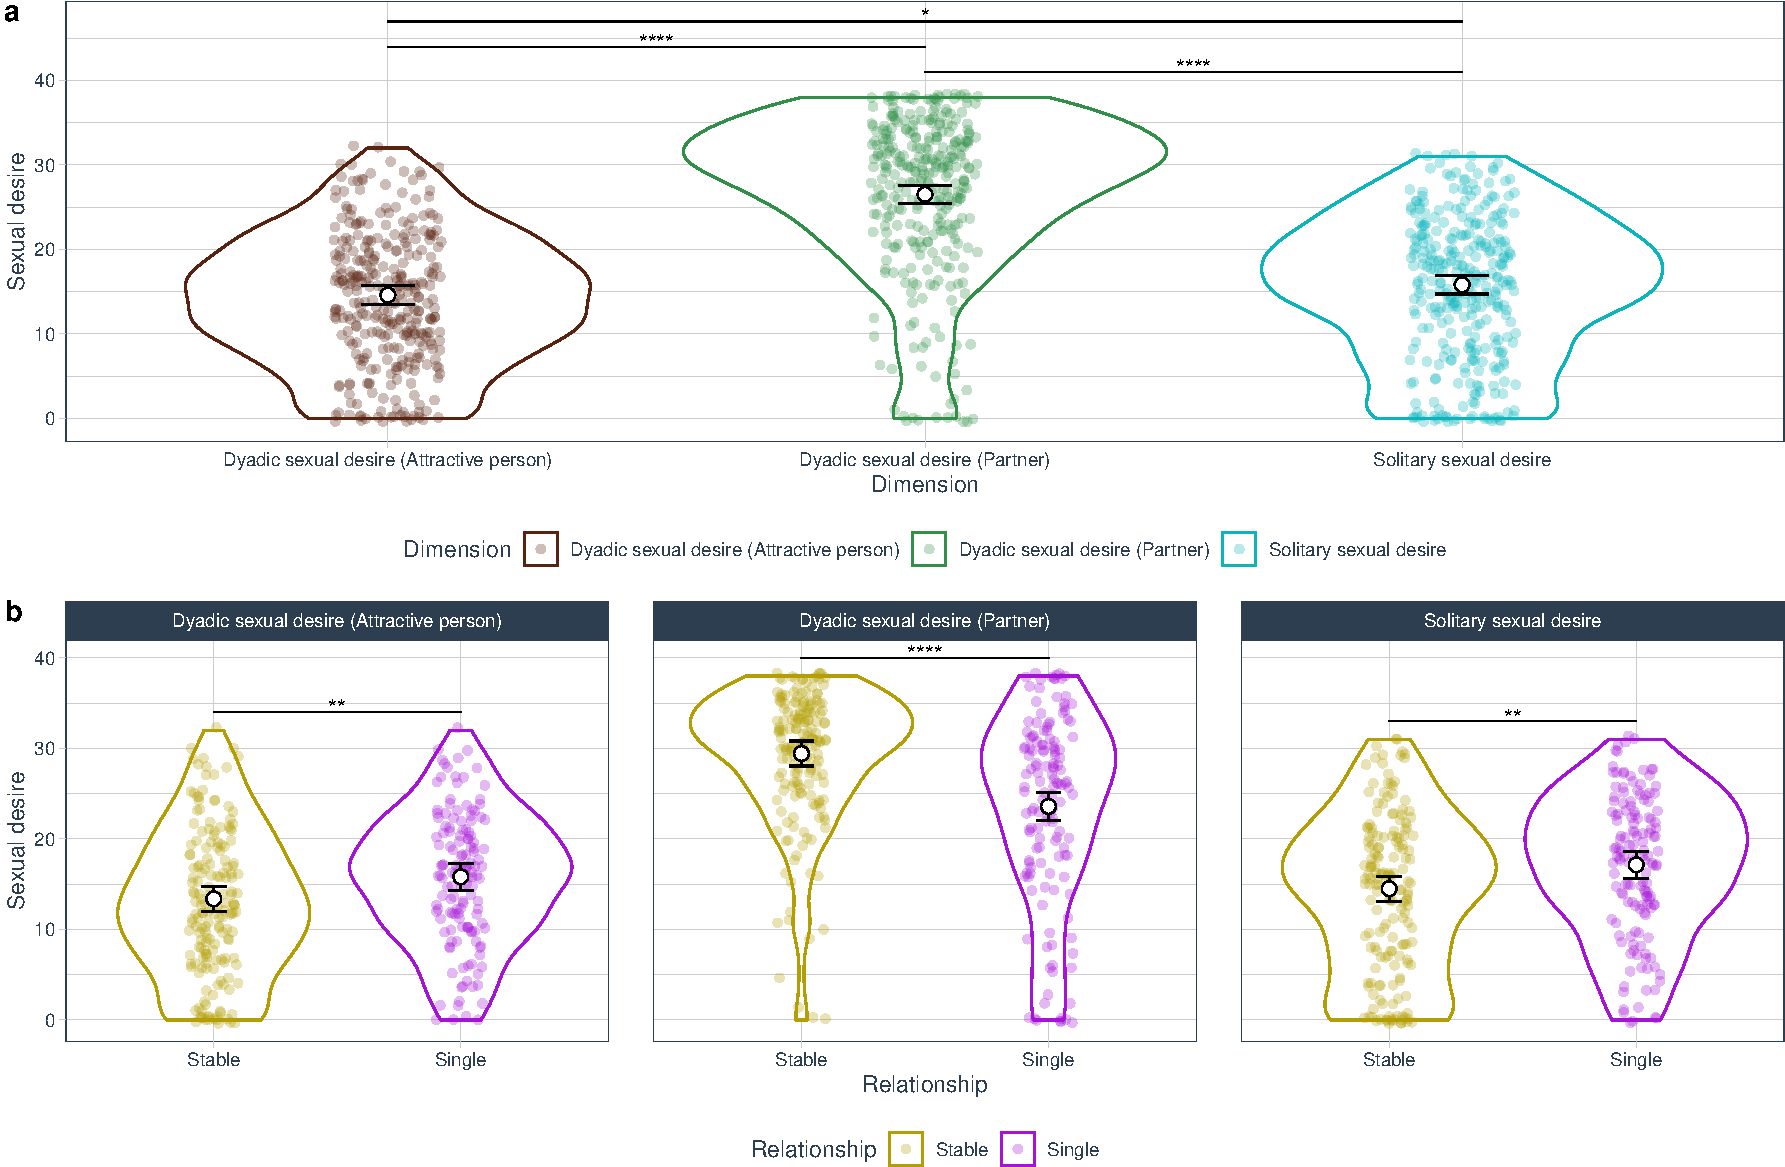
\includegraphics{Deseo_excitacion_sexual_files/figure-latex/fig-h1-1.pdf}
\caption{\label{fig:fig-h1}Differences among the three dimensions of sexual desire (Solitary sexual desire, Dyadic sexual desire (Partner), dyadic sexual desire (Attractive person)). \textbf{(a)} Simple comparison between dimensions of sexual desire (for detailed results, see Table \ref{tab:tab-m1a-emms}); \textbf{(b)} Interaction between relationship type and sexual desire dimension (see Table \ref{tab:tab-m1}; for detailed results, see Table \ref{tab:tab-m1b-emms}). White dots and black bars represent estimated marginal means and 95\% CI. In all cases, significant effects are represented with lines and stars: *\emph{p} \textless{} 0.05, **\emph{p} \textless{} 0.01, ***\emph{p} \textless{} 0.001, ****\emph{p} \textless{} 0.0001.}
\end{figure}

\hypertarget{hypothesis2}{%
\subsection{Hypothesis 2}\label{hypothesis2}}

Data

\begin{Shaded}
\begin{Highlighting}[]
\NormalTok{dat.fin }\OtherTok{\textless{}{-}}\NormalTok{ dat }\SpecialCharTok{|\textgreater{}}
  \FunctionTok{mutate}\NormalTok{(}\StringTok{\textasciigrave{}}\AttributeTok{Solitary sexual desire (C)}\StringTok{\textasciigrave{}} \OtherTok{=} 
           \FunctionTok{scale}\NormalTok{(}\StringTok{\textasciigrave{}}\AttributeTok{Solitary sexual desire}\StringTok{\textasciigrave{}}\NormalTok{,}
                 \AttributeTok{center =} \ConstantTok{TRUE}\NormalTok{, }\AttributeTok{scale =} \ConstantTok{FALSE}\NormalTok{)) }\SpecialCharTok{|\textgreater{}}
  \FunctionTok{mutate}\NormalTok{(}\StringTok{\textasciigrave{}}\AttributeTok{Dyadic sexual desire (Attractive person) (C)}\StringTok{\textasciigrave{}} \OtherTok{=} 
           \FunctionTok{scale}\NormalTok{(}\StringTok{\textasciigrave{}}\AttributeTok{Dyadic sexual desire (Attractive person)}\StringTok{\textasciigrave{}}\NormalTok{, }
                 \AttributeTok{center =} \ConstantTok{TRUE}\NormalTok{, }\AttributeTok{scale =} \ConstantTok{FALSE}\NormalTok{)) }\SpecialCharTok{|\textgreater{}}
  \FunctionTok{mutate}\NormalTok{(}\StringTok{\textasciigrave{}}\AttributeTok{Dyadic sexual desire (Partner) (C)}\StringTok{\textasciigrave{}} \OtherTok{=} 
           \FunctionTok{scale}\NormalTok{(}\StringTok{\textasciigrave{}}\AttributeTok{Dyadic sexual desire (Partner)}\StringTok{\textasciigrave{}}\NormalTok{,}
                 \AttributeTok{center =} \ConstantTok{TRUE}\NormalTok{, }\AttributeTok{scale =} \ConstantTok{FALSE}\NormalTok{))}
\end{Highlighting}
\end{Shaded}

\hypertarget{hypothesis2a}{%
\subsubsection{Hypothesis 2a: Erotic}\label{hypothesis2a}}

\hypertarget{filter-data-1}{%
\paragraph{Filter data}\label{filter-data-1}}

Create data frame selecting only relevant variables, and summarizing per sexual desire dimension for each participant (three rows per participant).

\begin{Shaded}
\begin{Highlighting}[]
\NormalTok{dat.ero }\OtherTok{\textless{}{-}}\NormalTok{ dat.fin }\SpecialCharTok{|\textgreater{}}
  \FunctionTok{filter}\NormalTok{(}\StringTok{\textasciigrave{}}\AttributeTok{Stimuli content}\StringTok{\textasciigrave{}} \SpecialCharTok{==} \StringTok{"Erotic"}\NormalTok{)  }\SpecialCharTok{|\textgreater{}} 
  \FunctionTok{select}\NormalTok{(Participant, }\StringTok{\textasciigrave{}}\AttributeTok{Stimuli code}\StringTok{\textasciigrave{}}\NormalTok{, }
         \StringTok{\textasciigrave{}}\AttributeTok{Subjective sexual arousal}\StringTok{\textasciigrave{}}\NormalTok{, }
\NormalTok{         Relationship, }
\NormalTok{         Gender, }
         \StringTok{\textasciigrave{}}\AttributeTok{Stimuli sex}\StringTok{\textasciigrave{}}\NormalTok{, }
         \StringTok{\textasciigrave{}}\AttributeTok{Solitary sexual desire (C)}\StringTok{\textasciigrave{}}\NormalTok{,}
         \StringTok{\textasciigrave{}}\AttributeTok{Dyadic sexual desire (Attractive person) (C)}\StringTok{\textasciigrave{}}\NormalTok{, }
         \StringTok{\textasciigrave{}}\AttributeTok{Dyadic sexual desire (Partner) (C)}\StringTok{\textasciigrave{}}\NormalTok{, ) }\SpecialCharTok{|\textgreater{}} 
  \FunctionTok{mutate\_if}\NormalTok{(is.character, factor)}
\end{Highlighting}
\end{Shaded}

\hypertarget{fit-model-1}{%
\paragraph{Fit model}\label{fit-model-1}}

We modelled the effects of XXXXX.

\begin{Shaded}
\begin{Highlighting}[]
\FunctionTok{options}\NormalTok{(}\AttributeTok{contrasts =} \FunctionTok{c}\NormalTok{(}\StringTok{"contr.sum"}\NormalTok{,}\StringTok{"contr.poly"}\NormalTok{))}

\NormalTok{m2a }\OtherTok{\textless{}{-}} \FunctionTok{lmer}\NormalTok{(}\StringTok{\textasciigrave{}}\AttributeTok{Subjective sexual arousal}\StringTok{\textasciigrave{}} \SpecialCharTok{\textasciitilde{}}
\NormalTok{            Relationship }\SpecialCharTok{*}\NormalTok{ Gender }\SpecialCharTok{*} \StringTok{\textasciigrave{}}\AttributeTok{Stimuli sex}\StringTok{\textasciigrave{}} \SpecialCharTok{*} \StringTok{\textasciigrave{}}\AttributeTok{Solitary sexual desire (C)}\StringTok{\textasciigrave{}} \SpecialCharTok{+}
\NormalTok{            Relationship }\SpecialCharTok{*}\NormalTok{ Gender }\SpecialCharTok{*} \StringTok{\textasciigrave{}}\AttributeTok{Stimuli sex}\StringTok{\textasciigrave{}} \SpecialCharTok{*} \StringTok{\textasciigrave{}}\AttributeTok{Dyadic sexual desire (Attractive person) (C)}\StringTok{\textasciigrave{}} \SpecialCharTok{+}
\NormalTok{            Relationship }\SpecialCharTok{*}\NormalTok{ Gender }\SpecialCharTok{*} \StringTok{\textasciigrave{}}\AttributeTok{Stimuli sex}\StringTok{\textasciigrave{}} \SpecialCharTok{*} \StringTok{\textasciigrave{}}\AttributeTok{Dyadic sexual desire (Partner) (C)}\StringTok{\textasciigrave{}} \SpecialCharTok{+}
\NormalTok{            (}\DecValTok{1} \SpecialCharTok{|} \StringTok{\textasciigrave{}}\AttributeTok{Stimuli code}\StringTok{\textasciigrave{}}\NormalTok{) }\SpecialCharTok{+}
\NormalTok{            (}\DecValTok{1} \SpecialCharTok{+} \StringTok{\textasciigrave{}}\AttributeTok{Stimuli sex}\StringTok{\textasciigrave{}} \SpecialCharTok{|}\NormalTok{ Participant),}
           \AttributeTok{data =}\NormalTok{ dat.ero,}
           \AttributeTok{control =} \FunctionTok{lmerControl}\NormalTok{(}\AttributeTok{optimizer =} \StringTok{"bobyqa"}\NormalTok{))}
\end{Highlighting}
\end{Shaded}

\hypertarget{model-assumptions-1}{%
\subparagraph{Model assumptions}\label{model-assumptions-1}}

Most model assumptions were checked using the \texttt{check\_model} function from the \texttt{performance} package (\protect\hyperlink{ref-ludecke2021}{Lüdecke et al., 2021}), and reported in Fig. \ref{fig:assu-m2a}. These assumptions do not include collinearity, as the function plots \(VIF\) instead of the recommended Generalized Variance Inflation Factors (\(GVIF\)) and the most comparable \(GVIF^{{1}/{(2 \times df)}}\) (\protect\hyperlink{ref-fox1992}{Fox \& Monette, 1992}). Instead, \(GVIF\) and \(GVIF^{{1}/{(2 \times df)}}\) values are reported in Table \ref{tab:coli-m2a}.

Figure \ref{fig:assu-m2a}. Model assumptions

This figure includes most assumptions: linearity, homogeneity of variance, and normality of both residuals and random effects.

\begin{Shaded}
\begin{Highlighting}[]
\FunctionTok{check\_model}\NormalTok{(m2a,}
            \AttributeTok{check =} \FunctionTok{c}\NormalTok{(}\StringTok{"linearity"}\NormalTok{, }\StringTok{"homogeneity"}\NormalTok{, }\StringTok{"qq"}\NormalTok{, }\StringTok{"reqq"}\NormalTok{))}
\end{Highlighting}
\end{Shaded}

\begin{figure}
\centering
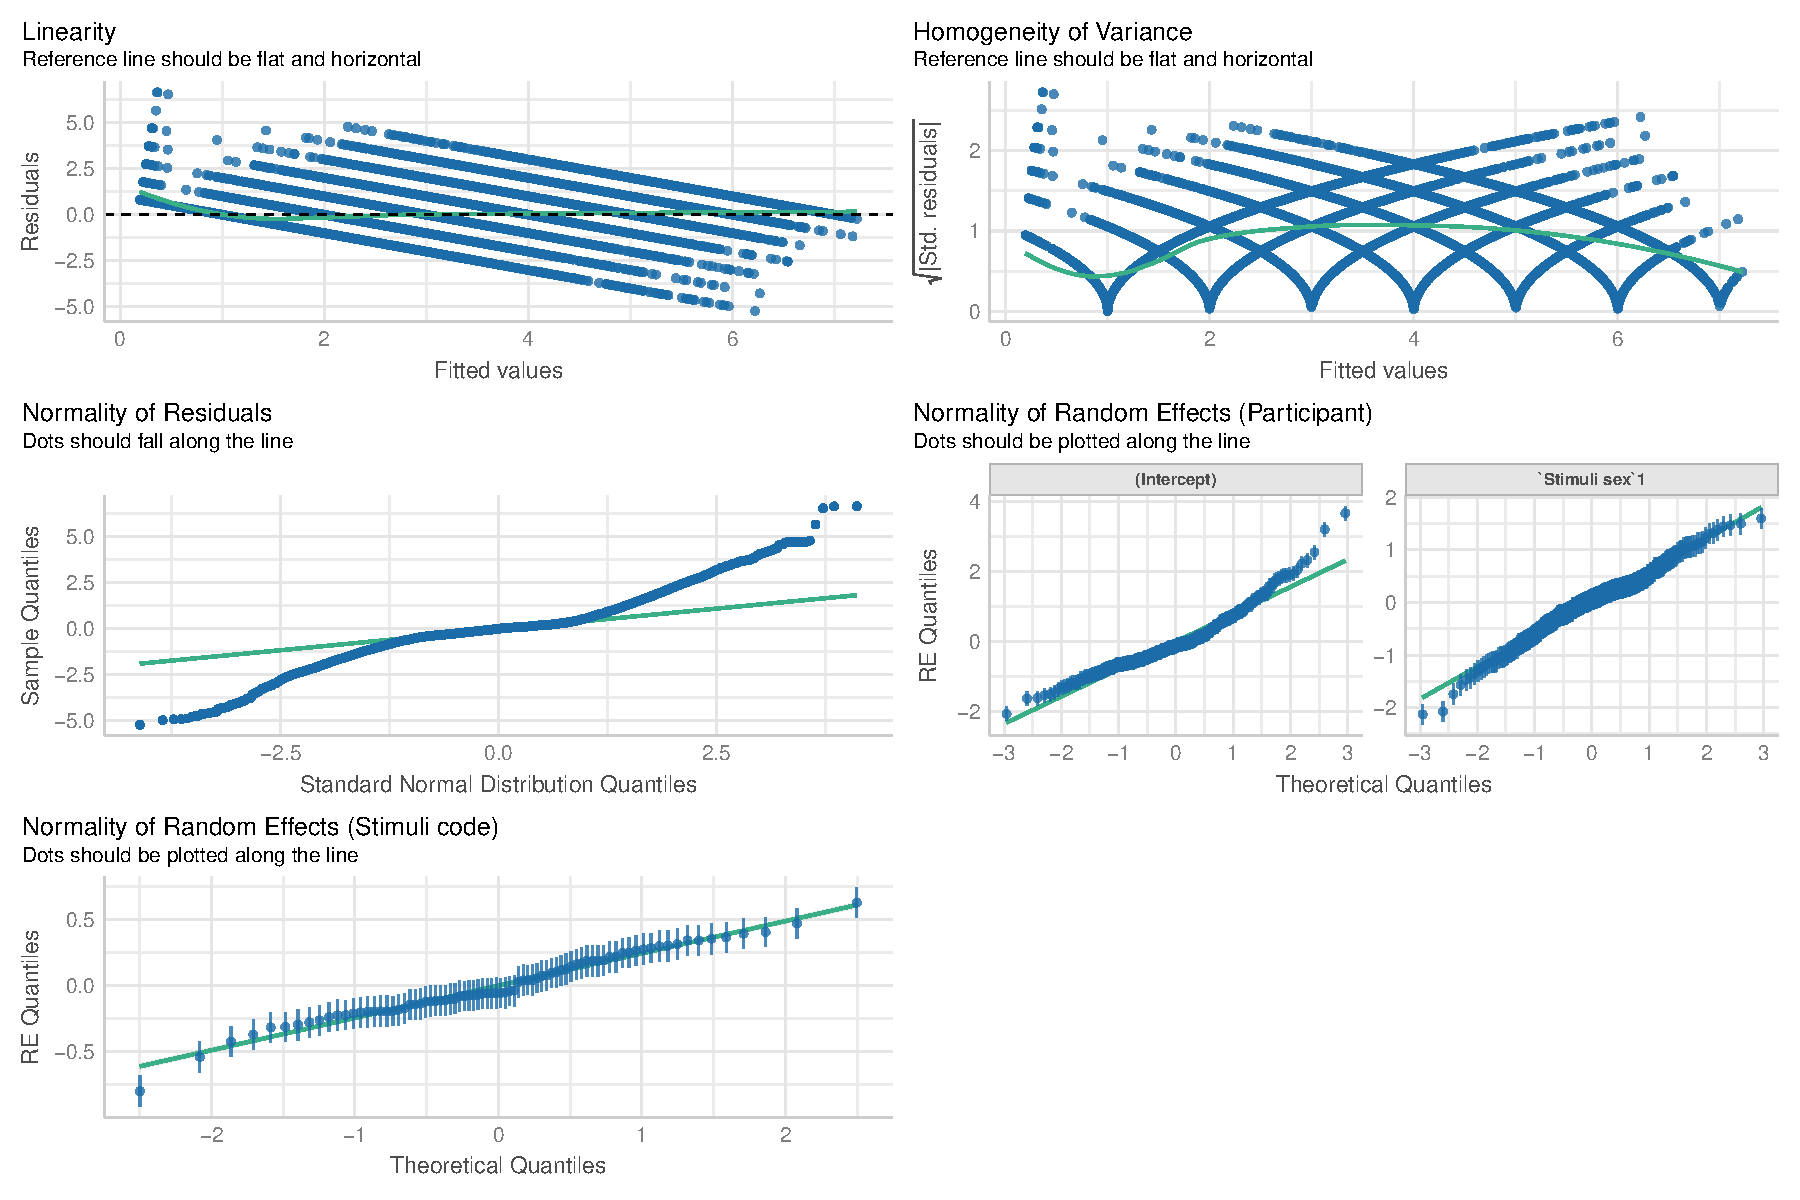
\includegraphics{Deseo_excitacion_sexual_files/figure-latex/assu-m2a-1.pdf}
\caption{\label{fig:assu-m2a}Model assumptions. Plots represent linearity, homogeneity of variance, and normality of both residuals and random effects (as QQ plots), respectively.}
\end{figure}

Table \ref{tab:coli-m2a}. Collinearity

Given the presence of interactions, that all predictors are categorical, and the absence of random slopes, \(VIF\) and \(GVIF\) values would be expected to be high.

\begin{Shaded}
\begin{Highlighting}[]
\FunctionTok{data.frame}\NormalTok{(}\FunctionTok{vif}\NormalTok{(m2a)) }\SpecialCharTok{|\textgreater{}} 
  \FunctionTok{rownames\_to\_column}\NormalTok{() }\SpecialCharTok{|\textgreater{}} 
  \FunctionTok{mutate\_at}\NormalTok{(}\StringTok{"rowname"}\NormalTok{, str\_replace\_all, }\StringTok{":"}\NormalTok{, }\StringTok{" × "}\NormalTok{) }\SpecialCharTok{|\textgreater{}}
  \FunctionTok{mutate\_at}\NormalTok{(}\StringTok{"rowname"}\NormalTok{, str\_replace\_all, }\StringTok{"\textasciigrave{}"}\NormalTok{, }\StringTok{""}\NormalTok{) }\SpecialCharTok{|\textgreater{}} 
  \FunctionTok{kable}\NormalTok{(}\AttributeTok{digits =} \DecValTok{2}\NormalTok{,}
        \AttributeTok{booktabs =} \ConstantTok{TRUE}\NormalTok{,}
        \AttributeTok{align =} \FunctionTok{c}\NormalTok{(}\StringTok{"l"}\NormalTok{, }\StringTok{"c"}\NormalTok{),}
        \AttributeTok{linesep =} \StringTok{""}\NormalTok{,}
        \AttributeTok{caption =} \StringTok{"Variance inflation factors for the model of hypothesis 2a"}\NormalTok{,}
        \AttributeTok{col.names =} \FunctionTok{c}\NormalTok{(}\StringTok{" "}\NormalTok{,}
                      \StringTok{"$VIF$"}\NormalTok{),}
        \AttributeTok{escape =} \ConstantTok{FALSE}\NormalTok{) }\SpecialCharTok{|\textgreater{}}
  \FunctionTok{kable\_styling}\NormalTok{(}\AttributeTok{latex\_options =} \StringTok{"HOLD\_position"}\NormalTok{)}
\end{Highlighting}
\end{Shaded}

\begin{table}[H]

\caption{\label{tab:coli-m2a}Variance inflation factors for the model of hypothesis 2a}
\centering
\begin{tabular}[t]{lc}
\toprule
  & $VIF$\\
\midrule
Relationship & 1.83\\
Gender & 1.82\\
Stimuli sex & 1.39\\
Solitary sexual desire (C) & 1.76\\
Dyadic sexual desire (Attractive person) (C) & 1.71\\
Dyadic sexual desire (Partner) (C) & 2.13\\
Relationship × Gender & 1.84\\
Relationship × Stimuli sex & 1.84\\
Gender × Stimuli sex & 1.83\\
Relationship × Solitary sexual desire (C) & 1.70\\
Gender × Solitary sexual desire (C) & 1.64\\
Stimuli sex × Solitary sexual desire (C) & 1.76\\
Relationship × Dyadic sexual desire (Attractive person) (C) & 1.65\\
Gender × Dyadic sexual desire (Attractive person) (C) & 1.54\\
Stimuli sex × Dyadic sexual desire (Attractive person) (C) & 1.71\\
Relationship × Dyadic sexual desire (Partner) (C) & 1.94\\
Gender × Dyadic sexual desire (Partner) (C) & 2.04\\
Stimuli sex × Dyadic sexual desire (Partner) (C) & 2.13\\
Relationship × Gender × Stimuli sex & 1.84\\
Relationship × Gender × Solitary sexual desire (C) & 1.72\\
Relationship × Stimuli sex × Solitary sexual desire (C) & 1.73\\
Gender × Stimuli sex × Solitary sexual desire (C) & 1.70\\
Relationship × Gender × Dyadic sexual desire (Attractive person) (C) & 1.69\\
Relationship × Stimuli sex × Dyadic sexual desire (Attractive person) (C) & 1.68\\
Gender × Stimuli sex × Dyadic sexual desire (Attractive person) (C) & 1.63\\
Relationship × Gender × Dyadic sexual desire (Partner) (C) & 2.12\\
Relationship × Stimuli sex × Dyadic sexual desire (Partner) (C) & 2.04\\
Gender × Stimuli sex × Dyadic sexual desire (Partner) (C) & 2.09\\
Relationship × Gender × Stimuli sex × Solitary sexual desire (C) & 1.74\\
Relationship × Gender × Stimuli sex × Dyadic sexual desire (Attractive person) (C) & 1.70\\
Relationship × Gender × Stimuli sex × Dyadic sexual desire (Partner) (C) & 2.12\\
\bottomrule
\end{tabular}
\end{table}

\hypertarget{bootstrap-confidence-intervals}{%
\subparagraph{Bootstrap confidence intervals}\label{bootstrap-confidence-intervals}}

\begin{Shaded}
\begin{Highlighting}[]
\NormalTok{m2aCI }\OtherTok{\textless{}{-}} \FunctionTok{confint}\NormalTok{(m2a, }
                 \AttributeTok{method =} \StringTok{"boot"}\NormalTok{, }\CommentTok{\#define bootstrap as the method for computing CIs}
                 \AttributeTok{nsim =} \DecValTok{4}\NormalTok{, }\CommentTok{\#number of simulations}
                 \AttributeTok{FUN =}\NormalTok{ fixef, }\CommentTok{\#to obtain only estimates for fixed effects}
                 \AttributeTok{parallel =} \StringTok{"multicore"}\NormalTok{, }\CommentTok{\#parallel computation}
                 \AttributeTok{ncpus =} \FunctionTok{detectCores}\NormalTok{()}\SpecialCharTok{{-}}\DecValTok{1}\NormalTok{, }\CommentTok{\#number of computational cores to run in parallel}
                 \AttributeTok{.progress =} \StringTok{"txt"}\NormalTok{, }\CommentTok{\#show progress bar}
                 \AttributeTok{seed =} \DecValTok{2023}\NormalTok{) }\CommentTok{\#to ensure reproducibility and allow cache to work}
\end{Highlighting}
\end{Shaded}

\begin{verbatim}
## ================================================================================
\end{verbatim}

\hypertarget{table-reftabtab-m2a.-regression-type-table-for-the-interaction-between-relationship-type-sexual-desire-dimension-and-gender}{%
\subparagraph{\texorpdfstring{Table \ref{tab:tab-m2a}. Regression-type table for the interaction between \texttt{Relationship\ type}, \texttt{Sexual\ desire\ dimension}, and \texttt{Gender}}{Table \ref{tab:tab-m2a}. Regression-type table for the interaction between Relationship type, Sexual desire dimension, and Gender}}\label{table-reftabtab-m2a.-regression-type-table-for-the-interaction-between-relationship-type-sexual-desire-dimension-and-gender}}

This tables summarizes the results of the model.

\begin{Shaded}
\begin{Highlighting}[]
\NormalTok{tab.m2a }\OtherTok{\textless{}{-}} \FunctionTok{summary.sig.boot}\NormalTok{(}\AttributeTok{mod =}\NormalTok{ m2a,}
                            \AttributeTok{modCI =}\NormalTok{ m2aCI,}
                            \AttributeTok{custom\_caption =} \StringTok{"Subjective sexual arousal in response to erotic }
\StringTok{                            stimuli, by relationship type, gender, stimuli sex, and the three }
\StringTok{                            dimensions of sexual desire dimension"}\NormalTok{)}
\NormalTok{tab.m2a}
\end{Highlighting}
\end{Shaded}

\begin{table}[H]

\caption{\label{tab:tab-m2a}Subjective sexual arousal in response to erotic 
                            stimuli, by relationship type, gender, stimuli sex, and the three 
                            dimensions of sexual desire dimension}
\centering
\resizebox{\linewidth}{!}{
\begin{threeparttable}
\begin{tabular}[t]{lccccccc}
\toprule
Effect & Estimate & Lower 95\% CI & Upper 95\% CI & Std. Error & $df$ & 
                        $t$ & $p$\\
\midrule
(Intercept) & 2.14 & 1.97 & 2.17 & 0.07 & 376.07 & 32.43 & \textbf{< 0.0001}\\
Relationship [Stable] & 0.05 & 0.04 & 0.06 & 0.06 & 304.00 & 0.77 & 0.44\\
Gender [Women] & -0.23 & -0.23 & -0.06 & 0.06 & 304.00 & -3.90 & \textbf{< 0.001}\\
Stimuli sex [Female] & 0.46 & 0.43 & 0.51 & 0.05 & 360.27 & 8.50 & \textbf{< 0.0001}\\
Solitary sexual desire (C) & 0.02 & 0.01 & 0.04 & 0.01 & 304.00 & 2.53 & \textbf{0.0119}\\
Dyadic sexual desire (Attractive person) (C) & 0.03 & 0.02 & 0.04 & 0.01 & 304.00 & 4.74 & \textbf{< 0.0001}\\
Dyadic sexual desire (Partner) (C) & 0.00 & -0.01 & 0.00 & 0.01 & 304.00 & 0.36 & 0.72\\
Relationship [Stable] × Gender [Women] & 0.01 & -0.09 & 0.07 & 0.06 & 304.00 & 0.16 & 0.88\\
Relationship [Stable] × Stimuli sex [Female] & 0.02 & -0.09 & 0.03 & 0.05 & 304.00 & 0.45 & 0.65\\
Gender [Women] × Stimuli sex [Female] & -0.81 & -0.90 & -0.68 & 0.05 & 304.00 & -17.66 & \textbf{< 0.0001}\\
Relationship [Stable] × Solitary sexual desire (C) & 0.00 & 0.00 & 0.00 & 0.01 & 304.00 & -0.44 & 0.66\\
Gender [Women] × Solitary sexual desire (C) & 0.01 & 0.00 & 0.01 & 0.01 & 304.00 & 1.22 & 0.22\\
Stimuli sex [Female] × Solitary sexual desire (C) & -0.01 & -0.01 & 0.00 & 0.01 & 304.00 & -1.05 & 0.3\\
Relationship [Stable] × Dyadic sexual desire (Attractive person) (C) & 0.01 & 0.00 & 0.01 & 0.01 & 304.00 & 1.13 & 0.26\\
Gender [Women] × Dyadic sexual desire (Attractive person) (C) & 0.00 & -0.01 & 0.00 & 0.01 & 304.00 & -0.29 & 0.77\\
Stimuli sex [Female] × Dyadic sexual desire (Attractive person) (C) & 0.02 & 0.00 & 0.02 & 0.01 & 304.00 & 2.86 & \textbf{0.0045}\\
Relationship [Stable] × Dyadic sexual desire (Partner) (C) & 0.00 & -0.01 & 0.01 & 0.01 & 304.00 & -0.51 & 0.61\\
Gender [Women] × Dyadic sexual desire (Partner) (C) & -0.01 & -0.01 & 0.00 & 0.01 & 304.00 & -1.60 & 0.11\\
Stimuli sex [Female] × Dyadic sexual desire (Partner) (C) & 0.01 & 0.01 & 0.01 & 0.01 & 304.00 & 1.75 & 0.08\\
Relationship [Stable] × Gender [Women] × Stimuli sex [Female] & 0.00 & -0.10 & 0.09 & 0.05 & 304.00 & 0.04 & 0.97\\
Relationship [Stable] × Gender [Women] × Solitary sexual desire (C) & 0.00 & 0.00 & 0.01 & 0.01 & 304.00 & 0.36 & 0.72\\
Relationship [Stable] × Stimuli sex [Female] × Solitary sexual desire (C) & 0.00 & 0.00 & 0.00 & 0.01 & 304.00 & -0.46 & 0.65\\
Gender [Women] × Stimuli sex [Female] × Solitary sexual desire (C) & 0.00 & -0.01 & 0.00 & 0.01 & 304.00 & -0.12 & 0.91\\
Relationship [Stable] × Gender [Women] × Dyadic sexual desire (Attractive person) (C) & -0.01 & -0.01 & 0.00 & 0.01 & 304.00 & -1.29 & 0.2\\
Relationship [Stable] × Stimuli sex [Female] × Dyadic sexual desire (Attractive person) (C) & 0.01 & 0.01 & 0.02 & 0.01 & 304.00 & 1.90 & 0.06\\
Gender [Women] × Stimuli sex [Female] × Dyadic sexual desire (Attractive person) (C) & -0.02 & -0.03 & -0.02 & 0.01 & 304.00 & -4.33 & \textbf{< 0.0001}\\
Relationship [Stable] × Gender [Women] × Dyadic sexual desire (Partner) (C) & 0.01 & 0.01 & 0.02 & 0.01 & 304.00 & 2.20 & \textbf{0.0285}\\
Relationship [Stable] × Stimuli sex [Female] × Dyadic sexual desire (Partner) (C) & -0.01 & -0.01 & -0.01 & 0.01 & 304.00 & -2.11 & \textbf{0.0357}\\
Gender [Women] × Stimuli sex [Female] × Dyadic sexual desire (Partner) (C) & -0.01 & -0.01 & 0.00 & 0.01 & 304.00 & -1.08 & 0.28\\
Relationship [Stable] × Gender [Women] × Stimuli sex [Female] × Solitary sexual desire (C) & 0.00 & 0.00 & 0.01 & 0.01 & 304.00 & 0.78 & 0.44\\
Relationship [Stable] × Gender [Women] × Stimuli sex [Female] × Dyadic sexual desire (Attractive person) (C) & 0.00 & -0.01 & 0.00 & 0.01 & 304.00 & -0.06 & 0.95\\
Relationship [Stable] × Gender [Women] × Stimuli sex [Female] × Dyadic sexual desire (Partner) (C) & 0.00 & -0.01 & 0.00 & 0.01 & 304.00 & -0.61 & 0.54\\
\bottomrule
\end{tabular}
\begin{tablenotes}[para]
\item \textit{Note: } 
\item $R^2_{conditional}$ = 0.749, $R^2_{marginal}$ = 0.385. Results are from linear mixed models for main 
                              effects and interactions between sexual desire (SD) dimensions,
                              sex, and Stimuli sex.
                              Confidence intervales were calculated as the 2.5 and 97.5 
                              percentiles from bootstrap (1000 simulations).
                              Continuous variables were centered and scaled
                              (represented as \textbf{(C)} in variable names).
                              Gender = participants gender (women, men); 
                              Stimuli sex = sex of stimuli (female, male); 
                              Solitary SD = Solitary Sexual Desire;
                              Attractive person DSD = Dyadic Sexual Desire toward an 
                              Attractive person;
                              Partner DSD = Dyadic Sexual Desire toward partner.
                              \textit{Sum-to-zero} contrasts were used to display
                              \textit{p}-values that represent main effects and interactions 
                              in an ANOVA-type manner (i.e. the intercept is the grand mean of 
                              all cells, and estimates are differences between each category
                              mean and the mean of all categories).
                              As reference categories 
                              \textit{Single} was used for relationship status,
                              \textit{Men} for gender,
                              and \textit{Male} for stimuli sex. 
                              Contrasted levels are in square brackets. 
                              Significant effects are in bold.
\end{tablenotes}
\end{threeparttable}}
\end{table}

\hypertarget{simple-slope-analysis-and-post-hoc-comparisons}{%
\subparagraph{\texorpdfstring{Simple slope analysis and \emph{post-hoc} comparisons}{Simple slope analysis and post-hoc comparisons}}\label{simple-slope-analysis-and-post-hoc-comparisons}}

We further explored significant interactions between gender and stimuli sex using estimated marginal means, as well as comparing subjective sexual arousal between stimuli sex for each participant gender.

Table \ref{tab:tab-m2a-emms-c}. Estimated marginal means and contrasts of subjective arousal between stimuli sex by participant gender

Table of estimated marginal means and contrasts between stimuli sex for each participant gender. All estimated marginal means and contrasts were calculated using the \texttt{emmeans} function from the \texttt{emmeans} package (\protect\hyperlink{ref-emmeanscit}{Lenth, 2022}).

\begin{Shaded}
\begin{Highlighting}[]
\NormalTok{emms.m2a\_c }\OtherTok{\textless{}{-}} \FunctionTok{emmeans}\NormalTok{(m2a, }\SpecialCharTok{\textasciitilde{}} \FunctionTok{factor}\NormalTok{(}\StringTok{\textasciigrave{}}\AttributeTok{Stimuli sex}\StringTok{\textasciigrave{}}\NormalTok{) }\SpecialCharTok{|}\NormalTok{ Gender,}
                    \AttributeTok{adjust =} \StringTok{"bonferroni"}\NormalTok{) }\CommentTok{\#asymptotic degrees of freedom}

\NormalTok{emms.m2a\_c.tab }\OtherTok{\textless{}{-}} \FunctionTok{tibble}\NormalTok{(}\FunctionTok{data.frame}\NormalTok{(emms.m2a\_c)) }\SpecialCharTok{|\textgreater{}}
  \FunctionTok{rename}\NormalTok{(}\StringTok{"Stimuli sex"} \OtherTok{=}\NormalTok{ Stimuli.sex) }\SpecialCharTok{|\textgreater{}} 
  \FunctionTok{mutate}\NormalTok{(}\StringTok{"Subjective sexual arousal (p)"} \OtherTok{=}\NormalTok{ emmean)}

\NormalTok{t.m2a\_c }\OtherTok{\textless{}{-}} \FunctionTok{contr.stars}\NormalTok{(emms.m2a\_c) }\SpecialCharTok{|\textgreater{}} 
  \FunctionTok{mutate}\NormalTok{(}\AttributeTok{p.value =} \FunctionTok{pval.lev}\NormalTok{(p.value))}

\NormalTok{t.m2a\_c.f }\OtherTok{\textless{}{-}}\NormalTok{ t.m2a\_c }\SpecialCharTok{|\textgreater{}} 
  \FunctionTok{insertRows}\NormalTok{(}\DecValTok{2}\NormalTok{, }\AttributeTok{new =} \ConstantTok{NA}\NormalTok{)}

\FunctionTok{merge}\NormalTok{(emms.m2a\_c.tab, t.m2a\_c.f, }\AttributeTok{by =} \DecValTok{0}\NormalTok{, }\AttributeTok{all =} \ConstantTok{TRUE}\NormalTok{) }\SpecialCharTok{|\textgreater{}}
  \FunctionTok{select}\NormalTok{(}\SpecialCharTok{{-}}\FunctionTok{c}\NormalTok{(}\DecValTok{1}\NormalTok{,}\DecValTok{3}\NormalTok{,}\DecValTok{6}\NormalTok{,}\DecValTok{9}\NormalTok{,}\DecValTok{12}\NormalTok{,}\DecValTok{15}\NormalTok{,}\DecValTok{18}\NormalTok{)) }\SpecialCharTok{|\textgreater{}} 
  \FunctionTok{unite}\NormalTok{(Contrast, group1, group2, }\AttributeTok{sep =} \StringTok{" {-} "}\NormalTok{) }\SpecialCharTok{|\textgreater{}}
  \FunctionTok{mutate\_at}\NormalTok{(}\StringTok{"Contrast"}\NormalTok{, str\_replace\_all, }\StringTok{"NA {-} NA"}\NormalTok{, }\StringTok{" "}\NormalTok{) }\SpecialCharTok{|\textgreater{}} 
  \FunctionTok{kable}\NormalTok{(}\AttributeTok{digits =} \DecValTok{2}\NormalTok{,}
          \AttributeTok{booktabs =} \ConstantTok{TRUE}\NormalTok{,}
          \AttributeTok{align =} \FunctionTok{c}\NormalTok{(}\StringTok{"l"}\NormalTok{, }\FunctionTok{rep}\NormalTok{(}\StringTok{"c"}\NormalTok{, }\DecValTok{5}\NormalTok{), }\StringTok{"l"}\NormalTok{, }\FunctionTok{rep}\NormalTok{(}\StringTok{"c"}\NormalTok{, }\DecValTok{5}\NormalTok{)),}
          \AttributeTok{linesep =} \StringTok{""}\NormalTok{,}
          \AttributeTok{caption =} \StringTok{"Estimated marginal means of subjective sexual arousal for gender by}
\StringTok{        stimuli sex, in response to erotic stimuli"}\NormalTok{,}
          \AttributeTok{col.names =} \FunctionTok{c}\NormalTok{(}\StringTok{"Stimuli sex"}\NormalTok{,}
                        \StringTok{"EMM"}\NormalTok{,}
                        \StringTok{"$SE$"}\NormalTok{,}
                        \StringTok{"$2.5}\SpecialCharTok{\textbackslash{}\textbackslash{}}\StringTok{\% CI$"}\NormalTok{,}
                        \StringTok{"$97.5}\SpecialCharTok{\textbackslash{}\textbackslash{}}\StringTok{\% CI$"}\NormalTok{,}
                        \StringTok{"Contrast"}\NormalTok{,}
                        \StringTok{"Difference"}\NormalTok{,}
                        \StringTok{"$SE$"}\NormalTok{,}
                        \StringTok{"$z$"}\NormalTok{,}
                        \StringTok{"$p$"}\NormalTok{),}
          \AttributeTok{escape =} \ConstantTok{FALSE}\NormalTok{) }\SpecialCharTok{|\textgreater{}}
  \FunctionTok{pack\_rows}\NormalTok{(}\AttributeTok{group\_label =} \StringTok{"Women"}\NormalTok{,}
            \AttributeTok{start\_row =} \DecValTok{1}\NormalTok{,}
            \AttributeTok{end\_row =} \DecValTok{2}\NormalTok{,}
            \AttributeTok{bold =} \ConstantTok{TRUE}\NormalTok{) }\SpecialCharTok{|\textgreater{}}
  \FunctionTok{pack\_rows}\NormalTok{(}\AttributeTok{group\_label =} \StringTok{"Men"}\NormalTok{,}
            \AttributeTok{start\_row =} \DecValTok{3}\NormalTok{,}
            \AttributeTok{end\_row =} \DecValTok{4}\NormalTok{,}
            \AttributeTok{hline\_before =} \ConstantTok{TRUE}\NormalTok{,}
            \AttributeTok{bold =} \ConstantTok{TRUE}\NormalTok{) }\SpecialCharTok{|\textgreater{}}
  \FunctionTok{add\_header\_above}\NormalTok{(}\FunctionTok{c}\NormalTok{(}\StringTok{" "} \OtherTok{=} \DecValTok{5}\NormalTok{, }\StringTok{"Contrasts"} \OtherTok{=} \DecValTok{5}\NormalTok{)) }\SpecialCharTok{|\textgreater{}} 
  \FunctionTok{kable\_styling}\NormalTok{(}\AttributeTok{latex\_options =} \FunctionTok{c}\NormalTok{(}\StringTok{"HOLD\_position"}\NormalTok{, }\StringTok{"scale\_down"}\NormalTok{)) }\SpecialCharTok{|\textgreater{}}
  \FunctionTok{footnote}\NormalTok{(}\AttributeTok{general =} \StringTok{"EMM = estimated marginal mean.}
\StringTok{           No degrees of freedom are reported, as an asymptotic method was used. }
\StringTok{           Because of this, }\SpecialCharTok{\textbackslash{}\textbackslash{}\textbackslash{}\textbackslash{}}\StringTok{textit\{z\} rather that }\SpecialCharTok{\textbackslash{}\textbackslash{}\textbackslash{}\textbackslash{}}\StringTok{textit\{t\} scores are reported.}
\StringTok{           Bonferroni adjustment was used."}\NormalTok{,}
           \AttributeTok{threeparttable =} \ConstantTok{TRUE}\NormalTok{,}
           \AttributeTok{footnote\_as\_chunk =} \ConstantTok{TRUE}\NormalTok{,}
           \AttributeTok{escape =} \ConstantTok{FALSE}\NormalTok{)}
\end{Highlighting}
\end{Shaded}

\begin{table}[H]

\caption{\label{tab:tab-m2a-emms-c}Estimated marginal means of subjective sexual arousal for gender by
        stimuli sex, in response to erotic stimuli}
\centering
\resizebox{\linewidth}{!}{
\begin{threeparttable}
\begin{tabular}[t]{lccccclccc}
\toprule
\multicolumn{5}{c}{ } & \multicolumn{5}{c}{Contrasts} \\
\cmidrule(l{3pt}r{3pt}){6-10}
Stimuli sex & EMM & $SE$ & $2.5\% CI$ & $97.5\% CI$ & Contrast & Difference & $SE$ & $z$ & $p$\\
\midrule
\addlinespace[0.3em]
\multicolumn{10}{l}{\textbf{Women}}\\
\hspace{1em}Female & 1.55 & 0.12 & 1.29 & 1.81 & Female - Male & -0.71 & 0.13 & -5.50 & \textbf{< 0.0001}\\
\hspace{1em}Male & 2.26 & 0.09 & 2.07 & 2.45 &  &  &  &  & \\
\addlinespace[0.3em]
\hline
\multicolumn{10}{l}{\textbf{Men}}\\
\hspace{1em}Female & 3.64 & 0.14 & 3.32 & 3.96 & Female - Male & 2.54 & 0.15 & 16.44 & \textbf{< 0.0001}\\
\hspace{1em}Male & 1.10 & 0.10 & 0.87 & 1.33 &  &  &  &  & \\
\bottomrule
\end{tabular}
\begin{tablenotes}[para]
\item \textit{Note: } 
\item EMM = estimated marginal mean.
           No degrees of freedom are reported, as an asymptotic method was used. 
           Because of this, \textit{z} rather that \textit{t} scores are reported.
           Bonferroni adjustment was used.
\end{tablenotes}
\end{threeparttable}}
\end{table}

Table \ref{tab:tab-m2a-slo-d}. Slope for Dyadic sexual desire (Attractive person) on Subjective sexual arousal by stimuli sex

Table of estimated slopes for Dyadic sexual desire (Attractive person) on Subjective sexual arousal for each stimuli sex from model 2a. Dyadic sexual desire (Attractive person) values were centered. Slopes were calculated using the \texttt{sim\_slopes} function from the \texttt{interactions} package (\protect\hyperlink{ref-interactionscit}{Long, 2019}).

\begin{Shaded}
\begin{Highlighting}[]
\NormalTok{slop.m2a\_d }\OtherTok{\textless{}{-}} \FunctionTok{sim\_slopes}\NormalTok{(m2a,}
                         \AttributeTok{pred =} \StringTok{"Dyadic sexual desire (Attractive person) (C)"}\NormalTok{, }
                         \AttributeTok{modx =} \StringTok{"Stimuli sex"}\NormalTok{)}

\NormalTok{slop.m2a\_d.tab }\OtherTok{\textless{}{-}} \FunctionTok{data.frame}\NormalTok{(slop.m2a\_d}\SpecialCharTok{$}\NormalTok{slopes) }\SpecialCharTok{|\textgreater{}}
  \FunctionTok{select}\NormalTok{(}\DecValTok{1}\NormalTok{,}\DecValTok{2}\NormalTok{,}\DecValTok{4}\NormalTok{,}\DecValTok{5}\SpecialCharTok{:}\DecValTok{7}\NormalTok{) }\SpecialCharTok{|\textgreater{}}
  \FunctionTok{mutate}\NormalTok{(}\FunctionTok{across}\NormalTok{(}\DecValTok{2}\SpecialCharTok{:}\DecValTok{6}\NormalTok{, as.numeric)) }\SpecialCharTok{|\textgreater{}}
  \FunctionTok{mutate}\NormalTok{(}\FunctionTok{across}\NormalTok{(}\DecValTok{2}\SpecialCharTok{:}\DecValTok{5}\NormalTok{, round, }\DecValTok{3}\NormalTok{)) }\SpecialCharTok{|\textgreater{}}
  \FunctionTok{mutate}\NormalTok{(}\AttributeTok{sig =} \FunctionTok{pval.stars}\NormalTok{(p)) }\SpecialCharTok{|\textgreater{}}
  \FunctionTok{rename}\NormalTok{(}\StringTok{"Stimuli sex"} \OtherTok{=} \StringTok{"Value.of.Stimuli.sex"}\NormalTok{) }\SpecialCharTok{|\textgreater{}}
  \FunctionTok{rename}\NormalTok{(}\AttributeTok{Coefficient =}\NormalTok{ Est.)}

\NormalTok{slop.m2a\_d.tab[,}\SpecialCharTok{{-}}\FunctionTok{c}\NormalTok{(}\DecValTok{7}\NormalTok{)] }\SpecialCharTok{|\textgreater{}} 
  \FunctionTok{mutate}\NormalTok{(}\AttributeTok{p =} \FunctionTok{pval.lev}\NormalTok{(p)) }\SpecialCharTok{|\textgreater{}} 
  \FunctionTok{kable}\NormalTok{(}\AttributeTok{booktabs =} \ConstantTok{TRUE}\NormalTok{,}
        \AttributeTok{align =} \FunctionTok{c}\NormalTok{(}\StringTok{"l"}\NormalTok{, }\FunctionTok{rep}\NormalTok{(}\StringTok{"c"}\NormalTok{, }\DecValTok{5}\NormalTok{)),}
        \AttributeTok{caption =} \StringTok{"Slope for Dyadic sexual desire (Attractive person) on }
\StringTok{        Subjective sexual arousal by stimuli sex"}\NormalTok{,}
        \AttributeTok{col.names =} \FunctionTok{c}\NormalTok{(}\StringTok{"Stimuli sex"}\NormalTok{,}
                      \StringTok{"$B$"}\NormalTok{,}
                      \StringTok{"$2.5}\SpecialCharTok{\textbackslash{}\textbackslash{}}\StringTok{\% CI$"}\NormalTok{,}
                      \StringTok{"$97.5}\SpecialCharTok{\textbackslash{}\textbackslash{}}\StringTok{\% CI$"}\NormalTok{,}
                      \StringTok{"$t$"}\NormalTok{,}
                      \StringTok{"$p$"}\NormalTok{),}
        \AttributeTok{escape =} \ConstantTok{FALSE}\NormalTok{) }\SpecialCharTok{|\textgreater{}} 
  \FunctionTok{kable\_styling}\NormalTok{(}\AttributeTok{latex\_options =} \FunctionTok{c}\NormalTok{(}\StringTok{"HOLD\_position"}\NormalTok{)) }\SpecialCharTok{|\textgreater{}}
  \FunctionTok{footnote}\NormalTok{(}\AttributeTok{general =} \StringTok{"$B$ and $CIs$ are for unstandardized coefficient.}
\StringTok{           No intercept is reported as continuous predictors were centered}
\StringTok{           and are dependent on this specific sample."}\NormalTok{,}
           \AttributeTok{threeparttable =} \ConstantTok{TRUE}\NormalTok{,}
           \AttributeTok{footnote\_as\_chunk =} \ConstantTok{TRUE}\NormalTok{,}
           \AttributeTok{escape =} \ConstantTok{FALSE}\NormalTok{)}
\end{Highlighting}
\end{Shaded}

\begin{table}[H]

\caption{\label{tab:tab-m2a-slo-d}Slope for Dyadic sexual desire (Attractive person) on 
        Subjective sexual arousal by stimuli sex}
\centering
\begin{threeparttable}
\begin{tabular}[t]{lccccc}
\toprule
Stimuli sex & $B$ & $2.5\% CI$ & $97.5\% CI$ & $t$ & $p$\\
\midrule
Male & 0.019 & 0.004 & 0.033 & 2.462 & \textbf{0.0144}\\
Female & 0.051 & 0.030 & 0.072 & 4.754 & \textbf{< 0.0001}\\
\bottomrule
\end{tabular}
\begin{tablenotes}[para]
\item \textit{Note: } 
\item $B$ and $CIs$ are for unstandardized coefficient.
           No intercept is reported as continuous predictors were centered
           and are dependent on this specific sample.
\end{tablenotes}
\end{threeparttable}
\end{table}

Table \ref{tab:tab-m2a-slo-e}. Slope for Dyadic sexual desire (Attractive person) on Subjective sexual arousal by stimuli sex and gender

Table of estimated slopes for Dyadic sexual desire (Attractive person) on Subjective sexual arousal for each stimuli sex and gender from model 2a. Dyadic sexual desire (Attractive person) values were centered. Slopes were calculated using the \texttt{sim\_slopes} function from the \texttt{interactions} package (\protect\hyperlink{ref-interactionscit}{Long, 2019}).

\begin{Shaded}
\begin{Highlighting}[]
\NormalTok{slop.m2a\_e }\OtherTok{\textless{}{-}} \FunctionTok{sim\_slopes}\NormalTok{(m2a, }
                         \AttributeTok{pred =} \StringTok{"Dyadic sexual desire (Attractive person) (C)"}\NormalTok{, }
                         \AttributeTok{mod2 =} \StringTok{"Gender"}\NormalTok{,}
                         \AttributeTok{modx =} \StringTok{"Stimuli sex"}\NormalTok{)}

\NormalTok{slop.m2a\_e.tab }\OtherTok{\textless{}{-}} \FunctionTok{rbind}\NormalTok{(}\FunctionTok{data.frame}\NormalTok{(slop.m2a\_e}\SpecialCharTok{$}\NormalTok{slopes[}\DecValTok{1}\NormalTok{]),}
                        \FunctionTok{data.frame}\NormalTok{(slop.m2a\_e}\SpecialCharTok{$}\NormalTok{slopes[}\DecValTok{2}\NormalTok{])) }\SpecialCharTok{|\textgreater{}}
  \FunctionTok{select}\NormalTok{(}\DecValTok{1}\NormalTok{,}\DecValTok{2}\NormalTok{,}\DecValTok{4}\NormalTok{,}\DecValTok{5}\SpecialCharTok{:}\DecValTok{7}\NormalTok{) }\SpecialCharTok{|\textgreater{}}
  \FunctionTok{mutate}\NormalTok{(}\FunctionTok{across}\NormalTok{(}\DecValTok{2}\SpecialCharTok{:}\DecValTok{6}\NormalTok{, as.numeric)) }\SpecialCharTok{|\textgreater{}}
  \FunctionTok{mutate}\NormalTok{(}\FunctionTok{across}\NormalTok{(}\DecValTok{2}\SpecialCharTok{:}\DecValTok{5}\NormalTok{, round, }\DecValTok{3}\NormalTok{)) }\SpecialCharTok{|\textgreater{}}
  \FunctionTok{mutate}\NormalTok{(}\AttributeTok{sig =} \FunctionTok{pval.stars}\NormalTok{(p)) }\SpecialCharTok{|\textgreater{}} 
  \FunctionTok{rename}\NormalTok{(}\StringTok{"Stimuli sex"} \OtherTok{=} \StringTok{"Value.of.Stimuli.sex"}\NormalTok{) }\SpecialCharTok{|\textgreater{}}
  \FunctionTok{rename}\NormalTok{(}\AttributeTok{Coefficient =}\NormalTok{ Est.) }\SpecialCharTok{|\textgreater{}} 
  \FunctionTok{mutate}\NormalTok{(}\AttributeTok{Gender =} \FunctionTok{rep}\NormalTok{(}\FunctionTok{c}\NormalTok{(}\StringTok{"Women"}\NormalTok{, }\StringTok{"Men"}\NormalTok{), }\AttributeTok{each =} \DecValTok{2}\NormalTok{)) }\SpecialCharTok{|\textgreater{}}
  \FunctionTok{select}\NormalTok{(}\DecValTok{8}\NormalTok{,}\DecValTok{1}\SpecialCharTok{:}\DecValTok{7}\NormalTok{)}

\NormalTok{slop.m2a\_e.tab[,}\SpecialCharTok{{-}}\FunctionTok{c}\NormalTok{(}\DecValTok{8}\NormalTok{)] }\SpecialCharTok{|\textgreater{}} 
  \FunctionTok{mutate}\NormalTok{(}\AttributeTok{p =} \FunctionTok{pval.lev}\NormalTok{(p)) }\SpecialCharTok{|\textgreater{}} 
  \FunctionTok{kable}\NormalTok{(}\AttributeTok{booktabs =} \ConstantTok{TRUE}\NormalTok{,}
        \AttributeTok{align =} \FunctionTok{c}\NormalTok{(}\StringTok{"l"}\NormalTok{, }\StringTok{"l"}\NormalTok{, }\FunctionTok{rep}\NormalTok{(}\StringTok{"c"}\NormalTok{, }\DecValTok{4}\NormalTok{)),}
        \AttributeTok{caption =} \StringTok{"Slope for Dyadic sexual desire (Attractive person) on }
\StringTok{        Subjective sexual arousal by stimuli sex and gender"}\NormalTok{,}
        \AttributeTok{col.names =} \FunctionTok{c}\NormalTok{(}\StringTok{"Gender"}\NormalTok{,}
                      \StringTok{"Stimuli sex"}\NormalTok{,}
                      \StringTok{"$B$"}\NormalTok{,}
                      \StringTok{"$2.5}\SpecialCharTok{\textbackslash{}\textbackslash{}}\StringTok{\% CI$"}\NormalTok{,}
                      \StringTok{"$97.5}\SpecialCharTok{\textbackslash{}\textbackslash{}}\StringTok{\% CI$"}\NormalTok{,}
                      \StringTok{"$t$"}\NormalTok{,}
                      \StringTok{"$p$"}\NormalTok{),}
        \AttributeTok{escape =} \ConstantTok{FALSE}\NormalTok{) }\SpecialCharTok{|\textgreater{}} 
  \FunctionTok{collapse\_rows}\NormalTok{(}\AttributeTok{columns =} \DecValTok{1}\NormalTok{, }\AttributeTok{valign =} \StringTok{"middle"}\NormalTok{) }\SpecialCharTok{|\textgreater{}} 
  \FunctionTok{kable\_styling}\NormalTok{(}\AttributeTok{latex\_options =} \FunctionTok{c}\NormalTok{(}\StringTok{"HOLD\_position"}\NormalTok{)) }\SpecialCharTok{|\textgreater{}}
  \FunctionTok{footnote}\NormalTok{(}\AttributeTok{general =} \StringTok{"$B$ and $CIs$ are for unstandardized coefficient.}
\StringTok{           No intercept is reported as continuous predictors were centered}
\StringTok{           and are dependent on this specific sample."}\NormalTok{,}
           \AttributeTok{threeparttable =} \ConstantTok{TRUE}\NormalTok{,}
           \AttributeTok{footnote\_as\_chunk =} \ConstantTok{TRUE}\NormalTok{,}
           \AttributeTok{escape =} \ConstantTok{FALSE}\NormalTok{)}
\end{Highlighting}
\end{Shaded}

\begin{table}[H]

\caption{\label{tab:tab-m2a-slo-e}Slope for Dyadic sexual desire (Attractive person) on 
        Subjective sexual arousal by stimuli sex and gender}
\centering
\begin{threeparttable}
\begin{tabular}[t]{llccccl}
\toprule
Gender & Stimuli sex & $B$ & $2.5\% CI$ & $97.5\% CI$ & $t$ & $p$\\
\midrule
 & Female & 0.024 & -0.002 & 0.051 & 1.802 & 0.07\\
\cmidrule{2-7}
\multirow{-2}{*}{\raggedright\arraybackslash Women} & Male & 0.041 & 0.022 & 0.060 & 4.316 & \textbf{< 0.0001}\\
\cmidrule{1-7}
 & Female & 0.077 & 0.045 & 0.110 & 4.658 & \textbf{< 0.0001}\\
\cmidrule{2-7}
\multirow{-2}{*}{\raggedright\arraybackslash Men} & Male & -0.004 & -0.027 & 0.019 & -0.328 & 0.74\\
\bottomrule
\end{tabular}
\begin{tablenotes}[para]
\item \textit{Note: } 
\item $B$ and $CIs$ are for unstandardized coefficient.
           No intercept is reported as continuous predictors were centered
           and are dependent on this specific sample.
\end{tablenotes}
\end{threeparttable}
\end{table}

Table \ref{tab:tab-m2a-slo-f}. Slope for Dyadic sexual desire (Partner) on Subjective sexual arousal by relationship type and gender

Table of estimated slopes for Dyadic sexual desire (Partner) on Subjective sexual arousal for each relationship type and gender from model 2a. Dyadic sexual desire (Partner) were centered Slopes were calculated using the \texttt{sim\_slopes} function from the \texttt{interactions} package (\protect\hyperlink{ref-interactionscit}{Long, 2019}).

\begin{Shaded}
\begin{Highlighting}[]
\NormalTok{slop.m2a\_f }\OtherTok{\textless{}{-}} \FunctionTok{sim\_slopes}\NormalTok{(m2a, }
                         \AttributeTok{pred =} \StringTok{"Dyadic sexual desire (Partner) (C)"}\NormalTok{, }
                         \AttributeTok{mod2 =} \StringTok{"Gender"}\NormalTok{,}
                         \AttributeTok{modx =} \StringTok{"Relationship"}\NormalTok{)}

\NormalTok{slop.m2a\_f.tab }\OtherTok{\textless{}{-}} \FunctionTok{rbind}\NormalTok{(}\FunctionTok{data.frame}\NormalTok{(slop.m2a\_f}\SpecialCharTok{$}\NormalTok{slopes[}\DecValTok{1}\NormalTok{]),}
                        \FunctionTok{data.frame}\NormalTok{(slop.m2a\_f}\SpecialCharTok{$}\NormalTok{slopes[}\DecValTok{2}\NormalTok{])) }\SpecialCharTok{|\textgreater{}}
  \FunctionTok{select}\NormalTok{(}\DecValTok{1}\NormalTok{,}\DecValTok{2}\NormalTok{,}\DecValTok{4}\NormalTok{,}\DecValTok{5}\SpecialCharTok{:}\DecValTok{7}\NormalTok{) }\SpecialCharTok{|\textgreater{}}
  \FunctionTok{mutate}\NormalTok{(}\FunctionTok{across}\NormalTok{(}\DecValTok{2}\SpecialCharTok{:}\DecValTok{6}\NormalTok{, as.numeric)) }\SpecialCharTok{|\textgreater{}}
  \FunctionTok{mutate}\NormalTok{(}\FunctionTok{across}\NormalTok{(}\DecValTok{2}\SpecialCharTok{:}\DecValTok{5}\NormalTok{, round, }\DecValTok{3}\NormalTok{)) }\SpecialCharTok{|\textgreater{}}
  \FunctionTok{mutate}\NormalTok{(}\AttributeTok{sig =} \FunctionTok{pval.stars}\NormalTok{(p)) }\SpecialCharTok{|\textgreater{}} 
  \FunctionTok{rename}\NormalTok{(}\StringTok{"Relationship"} \OtherTok{=} \StringTok{"Value.of.Relationship"}\NormalTok{) }\SpecialCharTok{|\textgreater{}}
  \FunctionTok{rename}\NormalTok{(}\AttributeTok{Coefficient =}\NormalTok{ Est.) }\SpecialCharTok{|\textgreater{}} 
  \FunctionTok{mutate}\NormalTok{(}\AttributeTok{Gender =} \FunctionTok{rep}\NormalTok{(}\FunctionTok{c}\NormalTok{(}\StringTok{"Women"}\NormalTok{, }\StringTok{"Men"}\NormalTok{), }\AttributeTok{each =} \DecValTok{2}\NormalTok{)) }\SpecialCharTok{|\textgreater{}}
  \FunctionTok{select}\NormalTok{(}\DecValTok{8}\NormalTok{,}\DecValTok{1}\SpecialCharTok{:}\DecValTok{7}\NormalTok{)}

\NormalTok{slop.m2a\_f.tab[,}\SpecialCharTok{{-}}\FunctionTok{c}\NormalTok{(}\DecValTok{8}\NormalTok{)] }\SpecialCharTok{|\textgreater{}} 
  \FunctionTok{mutate}\NormalTok{(}\AttributeTok{p =} \FunctionTok{pval.lev}\NormalTok{(p)) }\SpecialCharTok{|\textgreater{}} 
  \FunctionTok{kable}\NormalTok{(}\AttributeTok{booktabs =} \ConstantTok{TRUE}\NormalTok{,}
        \AttributeTok{align =} \FunctionTok{c}\NormalTok{(}\StringTok{"l"}\NormalTok{, }\StringTok{"l"}\NormalTok{, }\FunctionTok{rep}\NormalTok{(}\StringTok{"c"}\NormalTok{, }\DecValTok{5}\NormalTok{)),}
        \AttributeTok{caption =} \StringTok{"Slope for Dyadic sexual desire (Partner) on }
\StringTok{        Subjective sexual arousal by relationship type and gender"}\NormalTok{,}
        \AttributeTok{col.names =} \FunctionTok{c}\NormalTok{(}\StringTok{"Gender"}\NormalTok{,}
                      \StringTok{"Relationship"}\NormalTok{,}
                      \StringTok{"$B$"}\NormalTok{,}
                      \StringTok{"$2.5}\SpecialCharTok{\textbackslash{}\textbackslash{}}\StringTok{\% CI$"}\NormalTok{,}
                      \StringTok{"$97.5}\SpecialCharTok{\textbackslash{}\textbackslash{}}\StringTok{\% CI$"}\NormalTok{,}
                      \StringTok{"$t$"}\NormalTok{,}
                      \StringTok{"$p$"}\NormalTok{),}
        \AttributeTok{escape =} \ConstantTok{FALSE}\NormalTok{) }\SpecialCharTok{|\textgreater{}} 
  \FunctionTok{collapse\_rows}\NormalTok{(}\AttributeTok{columns =} \DecValTok{1}\NormalTok{, }\AttributeTok{valign =} \StringTok{"middle"}\NormalTok{) }\SpecialCharTok{|\textgreater{}} 
  \FunctionTok{kable\_styling}\NormalTok{(}\AttributeTok{latex\_options =} \FunctionTok{c}\NormalTok{(}\StringTok{"HOLD\_position"}\NormalTok{)) }\SpecialCharTok{|\textgreater{}}
  \FunctionTok{footnote}\NormalTok{(}\AttributeTok{general =} \StringTok{"$B$ and $CIs$ are for unstandardized coefficient.}
\StringTok{           No intercept is reported as continuous predictors were centered}
\StringTok{           and are dependent on this specific sample."}\NormalTok{,}
           \AttributeTok{threeparttable =} \ConstantTok{TRUE}\NormalTok{,}
           \AttributeTok{footnote\_as\_chunk =} \ConstantTok{TRUE}\NormalTok{,}
           \AttributeTok{escape =} \ConstantTok{FALSE}\NormalTok{)}
\end{Highlighting}
\end{Shaded}

\begin{table}[H]

\caption{\label{tab:tab-m2a-slo-f}Slope for Dyadic sexual desire (Partner) on 
        Subjective sexual arousal by relationship type and gender}
\centering
\begin{threeparttable}
\begin{tabular}[t]{llccccc}
\toprule
Gender & Relationship & $B$ & $2.5\% CI$ & $97.5\% CI$ & $t$ & $p$\\
\midrule
 & Stable & 0.003 & -0.017 & 0.023 & 0.309 & 0.76\\
\cmidrule{2-7}
\multirow{-2}{*}{\raggedright\arraybackslash Women} & Single & -0.020 & -0.042 & 0.002 & -1.803 & 0.07\\
\cmidrule{1-7}
 & Stable & -0.005 & -0.042 & 0.032 & -0.267 & 0.79\\
\cmidrule{2-7}
\multirow{-2}{*}{\raggedright\arraybackslash Men} & Single & 0.032 & 0.007 & 0.057 & 2.529 & \textbf{0.012}\\
\bottomrule
\end{tabular}
\begin{tablenotes}[para]
\item \textit{Note: } 
\item $B$ and $CIs$ are for unstandardized coefficient.
           No intercept is reported as continuous predictors were centered
           and are dependent on this specific sample.
\end{tablenotes}
\end{threeparttable}
\end{table}

Table \ref{tab:tab-m2a-slo-g}. Slope for Dyadic sexual desire (Partner) on Subjective sexual arousal by relationship type and stimuli sex

Table of estimated slopes for Dyadic sexual desire (Partner) on Subjective sexual arousal for each relationship type and stimuli sex from model 2a. Dyadic sexual desire (Partner) were centered Slopes were calculated using the \texttt{sim\_slopes} function from the \texttt{interactions} package (\protect\hyperlink{ref-interactionscit}{Long, 2019}).

\begin{Shaded}
\begin{Highlighting}[]
\NormalTok{slop.m2a\_g }\OtherTok{\textless{}{-}} \FunctionTok{sim\_slopes}\NormalTok{(m2a, }
                         \AttributeTok{pred =} \StringTok{"Dyadic sexual desire (Partner) (C)"}\NormalTok{, }
                         \AttributeTok{mod2 =} \StringTok{"Stimuli sex"}\NormalTok{,}
                         \AttributeTok{modx =} \StringTok{"Relationship"}\NormalTok{)}

\NormalTok{slop.m2a\_g.tab }\OtherTok{\textless{}{-}} \FunctionTok{rbind}\NormalTok{(}\FunctionTok{data.frame}\NormalTok{(slop.m2a\_g}\SpecialCharTok{$}\NormalTok{slopes[}\DecValTok{1}\NormalTok{]),}
                        \FunctionTok{data.frame}\NormalTok{(slop.m2a\_g}\SpecialCharTok{$}\NormalTok{slopes[}\DecValTok{2}\NormalTok{])) }\SpecialCharTok{|\textgreater{}}
  \FunctionTok{select}\NormalTok{(}\DecValTok{1}\NormalTok{,}\DecValTok{2}\NormalTok{,}\DecValTok{4}\NormalTok{,}\DecValTok{5}\SpecialCharTok{:}\DecValTok{7}\NormalTok{) }\SpecialCharTok{|\textgreater{}}
  \FunctionTok{mutate}\NormalTok{(}\FunctionTok{across}\NormalTok{(}\DecValTok{2}\SpecialCharTok{:}\DecValTok{6}\NormalTok{, as.numeric)) }\SpecialCharTok{|\textgreater{}}
  \FunctionTok{mutate}\NormalTok{(}\FunctionTok{across}\NormalTok{(}\DecValTok{2}\SpecialCharTok{:}\DecValTok{5}\NormalTok{, round, }\DecValTok{3}\NormalTok{)) }\SpecialCharTok{|\textgreater{}}
  \FunctionTok{mutate}\NormalTok{(}\AttributeTok{sig =} \FunctionTok{pval.stars}\NormalTok{(p)) }\SpecialCharTok{|\textgreater{}} 
  \FunctionTok{rename}\NormalTok{(}\StringTok{"Relationship"} \OtherTok{=} \StringTok{"Value.of.Relationship"}\NormalTok{) }\SpecialCharTok{|\textgreater{}}
  \FunctionTok{rename}\NormalTok{(}\AttributeTok{Coefficient =}\NormalTok{ Est.) }\SpecialCharTok{|\textgreater{}} 
  \FunctionTok{mutate}\NormalTok{(}\StringTok{"Stimuli sex"} \OtherTok{=} \FunctionTok{rep}\NormalTok{(}\FunctionTok{c}\NormalTok{(}\StringTok{"Female"}\NormalTok{, }\StringTok{"Male"}\NormalTok{), }\AttributeTok{each =} \DecValTok{2}\NormalTok{)) }\SpecialCharTok{|\textgreater{}}
  \FunctionTok{select}\NormalTok{(}\DecValTok{8}\NormalTok{,}\DecValTok{1}\SpecialCharTok{:}\DecValTok{7}\NormalTok{)}

\NormalTok{slop.m2a\_g.tab[,}\SpecialCharTok{{-}}\FunctionTok{c}\NormalTok{(}\DecValTok{8}\NormalTok{)] }\SpecialCharTok{|\textgreater{}} 
  \FunctionTok{mutate}\NormalTok{(}\AttributeTok{p =} \FunctionTok{pval.lev}\NormalTok{(p)) }\SpecialCharTok{|\textgreater{}} 
  \FunctionTok{kable}\NormalTok{(}\AttributeTok{booktabs =} \ConstantTok{TRUE}\NormalTok{,}
        \AttributeTok{align =} \FunctionTok{c}\NormalTok{(}\StringTok{"l"}\NormalTok{, }\StringTok{"l"}\NormalTok{, }\FunctionTok{rep}\NormalTok{(}\StringTok{"c"}\NormalTok{, }\DecValTok{4}\NormalTok{)),}
        \AttributeTok{caption =} \StringTok{"Slope for Dyadic sexual desire (Partner) on }
\StringTok{        Subjective sexual arousal by relationship type and stimuli sex"}\NormalTok{,}
        \AttributeTok{col.names =} \FunctionTok{c}\NormalTok{(}\StringTok{"Stimuli sex"}\NormalTok{,}
                      \StringTok{"Relationship"}\NormalTok{,}
                      \StringTok{"$B$"}\NormalTok{,}
                      \StringTok{"$2.5}\SpecialCharTok{\textbackslash{}\textbackslash{}}\StringTok{\% CI$"}\NormalTok{,}
                      \StringTok{"$97.5}\SpecialCharTok{\textbackslash{}\textbackslash{}}\StringTok{\% CI$"}\NormalTok{,}
                      \StringTok{"$t$"}\NormalTok{,}
                      \StringTok{"$p$"}\NormalTok{),}
        \AttributeTok{escape =} \ConstantTok{FALSE}\NormalTok{) }\SpecialCharTok{|\textgreater{}} 
  \FunctionTok{collapse\_rows}\NormalTok{(}\AttributeTok{columns =} \DecValTok{1}\NormalTok{, }\AttributeTok{valign =} \StringTok{"middle"}\NormalTok{) }\SpecialCharTok{|\textgreater{}} 
  \FunctionTok{kable\_styling}\NormalTok{(}\AttributeTok{latex\_options =} \FunctionTok{c}\NormalTok{(}\StringTok{"HOLD\_position"}\NormalTok{)) }\SpecialCharTok{|\textgreater{}}
  \FunctionTok{footnote}\NormalTok{(}\AttributeTok{general =} \StringTok{"$B$ and $CIs$ are for unstandardized coefficient.}
\StringTok{           No intercept is reported as continuous predictors were centered}
\StringTok{           and are dependent on this specific sample."}\NormalTok{,}
           \AttributeTok{threeparttable =} \ConstantTok{TRUE}\NormalTok{,}
           \AttributeTok{footnote\_as\_chunk =} \ConstantTok{TRUE}\NormalTok{,}
           \AttributeTok{escape =} \ConstantTok{FALSE}\NormalTok{)}
\end{Highlighting}
\end{Shaded}

\begin{table}[H]

\caption{\label{tab:tab-m2a-slo-g}Slope for Dyadic sexual desire (Partner) on 
        Subjective sexual arousal by relationship type and stimuli sex}
\centering
\begin{threeparttable}
\begin{tabular}[t]{llccccl}
\toprule
Stimuli sex & Relationship & $B$ & $2.5\% CI$ & $97.5\% CI$ & $t$ & $p$\\
\midrule
 & Stable & -0.003 & -0.034 & 0.028 & -0.182 & 0.86\\
\cmidrule{2-7}
\multirow{-2}{*}{\raggedright\arraybackslash Female} & Single & 0.026 & 0.002 & 0.050 & 2.144 & \textbf{0.0329}\\
\cmidrule{1-7}
 & Stable & 0.001 & -0.021 & 0.023 & 0.081 & 0.94\\
\cmidrule{2-7}
\multirow{-2}{*}{\raggedright\arraybackslash Male} & Single & -0.014 & -0.031 & 0.003 & -1.665 & 0.1\\
\bottomrule
\end{tabular}
\begin{tablenotes}[para]
\item \textit{Note: } 
\item $B$ and $CIs$ are for unstandardized coefficient.
           No intercept is reported as continuous predictors were centered
           and are dependent on this specific sample.
\end{tablenotes}
\end{threeparttable}
\end{table}

\hypertarget{figure-reffigfig-h2a.-subjective-sexual-arousal-to-erotic-stimuli-main-effects-and-interactions}{%
\paragraph{Figure \ref{fig:fig-h2a}. Subjective sexual arousal to erotic stimuli: Main effects and interactions}\label{figure-reffigfig-h2a.-subjective-sexual-arousal-to-erotic-stimuli-main-effects-and-interactions}}

This figure summarizes the results of hypothesis 2a.

\begin{Shaded}
\begin{Highlighting}[]
\DocumentationTok{\#\# Create data frame and add predicted values for plots}
\NormalTok{m2a.dat }\OtherTok{\textless{}{-}}\NormalTok{ m2a}\SpecialCharTok{@}\NormalTok{frame }\SpecialCharTok{|\textgreater{}} 
  \FunctionTok{mutate}\NormalTok{(}\StringTok{\textasciigrave{}}\AttributeTok{Subjective sexual arousal (p)}\StringTok{\textasciigrave{}} \OtherTok{=} \FunctionTok{predict}\NormalTok{(m2a))}

\DocumentationTok{\#\# Extract slope data from model summary for main effects of continuous predictors}
\NormalTok{slop.m2a\_ab.tab }\OtherTok{\textless{}{-}} \FunctionTok{left\_join}\NormalTok{(}\FunctionTok{data.frame}\NormalTok{(}\FunctionTok{summary}\NormalTok{(m2a)}\SpecialCharTok{$}\NormalTok{coefficients) }\SpecialCharTok{|\textgreater{}}
                               \FunctionTok{rownames\_to\_column}\NormalTok{(),}
                             \FunctionTok{data.frame}\NormalTok{(m2aCI) }\SpecialCharTok{|\textgreater{}}
                               \FunctionTok{rownames\_to\_column}\NormalTok{(),}
                             \AttributeTok{by =} \StringTok{"rowname"}\NormalTok{)[}\DecValTok{5}\SpecialCharTok{:}\DecValTok{6}\NormalTok{,] }\SpecialCharTok{|\textgreater{}}
  \FunctionTok{select}\NormalTok{(}\DecValTok{1}\SpecialCharTok{:}\DecValTok{2}\NormalTok{,}\DecValTok{7}\SpecialCharTok{:}\DecValTok{8}\NormalTok{,}\DecValTok{5}\SpecialCharTok{:}\DecValTok{6}\NormalTok{) }\SpecialCharTok{|\textgreater{}}
  \FunctionTok{mutate}\NormalTok{(}\FunctionTok{across}\NormalTok{(}\DecValTok{2}\SpecialCharTok{:}\DecValTok{5}\NormalTok{, round, }\DecValTok{3}\NormalTok{)) }\SpecialCharTok{|\textgreater{}}
  \FunctionTok{mutate}\NormalTok{(}\AttributeTok{Pr...t.. =} \FunctionTok{pval.lev2}\NormalTok{(Pr...t..))}

\CommentTok{\# Figure main effect of Solitary sexual desire on Subjective sexual arousal}
\NormalTok{p2a.a }\OtherTok{\textless{}{-}} \FunctionTok{ggplot}\NormalTok{(m2a.dat, }\FunctionTok{aes}\NormalTok{(}\AttributeTok{x =} \StringTok{\textasciigrave{}}\AttributeTok{Solitary sexual desire (C)}\StringTok{\textasciigrave{}}\NormalTok{, }
                             \AttributeTok{y =} \StringTok{\textasciigrave{}}\AttributeTok{Subjective sexual arousal (p)}\StringTok{\textasciigrave{}}\NormalTok{)) }\SpecialCharTok{+}
  \FunctionTok{geom\_jitter}\NormalTok{(}\AttributeTok{alpha =}  \FloatTok{0.01}\NormalTok{) }\SpecialCharTok{+}
  \FunctionTok{geom\_smooth}\NormalTok{(}\AttributeTok{method =} \StringTok{"lm"}\NormalTok{) }\SpecialCharTok{+}
  \FunctionTok{labs}\NormalTok{(}\AttributeTok{y =} \StringTok{"Subjective sexual}\SpecialCharTok{\textbackslash{}n}\StringTok{arousal (predicted)"}\NormalTok{) }\SpecialCharTok{+}
  \FunctionTok{geom\_text}\NormalTok{(}\AttributeTok{data =}\NormalTok{ slop.m2a\_ab.tab[}\DecValTok{1}\NormalTok{,],}
            \AttributeTok{mapping =} \FunctionTok{aes}\NormalTok{(}\AttributeTok{x =} \SpecialCharTok{{-}}\ConstantTok{Inf}\NormalTok{, }\AttributeTok{y =}\ConstantTok{Inf}\NormalTok{,}
                          \AttributeTok{vjust =} \DecValTok{2}\NormalTok{, }\AttributeTok{hjust =} \SpecialCharTok{{-}}\FloatTok{0.03}\NormalTok{),}
            \AttributeTok{label =} \FunctionTok{paste}\NormalTok{(}\StringTok{"B = "}\NormalTok{, slop.m2a\_ab.tab[}\DecValTok{1}\NormalTok{,]}\SpecialCharTok{$}\NormalTok{Estimate,}
                          \StringTok{", IC 95\%["}\NormalTok{,}
                          \FunctionTok{paste}\NormalTok{(slop.m2a\_ab.tab[}\DecValTok{1}\NormalTok{,]}\SpecialCharTok{$}\NormalTok{X2.}\DecValTok{5}\NormalTok{..,}
\NormalTok{                                slop.m2a\_ab.tab[}\DecValTok{1}\NormalTok{,]}\SpecialCharTok{$}\NormalTok{X97.}\DecValTok{5}\NormalTok{..,}
                                \AttributeTok{sep =} \StringTok{", "}\NormalTok{),}
                          \StringTok{"], p"}\NormalTok{, slop.m2a\_ab.tab[}\DecValTok{1}\NormalTok{,]}\SpecialCharTok{$}\NormalTok{Pr...t.., }\StringTok{"*"}\NormalTok{),}
            \AttributeTok{size =} \DecValTok{3}\NormalTok{) }\SpecialCharTok{+}
  \FunctionTok{theme\_tq}\NormalTok{()}

\CommentTok{\# Figure main effect of Dyadic sexual desire (Attractive person) on Subjective sexual arousal}
\NormalTok{p2a.b }\OtherTok{\textless{}{-}} \FunctionTok{ggplot}\NormalTok{(m2a.dat, }\FunctionTok{aes}\NormalTok{(}\AttributeTok{x =} \StringTok{\textasciigrave{}}\AttributeTok{Dyadic sexual desire (Attractive person) (C)}\StringTok{\textasciigrave{}}\NormalTok{, }
                             \AttributeTok{y =} \StringTok{\textasciigrave{}}\AttributeTok{Subjective sexual arousal (p)}\StringTok{\textasciigrave{}}\NormalTok{)) }\SpecialCharTok{+}
  \FunctionTok{geom\_jitter}\NormalTok{(}\AttributeTok{alpha =}  \FloatTok{0.01}\NormalTok{) }\SpecialCharTok{+}
  \FunctionTok{geom\_smooth}\NormalTok{(}\AttributeTok{method =} \StringTok{"lm"}\NormalTok{) }\SpecialCharTok{+}
  \FunctionTok{labs}\NormalTok{(}\AttributeTok{y =} \StringTok{" }\SpecialCharTok{\textbackslash{}n}\StringTok{ "}\NormalTok{)  }\SpecialCharTok{+}
  \FunctionTok{geom\_text}\NormalTok{(}\AttributeTok{data =}\NormalTok{ slop.m2a\_ab.tab[}\DecValTok{2}\NormalTok{,],}
            \AttributeTok{mapping =} \FunctionTok{aes}\NormalTok{(}\AttributeTok{x =} \SpecialCharTok{{-}}\ConstantTok{Inf}\NormalTok{, }\AttributeTok{y =} \ConstantTok{Inf}\NormalTok{,}
            \AttributeTok{vjust =} \DecValTok{2}\NormalTok{, }\AttributeTok{hjust =} \SpecialCharTok{{-}}\FloatTok{0.03}\NormalTok{),}
            \AttributeTok{label =} \FunctionTok{paste}\NormalTok{(}\StringTok{"B = "}\NormalTok{, slop.m2a\_ab.tab[}\DecValTok{2}\NormalTok{,]}\SpecialCharTok{$}\NormalTok{Estimate, }
                          \StringTok{", IC 95\%["}\NormalTok{, }\FunctionTok{paste}\NormalTok{(slop.m2a\_ab.tab[}\DecValTok{2}\NormalTok{,]}\SpecialCharTok{$}\NormalTok{X2.}\DecValTok{5}\NormalTok{..,}
\NormalTok{                                             slop.m2a\_ab.tab[}\DecValTok{2}\NormalTok{,]}\SpecialCharTok{$}\NormalTok{X97.}\DecValTok{5}\NormalTok{.., }
                                             \AttributeTok{sep =} \StringTok{", "}\NormalTok{), }
                          \StringTok{"], p"}\NormalTok{, slop.m2a\_ab.tab[}\DecValTok{2}\NormalTok{,]}\SpecialCharTok{$}\NormalTok{Pr...t.., }\StringTok{"****"}\NormalTok{),}
            \AttributeTok{size =} \DecValTok{3}\NormalTok{) }\SpecialCharTok{+}
  \FunctionTok{theme\_tq}\NormalTok{()}

\CommentTok{\# Figure interaction between Stimuli sex and gender}
\NormalTok{p2a.c }\OtherTok{\textless{}{-}} \FunctionTok{ggplot}\NormalTok{(m2a.dat, }\FunctionTok{aes}\NormalTok{(}\AttributeTok{x =} \StringTok{\textasciigrave{}}\AttributeTok{Stimuli sex}\StringTok{\textasciigrave{}}\NormalTok{, }
                             \AttributeTok{y =} \StringTok{\textasciigrave{}}\AttributeTok{Subjective sexual arousal (p)}\StringTok{\textasciigrave{}}\NormalTok{, }
                             \AttributeTok{color =} \StringTok{\textasciigrave{}}\AttributeTok{Stimuli sex}\StringTok{\textasciigrave{}}\NormalTok{)) }\SpecialCharTok{+}
  \FunctionTok{geom\_violin}\NormalTok{() }\SpecialCharTok{+}
  \FunctionTok{geom\_jitter}\NormalTok{(}\AttributeTok{alpha =} \FloatTok{0.01}\NormalTok{, }\AttributeTok{width =} \FloatTok{0.1}\NormalTok{) }\SpecialCharTok{+}
  \FunctionTok{scale\_color\_manual}\NormalTok{(}\AttributeTok{values =}\NormalTok{ color.StimuliSex) }\SpecialCharTok{+}
  \FunctionTok{scale\_fill\_manual}\NormalTok{(}\AttributeTok{values =}\NormalTok{ color.StimuliSex) }\SpecialCharTok{+}
  \FunctionTok{facet\_wrap}\NormalTok{(}\SpecialCharTok{\textasciitilde{}}\NormalTok{Gender) }\SpecialCharTok{+}
  \FunctionTok{geom\_errorbar}\NormalTok{(}\AttributeTok{data =}\NormalTok{ emms.m2a\_c.tab, }
                \AttributeTok{mapping =} \FunctionTok{aes}\NormalTok{(}\AttributeTok{ymin =}\NormalTok{ asymp.LCL, }\AttributeTok{ymax =}\NormalTok{ asymp.UCL), }
                \AttributeTok{colour =} \StringTok{"black"}\NormalTok{, }\AttributeTok{width =} \FloatTok{0.1}\NormalTok{) }\SpecialCharTok{+}
  \FunctionTok{geom\_point}\NormalTok{(}\AttributeTok{data =}\NormalTok{ emms.m2a\_c.tab, }
             \AttributeTok{shape =} \DecValTok{21}\NormalTok{, }\AttributeTok{size =} \DecValTok{3}\NormalTok{,}
             \AttributeTok{color =} \StringTok{"black"}\NormalTok{, }\AttributeTok{fill =} \StringTok{"white"}\NormalTok{) }\SpecialCharTok{+}
  \FunctionTok{stat\_pvalue\_manual}\NormalTok{(t.m2a\_c, }
                     \AttributeTok{label =} \StringTok{"p.signif"}\NormalTok{, }
                     \AttributeTok{y.position =} \FunctionTok{c}\NormalTok{(}\FloatTok{7.4}\NormalTok{,}\FloatTok{7.8}\NormalTok{), }
                     \AttributeTok{tip.length =} \DecValTok{0}\NormalTok{) }\SpecialCharTok{+}
  \FunctionTok{labs}\NormalTok{(}\AttributeTok{y =} \StringTok{"Subjective sexual}\SpecialCharTok{\textbackslash{}n}\StringTok{arousal (predicted)"}\NormalTok{) }\SpecialCharTok{+}
  \FunctionTok{ylim}\NormalTok{(}\FunctionTok{c}\NormalTok{(}\DecValTok{0}\NormalTok{, }\FloatTok{8.5}\NormalTok{)) }\SpecialCharTok{+}
  \FunctionTok{theme\_tq}\NormalTok{() }\SpecialCharTok{+}
  \FunctionTok{theme}\NormalTok{(}\AttributeTok{legend.position =} \StringTok{"none"}\NormalTok{)}

\CommentTok{\# Figure interaction between Stimuli sex and Dyadic sexual desire (Attractive person)}
\DocumentationTok{\#\# Extract data for by stimuli sex}
\NormalTok{slop.m2a\_d.tab\_f }\OtherTok{\textless{}{-}} \FunctionTok{filter}\NormalTok{(slop.m2a\_d.tab, }\StringTok{\textasciigrave{}}\AttributeTok{Stimuli sex}\StringTok{\textasciigrave{}} \SpecialCharTok{==} \StringTok{"Female"}\NormalTok{) }\SpecialCharTok{|\textgreater{}}
  \FunctionTok{mutate}\NormalTok{(}\AttributeTok{p =} \FunctionTok{pval.lev2}\NormalTok{(p))}
\NormalTok{slop.m2a\_d.tab\_m }\OtherTok{\textless{}{-}} \FunctionTok{filter}\NormalTok{(slop.m2a\_d.tab, }\StringTok{\textasciigrave{}}\AttributeTok{Stimuli sex}\StringTok{\textasciigrave{}} \SpecialCharTok{==} \StringTok{"Male"}\NormalTok{) }\SpecialCharTok{|\textgreater{}}
  \FunctionTok{mutate}\NormalTok{(}\AttributeTok{p =} \FunctionTok{pval.lev2}\NormalTok{(p))}
\DocumentationTok{\#\# Plot}
\NormalTok{p2a.d }\OtherTok{\textless{}{-}} \FunctionTok{ggplot}\NormalTok{(m2a.dat, }\FunctionTok{aes}\NormalTok{(}\AttributeTok{x =} \StringTok{\textasciigrave{}}\AttributeTok{Dyadic sexual desire (Attractive person) (C)}\StringTok{\textasciigrave{}}\NormalTok{,}
                             \AttributeTok{y =} \StringTok{\textasciigrave{}}\AttributeTok{Subjective sexual arousal (p)}\StringTok{\textasciigrave{}}\NormalTok{,}
                             \AttributeTok{color =} \StringTok{\textasciigrave{}}\AttributeTok{Stimuli sex}\StringTok{\textasciigrave{}}\NormalTok{, }\AttributeTok{fill =} \StringTok{\textasciigrave{}}\AttributeTok{Stimuli sex}\StringTok{\textasciigrave{}}\NormalTok{)) }\SpecialCharTok{+}
  \FunctionTok{geom\_jitter}\NormalTok{(}\AttributeTok{alpha =} \FloatTok{0.01}\NormalTok{, }\AttributeTok{size =} \DecValTok{1}\NormalTok{, }\AttributeTok{width =} \FloatTok{0.4}\NormalTok{) }\SpecialCharTok{+}
  \FunctionTok{geom\_smooth}\NormalTok{(}\AttributeTok{method =} \StringTok{"lm"}\NormalTok{, }\AttributeTok{fullrange =} \ConstantTok{TRUE}\NormalTok{) }\SpecialCharTok{+}
  \FunctionTok{scale\_color\_manual}\NormalTok{(}\AttributeTok{values =}\NormalTok{ color.StimuliSex) }\SpecialCharTok{+}
  \FunctionTok{scale\_fill\_manual}\NormalTok{(}\AttributeTok{values =}\NormalTok{ color.StimuliSex) }\SpecialCharTok{+}
  \FunctionTok{geom\_text}\NormalTok{(}\AttributeTok{data =}\NormalTok{ slop.m2a\_d.tab\_f,}
            \AttributeTok{mapping =} \FunctionTok{aes}\NormalTok{(}\AttributeTok{x =} \SpecialCharTok{{-}}\ConstantTok{Inf}\NormalTok{, }\AttributeTok{y =} \ConstantTok{Inf}\NormalTok{,}
            \AttributeTok{vjust =} \DecValTok{2}\NormalTok{, }\AttributeTok{hjust =} \SpecialCharTok{{-}}\FloatTok{0.03}\NormalTok{),}
            \AttributeTok{inherit.aes =} \ConstantTok{FALSE}\NormalTok{,}
            \AttributeTok{label =} \FunctionTok{paste}\NormalTok{(}\StringTok{"B = "}\NormalTok{, slop.m2a\_d.tab\_f}\SpecialCharTok{$}\NormalTok{Coefficient, }
                          \StringTok{", IC 95\%["}\NormalTok{, }\FunctionTok{paste}\NormalTok{(slop.m2a\_d.tab\_f}\SpecialCharTok{$}\NormalTok{X2.}\FloatTok{5.}\NormalTok{, }
\NormalTok{                                             slop.m2a\_d.tab\_f}\SpecialCharTok{$}\NormalTok{X97.}\FloatTok{5.}\NormalTok{, }\AttributeTok{sep =} \StringTok{", "}\NormalTok{), }
                          \StringTok{"], p"}\NormalTok{, slop.m2a\_d.tab\_f}\SpecialCharTok{$}\NormalTok{p, }
                          \FunctionTok{ifelse}\NormalTok{(}\FunctionTok{is.na}\NormalTok{(slop.m2a\_d.tab\_f}\SpecialCharTok{$}\NormalTok{sig), }\StringTok{""}\NormalTok{, slop.m2a\_d.tab\_f}\SpecialCharTok{$}\NormalTok{sig)),}
            \AttributeTok{color =}\NormalTok{ color.StimuliSex[}\DecValTok{1}\NormalTok{], }\AttributeTok{size =} \DecValTok{3}\NormalTok{) }\SpecialCharTok{+}
  \FunctionTok{geom\_text}\NormalTok{(}\AttributeTok{data =}\NormalTok{ slop.m2a\_d.tab\_m,}
            \AttributeTok{mapping =} \FunctionTok{aes}\NormalTok{(}\AttributeTok{x =} \SpecialCharTok{{-}}\ConstantTok{Inf}\NormalTok{, }\AttributeTok{y =} \ConstantTok{Inf}\NormalTok{,}
            \AttributeTok{vjust =} \DecValTok{4}\NormalTok{, }\AttributeTok{hjust =} \SpecialCharTok{{-}}\FloatTok{0.03}\NormalTok{),}
            \AttributeTok{inherit.aes =} \ConstantTok{FALSE}\NormalTok{,}
            \AttributeTok{label =} \FunctionTok{paste}\NormalTok{(}\StringTok{"B = "}\NormalTok{, slop.m2a\_d.tab\_m}\SpecialCharTok{$}\NormalTok{Coefficient, }
                          \StringTok{", IC 95\%["}\NormalTok{, }\FunctionTok{paste}\NormalTok{(slop.m2a\_d.tab\_m}\SpecialCharTok{$}\NormalTok{X2.}\FloatTok{5.}\NormalTok{, }
\NormalTok{                                             slop.m2a\_d.tab\_m}\SpecialCharTok{$}\NormalTok{X97.}\FloatTok{5.}\NormalTok{, }\AttributeTok{sep =} \StringTok{", "}\NormalTok{), }
                          \StringTok{"], p"}\NormalTok{, slop.m2a\_d.tab\_m}\SpecialCharTok{$}\NormalTok{p, }
                          \FunctionTok{ifelse}\NormalTok{(}\FunctionTok{is.na}\NormalTok{(slop.m2a\_d.tab\_m}\SpecialCharTok{$}\NormalTok{sig), }\StringTok{""}\NormalTok{, slop.m2a\_d.tab\_m}\SpecialCharTok{$}\NormalTok{sig)),}
            \AttributeTok{color =}\NormalTok{ color.StimuliSex[}\DecValTok{2}\NormalTok{], }\AttributeTok{size =} \DecValTok{3}\NormalTok{) }\SpecialCharTok{+}
  \FunctionTok{labs}\NormalTok{(}\AttributeTok{y =} \StringTok{"Subjective sexual}\SpecialCharTok{\textbackslash{}n}\StringTok{arousal (predicted)"}\NormalTok{) }\SpecialCharTok{+}
  \FunctionTok{theme\_tq}\NormalTok{()}

\CommentTok{\# Figure interaction between Stimuli sex, gender and Dyadic sexual desire (Attractive person)}
\DocumentationTok{\#\# Extract data for by stimuli sex}
\NormalTok{slop.m2a\_e.tab\_f }\OtherTok{\textless{}{-}} \FunctionTok{filter}\NormalTok{(slop.m2a\_e.tab, }\StringTok{\textasciigrave{}}\AttributeTok{Stimuli sex}\StringTok{\textasciigrave{}} \SpecialCharTok{==} \StringTok{"Female"}\NormalTok{) }\SpecialCharTok{|\textgreater{}}
  \FunctionTok{mutate}\NormalTok{(}\AttributeTok{p =} \FunctionTok{pval.lev2}\NormalTok{(p))}
\NormalTok{slop.m2a\_e.tab\_m }\OtherTok{\textless{}{-}} \FunctionTok{filter}\NormalTok{(slop.m2a\_e.tab, }\StringTok{\textasciigrave{}}\AttributeTok{Stimuli sex}\StringTok{\textasciigrave{}} \SpecialCharTok{==} \StringTok{"Male"}\NormalTok{) }\SpecialCharTok{|\textgreater{}}
  \FunctionTok{mutate}\NormalTok{(}\AttributeTok{p =} \FunctionTok{pval.lev2}\NormalTok{(p))}
\DocumentationTok{\#\# Plot}
\NormalTok{p2a.e }\OtherTok{\textless{}{-}} \FunctionTok{ggplot}\NormalTok{(m2a.dat, }\FunctionTok{aes}\NormalTok{(}\AttributeTok{x =} \StringTok{\textasciigrave{}}\AttributeTok{Dyadic sexual desire (Attractive person) (C)}\StringTok{\textasciigrave{}}\NormalTok{,}
                             \AttributeTok{y =} \StringTok{\textasciigrave{}}\AttributeTok{Subjective sexual arousal (p)}\StringTok{\textasciigrave{}}\NormalTok{,}
                             \AttributeTok{color =} \StringTok{\textasciigrave{}}\AttributeTok{Stimuli sex}\StringTok{\textasciigrave{}}\NormalTok{, }\AttributeTok{fill =} \StringTok{\textasciigrave{}}\AttributeTok{Stimuli sex}\StringTok{\textasciigrave{}}\NormalTok{)) }\SpecialCharTok{+}
  \FunctionTok{geom\_jitter}\NormalTok{(}\AttributeTok{alpha =} \FloatTok{0.01}\NormalTok{, }\AttributeTok{size =} \DecValTok{1}\NormalTok{, }\AttributeTok{width =} \FloatTok{0.4}\NormalTok{) }\SpecialCharTok{+}
  \FunctionTok{geom\_smooth}\NormalTok{(}\AttributeTok{method =} \StringTok{"lm"}\NormalTok{, }\AttributeTok{fullrange =} \ConstantTok{TRUE}\NormalTok{) }\SpecialCharTok{+}
  \FunctionTok{scale\_color\_manual}\NormalTok{(}\AttributeTok{values =}\NormalTok{ color.StimuliSex) }\SpecialCharTok{+}
  \FunctionTok{scale\_fill\_manual}\NormalTok{(}\AttributeTok{values =}\NormalTok{ color.StimuliSex) }\SpecialCharTok{+}
  \FunctionTok{facet\_wrap}\NormalTok{(}\SpecialCharTok{\textasciitilde{}}\FunctionTok{fct\_relevel}\NormalTok{(Gender, }\StringTok{"Women"}\NormalTok{, }\StringTok{"Men"}\NormalTok{)) }\SpecialCharTok{+}
  \FunctionTok{geom\_text}\NormalTok{(}\AttributeTok{data =}\NormalTok{ slop.m2a\_e.tab\_f,}
            \AttributeTok{mapping =} \FunctionTok{aes}\NormalTok{(}\AttributeTok{x =} \SpecialCharTok{{-}}\ConstantTok{Inf}\NormalTok{, }\AttributeTok{y =} \ConstantTok{Inf}\NormalTok{,}
            \AttributeTok{vjust =} \DecValTok{2}\NormalTok{, }\AttributeTok{hjust =} \SpecialCharTok{{-}}\FloatTok{0.03}\NormalTok{),}
            \AttributeTok{inherit.aes =} \ConstantTok{FALSE}\NormalTok{,}
            \AttributeTok{label =} \FunctionTok{paste}\NormalTok{(}\StringTok{"B = "}\NormalTok{, slop.m2a\_e.tab\_f}\SpecialCharTok{$}\NormalTok{Coefficient, }
                          \StringTok{", IC 95\%["}\NormalTok{, }\FunctionTok{paste}\NormalTok{(slop.m2a\_e.tab\_f}\SpecialCharTok{$}\NormalTok{X2.}\FloatTok{5.}\NormalTok{, }
\NormalTok{                                             slop.m2a\_e.tab\_f}\SpecialCharTok{$}\NormalTok{X97.}\FloatTok{5.}\NormalTok{, }\AttributeTok{sep =} \StringTok{", "}\NormalTok{), }
                          \StringTok{"], p"}\NormalTok{, slop.m2a\_e.tab\_f}\SpecialCharTok{$}\NormalTok{p, }
                          \FunctionTok{ifelse}\NormalTok{(}\FunctionTok{is.na}\NormalTok{(slop.m2a\_e.tab\_f}\SpecialCharTok{$}\NormalTok{sig), }\StringTok{""}\NormalTok{, slop.m2a\_e.tab\_f}\SpecialCharTok{$}\NormalTok{sig)),}
            \AttributeTok{color =}\NormalTok{ color.StimuliSex[}\DecValTok{1}\NormalTok{], }\AttributeTok{size =} \FloatTok{2.5}\NormalTok{) }\SpecialCharTok{+}
  \FunctionTok{geom\_text}\NormalTok{(}\AttributeTok{data =}\NormalTok{ slop.m2a\_e.tab\_m,}
            \AttributeTok{mapping =} \FunctionTok{aes}\NormalTok{(}\AttributeTok{x =} \SpecialCharTok{{-}}\ConstantTok{Inf}\NormalTok{, }\AttributeTok{y =} \ConstantTok{Inf}\NormalTok{,}
            \AttributeTok{vjust =} \DecValTok{4}\NormalTok{, }\AttributeTok{hjust =} \SpecialCharTok{{-}}\FloatTok{0.03}\NormalTok{),}
            \AttributeTok{inherit.aes =} \ConstantTok{FALSE}\NormalTok{,}
            \AttributeTok{label =} \FunctionTok{paste}\NormalTok{(}\StringTok{"B = "}\NormalTok{, slop.m2a\_e.tab\_m}\SpecialCharTok{$}\NormalTok{Coefficient, }
                          \StringTok{", IC 95\%["}\NormalTok{, }\FunctionTok{paste}\NormalTok{(slop.m2a\_e.tab\_m}\SpecialCharTok{$}\NormalTok{X2.}\FloatTok{5.}\NormalTok{, }
\NormalTok{                                             slop.m2a\_e.tab\_m}\SpecialCharTok{$}\NormalTok{X97.}\FloatTok{5.}\NormalTok{, }\AttributeTok{sep =} \StringTok{", "}\NormalTok{), }
                          \StringTok{"], p"}\NormalTok{, slop.m2a\_e.tab\_m}\SpecialCharTok{$}\NormalTok{p, }
                          \FunctionTok{ifelse}\NormalTok{(}\FunctionTok{is.na}\NormalTok{(slop.m2a\_e.tab\_m}\SpecialCharTok{$}\NormalTok{sig), }\StringTok{""}\NormalTok{, slop.m2a\_e.tab\_m}\SpecialCharTok{$}\NormalTok{sig)),}
            \AttributeTok{color =}\NormalTok{ color.StimuliSex[}\DecValTok{2}\NormalTok{], }\AttributeTok{size =} \FloatTok{2.5}\NormalTok{) }\SpecialCharTok{+}
  \FunctionTok{labs}\NormalTok{(}\AttributeTok{y =} \StringTok{" }\SpecialCharTok{\textbackslash{}n}\StringTok{ "}\NormalTok{)  }\SpecialCharTok{+}
  \FunctionTok{theme\_tq}\NormalTok{()}

\CommentTok{\# Figure interaction between Relationship, gender and Dyadic sexual desire (Partner)}
\DocumentationTok{\#\# Extract data for by stimuli sex}
\NormalTok{slop.m2a\_f.tab\_sta }\OtherTok{\textless{}{-}} \FunctionTok{filter}\NormalTok{(slop.m2a\_f.tab, Relationship }\SpecialCharTok{==} \StringTok{"Stable"}\NormalTok{) }\SpecialCharTok{|\textgreater{}}
  \FunctionTok{mutate}\NormalTok{(}\AttributeTok{p =} \FunctionTok{pval.lev2}\NormalTok{(p))}
\NormalTok{slop.m2a\_f.tab\_sin }\OtherTok{\textless{}{-}} \FunctionTok{filter}\NormalTok{(slop.m2a\_f.tab, Relationship }\SpecialCharTok{==} \StringTok{"Single"}\NormalTok{) }\SpecialCharTok{|\textgreater{}}
  \FunctionTok{mutate}\NormalTok{(}\AttributeTok{p =} \FunctionTok{pval.lev2}\NormalTok{(p))}
\DocumentationTok{\#\# Plot}
\NormalTok{p2a.f }\OtherTok{\textless{}{-}} \FunctionTok{ggplot}\NormalTok{(m2a.dat, }\FunctionTok{aes}\NormalTok{(}\AttributeTok{x =} \StringTok{\textasciigrave{}}\AttributeTok{Dyadic sexual desire (Partner) (C)}\StringTok{\textasciigrave{}}\NormalTok{,}
                             \AttributeTok{y =} \StringTok{\textasciigrave{}}\AttributeTok{Subjective sexual arousal (p)}\StringTok{\textasciigrave{}}\NormalTok{,}
                             \AttributeTok{color =}\NormalTok{ Relationship, }\AttributeTok{fill =}\NormalTok{ Relationship)) }\SpecialCharTok{+}
  \FunctionTok{geom\_jitter}\NormalTok{(}\AttributeTok{alpha =} \FloatTok{0.01}\NormalTok{, }\AttributeTok{size =} \DecValTok{1}\NormalTok{, }\AttributeTok{width =} \FloatTok{0.4}\NormalTok{) }\SpecialCharTok{+}
  \FunctionTok{geom\_smooth}\NormalTok{(}\AttributeTok{method =} \StringTok{"lm"}\NormalTok{, }\AttributeTok{fullrange =} \ConstantTok{TRUE}\NormalTok{) }\SpecialCharTok{+}
  \FunctionTok{scale\_color\_manual}\NormalTok{(}\AttributeTok{values =}\NormalTok{ color.Relationship) }\SpecialCharTok{+}
  \FunctionTok{scale\_fill\_manual}\NormalTok{(}\AttributeTok{values =}\NormalTok{ color.Relationship) }\SpecialCharTok{+}
  \FunctionTok{facet\_wrap}\NormalTok{(}\SpecialCharTok{\textasciitilde{}}\FunctionTok{fct\_relevel}\NormalTok{(Gender, }\StringTok{"Women"}\NormalTok{, }\StringTok{"Men"}\NormalTok{)) }\SpecialCharTok{+}
  \FunctionTok{geom\_text}\NormalTok{(}\AttributeTok{data =}\NormalTok{ slop.m2a\_f.tab\_sta,}
            \AttributeTok{mapping =} \FunctionTok{aes}\NormalTok{(}\AttributeTok{x =} \SpecialCharTok{{-}}\ConstantTok{Inf}\NormalTok{, }\AttributeTok{y =} \ConstantTok{Inf}\NormalTok{,}
            \AttributeTok{vjust =} \DecValTok{2}\NormalTok{, }\AttributeTok{hjust =} \SpecialCharTok{{-}}\FloatTok{0.03}\NormalTok{),}
            \AttributeTok{label =} \FunctionTok{paste}\NormalTok{(}\StringTok{"B = "}\NormalTok{, slop.m2a\_f.tab\_sta}\SpecialCharTok{$}\NormalTok{Coefficient, }
                          \StringTok{", IC 95\%["}\NormalTok{, }\FunctionTok{paste}\NormalTok{(slop.m2a\_f.tab\_sta}\SpecialCharTok{$}\NormalTok{X2.}\FloatTok{5.}\NormalTok{, }
\NormalTok{                                             slop.m2a\_f.tab\_sta}\SpecialCharTok{$}\NormalTok{X97.}\FloatTok{5.}\NormalTok{, }\AttributeTok{sep =} \StringTok{", "}\NormalTok{), }
                          \StringTok{"], p"}\NormalTok{, slop.m2a\_f.tab\_sta}\SpecialCharTok{$}\NormalTok{p, }
                          \FunctionTok{ifelse}\NormalTok{(}\FunctionTok{is.na}\NormalTok{(slop.m2a\_f.tab\_sta}\SpecialCharTok{$}\NormalTok{sig), }\StringTok{""}\NormalTok{, slop.m2a\_f.tab\_sta}\SpecialCharTok{$}\NormalTok{sig)),}
            \AttributeTok{color =}\NormalTok{ color.Relationship[}\DecValTok{1}\NormalTok{], }\AttributeTok{size =} \FloatTok{2.5}\NormalTok{) }\SpecialCharTok{+}
  \FunctionTok{geom\_text}\NormalTok{(}\AttributeTok{data =}\NormalTok{ slop.m2a\_f.tab\_sin,}
            \AttributeTok{mapping =} \FunctionTok{aes}\NormalTok{(}\AttributeTok{x =} \SpecialCharTok{{-}}\ConstantTok{Inf}\NormalTok{, }\AttributeTok{y =} \ConstantTok{Inf}\NormalTok{,}
            \AttributeTok{vjust =} \DecValTok{4}\NormalTok{, }\AttributeTok{hjust =} \SpecialCharTok{{-}}\FloatTok{0.03}\NormalTok{),}
            \AttributeTok{label =} \FunctionTok{paste}\NormalTok{(}\StringTok{"B = "}\NormalTok{, slop.m2a\_f.tab\_sin}\SpecialCharTok{$}\NormalTok{Coefficient, }
                          \StringTok{", IC 95\%["}\NormalTok{, }\FunctionTok{paste}\NormalTok{(slop.m2a\_f.tab\_sin}\SpecialCharTok{$}\NormalTok{X2.}\FloatTok{5.}\NormalTok{, }
\NormalTok{                                             slop.m2a\_f.tab\_sin}\SpecialCharTok{$}\NormalTok{X97.}\FloatTok{5.}\NormalTok{, }\AttributeTok{sep =} \StringTok{", "}\NormalTok{), }
                          \StringTok{"], p"}\NormalTok{, slop.m2a\_f.tab\_sin}\SpecialCharTok{$}\NormalTok{p, }
                          \FunctionTok{ifelse}\NormalTok{(}\FunctionTok{is.na}\NormalTok{(slop.m2a\_f.tab\_sin}\SpecialCharTok{$}\NormalTok{sig), }\StringTok{""}\NormalTok{, slop.m2a\_f.tab\_sin}\SpecialCharTok{$}\NormalTok{sig)),}
            \AttributeTok{color =}\NormalTok{ color.Relationship[}\DecValTok{2}\NormalTok{], }\AttributeTok{size =} \FloatTok{2.5}\NormalTok{) }\SpecialCharTok{+}
  \FunctionTok{labs}\NormalTok{(}\AttributeTok{y =} \StringTok{"Subjective sexual}\SpecialCharTok{\textbackslash{}n}\StringTok{arousal (predicted)"}\NormalTok{) }\SpecialCharTok{+}
  \FunctionTok{theme\_tq}\NormalTok{()}

\CommentTok{\# Figure interaction between Relationship, Stimuli sex and Dyadic sexual desire (Partner)}
\DocumentationTok{\#\# Extract data for by stimuli sex}
\NormalTok{slop.m2a\_g.tab\_sta }\OtherTok{\textless{}{-}} \FunctionTok{filter}\NormalTok{(slop.m2a\_g.tab, Relationship }\SpecialCharTok{==} \StringTok{"Stable"}\NormalTok{) }\SpecialCharTok{|\textgreater{}}
  \FunctionTok{mutate}\NormalTok{(}\AttributeTok{p =} \FunctionTok{pval.lev2}\NormalTok{(p))}
\NormalTok{slop.m2a\_g.tab\_sin }\OtherTok{\textless{}{-}} \FunctionTok{filter}\NormalTok{(slop.m2a\_g.tab, Relationship }\SpecialCharTok{==} \StringTok{"Single"}\NormalTok{) }\SpecialCharTok{|\textgreater{}}
  \FunctionTok{mutate}\NormalTok{(}\AttributeTok{p =} \FunctionTok{pval.lev2}\NormalTok{(p))}
\DocumentationTok{\#\# Plot}
\NormalTok{p2a.g }\OtherTok{\textless{}{-}} \FunctionTok{ggplot}\NormalTok{(m2a.dat, }\FunctionTok{aes}\NormalTok{(}\AttributeTok{x =} \StringTok{\textasciigrave{}}\AttributeTok{Dyadic sexual desire (Partner) (C)}\StringTok{\textasciigrave{}}\NormalTok{,}
                             \AttributeTok{y =} \StringTok{\textasciigrave{}}\AttributeTok{Subjective sexual arousal (p)}\StringTok{\textasciigrave{}}\NormalTok{,}
                             \AttributeTok{color =}\NormalTok{ Relationship, }\AttributeTok{fill =}\NormalTok{ Relationship)) }\SpecialCharTok{+}
  \FunctionTok{geom\_jitter}\NormalTok{(}\AttributeTok{alpha =} \FloatTok{0.01}\NormalTok{, }\AttributeTok{size =} \DecValTok{1}\NormalTok{, }\AttributeTok{width =} \FloatTok{0.4}\NormalTok{) }\SpecialCharTok{+}
  \FunctionTok{geom\_smooth}\NormalTok{(}\AttributeTok{method =} \StringTok{"lm"}\NormalTok{, }\AttributeTok{fullrange =} \ConstantTok{TRUE}\NormalTok{) }\SpecialCharTok{+}
  \FunctionTok{scale\_color\_manual}\NormalTok{(}\AttributeTok{values =}\NormalTok{ color.Relationship) }\SpecialCharTok{+}
  \FunctionTok{scale\_fill\_manual}\NormalTok{(}\AttributeTok{values =}\NormalTok{ color.Relationship) }\SpecialCharTok{+}
  \FunctionTok{facet\_wrap}\NormalTok{(}\SpecialCharTok{\textasciitilde{}}\ErrorTok{\textasciitilde{}}\FunctionTok{fct\_relevel}\NormalTok{(}\StringTok{\textasciigrave{}}\AttributeTok{Stimuli sex}\StringTok{\textasciigrave{}}\NormalTok{, }\StringTok{"Female"}\NormalTok{, }\StringTok{"Male"}\NormalTok{)) }\SpecialCharTok{+}
  \FunctionTok{geom\_text}\NormalTok{(}\AttributeTok{data =}\NormalTok{ slop.m2a\_g.tab\_sta,}
            \AttributeTok{mapping =} \FunctionTok{aes}\NormalTok{(}\AttributeTok{x =} \SpecialCharTok{{-}}\ConstantTok{Inf}\NormalTok{, }\AttributeTok{y =} \ConstantTok{Inf}\NormalTok{,}
            \AttributeTok{vjust =} \DecValTok{2}\NormalTok{, }\AttributeTok{hjust =} \SpecialCharTok{{-}}\FloatTok{0.03}\NormalTok{),}
            \AttributeTok{label =} \FunctionTok{paste}\NormalTok{(}\StringTok{"B = "}\NormalTok{, slop.m2a\_g.tab\_sta}\SpecialCharTok{$}\NormalTok{Coefficient, }
                          \StringTok{", IC 95\%["}\NormalTok{, }\FunctionTok{paste}\NormalTok{(slop.m2a\_g.tab\_sta}\SpecialCharTok{$}\NormalTok{X2.}\FloatTok{5.}\NormalTok{, }
\NormalTok{                                             slop.m2a\_g.tab\_sta}\SpecialCharTok{$}\NormalTok{X97.}\FloatTok{5.}\NormalTok{, }\AttributeTok{sep =} \StringTok{", "}\NormalTok{), }
                          \StringTok{"], p"}\NormalTok{, slop.m2a\_g.tab\_sta}\SpecialCharTok{$}\NormalTok{p, }
                          \FunctionTok{ifelse}\NormalTok{(}\FunctionTok{is.na}\NormalTok{(slop.m2a\_g.tab\_sta}\SpecialCharTok{$}\NormalTok{sig), }\StringTok{""}\NormalTok{, slop.m2a\_g.tab\_sta}\SpecialCharTok{$}\NormalTok{sig)),}
            \AttributeTok{color =}\NormalTok{ color.Relationship[}\DecValTok{1}\NormalTok{], }\AttributeTok{size =} \FloatTok{2.5}\NormalTok{) }\SpecialCharTok{+}
  \FunctionTok{geom\_text}\NormalTok{(}\AttributeTok{data =}\NormalTok{ slop.m2a\_g.tab\_sin,}
            \AttributeTok{mapping =} \FunctionTok{aes}\NormalTok{(}\AttributeTok{x =} \SpecialCharTok{{-}}\ConstantTok{Inf}\NormalTok{, }\AttributeTok{y =} \ConstantTok{Inf}\NormalTok{,}
            \AttributeTok{vjust =} \DecValTok{4}\NormalTok{, }\AttributeTok{hjust =} \SpecialCharTok{{-}}\FloatTok{0.03}\NormalTok{),}
            \AttributeTok{label =} \FunctionTok{paste}\NormalTok{(}\StringTok{"B = "}\NormalTok{, slop.m2a\_g.tab\_sin}\SpecialCharTok{$}\NormalTok{Coefficient, }
                          \StringTok{", IC 95\%["}\NormalTok{, }\FunctionTok{paste}\NormalTok{(slop.m2a\_g.tab\_sin}\SpecialCharTok{$}\NormalTok{X2.}\FloatTok{5.}\NormalTok{, }
\NormalTok{                                             slop.m2a\_g.tab\_sin}\SpecialCharTok{$}\NormalTok{X97.}\FloatTok{5.}\NormalTok{, }\AttributeTok{sep =} \StringTok{", "}\NormalTok{), }
                          \StringTok{"], p"}\NormalTok{, slop.m2a\_g.tab\_sin}\SpecialCharTok{$}\NormalTok{p, }
                          \FunctionTok{ifelse}\NormalTok{(}\FunctionTok{is.na}\NormalTok{(slop.m2a\_g.tab\_sin}\SpecialCharTok{$}\NormalTok{sig), }\StringTok{""}\NormalTok{, slop.m2a\_g.tab\_sin}\SpecialCharTok{$}\NormalTok{sig)),}
            \AttributeTok{color =}\NormalTok{ color.Relationship[}\DecValTok{2}\NormalTok{], }\AttributeTok{size =} \FloatTok{2.5}\NormalTok{) }\SpecialCharTok{+}
  \FunctionTok{labs}\NormalTok{(}\AttributeTok{y =} \StringTok{" }\SpecialCharTok{\textbackslash{}n}\StringTok{ "}\NormalTok{)  }\SpecialCharTok{+}
  \FunctionTok{theme\_tq}\NormalTok{()}

\CommentTok{\# Full figure for hypothesis 2a}
\NormalTok{p2af }\OtherTok{\textless{}{-}} \FunctionTok{ggarrange}\NormalTok{(}\FunctionTok{ggarrange}\NormalTok{(}\FunctionTok{ggarrange}\NormalTok{(p2a.a, p2a.b,}
                                      \AttributeTok{nrow =} \DecValTok{1}\NormalTok{,}
                                      \AttributeTok{labels =} \StringTok{"auto"}\NormalTok{), }
\NormalTok{                            p2a.c,}
                            \AttributeTok{labels =} \FunctionTok{c}\NormalTok{(}\StringTok{" "}\NormalTok{, }\StringTok{"c"}\NormalTok{),}
                            \AttributeTok{nrow =} \DecValTok{2}\NormalTok{), }
                  \FunctionTok{ggarrange}\NormalTok{(}\FunctionTok{ggarrange}\NormalTok{(p2a.d, p2a.e,}
                                      \AttributeTok{nrow =} \DecValTok{1}\NormalTok{,}
                                      \AttributeTok{labels =} \FunctionTok{c}\NormalTok{(}\StringTok{"d"}\NormalTok{, }\StringTok{"e"}\NormalTok{),}
                                      \AttributeTok{common.legend =} \ConstantTok{TRUE}\NormalTok{,}
                                      \AttributeTok{legend =} \StringTok{"bottom"}\NormalTok{),}
                            \FunctionTok{ggarrange}\NormalTok{(p2a.f, p2a.g,}
                                      \AttributeTok{nrow =} \DecValTok{1}\NormalTok{,}
                                      \AttributeTok{labels =} \FunctionTok{c}\NormalTok{(}\StringTok{"f"}\NormalTok{, }\StringTok{"g"}\NormalTok{),}
                                      \AttributeTok{common.legend =} \ConstantTok{TRUE}\NormalTok{,}
                                      \AttributeTok{legend =} \StringTok{"bottom"}\NormalTok{),}
                            \AttributeTok{ncol =} \DecValTok{1}\NormalTok{),}
                  \AttributeTok{nrow =} \DecValTok{2}\NormalTok{,}
                  \AttributeTok{ncol =} \DecValTok{1}\NormalTok{)}
\NormalTok{p2af}
\end{Highlighting}
\end{Shaded}

\begin{figure}
\centering
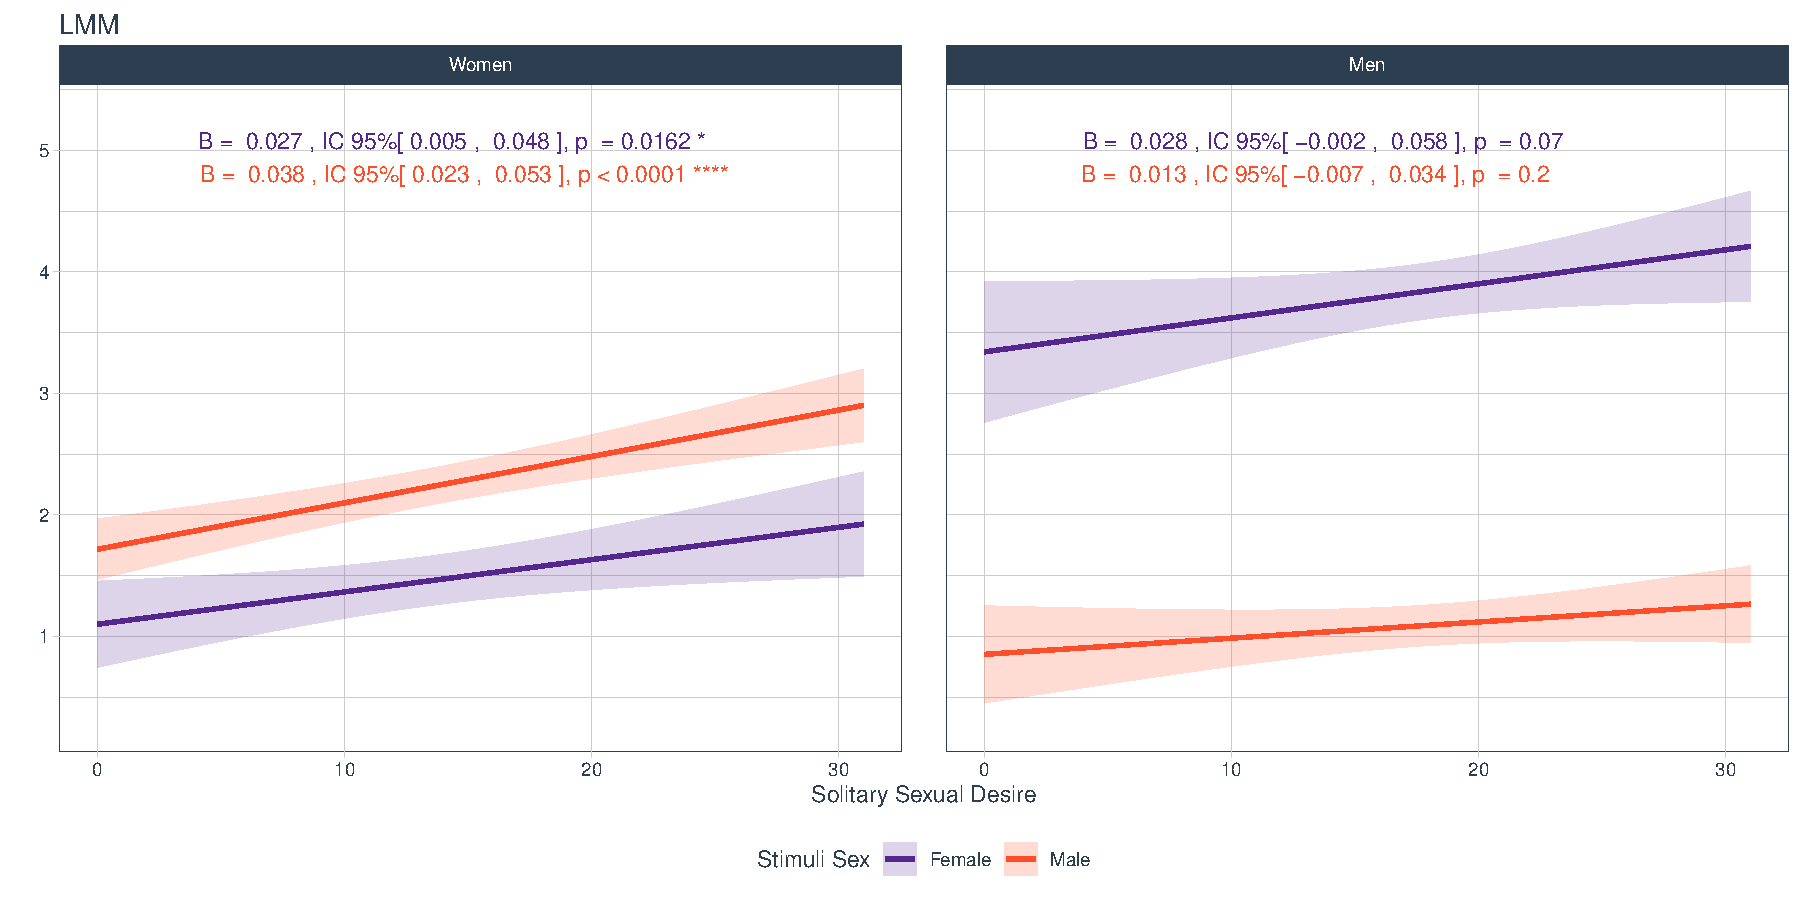
\includegraphics{Deseo_excitacion_sexual_files/figure-latex/fig-h2a-1.pdf}
\caption{\label{fig:fig-h2a}Subjective sexual arousal to erotic stimuli: Significant main effects and interactions of model 2A. For detailed results of the model, see Table \ref{tab:tab-m2a}. \textbf{(a)} Main effect of Solitary sexual desire on Subjective sexual arousal (for detailed results, see Table \ref{tab:tab-m2a}); \textbf{(b)} main effect of Dyadic sexual desire (Attractive person) on Subjective sexual arousal (for detailed results, see Table \ref{tab:tab-m2a}); \textbf{(c)} interaction between Stimuli sex and gender (significant effects of stimuli sex by participant gender are represented with lines and stars. White dots and black bars represent estimated marginal means and 95\% CI, calculated from 1000 bootstraped simulations; for detailed results, see Table \ref{tab:tab-m2a-emms-c}); \textbf{(d)} interaction between Stimuli sex and Dyadic sexual desire (Attractive person) (for detailed results, see Table \ref{tab:tab-m2a-slo-d}); \textbf{(e)} interaction between Stimuli sex, gender and Dyadic sexual desire (Attractive person) (for detailed results, see Table \ref{tab:tab-m2a-slo-e}); \textbf{(f)} interaction between Relationship, gender and Dyadic sexual desire (Partner) (for detailed results, see Table \ref{tab:tab-m2a-slo-f}); \textbf{(g)} interaction between Relationship, Stimuli sex and Dyadic sexual desire (Partner) (for detailed results, see Table \ref{tab:tab-m2a-slo-g}). \emph{Women} and \emph{Men} refer to the gender of the participants and \emph{Female} and \emph{Male} to the sex of the stimuli. To better represent the associations between predictor variables and subjective sexual arousal within the model (i.e.~when including all other effects), in all cases the \emph{Y} axis represents values predicted by the model instead of raw values. For statistical significance, *\emph{p} \textless{} 0.05, **\emph{p} \textless{} 0.01, ***\emph{p} \textless{} 0.001, ****\emph{p} \textless{} 0.0001.}
\end{figure}

\hypertarget{hypothesis2b}{%
\subsubsection{Hypothesis 2b: Non-erotic}\label{hypothesis2b}}

\hypertarget{filter-data-2}{%
\paragraph{Filter data}\label{filter-data-2}}

Create data frame selecting only relevant variables, and summarizing per sexual desire dimension for each participant (three rows per participant).

\begin{Shaded}
\begin{Highlighting}[]
\NormalTok{dat.nero }\OtherTok{\textless{}{-}}\NormalTok{ dat.fin }\SpecialCharTok{|\textgreater{}}
  \FunctionTok{filter}\NormalTok{(}\StringTok{\textasciigrave{}}\AttributeTok{Stimuli content}\StringTok{\textasciigrave{}} \SpecialCharTok{==} \StringTok{"Non{-}erotic"}\NormalTok{)}
\end{Highlighting}
\end{Shaded}

\hypertarget{fit-model-2}{%
\paragraph{Fit model}\label{fit-model-2}}

We modelled the effects of XXXXX.

\begin{Shaded}
\begin{Highlighting}[]
\FunctionTok{options}\NormalTok{(}\AttributeTok{contrasts =} \FunctionTok{c}\NormalTok{(}\StringTok{"contr.sum"}\NormalTok{,}\StringTok{"contr.poly"}\NormalTok{))}

\NormalTok{m2b }\OtherTok{\textless{}{-}} \FunctionTok{lmer}\NormalTok{(}\StringTok{\textasciigrave{}}\AttributeTok{Subjective sexual arousal}\StringTok{\textasciigrave{}} \SpecialCharTok{\textasciitilde{}}
\NormalTok{            Relationship }\SpecialCharTok{*}\NormalTok{ Gender }\SpecialCharTok{*} \StringTok{\textasciigrave{}}\AttributeTok{Stimuli sex}\StringTok{\textasciigrave{}} \SpecialCharTok{*} \StringTok{\textasciigrave{}}\AttributeTok{Solitary sexual desire (C)}\StringTok{\textasciigrave{}} \SpecialCharTok{+}
\NormalTok{            Relationship }\SpecialCharTok{*}\NormalTok{ Gender }\SpecialCharTok{*} \StringTok{\textasciigrave{}}\AttributeTok{Stimuli sex}\StringTok{\textasciigrave{}} \SpecialCharTok{*} \StringTok{\textasciigrave{}}\AttributeTok{Dyadic sexual desire (Attractive person) (C)}\StringTok{\textasciigrave{}} \SpecialCharTok{+}
\NormalTok{            Relationship }\SpecialCharTok{*}\NormalTok{ Gender }\SpecialCharTok{*} \StringTok{\textasciigrave{}}\AttributeTok{Stimuli sex}\StringTok{\textasciigrave{}} \SpecialCharTok{*} \StringTok{\textasciigrave{}}\AttributeTok{Dyadic sexual desire (Partner) (C)}\StringTok{\textasciigrave{}} \SpecialCharTok{+}
\NormalTok{            (}\DecValTok{1} \SpecialCharTok{|} \StringTok{\textasciigrave{}}\AttributeTok{Stimuli code}\StringTok{\textasciigrave{}}\NormalTok{) }\SpecialCharTok{+}
\NormalTok{            (}\DecValTok{1} \SpecialCharTok{+} \StringTok{\textasciigrave{}}\AttributeTok{Stimuli sex}\StringTok{\textasciigrave{}} \SpecialCharTok{|}\NormalTok{ Participant),}
           \AttributeTok{data =}\NormalTok{ dat.nero,}
           \AttributeTok{control =} \FunctionTok{lmerControl}\NormalTok{(}\AttributeTok{optimizer =} \StringTok{"bobyqa"}\NormalTok{))}
\end{Highlighting}
\end{Shaded}

\hypertarget{model-assumptions-2}{%
\subparagraph{Model assumptions}\label{model-assumptions-2}}

Most model assumptions were checked using the \texttt{check\_model} function from the \texttt{performance} package (\protect\hyperlink{ref-ludecke2021}{Lüdecke et al., 2021}), and reported in Fig. \ref{fig:assu-m2b}. These assumptions do not include collinearity, as the function plots \(VIF\) instead of the recommended Generalized Variance Inflation Factors (\(GVIF\)) and the most comparable \(GVIF^{{1}/{(2 \times df)}}\) (\protect\hyperlink{ref-fox1992}{Fox \& Monette, 1992}). Instead, \(GVIF\) and \(GVIF^{{1}/{(2 \times df)}}\) values are reported in Table \ref{tab:coli-m2b}.

Figure \ref{fig:assu-m2b}. Model assumptions

This figure includes most assumptions: linearity, homogeneity of variance, and normality of both residuals and random effects.

\begin{Shaded}
\begin{Highlighting}[]
\FunctionTok{check\_model}\NormalTok{(m2b,}
            \AttributeTok{check =} \FunctionTok{c}\NormalTok{(}\StringTok{"linearity"}\NormalTok{, }\StringTok{"homogeneity"}\NormalTok{, }\StringTok{"qq"}\NormalTok{, }\StringTok{"reqq"}\NormalTok{))}
\end{Highlighting}
\end{Shaded}

\begin{figure}
\centering
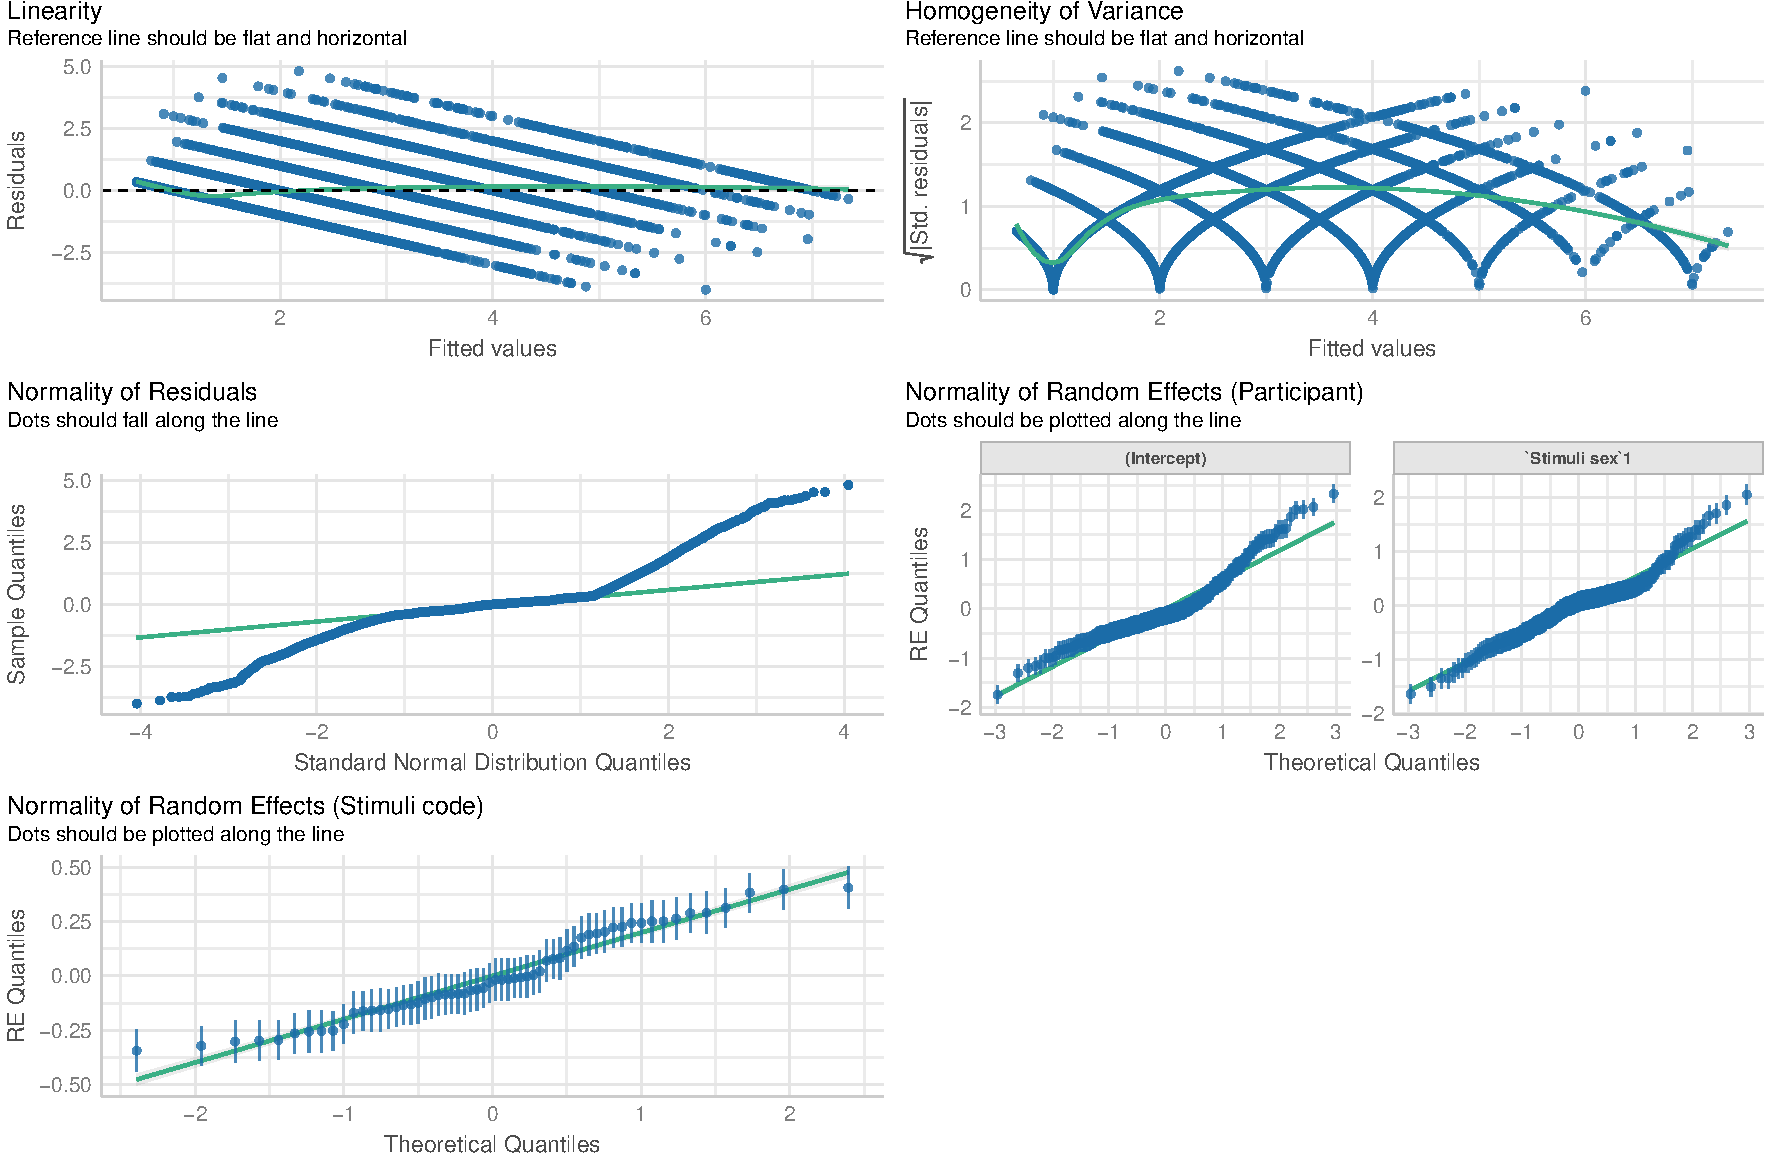
\includegraphics{Deseo_excitacion_sexual_files/figure-latex/assu-m2b-1.pdf}
\caption{\label{fig:assu-m2b}Model assumptions. Plots represent linearity, homogeneity of variance, and normality of both residuals and random effects (as QQ plots), respectively.}
\end{figure}

Table \ref{tab:coli-m2b}. Collinearity

Given the presence of interactions, that all predictors are categorical, and the absence of random slopes, \(VIF\) and \(GVIF\) values would be expected to be high.

\begin{Shaded}
\begin{Highlighting}[]
\FunctionTok{data.frame}\NormalTok{(}\FunctionTok{vif}\NormalTok{(m2b)) }\SpecialCharTok{|\textgreater{}} 
  \FunctionTok{rownames\_to\_column}\NormalTok{() }\SpecialCharTok{|\textgreater{}} 
  \FunctionTok{mutate\_at}\NormalTok{(}\StringTok{"rowname"}\NormalTok{, str\_replace\_all, }\StringTok{":"}\NormalTok{, }\StringTok{" × "}\NormalTok{) }\SpecialCharTok{|\textgreater{}}
  \FunctionTok{mutate\_at}\NormalTok{(}\StringTok{"rowname"}\NormalTok{, str\_replace\_all, }\StringTok{"\textasciigrave{}"}\NormalTok{, }\StringTok{""}\NormalTok{) }\SpecialCharTok{|\textgreater{}} 
  \FunctionTok{kable}\NormalTok{(}\AttributeTok{digits =} \DecValTok{2}\NormalTok{,}
        \AttributeTok{booktabs =} \ConstantTok{TRUE}\NormalTok{,}
        \AttributeTok{align =} \FunctionTok{c}\NormalTok{(}\StringTok{"l"}\NormalTok{, }\StringTok{"c"}\NormalTok{),}
        \AttributeTok{linesep =} \StringTok{""}\NormalTok{,}
        \AttributeTok{caption =} \StringTok{"Variance inflation factors for the model of hypothesis 2a"}\NormalTok{,}
        \AttributeTok{col.names =} \FunctionTok{c}\NormalTok{(}\StringTok{" "}\NormalTok{,}
                      \StringTok{"$VIF$"}\NormalTok{),}
        \AttributeTok{escape =} \ConstantTok{FALSE}\NormalTok{) }\SpecialCharTok{|\textgreater{}}
  \FunctionTok{kable\_styling}\NormalTok{(}\AttributeTok{latex\_options =} \StringTok{"HOLD\_position"}\NormalTok{)}
\end{Highlighting}
\end{Shaded}

\begin{table}[H]

\caption{\label{tab:coli-m2b}Variance inflation factors for the model of hypothesis 2a}
\centering
\begin{tabular}[t]{lc}
\toprule
  & $VIF$\\
\midrule
Relationship & 1.96\\
Gender & 1.95\\
Stimuli sex & 1.36\\
Solitary sexual desire (C) & 1.88\\
Dyadic sexual desire (Attractive person) (C) & 1.83\\
Dyadic sexual desire (Partner) (C) & 2.28\\
Relationship × Gender & 1.97\\
Relationship × Stimuli sex & 1.97\\
Gender × Stimuli sex & 1.96\\
Relationship × Solitary sexual desire (C) & 1.82\\
Gender × Solitary sexual desire (C) & 1.76\\
Stimuli sex × Solitary sexual desire (C) & 1.88\\
Relationship × Dyadic sexual desire (Attractive person) (C) & 1.77\\
Gender × Dyadic sexual desire (Attractive person) (C) & 1.65\\
Stimuli sex × Dyadic sexual desire (Attractive person) (C) & 1.83\\
Relationship × Dyadic sexual desire (Partner) (C) & 2.08\\
Gender × Dyadic sexual desire (Partner) (C) & 2.19\\
Stimuli sex × Dyadic sexual desire (Partner) (C) & 2.28\\
Relationship × Gender × Stimuli sex & 1.98\\
Relationship × Gender × Solitary sexual desire (C) & 1.84\\
Relationship × Stimuli sex × Solitary sexual desire (C) & 1.85\\
Gender × Stimuli sex × Solitary sexual desire (C) & 1.82\\
Relationship × Gender × Dyadic sexual desire (Attractive person) (C) & 1.81\\
Relationship × Stimuli sex × Dyadic sexual desire (Attractive person) (C) & 1.80\\
Gender × Stimuli sex × Dyadic sexual desire (Attractive person) (C) & 1.74\\
Relationship × Gender × Dyadic sexual desire (Partner) (C) & 2.28\\
Relationship × Stimuli sex × Dyadic sexual desire (Partner) (C) & 2.17\\
Gender × Stimuli sex × Dyadic sexual desire (Partner) (C) & 2.23\\
Relationship × Gender × Stimuli sex × Solitary sexual desire (C) & 1.86\\
Relationship × Gender × Stimuli sex × Dyadic sexual desire (Attractive person) (C) & 1.82\\
Relationship × Gender × Stimuli sex × Dyadic sexual desire (Partner) (C) & 2.28\\
\bottomrule
\end{tabular}
\end{table}

\hypertarget{bootstrap-confidence-intervals-1}{%
\subparagraph{Bootstrap confidence intervals}\label{bootstrap-confidence-intervals-1}}

\begin{Shaded}
\begin{Highlighting}[]
\NormalTok{m2bCI }\OtherTok{\textless{}{-}} \FunctionTok{confint}\NormalTok{(m2b, }
                 \AttributeTok{method =} \StringTok{"boot"}\NormalTok{, }\CommentTok{\#define bootstrap as the method for computing the confidence intervals}
                 \AttributeTok{nsim =} \DecValTok{4}\NormalTok{, }\CommentTok{\#number of simulations}
                 \AttributeTok{FUN =}\NormalTok{ fixef, }\CommentTok{\#to obtain only estimates for fixed effects}
                 \AttributeTok{parallel =} \StringTok{"multicore"}\NormalTok{, }\CommentTok{\#parallel computation}
                 \AttributeTok{ncpus =} \FunctionTok{detectCores}\NormalTok{()}\SpecialCharTok{{-}}\DecValTok{1}\NormalTok{, }\CommentTok{\#number of computational cores to run in parallel}
                 \AttributeTok{.progress =} \StringTok{"txt"}\NormalTok{, }\CommentTok{\#show progress bar}
                 \AttributeTok{seed =} \DecValTok{2023}\NormalTok{) }\CommentTok{\#to ensure reproducibility and allow cache to work}
\end{Highlighting}
\end{Shaded}

\begin{verbatim}
## ================================================================================
\end{verbatim}

\hypertarget{table-reftabtab-m2b.-regression-type-table-for-the-interaction-between-relationship-type-sexual-desire-dimension-and-gender}{%
\subparagraph{\texorpdfstring{Table \ref{tab:tab-m2b}. Regression-type table for the interaction between \texttt{Relationship\ type}, \texttt{Sexual\ desire\ dimension}, and \texttt{Gender}}{Table \ref{tab:tab-m2b}. Regression-type table for the interaction between Relationship type, Sexual desire dimension, and Gender}}\label{table-reftabtab-m2b.-regression-type-table-for-the-interaction-between-relationship-type-sexual-desire-dimension-and-gender}}

This tables summarizes the results of the model.

\begin{Shaded}
\begin{Highlighting}[]
\NormalTok{tab.m2b }\OtherTok{\textless{}{-}} \FunctionTok{summary.sig.boot}\NormalTok{(}\AttributeTok{mod =}\NormalTok{ m2b,}
                            \AttributeTok{modCI =}\NormalTok{ m2aCI, }
                            \AttributeTok{custom\_caption =} \StringTok{"Subjective sexual arousal in response to }
\StringTok{                            non{-}erotic stimuli, by relationship type, gender, stimuli sex, }
\StringTok{                            and the three dimensions of sexual desire dimension"}\NormalTok{)}
\NormalTok{tab.m2b}
\end{Highlighting}
\end{Shaded}

\begin{table}[H]

\caption{\label{tab:tab-m2b}Subjective sexual arousal in response to 
                            non-erotic stimuli, by relationship type, gender, stimuli sex, 
                            and the three dimensions of sexual desire dimension}
\centering
\resizebox{\linewidth}{!}{
\begin{threeparttable}
\begin{tabular}[t]{lccccccc}
\toprule
Effect & Estimate & Lower 95\% CI & Upper 95\% CI & Std. Error & $df$ & 
                        $t$ & $p$\\
\midrule
(Intercept) & 1.59 & 1.97 & 2.17 & 0.05 & 330.32 & 29.98 & \textbf{< 0.0001}\\
Relationship [Stable] & 0.02 & 0.04 & 0.06 & 0.05 & 304.00 & 0.49 & 0.63\\
Gender [Women] & -0.13 & -0.23 & -0.06 & 0.05 & 304.00 & -2.87 & \textbf{0.0043}\\
Stimuli sex [Female] & 0.19 & 0.43 & 0.51 & 0.05 & 302.42 & 3.89 & \textbf{< 0.001}\\
Solitary sexual desire (C) & 0.00 & 0.01 & 0.04 & 0.01 & 304.00 & 0.05 & 0.96\\
Dyadic sexual desire (Attractive person) (C) & 0.03 & 0.02 & 0.04 & 0.01 & 304.00 & 5.68 & \textbf{< 0.0001}\\
Dyadic sexual desire (Partner) (C) & 0.01 & -0.01 & 0.00 & 0.01 & 304.00 & 1.03 & 0.3\\
Relationship [Stable] × Gender [Women] & -0.01 & -0.09 & 0.07 & 0.05 & 304.00 & -0.29 & 0.77\\
Relationship [Stable] × Stimuli sex [Female] & 0.03 & -0.09 & 0.03 & 0.04 & 304.00 & 0.85 & 0.39\\
Gender [Women] × Stimuli sex [Female] & -0.49 & -0.90 & -0.68 & 0.04 & 304.00 & -12.14 & \textbf{< 0.0001}\\
Relationship [Stable] × Solitary sexual desire (C) & 0.00 & 0.00 & 0.00 & 0.01 & 304.00 & -0.39 & 0.69\\
Gender [Women] × Solitary sexual desire (C) & 0.01 & 0.00 & 0.01 & 0.01 & 304.00 & 2.49 & \textbf{0.0133}\\
Stimuli sex [Female] × Solitary sexual desire (C) & -0.01 & -0.01 & 0.00 & 0.00 & 304.00 & -2.03 & \textbf{0.0435}\\
Relationship [Stable] × Dyadic sexual desire (Attractive person) (C) & 0.00 & 0.00 & 0.01 & 0.01 & 304.00 & 0.28 & 0.78\\
Gender [Women] × Dyadic sexual desire (Attractive person) (C) & -0.02 & -0.01 & 0.00 & 0.01 & 304.00 & -2.90 & \textbf{0.004}\\
Stimuli sex [Female] × Dyadic sexual desire (Attractive person) (C) & 0.02 & 0.00 & 0.02 & 0.00 & 304.00 & 3.86 & \textbf{< 0.001}\\
Relationship [Stable] × Dyadic sexual desire (Partner) (C) & 0.00 & -0.01 & 0.01 & 0.01 & 304.00 & 0.07 & 0.94\\
Gender [Women] × Dyadic sexual desire (Partner) (C) & -0.01 & -0.01 & 0.00 & 0.01 & 304.00 & -1.44 & 0.15\\
Stimuli sex [Female] × Dyadic sexual desire (Partner) (C) & 0.01 & 0.01 & 0.01 & 0.00 & 304.00 & 1.10 & 0.27\\
Relationship [Stable] × Gender [Women] × Stimuli sex [Female] & 0.02 & -0.10 & 0.09 & 0.04 & 304.00 & 0.41 & 0.68\\
Relationship [Stable] × Gender [Women] × Solitary sexual desire (C) & 0.00 & 0.00 & 0.01 & 0.01 & 304.00 & 0.64 & 0.52\\
Relationship [Stable] × Stimuli sex [Female] × Solitary sexual desire (C) & 0.00 & 0.00 & 0.00 & 0.00 & 304.00 & 0.21 & 0.83\\
Gender [Women] × Stimuli sex [Female] × Solitary sexual desire (C) & 0.00 & -0.01 & 0.00 & 0.00 & 304.00 & 0.23 & 0.82\\
Relationship [Stable] × Gender [Women] × Dyadic sexual desire (Attractive person) (C) & 0.00 & -0.01 & 0.00 & 0.01 & 304.00 & -0.49 & 0.62\\
Relationship [Stable] × Stimuli sex [Female] × Dyadic sexual desire (Attractive person) (C) & 0.00 & 0.01 & 0.02 & 0.00 & 304.00 & 0.58 & 0.56\\
Gender [Women] × Stimuli sex [Female] × Dyadic sexual desire (Attractive person) (C) & -0.03 & -0.03 & -0.02 & 0.00 & 304.00 & -5.53 & \textbf{< 0.0001}\\
Relationship [Stable] × Gender [Women] × Dyadic sexual desire (Partner) (C) & 0.00 & 0.01 & 0.02 & 0.01 & 304.00 & 0.06 & 0.95\\
Relationship [Stable] × Stimuli sex [Female] × Dyadic sexual desire (Partner) (C) & 0.00 & -0.01 & -0.01 & 0.00 & 304.00 & -0.57 & 0.57\\
Gender [Women] × Stimuli sex [Female] × Dyadic sexual desire (Partner) (C) & -0.01 & -0.01 & 0.00 & 0.00 & 304.00 & -1.19 & 0.23\\
Relationship [Stable] × Gender [Women] × Stimuli sex [Female] × Solitary sexual desire (C) & 0.00 & 0.00 & 0.01 & 0.00 & 304.00 & 0.11 & 0.91\\
Relationship [Stable] × Gender [Women] × Stimuli sex [Female] × Dyadic sexual desire (Attractive person) (C) & 0.00 & -0.01 & 0.00 & 0.00 & 304.00 & 0.48 & 0.63\\
Relationship [Stable] × Gender [Women] × Stimuli sex [Female] × Dyadic sexual desire (Partner) (C) & 0.00 & -0.01 & 0.00 & 0.00 & 304.00 & -0.43 & 0.67\\
\bottomrule
\end{tabular}
\begin{tablenotes}[para]
\item \textit{Note: } 
\item $R^2_{conditional}$ = 0.722, $R^2_{marginal}$ = 0.292. Results are from linear mixed models for main 
                              effects and interactions between sexual desire (SD) dimensions,
                              sex, and Stimuli sex.
                              Confidence intervales were calculated as the 2.5 and 97.5 
                              percentiles from bootstrap (1000 simulations).
                              Continuous variables were centered and scaled
                              (represented as \textbf{(C)} in variable names).
                              Gender = participants gender (women, men); 
                              Stimuli sex = sex of stimuli (female, male); 
                              Solitary SD = Solitary Sexual Desire;
                              Attractive person DSD = Dyadic Sexual Desire toward an 
                              Attractive person;
                              Partner DSD = Dyadic Sexual Desire toward partner.
                              \textit{Sum-to-zero} contrasts were used to display
                              \textit{p}-values that represent main effects and interactions 
                              in an ANOVA-type manner (i.e. the intercept is the grand mean of 
                              all cells, and estimates are differences between each category
                              mean and the mean of all categories).
                              As reference categories 
                              \textit{Single} was used for relationship status,
                              \textit{Men} for gender,
                              and \textit{Male} for stimuli sex. 
                              Contrasted levels are in square brackets. 
                              Significant effects are in bold.
\end{tablenotes}
\end{threeparttable}}
\end{table}

\hypertarget{simple-slope-analysis-and-post-hoc-comparisons-1}{%
\subparagraph{\texorpdfstring{Simple slope analysis and \emph{post-hoc} comparisons}{Simple slope analysis and post-hoc comparisons}}\label{simple-slope-analysis-and-post-hoc-comparisons-1}}

We further explored the interaction between gender and stimuli sex using estimated marginal means, as well as comparing subjective sexual arousal between stimuli sex for each participant gender.

Table \ref{tab:tab-m2b-emms-b}. Estimated marginal means and contrasts of subjective arousal between stimuli sex by participant gender

Table of estimated marginal means and contrasts between stimuli sex for each participant gender. All estimated marginal means and contrasts were calculated using the \texttt{emmeans} function from the \texttt{emmeans} package (\protect\hyperlink{ref-emmeanscit}{Lenth, 2022}).

\begin{Shaded}
\begin{Highlighting}[]
\NormalTok{emms.m2b\_b }\OtherTok{\textless{}{-}} \FunctionTok{emmeans}\NormalTok{(m2b, }\SpecialCharTok{\textasciitilde{}} \FunctionTok{factor}\NormalTok{(}\StringTok{\textasciigrave{}}\AttributeTok{Stimuli sex}\StringTok{\textasciigrave{}}\NormalTok{) }\SpecialCharTok{|}\NormalTok{ Gender,}
                    \AttributeTok{adjust =} \StringTok{"bonferroni"}\NormalTok{) }\CommentTok{\#asymptotic degrees of freedom}

\NormalTok{emms.m2b\_b.tab }\OtherTok{\textless{}{-}} \FunctionTok{tibble}\NormalTok{(}\FunctionTok{data.frame}\NormalTok{(emms.m2b\_b)) }\SpecialCharTok{|\textgreater{}}
  \FunctionTok{rename}\NormalTok{(}\StringTok{"Stimuli sex"} \OtherTok{=}\NormalTok{ Stimuli.sex) }\SpecialCharTok{|\textgreater{}} 
  \FunctionTok{mutate}\NormalTok{(}\StringTok{"Subjective sexual arousal (p)"} \OtherTok{=}\NormalTok{ emmean)}

\NormalTok{t.m2b\_b }\OtherTok{\textless{}{-}} \FunctionTok{contr.stars}\NormalTok{(emms.m2b\_b) }\SpecialCharTok{|\textgreater{}} 
  \FunctionTok{mutate}\NormalTok{(}\AttributeTok{p.value =} \FunctionTok{pval.lev}\NormalTok{(p.value))}

\NormalTok{t.m2b\_b.f }\OtherTok{\textless{}{-}}\NormalTok{ t.m2b\_b }\SpecialCharTok{|\textgreater{}} 
  \FunctionTok{insertRows}\NormalTok{(}\DecValTok{2}\NormalTok{, }\AttributeTok{new =} \ConstantTok{NA}\NormalTok{)}

\FunctionTok{merge}\NormalTok{(emms.m2b\_b.tab, t.m2b\_b.f, }\AttributeTok{by =} \DecValTok{0}\NormalTok{, }\AttributeTok{all =} \ConstantTok{TRUE}\NormalTok{) }\SpecialCharTok{|\textgreater{}}
  \FunctionTok{select}\NormalTok{(}\SpecialCharTok{{-}}\FunctionTok{c}\NormalTok{(}\DecValTok{1}\NormalTok{,}\DecValTok{3}\NormalTok{,}\DecValTok{6}\NormalTok{,}\DecValTok{9}\NormalTok{,}\DecValTok{12}\NormalTok{,}\DecValTok{15}\NormalTok{,}\DecValTok{18}\NormalTok{)) }\SpecialCharTok{|\textgreater{}} 
  \FunctionTok{unite}\NormalTok{(Contrast, group1, group2, }\AttributeTok{sep =} \StringTok{" {-} "}\NormalTok{) }\SpecialCharTok{|\textgreater{}}
  \FunctionTok{mutate\_at}\NormalTok{(}\StringTok{"Contrast"}\NormalTok{, str\_replace\_all, }\StringTok{"NA {-} NA"}\NormalTok{, }\StringTok{" "}\NormalTok{) }\SpecialCharTok{|\textgreater{}} 
  \FunctionTok{kable}\NormalTok{(}\AttributeTok{digits =} \DecValTok{2}\NormalTok{,}
          \AttributeTok{booktabs =} \ConstantTok{TRUE}\NormalTok{,}
          \AttributeTok{align =} \FunctionTok{c}\NormalTok{(}\StringTok{"l"}\NormalTok{, }\FunctionTok{rep}\NormalTok{(}\StringTok{"c"}\NormalTok{, }\DecValTok{5}\NormalTok{), }\StringTok{"l"}\NormalTok{, }\FunctionTok{rep}\NormalTok{(}\StringTok{"c"}\NormalTok{, }\DecValTok{5}\NormalTok{)),}
          \AttributeTok{linesep =} \StringTok{""}\NormalTok{,}
          \AttributeTok{caption =} \StringTok{"Estimated marginal means of subjective sexual arousal for gender by}
\StringTok{        stimuli sex, in response to non{-}erotic stimuli"}\NormalTok{,}
          \AttributeTok{col.names =} \FunctionTok{c}\NormalTok{(}\StringTok{"Stimuli sex"}\NormalTok{,}
                        \StringTok{"EMM"}\NormalTok{,}
                        \StringTok{"$SE$"}\NormalTok{,}
                        \StringTok{"$2.5}\SpecialCharTok{\textbackslash{}\textbackslash{}}\StringTok{\% CI$"}\NormalTok{,}
                        \StringTok{"$97.5}\SpecialCharTok{\textbackslash{}\textbackslash{}}\StringTok{\% CI$"}\NormalTok{,}
                        \StringTok{"Contrast"}\NormalTok{,}
                        \StringTok{"Difference"}\NormalTok{,}
                        \StringTok{"$SE$"}\NormalTok{,}
                        \StringTok{"$z$"}\NormalTok{,}
                        \StringTok{"$p$"}\NormalTok{),}
          \AttributeTok{escape =} \ConstantTok{FALSE}\NormalTok{) }\SpecialCharTok{|\textgreater{}}
  \FunctionTok{pack\_rows}\NormalTok{(}\AttributeTok{group\_label =} \StringTok{"Women"}\NormalTok{,}
            \AttributeTok{start\_row =} \DecValTok{1}\NormalTok{,}
            \AttributeTok{end\_row =} \DecValTok{2}\NormalTok{,}
            \AttributeTok{bold =} \ConstantTok{TRUE}\NormalTok{) }\SpecialCharTok{|\textgreater{}}
  \FunctionTok{pack\_rows}\NormalTok{(}\AttributeTok{group\_label =} \StringTok{"Men"}\NormalTok{,}
            \AttributeTok{start\_row =} \DecValTok{3}\NormalTok{,}
            \AttributeTok{end\_row =} \DecValTok{4}\NormalTok{,}
            \AttributeTok{hline\_before =} \ConstantTok{TRUE}\NormalTok{,}
            \AttributeTok{bold =} \ConstantTok{TRUE}\NormalTok{) }\SpecialCharTok{|\textgreater{}}
  \FunctionTok{add\_header\_above}\NormalTok{(}\FunctionTok{c}\NormalTok{(}\StringTok{" "} \OtherTok{=} \DecValTok{5}\NormalTok{, }\StringTok{"Contrasts"} \OtherTok{=} \DecValTok{5}\NormalTok{)) }\SpecialCharTok{|\textgreater{}} 
  \FunctionTok{kable\_styling}\NormalTok{(}\AttributeTok{latex\_options =} \FunctionTok{c}\NormalTok{(}\StringTok{"HOLD\_position"}\NormalTok{, }\StringTok{"scale\_down"}\NormalTok{)) }\SpecialCharTok{|\textgreater{}}
  \FunctionTok{footnote}\NormalTok{(}\AttributeTok{general =} \StringTok{"EMM = estimated marginal mean.}
\StringTok{           No degrees of freedom are reported, as an asymptotic method was used. }
\StringTok{           Because of this, }\SpecialCharTok{\textbackslash{}\textbackslash{}\textbackslash{}\textbackslash{}}\StringTok{textit\{z\} rather that }\SpecialCharTok{\textbackslash{}\textbackslash{}\textbackslash{}\textbackslash{}}\StringTok{textit\{t\} scores are reported.}
\StringTok{           Bonferroni adjustment was used."}\NormalTok{,}
           \AttributeTok{threeparttable =} \ConstantTok{TRUE}\NormalTok{,}
           \AttributeTok{footnote\_as\_chunk =} \ConstantTok{TRUE}\NormalTok{,}
           \AttributeTok{escape =} \ConstantTok{FALSE}\NormalTok{)}
\end{Highlighting}
\end{Shaded}

\begin{table}[H]

\caption{\label{tab:tab-m2b-emms-b}Estimated marginal means of subjective sexual arousal for gender by
        stimuli sex, in response to non-erotic stimuli}
\centering
\resizebox{\linewidth}{!}{
\begin{threeparttable}
\begin{tabular}[t]{lccccclccc}
\toprule
\multicolumn{5}{c}{ } & \multicolumn{5}{c}{Contrasts} \\
\cmidrule(l{3pt}r{3pt}){6-10}
Stimuli sex & EMM & $SE$ & $2.5\% CI$ & $97.5\% CI$ & Contrast & Difference & $SE$ & $z$ & $p$\\
\midrule
\addlinespace[0.3em]
\multicolumn{10}{l}{\textbf{Women}}\\
\hspace{1em}Female & 1.16 & 0.10 & 0.93 & 1.38 & Female - Male & -0.60 & 0.11 & -5.27 & \textbf{< 0.0001}\\
\hspace{1em}Male & 1.76 & 0.07 & 1.60 & 1.91 &  &  &  &  & \\
\addlinespace[0.3em]
\hline
\multicolumn{10}{l}{\textbf{Men}}\\
\hspace{1em}Female & 2.40 & 0.12 & 2.13 & 2.67 & Female - Male & 1.36 & 0.14 & 9.88 & \textbf{< 0.0001}\\
\hspace{1em}Male & 1.04 & 0.08 & 0.86 & 1.22 &  &  &  &  & \\
\bottomrule
\end{tabular}
\begin{tablenotes}[para]
\item \textit{Note: } 
\item EMM = estimated marginal mean.
           No degrees of freedom are reported, as an asymptotic method was used. 
           Because of this, \textit{z} rather that \textit{t} scores are reported.
           Bonferroni adjustment was used.
\end{tablenotes}
\end{threeparttable}}
\end{table}

Table \ref{tab:tab-m2b-slo-c}. Slope for Solitary sexual desire on Subjective sexual arousal by gender

Table of estimated slopes for Solitary sexual desire on Subjective sexual arousal for each gender from model 2b. Dyadic sexual desire (Attractive person) values were centered. Slopes were calculated using the \texttt{sim\_slopes} function from the \texttt{interactions} package (\protect\hyperlink{ref-interactionscit}{Long, 2019}).

\begin{Shaded}
\begin{Highlighting}[]
\NormalTok{slop.m2b\_c }\OtherTok{\textless{}{-}} \FunctionTok{sim\_slopes}\NormalTok{(m2b,}
                         \AttributeTok{pred =} \StringTok{"Solitary sexual desire (C)"}\NormalTok{, }
                         \AttributeTok{modx =} \StringTok{"Gender"}\NormalTok{)}

\NormalTok{slop.m2b\_c.tab }\OtherTok{\textless{}{-}} \FunctionTok{data.frame}\NormalTok{(slop.m2b\_c}\SpecialCharTok{$}\NormalTok{slopes) }\SpecialCharTok{|\textgreater{}}
  \FunctionTok{select}\NormalTok{(}\DecValTok{1}\NormalTok{,}\DecValTok{2}\NormalTok{,}\DecValTok{4}\NormalTok{,}\DecValTok{5}\SpecialCharTok{:}\DecValTok{7}\NormalTok{) }\SpecialCharTok{|\textgreater{}}
  \FunctionTok{mutate}\NormalTok{(}\FunctionTok{across}\NormalTok{(}\DecValTok{2}\SpecialCharTok{:}\DecValTok{6}\NormalTok{, as.numeric)) }\SpecialCharTok{|\textgreater{}}
  \FunctionTok{mutate}\NormalTok{(}\FunctionTok{across}\NormalTok{(}\DecValTok{2}\SpecialCharTok{:}\DecValTok{5}\NormalTok{, round, }\DecValTok{3}\NormalTok{)) }\SpecialCharTok{|\textgreater{}}
  \FunctionTok{mutate}\NormalTok{(}\AttributeTok{sig =} \FunctionTok{pval.stars}\NormalTok{(p)) }\SpecialCharTok{|\textgreater{}}
  \FunctionTok{rename}\NormalTok{(}\StringTok{"Gender"} \OtherTok{=} \StringTok{"Value.of.Gender"}\NormalTok{) }\SpecialCharTok{|\textgreater{}}
  \FunctionTok{rename}\NormalTok{(}\AttributeTok{Coefficient =}\NormalTok{ Est.)}

\NormalTok{slop.m2b\_c.tab[,}\SpecialCharTok{{-}}\FunctionTok{c}\NormalTok{(}\DecValTok{7}\NormalTok{)] }\SpecialCharTok{|\textgreater{}} 
  \FunctionTok{mutate}\NormalTok{(}\AttributeTok{p =} \FunctionTok{pval.lev}\NormalTok{(p)) }\SpecialCharTok{|\textgreater{}} 
  \FunctionTok{kable}\NormalTok{(}\AttributeTok{booktabs =} \ConstantTok{TRUE}\NormalTok{,}
        \AttributeTok{align =} \FunctionTok{c}\NormalTok{(}\StringTok{"l"}\NormalTok{, }\FunctionTok{rep}\NormalTok{(}\StringTok{"c"}\NormalTok{, }\DecValTok{5}\NormalTok{)),}
        \AttributeTok{caption =} \StringTok{"Slope for Solitary sexual desire on Subjective sexual arousal by gender"}\NormalTok{,}
        \AttributeTok{col.names =} \FunctionTok{c}\NormalTok{(}\StringTok{"Gender"}\NormalTok{,}
                      \StringTok{"$B$"}\NormalTok{,}
                      \StringTok{"$2.5}\SpecialCharTok{\textbackslash{}\textbackslash{}}\StringTok{\% CI$"}\NormalTok{,}
                      \StringTok{"$97.5}\SpecialCharTok{\textbackslash{}\textbackslash{}}\StringTok{\% CI$"}\NormalTok{,}
                      \StringTok{"$t$"}\NormalTok{,}
                      \StringTok{"$p$"}\NormalTok{),}
        \AttributeTok{escape =} \ConstantTok{FALSE}\NormalTok{) }\SpecialCharTok{|\textgreater{}} 
  \FunctionTok{kable\_styling}\NormalTok{(}\AttributeTok{latex\_options =} \FunctionTok{c}\NormalTok{(}\StringTok{"HOLD\_position"}\NormalTok{)) }\SpecialCharTok{|\textgreater{}}
  \FunctionTok{footnote}\NormalTok{(}\AttributeTok{general =} \StringTok{"$B$ and $CIs$ are for unstandardized coefficient.}
\StringTok{           No intercept is reported as continuous predictors were centered}
\StringTok{           and are dependent on this specific sample."}\NormalTok{,}
           \AttributeTok{threeparttable =} \ConstantTok{TRUE}\NormalTok{,}
           \AttributeTok{footnote\_as\_chunk =} \ConstantTok{TRUE}\NormalTok{,}
           \AttributeTok{escape =} \ConstantTok{FALSE}\NormalTok{)}
\end{Highlighting}
\end{Shaded}

\begin{table}[H]

\caption{\label{tab:tab-m2b-slo-c}Slope for Solitary sexual desire on Subjective sexual arousal by gender}
\centering
\begin{threeparttable}
\begin{tabular}[t]{lccccc}
\toprule
Gender & $B$ & $2.5\% CI$ & $97.5\% CI$ & $t$ & $p$\\
\midrule
Men & -0.013 & -0.028 & 0.003 & -1.628 & 0.10\\
Women & 0.013 & 0.000 & 0.027 & 1.917 & 0.06\\
\bottomrule
\end{tabular}
\begin{tablenotes}[para]
\item \textit{Note: } 
\item $B$ and $CIs$ are for unstandardized coefficient.
           No intercept is reported as continuous predictors were centered
           and are dependent on this specific sample.
\end{tablenotes}
\end{threeparttable}
\end{table}

Table \ref{tab:tab-m2b-slo-d}. Slope for Solitary sexual desire on Subjective sexual arousal by stimuli sex

Table of estimated slopes for Solitary sexual desire on Subjective sexual arousal for each stimuli sex from model 2b. Dyadic sexual desire (Attractive person) values were centered. Slopes were calculated using the \texttt{sim\_slopes} function from the \texttt{interactions} package (\protect\hyperlink{ref-interactionscit}{Long, 2019}).

\begin{Shaded}
\begin{Highlighting}[]
\NormalTok{slop.m2b\_d }\OtherTok{\textless{}{-}} \FunctionTok{sim\_slopes}\NormalTok{(m2b,}
                         \AttributeTok{pred =} \StringTok{"Solitary sexual desire (C)"}\NormalTok{, }
                         \AttributeTok{modx =} \StringTok{"Stimuli sex"}\NormalTok{)}

\NormalTok{slop.m2b\_d.tab }\OtherTok{\textless{}{-}} \FunctionTok{data.frame}\NormalTok{(slop.m2b\_d}\SpecialCharTok{$}\NormalTok{slopes) }\SpecialCharTok{|\textgreater{}}
  \FunctionTok{select}\NormalTok{(}\DecValTok{1}\NormalTok{,}\DecValTok{2}\NormalTok{,}\DecValTok{4}\NormalTok{,}\DecValTok{5}\SpecialCharTok{:}\DecValTok{7}\NormalTok{) }\SpecialCharTok{|\textgreater{}}
  \FunctionTok{mutate}\NormalTok{(}\FunctionTok{across}\NormalTok{(}\DecValTok{2}\SpecialCharTok{:}\DecValTok{6}\NormalTok{, as.numeric)) }\SpecialCharTok{|\textgreater{}}
  \FunctionTok{mutate}\NormalTok{(}\FunctionTok{across}\NormalTok{(}\DecValTok{2}\SpecialCharTok{:}\DecValTok{5}\NormalTok{, round, }\DecValTok{3}\NormalTok{)) }\SpecialCharTok{|\textgreater{}}
  \FunctionTok{mutate}\NormalTok{(}\AttributeTok{sig =} \FunctionTok{pval.stars}\NormalTok{(p)) }\SpecialCharTok{|\textgreater{}}
  \FunctionTok{rename}\NormalTok{(}\StringTok{"Stimuli sex"} \OtherTok{=} \StringTok{"Value.of.Stimuli.sex"}\NormalTok{) }\SpecialCharTok{|\textgreater{}}
  \FunctionTok{rename}\NormalTok{(}\AttributeTok{Coefficient =}\NormalTok{ Est.)}

\NormalTok{slop.m2b\_d.tab[,}\SpecialCharTok{{-}}\FunctionTok{c}\NormalTok{(}\DecValTok{7}\NormalTok{)] }\SpecialCharTok{|\textgreater{}} 
  \FunctionTok{mutate}\NormalTok{(}\AttributeTok{p =} \FunctionTok{pval.lev}\NormalTok{(p)) }\SpecialCharTok{|\textgreater{}} 
  \FunctionTok{kable}\NormalTok{(}\AttributeTok{booktabs =} \ConstantTok{TRUE}\NormalTok{,}
        \AttributeTok{align =} \FunctionTok{c}\NormalTok{(}\StringTok{"l"}\NormalTok{, }\FunctionTok{rep}\NormalTok{(}\StringTok{"c"}\NormalTok{, }\DecValTok{5}\NormalTok{)),}
        \AttributeTok{caption =} \StringTok{"Slope for Solitary sexual desire on Subjective sexual arousal by gender"}\NormalTok{,}
        \AttributeTok{col.names =} \FunctionTok{c}\NormalTok{(}\StringTok{"Stimuli sex"}\NormalTok{,}
                      \StringTok{"$B$"}\NormalTok{,}
                      \StringTok{"$2.5}\SpecialCharTok{\textbackslash{}\textbackslash{}}\StringTok{\% CI$"}\NormalTok{,}
                      \StringTok{"$97.5}\SpecialCharTok{\textbackslash{}\textbackslash{}}\StringTok{\% CI$"}\NormalTok{,}
                      \StringTok{"$t$"}\NormalTok{,}
                      \StringTok{"$p$"}\NormalTok{),}
        \AttributeTok{escape =} \ConstantTok{FALSE}\NormalTok{) }\SpecialCharTok{|\textgreater{}} 
  \FunctionTok{kable\_styling}\NormalTok{(}\AttributeTok{latex\_options =} \FunctionTok{c}\NormalTok{(}\StringTok{"HOLD\_position"}\NormalTok{)) }\SpecialCharTok{|\textgreater{}}
  \FunctionTok{footnote}\NormalTok{(}\AttributeTok{general =} \StringTok{"$B$ and $CIs$ are for unstandardized coefficient.}
\StringTok{           No intercept is reported as continuous predictors were centered}
\StringTok{           and are dependent on this specific sample."}\NormalTok{,}
           \AttributeTok{threeparttable =} \ConstantTok{TRUE}\NormalTok{,}
           \AttributeTok{footnote\_as\_chunk =} \ConstantTok{TRUE}\NormalTok{,}
           \AttributeTok{escape =} \ConstantTok{FALSE}\NormalTok{)}
\end{Highlighting}
\end{Shaded}

\begin{table}[H]

\caption{\label{tab:tab-m2b-slo-d}Slope for Solitary sexual desire on Subjective sexual arousal by gender}
\centering
\begin{threeparttable}
\begin{tabular}[t]{lccccc}
\toprule
Stimuli sex & $B$ & $2.5\% CI$ & $97.5\% CI$ & $t$ & $p$\\
\midrule
Male & 0.010 & -0.001 & 0.020 & 1.815 & 0.07\\
Female & -0.009 & -0.026 & 0.007 & -1.094 & 0.27\\
\bottomrule
\end{tabular}
\begin{tablenotes}[para]
\item \textit{Note: } 
\item $B$ and $CIs$ are for unstandardized coefficient.
           No intercept is reported as continuous predictors were centered
           and are dependent on this specific sample.
\end{tablenotes}
\end{threeparttable}
\end{table}

Table \ref{tab:tab-m2b-slo-e}. Slope for Dyadic sexual desire (Attractive person) on Subjective sexual arousal by stimuli sex and gender

Table of estimated slopes for Dyadic sexual desire (Attractive person) on Subjective sexual arousal for each stimuli sex and gender from model 2b. Dyadic sexual desire (Attractive person) values were centered. Slopes were calculated using the \texttt{sim\_slopes} function from the \texttt{interactions} package (\protect\hyperlink{ref-interactionscit}{Long, 2019}).

\begin{Shaded}
\begin{Highlighting}[]
\NormalTok{slop.m2b\_e }\OtherTok{\textless{}{-}} \FunctionTok{sim\_slopes}\NormalTok{(m2b, }
                         \AttributeTok{pred =} \StringTok{"Dyadic sexual desire (Attractive person) (C)"}\NormalTok{, }
                         \AttributeTok{mod2 =} \StringTok{"Gender"}\NormalTok{,}
                         \AttributeTok{modx =} \StringTok{"Stimuli sex"}\NormalTok{)}

\NormalTok{slop.m2b\_e.tab }\OtherTok{\textless{}{-}} \FunctionTok{rbind}\NormalTok{(}\FunctionTok{data.frame}\NormalTok{(slop.m2b\_e}\SpecialCharTok{$}\NormalTok{slopes[}\DecValTok{1}\NormalTok{]),}
                        \FunctionTok{data.frame}\NormalTok{(slop.m2b\_e}\SpecialCharTok{$}\NormalTok{slopes[}\DecValTok{2}\NormalTok{])) }\SpecialCharTok{|\textgreater{}}
  \FunctionTok{select}\NormalTok{(}\DecValTok{1}\NormalTok{,}\DecValTok{2}\NormalTok{,}\DecValTok{4}\NormalTok{,}\DecValTok{5}\SpecialCharTok{:}\DecValTok{7}\NormalTok{) }\SpecialCharTok{|\textgreater{}}
  \FunctionTok{mutate}\NormalTok{(}\FunctionTok{across}\NormalTok{(}\DecValTok{2}\SpecialCharTok{:}\DecValTok{6}\NormalTok{, as.numeric)) }\SpecialCharTok{|\textgreater{}}
  \FunctionTok{mutate}\NormalTok{(}\FunctionTok{across}\NormalTok{(}\DecValTok{2}\SpecialCharTok{:}\DecValTok{5}\NormalTok{, round, }\DecValTok{3}\NormalTok{)) }\SpecialCharTok{|\textgreater{}}
  \FunctionTok{mutate}\NormalTok{(}\AttributeTok{sig =} \FunctionTok{pval.stars}\NormalTok{(p)) }\SpecialCharTok{|\textgreater{}} 
  \FunctionTok{rename}\NormalTok{(}\StringTok{"Stimuli sex"} \OtherTok{=} \StringTok{"Value.of.Stimuli.sex"}\NormalTok{) }\SpecialCharTok{|\textgreater{}}
  \FunctionTok{rename}\NormalTok{(}\AttributeTok{Coefficient =}\NormalTok{ Est.) }\SpecialCharTok{|\textgreater{}} 
  \FunctionTok{mutate}\NormalTok{(}\AttributeTok{Gender =} \FunctionTok{rep}\NormalTok{(}\FunctionTok{c}\NormalTok{(}\StringTok{"Women"}\NormalTok{, }\StringTok{"Men"}\NormalTok{), }\AttributeTok{each =} \DecValTok{2}\NormalTok{)) }\SpecialCharTok{|\textgreater{}}
  \FunctionTok{select}\NormalTok{(}\DecValTok{8}\NormalTok{,}\DecValTok{1}\SpecialCharTok{:}\DecValTok{7}\NormalTok{)}

\NormalTok{slop.m2b\_e.tab[,}\SpecialCharTok{{-}}\FunctionTok{c}\NormalTok{(}\DecValTok{8}\NormalTok{)] }\SpecialCharTok{|\textgreater{}} 
  \FunctionTok{mutate}\NormalTok{(}\AttributeTok{p =} \FunctionTok{pval.lev}\NormalTok{(p)) }\SpecialCharTok{|\textgreater{}} 
  \FunctionTok{kable}\NormalTok{(}\AttributeTok{booktabs =} \ConstantTok{TRUE}\NormalTok{,}
        \AttributeTok{align =} \FunctionTok{c}\NormalTok{(}\StringTok{"l"}\NormalTok{, }\StringTok{"l"}\NormalTok{, }\FunctionTok{rep}\NormalTok{(}\StringTok{"c"}\NormalTok{, }\DecValTok{4}\NormalTok{)),}
        \AttributeTok{caption =} \StringTok{"Slope for Dyadic sexual desire (Attractive person) on }
\StringTok{        Subjective sexual arousal by stimuli sex and gender"}\NormalTok{,}
        \AttributeTok{col.names =} \FunctionTok{c}\NormalTok{(}\StringTok{"Gender"}\NormalTok{,}
                      \StringTok{"Stimuli sex"}\NormalTok{,}
                      \StringTok{"$B$"}\NormalTok{,}
                      \StringTok{"$2.5}\SpecialCharTok{\textbackslash{}\textbackslash{}}\StringTok{\% CI$"}\NormalTok{,}
                      \StringTok{"$97.5}\SpecialCharTok{\textbackslash{}\textbackslash{}}\StringTok{\% CI$"}\NormalTok{,}
                      \StringTok{"$t$"}\NormalTok{,}
                      \StringTok{"$p$"}\NormalTok{),}
        \AttributeTok{escape =} \ConstantTok{FALSE}\NormalTok{) }\SpecialCharTok{|\textgreater{}} 
  \FunctionTok{collapse\_rows}\NormalTok{(}\AttributeTok{columns =} \DecValTok{1}\NormalTok{, }\AttributeTok{valign =} \StringTok{"middle"}\NormalTok{) }\SpecialCharTok{|\textgreater{}} 
  \FunctionTok{kable\_styling}\NormalTok{(}\AttributeTok{latex\_options =} \FunctionTok{c}\NormalTok{(}\StringTok{"HOLD\_position"}\NormalTok{)) }\SpecialCharTok{|\textgreater{}}
  \FunctionTok{footnote}\NormalTok{(}\AttributeTok{general =} \StringTok{"$B$ and $CIs$ are for unstandardized coefficient.}
\StringTok{           No intercept is reported as continuous predictors were centered}
\StringTok{           and are dependent on this specific sample."}\NormalTok{,}
           \AttributeTok{threeparttable =} \ConstantTok{TRUE}\NormalTok{,}
           \AttributeTok{footnote\_as\_chunk =} \ConstantTok{TRUE}\NormalTok{,}
           \AttributeTok{escape =} \ConstantTok{FALSE}\NormalTok{)}
\end{Highlighting}
\end{Shaded}

\begin{table}[H]

\caption{\label{tab:tab-m2b-slo-e}Slope for Dyadic sexual desire (Attractive person) on 
        Subjective sexual arousal by stimuli sex and gender}
\centering
\begin{threeparttable}
\begin{tabular}[t]{llccccl}
\toprule
Gender & Stimuli sex & $B$ & $2.5\% CI$ & $97.5\% CI$ & $t$ & $p$\\
\midrule
 & Female & 0.007 & -0.015 & 0.029 & 0.656 & 0.51\\
\cmidrule{2-7}
\multirow{-2}{*}{\raggedright\arraybackslash Women} & Male & 0.024 & 0.010 & 0.038 & 3.327 & \textbf{< 0.001}\\
\cmidrule{1-7}
 & Female & 0.095 & 0.068 & 0.122 & 6.822 & \textbf{< 0.0001}\\
\cmidrule{2-7}
\multirow{-2}{*}{\raggedright\arraybackslash Men} & Male & 0.002 & -0.016 & 0.019 & 0.177 & 0.86\\
\bottomrule
\end{tabular}
\begin{tablenotes}[para]
\item \textit{Note: } 
\item $B$ and $CIs$ are for unstandardized coefficient.
           No intercept is reported as continuous predictors were centered
           and are dependent on this specific sample.
\end{tablenotes}
\end{threeparttable}
\end{table}

\hypertarget{figure-reffigfig-h2b.-subjective-sexual-arousal-to-non-erotic-stimuli-main-effects-and-interactions}{%
\paragraph{Figure \ref{fig:fig-h2b}. Subjective sexual arousal to non-erotic stimuli: Main effects and interactions}\label{figure-reffigfig-h2b.-subjective-sexual-arousal-to-non-erotic-stimuli-main-effects-and-interactions}}

This figure summarizes the results of hypothesis 2b.

\begin{Shaded}
\begin{Highlighting}[]
\DocumentationTok{\#\# Create data frame and add predicted values for plots}
\NormalTok{m2b.dat }\OtherTok{\textless{}{-}}\NormalTok{ m2b}\SpecialCharTok{@}\NormalTok{frame }\SpecialCharTok{|\textgreater{}} 
  \FunctionTok{mutate}\NormalTok{(}\StringTok{\textasciigrave{}}\AttributeTok{Subjective sexual arousal (p)}\StringTok{\textasciigrave{}} \OtherTok{=} \FunctionTok{predict}\NormalTok{(m2b))}

\DocumentationTok{\#\# Extract slope data from model summary for main effects of continuous predictors}
\NormalTok{slop.m2b\_a.tab }\OtherTok{\textless{}{-}} \FunctionTok{left\_join}\NormalTok{(}\FunctionTok{data.frame}\NormalTok{(}\FunctionTok{summary}\NormalTok{(m2b)}\SpecialCharTok{$}\NormalTok{coefficients) }\SpecialCharTok{|\textgreater{}}
                               \FunctionTok{rownames\_to\_column}\NormalTok{(),}
                             \FunctionTok{data.frame}\NormalTok{(m2bCI) }\SpecialCharTok{|\textgreater{}}
                               \FunctionTok{rownames\_to\_column}\NormalTok{(),}
                             \AttributeTok{by =} \StringTok{"rowname"}\NormalTok{) }\SpecialCharTok{|\textgreater{}}
  \FunctionTok{select}\NormalTok{(}\DecValTok{1}\SpecialCharTok{:}\DecValTok{2}\NormalTok{,}\DecValTok{7}\SpecialCharTok{:}\DecValTok{8}\NormalTok{,}\DecValTok{5}\SpecialCharTok{:}\DecValTok{6}\NormalTok{) }\SpecialCharTok{|\textgreater{}}
  \FunctionTok{mutate}\NormalTok{(}\FunctionTok{across}\NormalTok{(}\DecValTok{2}\SpecialCharTok{:}\DecValTok{5}\NormalTok{, round, }\DecValTok{3}\NormalTok{)) }\SpecialCharTok{|\textgreater{}}
  \FunctionTok{mutate}\NormalTok{(}\AttributeTok{Pr...t.. =} \FunctionTok{pval.lev2}\NormalTok{(Pr...t..))}

\CommentTok{\# \# Figure main effect of Dyadic sexual desire (Attractive person) on Subjective sexual arousal}
\NormalTok{p2b.a }\OtherTok{\textless{}{-}} \FunctionTok{ggplot}\NormalTok{(m2b.dat, }\FunctionTok{aes}\NormalTok{(}\AttributeTok{x =} \StringTok{\textasciigrave{}}\AttributeTok{Dyadic sexual desire (Attractive person) (C)}\StringTok{\textasciigrave{}}\NormalTok{, }
                             \AttributeTok{y =} \StringTok{\textasciigrave{}}\AttributeTok{Subjective sexual arousal (p)}\StringTok{\textasciigrave{}}\NormalTok{)) }\SpecialCharTok{+}
  \FunctionTok{geom\_jitter}\NormalTok{(}\AttributeTok{alpha =}  \FloatTok{0.01}\NormalTok{) }\SpecialCharTok{+}
  \FunctionTok{geom\_smooth}\NormalTok{(}\AttributeTok{method =} \StringTok{"lm"}\NormalTok{) }\SpecialCharTok{+}
  \FunctionTok{labs}\NormalTok{(}\AttributeTok{y =} \StringTok{"Subjective sexual}\SpecialCharTok{\textbackslash{}n}\StringTok{arousal (predicted)"}\NormalTok{) }\SpecialCharTok{+}
  \FunctionTok{geom\_text}\NormalTok{(}\AttributeTok{data =}\NormalTok{ slop.m2b\_a.tab[}\DecValTok{6}\NormalTok{,],}
            \AttributeTok{mapping =} \FunctionTok{aes}\NormalTok{(}\AttributeTok{x =} \SpecialCharTok{{-}}\ConstantTok{Inf}\NormalTok{, }\AttributeTok{y =}\ConstantTok{Inf}\NormalTok{,}
                          \AttributeTok{vjust =} \DecValTok{2}\NormalTok{, }\AttributeTok{hjust =} \SpecialCharTok{{-}}\FloatTok{0.03}\NormalTok{),}
            \AttributeTok{label =} \FunctionTok{paste}\NormalTok{(}\StringTok{"B = "}\NormalTok{, slop.m2b\_a.tab[}\DecValTok{6}\NormalTok{,]}\SpecialCharTok{$}\NormalTok{Estimate,}
                          \StringTok{", IC 95\%["}\NormalTok{,}
                          \FunctionTok{paste}\NormalTok{(slop.m2b\_a.tab[}\DecValTok{6}\NormalTok{,]}\SpecialCharTok{$}\NormalTok{X2.}\DecValTok{5}\NormalTok{..,}
\NormalTok{                                slop.m2b\_a.tab[}\DecValTok{6}\NormalTok{,]}\SpecialCharTok{$}\NormalTok{X97.}\DecValTok{5}\NormalTok{..,}
                                \AttributeTok{sep =} \StringTok{", "}\NormalTok{),}
                          \StringTok{"], p"}\NormalTok{, slop.m2b\_a.tab[}\DecValTok{6}\NormalTok{,]}\SpecialCharTok{$}\NormalTok{Pr...t.., }\StringTok{"****"}\NormalTok{),}
            \AttributeTok{size =} \DecValTok{3}\NormalTok{) }\SpecialCharTok{+}
  \FunctionTok{theme\_tq}\NormalTok{()}

\CommentTok{\# Figure interaction between Stimuli sex and gender}
\NormalTok{p2b.b }\OtherTok{\textless{}{-}} \FunctionTok{ggplot}\NormalTok{(m2b.dat, }\FunctionTok{aes}\NormalTok{(}\AttributeTok{x =} \StringTok{\textasciigrave{}}\AttributeTok{Stimuli sex}\StringTok{\textasciigrave{}}\NormalTok{, }
                             \AttributeTok{y =} \StringTok{\textasciigrave{}}\AttributeTok{Subjective sexual arousal (p)}\StringTok{\textasciigrave{}}\NormalTok{, }
                             \AttributeTok{color =} \StringTok{\textasciigrave{}}\AttributeTok{Stimuli sex}\StringTok{\textasciigrave{}}\NormalTok{)) }\SpecialCharTok{+}
  \FunctionTok{geom\_violin}\NormalTok{() }\SpecialCharTok{+}
  \FunctionTok{geom\_jitter}\NormalTok{(}\AttributeTok{alpha =} \FloatTok{0.01}\NormalTok{, }\AttributeTok{width =} \FloatTok{0.1}\NormalTok{) }\SpecialCharTok{+}
  \FunctionTok{scale\_color\_manual}\NormalTok{(}\AttributeTok{values =}\NormalTok{ color.StimuliSex) }\SpecialCharTok{+}
  \FunctionTok{scale\_fill\_manual}\NormalTok{(}\AttributeTok{values =}\NormalTok{ color.StimuliSex) }\SpecialCharTok{+}
  \FunctionTok{facet\_wrap}\NormalTok{(}\SpecialCharTok{\textasciitilde{}}\NormalTok{Gender) }\SpecialCharTok{+}
  \FunctionTok{geom\_errorbar}\NormalTok{(}\AttributeTok{data =}\NormalTok{ emms.m2b\_b.tab, }
                \AttributeTok{mapping =} \FunctionTok{aes}\NormalTok{(}\AttributeTok{ymin =}\NormalTok{ asymp.LCL, }\AttributeTok{ymax =}\NormalTok{ asymp.UCL), }
                \AttributeTok{colour =} \StringTok{"black"}\NormalTok{, }\AttributeTok{width =} \FloatTok{0.1}\NormalTok{) }\SpecialCharTok{+}
  \FunctionTok{geom\_point}\NormalTok{(}\AttributeTok{data =}\NormalTok{ emms.m2b\_b.tab, }
             \AttributeTok{shape =} \DecValTok{21}\NormalTok{, }\AttributeTok{size =} \DecValTok{3}\NormalTok{,}
             \AttributeTok{color =} \StringTok{"black"}\NormalTok{, }\AttributeTok{fill =} \StringTok{"white"}\NormalTok{) }\SpecialCharTok{+}
  \FunctionTok{stat\_pvalue\_manual}\NormalTok{(t.m2b\_b, }
                     \AttributeTok{label =} \StringTok{"p.signif"}\NormalTok{, }
                     \AttributeTok{y.position =} \FunctionTok{c}\NormalTok{(}\FloatTok{7.4}\NormalTok{,}\FloatTok{7.8}\NormalTok{), }
                     \AttributeTok{tip.length =} \DecValTok{0}\NormalTok{) }\SpecialCharTok{+}
  \FunctionTok{labs}\NormalTok{(}\AttributeTok{y =} \StringTok{" }\SpecialCharTok{\textbackslash{}n}\StringTok{ "}\NormalTok{)  }\SpecialCharTok{+}
  \FunctionTok{ylim}\NormalTok{(}\FunctionTok{c}\NormalTok{(}\DecValTok{0}\NormalTok{, }\FloatTok{8.5}\NormalTok{)) }\SpecialCharTok{+}
  \FunctionTok{theme\_tq}\NormalTok{() }\SpecialCharTok{+}
  \FunctionTok{theme}\NormalTok{(}\AttributeTok{legend.position =} \StringTok{"none"}\NormalTok{)}

\CommentTok{\# Figure interaction between gender and Solitary sexual desire}
\DocumentationTok{\#\# Extract data for by stimuli sex}
\NormalTok{slop.m2b\_c.tab\_wom }\OtherTok{\textless{}{-}} \FunctionTok{filter}\NormalTok{(slop.m2b\_c.tab, Gender }\SpecialCharTok{==} \StringTok{"Women"}\NormalTok{) }\SpecialCharTok{|\textgreater{}}
  \FunctionTok{mutate}\NormalTok{(}\AttributeTok{p =} \FunctionTok{pval.lev2}\NormalTok{(p))}
\NormalTok{slop.m2b\_c.tab\_men }\OtherTok{\textless{}{-}} \FunctionTok{filter}\NormalTok{(slop.m2b\_c.tab, Gender }\SpecialCharTok{==} \StringTok{"Men"}\NormalTok{) }\SpecialCharTok{|\textgreater{}}
  \FunctionTok{mutate}\NormalTok{(}\AttributeTok{p =} \FunctionTok{pval.lev2}\NormalTok{(p))}
\DocumentationTok{\#\# Plot}
\NormalTok{p2b.c }\OtherTok{\textless{}{-}} \FunctionTok{ggplot}\NormalTok{(m2b.dat, }\FunctionTok{aes}\NormalTok{(}\AttributeTok{x =} \StringTok{\textasciigrave{}}\AttributeTok{Solitary sexual desire (C)}\StringTok{\textasciigrave{}}\NormalTok{,}
                             \AttributeTok{y =} \StringTok{\textasciigrave{}}\AttributeTok{Subjective sexual arousal (p)}\StringTok{\textasciigrave{}}\NormalTok{,}
                             \AttributeTok{color =}\NormalTok{ Gender, }\AttributeTok{fill =}\NormalTok{ Gender)) }\SpecialCharTok{+}
  \FunctionTok{geom\_jitter}\NormalTok{(}\AttributeTok{alpha =} \FloatTok{0.01}\NormalTok{, }\AttributeTok{size =} \DecValTok{1}\NormalTok{, }\AttributeTok{width =} \FloatTok{0.4}\NormalTok{) }\SpecialCharTok{+}
  \FunctionTok{geom\_smooth}\NormalTok{(}\AttributeTok{method =} \StringTok{"lm"}\NormalTok{, }\AttributeTok{fullrange =} \ConstantTok{TRUE}\NormalTok{) }\SpecialCharTok{+}
  \FunctionTok{scale\_color\_manual}\NormalTok{(}\AttributeTok{values =}\NormalTok{ color.Gender) }\SpecialCharTok{+}
  \FunctionTok{scale\_fill\_manual}\NormalTok{(}\AttributeTok{values =}\NormalTok{ color.Gender) }\SpecialCharTok{+}
  \FunctionTok{geom\_text}\NormalTok{(}\AttributeTok{data =}\NormalTok{ slop.m2b\_c.tab\_wom,}
            \AttributeTok{mapping =} \FunctionTok{aes}\NormalTok{(}\AttributeTok{x =} \SpecialCharTok{{-}}\ConstantTok{Inf}\NormalTok{, }\AttributeTok{y =} \ConstantTok{Inf}\NormalTok{,}
            \AttributeTok{vjust =} \DecValTok{2}\NormalTok{, }\AttributeTok{hjust =} \SpecialCharTok{{-}}\FloatTok{0.03}\NormalTok{),}
            \AttributeTok{inherit.aes =} \ConstantTok{FALSE}\NormalTok{,}
            \AttributeTok{label =} \FunctionTok{paste}\NormalTok{(}\StringTok{"B = "}\NormalTok{, slop.m2b\_c.tab\_wom}\SpecialCharTok{$}\NormalTok{Coefficient, }
                          \StringTok{", IC 95\%["}\NormalTok{, }\FunctionTok{paste}\NormalTok{(slop.m2b\_c.tab\_wom}\SpecialCharTok{$}\NormalTok{X2.}\FloatTok{5.}\NormalTok{, }
\NormalTok{                                             slop.m2b\_c.tab\_wom}\SpecialCharTok{$}\NormalTok{X97.}\FloatTok{5.}\NormalTok{, }\AttributeTok{sep =} \StringTok{", "}\NormalTok{), }
                          \StringTok{"], p"}\NormalTok{, slop.m2b\_c.tab\_wom}\SpecialCharTok{$}\NormalTok{p, }
                          \FunctionTok{ifelse}\NormalTok{(}\FunctionTok{is.na}\NormalTok{(slop.m2b\_c.tab\_wom}\SpecialCharTok{$}\NormalTok{sig), }\StringTok{""}\NormalTok{, slop.m2b\_c.tab\_wom}\SpecialCharTok{$}\NormalTok{sig)),}
            \AttributeTok{color =}\NormalTok{ color.Gender[}\DecValTok{1}\NormalTok{], }\AttributeTok{size =} \DecValTok{3}\NormalTok{) }\SpecialCharTok{+}
  \FunctionTok{geom\_text}\NormalTok{(}\AttributeTok{data =}\NormalTok{ slop.m2b\_c.tab\_men,}
            \AttributeTok{mapping =} \FunctionTok{aes}\NormalTok{(}\AttributeTok{x =} \SpecialCharTok{{-}}\ConstantTok{Inf}\NormalTok{, }\AttributeTok{y =} \ConstantTok{Inf}\NormalTok{,}
            \AttributeTok{vjust =} \DecValTok{4}\NormalTok{, }\AttributeTok{hjust =} \SpecialCharTok{{-}}\FloatTok{0.03}\NormalTok{),}
            \AttributeTok{inherit.aes =} \ConstantTok{FALSE}\NormalTok{,}
            \AttributeTok{label =} \FunctionTok{paste}\NormalTok{(}\StringTok{"B = "}\NormalTok{, slop.m2b\_c.tab\_men}\SpecialCharTok{$}\NormalTok{Coefficient, }
                          \StringTok{", IC 95\%["}\NormalTok{, }\FunctionTok{paste}\NormalTok{(slop.m2b\_c.tab\_men}\SpecialCharTok{$}\NormalTok{X2.}\FloatTok{5.}\NormalTok{, }
\NormalTok{                                             slop.m2b\_c.tab\_men}\SpecialCharTok{$}\NormalTok{X97.}\FloatTok{5.}\NormalTok{, }\AttributeTok{sep =} \StringTok{", "}\NormalTok{), }
                          \StringTok{"], p"}\NormalTok{, slop.m2b\_c.tab\_men}\SpecialCharTok{$}\NormalTok{p, }
                          \FunctionTok{ifelse}\NormalTok{(}\FunctionTok{is.na}\NormalTok{(slop.m2b\_c.tab\_men}\SpecialCharTok{$}\NormalTok{sig), }\StringTok{""}\NormalTok{, slop.m2b\_c.tab\_men}\SpecialCharTok{$}\NormalTok{sig)),}
            \AttributeTok{color =}\NormalTok{ color.Gender[}\DecValTok{2}\NormalTok{], }\AttributeTok{size =} \DecValTok{3}\NormalTok{) }\SpecialCharTok{+}
  \FunctionTok{labs}\NormalTok{(}\AttributeTok{y =} \StringTok{"Subjective sexual}\SpecialCharTok{\textbackslash{}n}\StringTok{arousal (predicted)"}\NormalTok{) }\SpecialCharTok{+}
  \FunctionTok{theme\_tq}\NormalTok{()}

\CommentTok{\# Figure interaction between Stimuli sex and Solitary sexual desire}
\DocumentationTok{\#\# Extract data for by stimuli sex}
\NormalTok{slop.m2b\_d.tab\_f }\OtherTok{\textless{}{-}} \FunctionTok{filter}\NormalTok{(slop.m2b\_d.tab, }\StringTok{\textasciigrave{}}\AttributeTok{Stimuli sex}\StringTok{\textasciigrave{}} \SpecialCharTok{==} \StringTok{"Female"}\NormalTok{) }\SpecialCharTok{|\textgreater{}}
  \FunctionTok{mutate}\NormalTok{(}\AttributeTok{p =} \FunctionTok{pval.lev2}\NormalTok{(p))}
\NormalTok{slop.m2b\_d.tab\_m }\OtherTok{\textless{}{-}} \FunctionTok{filter}\NormalTok{(slop.m2b\_d.tab, }\StringTok{\textasciigrave{}}\AttributeTok{Stimuli sex}\StringTok{\textasciigrave{}} \SpecialCharTok{==} \StringTok{"Male"}\NormalTok{) }\SpecialCharTok{|\textgreater{}}
  \FunctionTok{mutate}\NormalTok{(}\AttributeTok{p =} \FunctionTok{pval.lev2}\NormalTok{(p))}
\DocumentationTok{\#\# Plot}
\NormalTok{p2b.d }\OtherTok{\textless{}{-}} \FunctionTok{ggplot}\NormalTok{(m2b.dat, }\FunctionTok{aes}\NormalTok{(}\AttributeTok{x =} \StringTok{\textasciigrave{}}\AttributeTok{Dyadic sexual desire (Attractive person) (C)}\StringTok{\textasciigrave{}}\NormalTok{,}
                             \AttributeTok{y =} \StringTok{\textasciigrave{}}\AttributeTok{Subjective sexual arousal (p)}\StringTok{\textasciigrave{}}\NormalTok{,}
                             \AttributeTok{color =} \StringTok{\textasciigrave{}}\AttributeTok{Stimuli sex}\StringTok{\textasciigrave{}}\NormalTok{, }\AttributeTok{fill =} \StringTok{\textasciigrave{}}\AttributeTok{Stimuli sex}\StringTok{\textasciigrave{}}\NormalTok{)) }\SpecialCharTok{+}
  \FunctionTok{geom\_jitter}\NormalTok{(}\AttributeTok{alpha =} \FloatTok{0.01}\NormalTok{, }\AttributeTok{size =} \DecValTok{1}\NormalTok{, }\AttributeTok{width =} \FloatTok{0.4}\NormalTok{) }\SpecialCharTok{+}
  \FunctionTok{geom\_smooth}\NormalTok{(}\AttributeTok{method =} \StringTok{"lm"}\NormalTok{, }\AttributeTok{fullrange =} \ConstantTok{TRUE}\NormalTok{) }\SpecialCharTok{+}
  \FunctionTok{scale\_color\_manual}\NormalTok{(}\AttributeTok{values =}\NormalTok{ color.StimuliSex) }\SpecialCharTok{+}
  \FunctionTok{scale\_fill\_manual}\NormalTok{(}\AttributeTok{values =}\NormalTok{ color.StimuliSex) }\SpecialCharTok{+}
  \FunctionTok{geom\_text}\NormalTok{(}\AttributeTok{data =}\NormalTok{ slop.m2b\_d.tab\_f,}
            \AttributeTok{mapping =} \FunctionTok{aes}\NormalTok{(}\AttributeTok{x =} \SpecialCharTok{{-}}\ConstantTok{Inf}\NormalTok{, }\AttributeTok{y =} \ConstantTok{Inf}\NormalTok{,}
            \AttributeTok{vjust =} \DecValTok{2}\NormalTok{, }\AttributeTok{hjust =} \SpecialCharTok{{-}}\FloatTok{0.03}\NormalTok{),}
            \AttributeTok{inherit.aes =} \ConstantTok{FALSE}\NormalTok{,}
            \AttributeTok{label =} \FunctionTok{paste}\NormalTok{(}\StringTok{"B = "}\NormalTok{, slop.m2b\_d.tab\_f}\SpecialCharTok{$}\NormalTok{Coefficient, }
                          \StringTok{", IC 95\%["}\NormalTok{, }\FunctionTok{paste}\NormalTok{(slop.m2b\_d.tab\_f}\SpecialCharTok{$}\NormalTok{X2.}\FloatTok{5.}\NormalTok{, }
\NormalTok{                                             slop.m2b\_d.tab\_f}\SpecialCharTok{$}\NormalTok{X97.}\FloatTok{5.}\NormalTok{, }\AttributeTok{sep =} \StringTok{", "}\NormalTok{), }
                          \StringTok{"], p"}\NormalTok{, slop.m2b\_d.tab\_f}\SpecialCharTok{$}\NormalTok{p, }
                          \FunctionTok{ifelse}\NormalTok{(}\FunctionTok{is.na}\NormalTok{(slop.m2b\_d.tab\_f}\SpecialCharTok{$}\NormalTok{sig), }\StringTok{""}\NormalTok{, slop.m2b\_d.tab\_f}\SpecialCharTok{$}\NormalTok{sig)),}
            \AttributeTok{color =}\NormalTok{ color.StimuliSex[}\DecValTok{1}\NormalTok{], }\AttributeTok{size =} \DecValTok{3}\NormalTok{) }\SpecialCharTok{+}
  \FunctionTok{geom\_text}\NormalTok{(}\AttributeTok{data =}\NormalTok{ slop.m2b\_d.tab\_m,}
            \AttributeTok{mapping =} \FunctionTok{aes}\NormalTok{(}\AttributeTok{x =} \SpecialCharTok{{-}}\ConstantTok{Inf}\NormalTok{, }\AttributeTok{y =} \ConstantTok{Inf}\NormalTok{,}
            \AttributeTok{vjust =} \DecValTok{4}\NormalTok{, }\AttributeTok{hjust =} \SpecialCharTok{{-}}\FloatTok{0.03}\NormalTok{),}
            \AttributeTok{inherit.aes =} \ConstantTok{FALSE}\NormalTok{,}
            \AttributeTok{label =} \FunctionTok{paste}\NormalTok{(}\StringTok{"B = "}\NormalTok{, slop.m2b\_d.tab\_m}\SpecialCharTok{$}\NormalTok{Coefficient, }
                          \StringTok{", IC 95\%["}\NormalTok{, }\FunctionTok{paste}\NormalTok{(slop.m2b\_d.tab\_m}\SpecialCharTok{$}\NormalTok{X2.}\FloatTok{5.}\NormalTok{, }
\NormalTok{                                             slop.m2b\_d.tab\_m}\SpecialCharTok{$}\NormalTok{X97.}\FloatTok{5.}\NormalTok{, }\AttributeTok{sep =} \StringTok{", "}\NormalTok{), }
                          \StringTok{"], p"}\NormalTok{, slop.m2b\_d.tab\_m}\SpecialCharTok{$}\NormalTok{p, }
                          \FunctionTok{ifelse}\NormalTok{(}\FunctionTok{is.na}\NormalTok{(slop.m2b\_d.tab\_m}\SpecialCharTok{$}\NormalTok{sig), }\StringTok{""}\NormalTok{, slop.m2b\_d.tab\_m}\SpecialCharTok{$}\NormalTok{sig)),}
            \AttributeTok{color =}\NormalTok{ color.StimuliSex[}\DecValTok{2}\NormalTok{], }\AttributeTok{size =} \DecValTok{3}\NormalTok{) }\SpecialCharTok{+}
  \FunctionTok{labs}\NormalTok{(}\AttributeTok{y =} \StringTok{" }\SpecialCharTok{\textbackslash{}n}\StringTok{ "}\NormalTok{) }\SpecialCharTok{+}
  \FunctionTok{theme\_tq}\NormalTok{()}

\CommentTok{\# Figure interaction between Stimuli sex, gender and Dyadic sexual desire (Attractive person)}
\DocumentationTok{\#\# Extract data for by stimuli sex}
\NormalTok{slop.m2b\_e.tab\_f }\OtherTok{\textless{}{-}} \FunctionTok{filter}\NormalTok{(slop.m2b\_e.tab, }\StringTok{\textasciigrave{}}\AttributeTok{Stimuli sex}\StringTok{\textasciigrave{}} \SpecialCharTok{==} \StringTok{"Female"}\NormalTok{) }\SpecialCharTok{|\textgreater{}}
  \FunctionTok{mutate}\NormalTok{(}\AttributeTok{p =} \FunctionTok{pval.lev2}\NormalTok{(p))}
\NormalTok{slop.m2b\_e.tab\_m }\OtherTok{\textless{}{-}} \FunctionTok{filter}\NormalTok{(slop.m2b\_e.tab, }\StringTok{\textasciigrave{}}\AttributeTok{Stimuli sex}\StringTok{\textasciigrave{}} \SpecialCharTok{==} \StringTok{"Male"}\NormalTok{) }\SpecialCharTok{|\textgreater{}}
  \FunctionTok{mutate}\NormalTok{(}\AttributeTok{p =} \FunctionTok{pval.lev2}\NormalTok{(p))}
\DocumentationTok{\#\# Plot}
\NormalTok{p2b.e }\OtherTok{\textless{}{-}} \FunctionTok{ggplot}\NormalTok{(m2b.dat, }\FunctionTok{aes}\NormalTok{(}\AttributeTok{x =} \StringTok{\textasciigrave{}}\AttributeTok{Dyadic sexual desire (Attractive person) (C)}\StringTok{\textasciigrave{}}\NormalTok{,}
                             \AttributeTok{y =} \StringTok{\textasciigrave{}}\AttributeTok{Subjective sexual arousal (p)}\StringTok{\textasciigrave{}}\NormalTok{,}
                             \AttributeTok{color =} \StringTok{\textasciigrave{}}\AttributeTok{Stimuli sex}\StringTok{\textasciigrave{}}\NormalTok{, }\AttributeTok{fill =} \StringTok{\textasciigrave{}}\AttributeTok{Stimuli sex}\StringTok{\textasciigrave{}}\NormalTok{)) }\SpecialCharTok{+}
  \FunctionTok{geom\_jitter}\NormalTok{(}\AttributeTok{alpha =} \FloatTok{0.01}\NormalTok{, }\AttributeTok{size =} \DecValTok{1}\NormalTok{, }\AttributeTok{width =} \FloatTok{0.4}\NormalTok{) }\SpecialCharTok{+}
  \FunctionTok{geom\_smooth}\NormalTok{(}\AttributeTok{method =} \StringTok{"lm"}\NormalTok{, }\AttributeTok{fullrange =} \ConstantTok{TRUE}\NormalTok{) }\SpecialCharTok{+}
  \FunctionTok{scale\_color\_manual}\NormalTok{(}\AttributeTok{values =}\NormalTok{ color.StimuliSex) }\SpecialCharTok{+}
  \FunctionTok{scale\_fill\_manual}\NormalTok{(}\AttributeTok{values =}\NormalTok{ color.StimuliSex) }\SpecialCharTok{+}
  \FunctionTok{facet\_wrap}\NormalTok{(}\SpecialCharTok{\textasciitilde{}}\FunctionTok{fct\_relevel}\NormalTok{(Gender, }\StringTok{"Women"}\NormalTok{, }\StringTok{"Men"}\NormalTok{)) }\SpecialCharTok{+}
  \FunctionTok{geom\_text}\NormalTok{(}\AttributeTok{data =}\NormalTok{ slop.m2b\_e.tab\_f,}
            \AttributeTok{mapping =} \FunctionTok{aes}\NormalTok{(}\AttributeTok{x =} \SpecialCharTok{{-}}\ConstantTok{Inf}\NormalTok{, }\AttributeTok{y =} \ConstantTok{Inf}\NormalTok{,}
            \AttributeTok{vjust =} \DecValTok{2}\NormalTok{, }\AttributeTok{hjust =} \SpecialCharTok{{-}}\FloatTok{0.03}\NormalTok{),}
            \AttributeTok{inherit.aes =} \ConstantTok{FALSE}\NormalTok{,}
            \AttributeTok{label =} \FunctionTok{paste}\NormalTok{(}\StringTok{"B = "}\NormalTok{, slop.m2b\_e.tab\_f}\SpecialCharTok{$}\NormalTok{Coefficient, }
                          \StringTok{", IC 95\%["}\NormalTok{, }\FunctionTok{paste}\NormalTok{(slop.m2b\_e.tab\_f}\SpecialCharTok{$}\NormalTok{X2.}\FloatTok{5.}\NormalTok{, }
\NormalTok{                                             slop.m2b\_e.tab\_f}\SpecialCharTok{$}\NormalTok{X97.}\FloatTok{5.}\NormalTok{, }\AttributeTok{sep =} \StringTok{", "}\NormalTok{), }
                          \StringTok{"], p"}\NormalTok{, slop.m2b\_e.tab\_f}\SpecialCharTok{$}\NormalTok{p, }
                          \FunctionTok{ifelse}\NormalTok{(}\FunctionTok{is.na}\NormalTok{(slop.m2b\_e.tab\_f}\SpecialCharTok{$}\NormalTok{sig), }\StringTok{""}\NormalTok{, slop.m2b\_e.tab\_f}\SpecialCharTok{$}\NormalTok{sig)),}
            \AttributeTok{color =}\NormalTok{ color.StimuliSex[}\DecValTok{1}\NormalTok{], }\AttributeTok{size =} \FloatTok{2.5}\NormalTok{) }\SpecialCharTok{+}
  \FunctionTok{geom\_text}\NormalTok{(}\AttributeTok{data =}\NormalTok{ slop.m2b\_e.tab\_m,}
            \AttributeTok{mapping =} \FunctionTok{aes}\NormalTok{(}\AttributeTok{x =} \SpecialCharTok{{-}}\ConstantTok{Inf}\NormalTok{, }\AttributeTok{y =} \ConstantTok{Inf}\NormalTok{,}
            \AttributeTok{vjust =} \DecValTok{4}\NormalTok{, }\AttributeTok{hjust =} \SpecialCharTok{{-}}\FloatTok{0.03}\NormalTok{),}
            \AttributeTok{inherit.aes =} \ConstantTok{FALSE}\NormalTok{,}
            \AttributeTok{label =} \FunctionTok{paste}\NormalTok{(}\StringTok{"B = "}\NormalTok{, slop.m2b\_e.tab\_m}\SpecialCharTok{$}\NormalTok{Coefficient, }
                          \StringTok{", IC 95\%["}\NormalTok{, }\FunctionTok{paste}\NormalTok{(slop.m2b\_e.tab\_m}\SpecialCharTok{$}\NormalTok{X2.}\FloatTok{5.}\NormalTok{, }
\NormalTok{                                             slop.m2b\_e.tab\_m}\SpecialCharTok{$}\NormalTok{X97.}\FloatTok{5.}\NormalTok{, }\AttributeTok{sep =} \StringTok{", "}\NormalTok{), }
                          \StringTok{"], p"}\NormalTok{, slop.m2b\_e.tab\_m}\SpecialCharTok{$}\NormalTok{p, }
                          \FunctionTok{ifelse}\NormalTok{(}\FunctionTok{is.na}\NormalTok{(slop.m2b\_e.tab\_m}\SpecialCharTok{$}\NormalTok{sig), }\StringTok{""}\NormalTok{, slop.m2b\_e.tab\_m}\SpecialCharTok{$}\NormalTok{sig)),}
            \AttributeTok{color =}\NormalTok{ color.StimuliSex[}\DecValTok{2}\NormalTok{], }\AttributeTok{size =} \FloatTok{2.5}\NormalTok{) }\SpecialCharTok{+}
  \FunctionTok{labs}\NormalTok{(}\AttributeTok{y =} \StringTok{"Subjective sexual}\SpecialCharTok{\textbackslash{}n}\StringTok{arousal (predicted)"}\NormalTok{) }\SpecialCharTok{+}
  \FunctionTok{theme\_tq}\NormalTok{()}

\CommentTok{\# Full figure for hypothesis 2b}
\NormalTok{p2bf }\OtherTok{\textless{}{-}} \FunctionTok{ggarrange}\NormalTok{(}\FunctionTok{ggarrange}\NormalTok{(}\FunctionTok{ggarrange}\NormalTok{(p2b.a, p2b.b,}
                                      \AttributeTok{nrow =} \DecValTok{1}\NormalTok{,}
                                      \AttributeTok{labels =} \StringTok{"auto"}\NormalTok{)), }
                  \FunctionTok{ggarrange}\NormalTok{(p2b.c, p2b.d,}
                            \AttributeTok{nrow =} \DecValTok{1}\NormalTok{,}
                            \AttributeTok{labels =} \FunctionTok{c}\NormalTok{(}\StringTok{"c"}\NormalTok{, }\StringTok{"d"}\NormalTok{),}
                            \AttributeTok{ncol =} \DecValTok{2}\NormalTok{),}
                  \FunctionTok{ggarrange}\NormalTok{(p2b.e,}
                            \AttributeTok{labels =} \StringTok{"e"}\NormalTok{,}
                            \AttributeTok{legend =} \StringTok{"bottom"}\NormalTok{),}
                  \AttributeTok{nrow =} \DecValTok{3}\NormalTok{,}
                  \AttributeTok{ncol =} \DecValTok{1}\NormalTok{)}
\NormalTok{p2bf}
\end{Highlighting}
\end{Shaded}

\begin{figure}
\centering
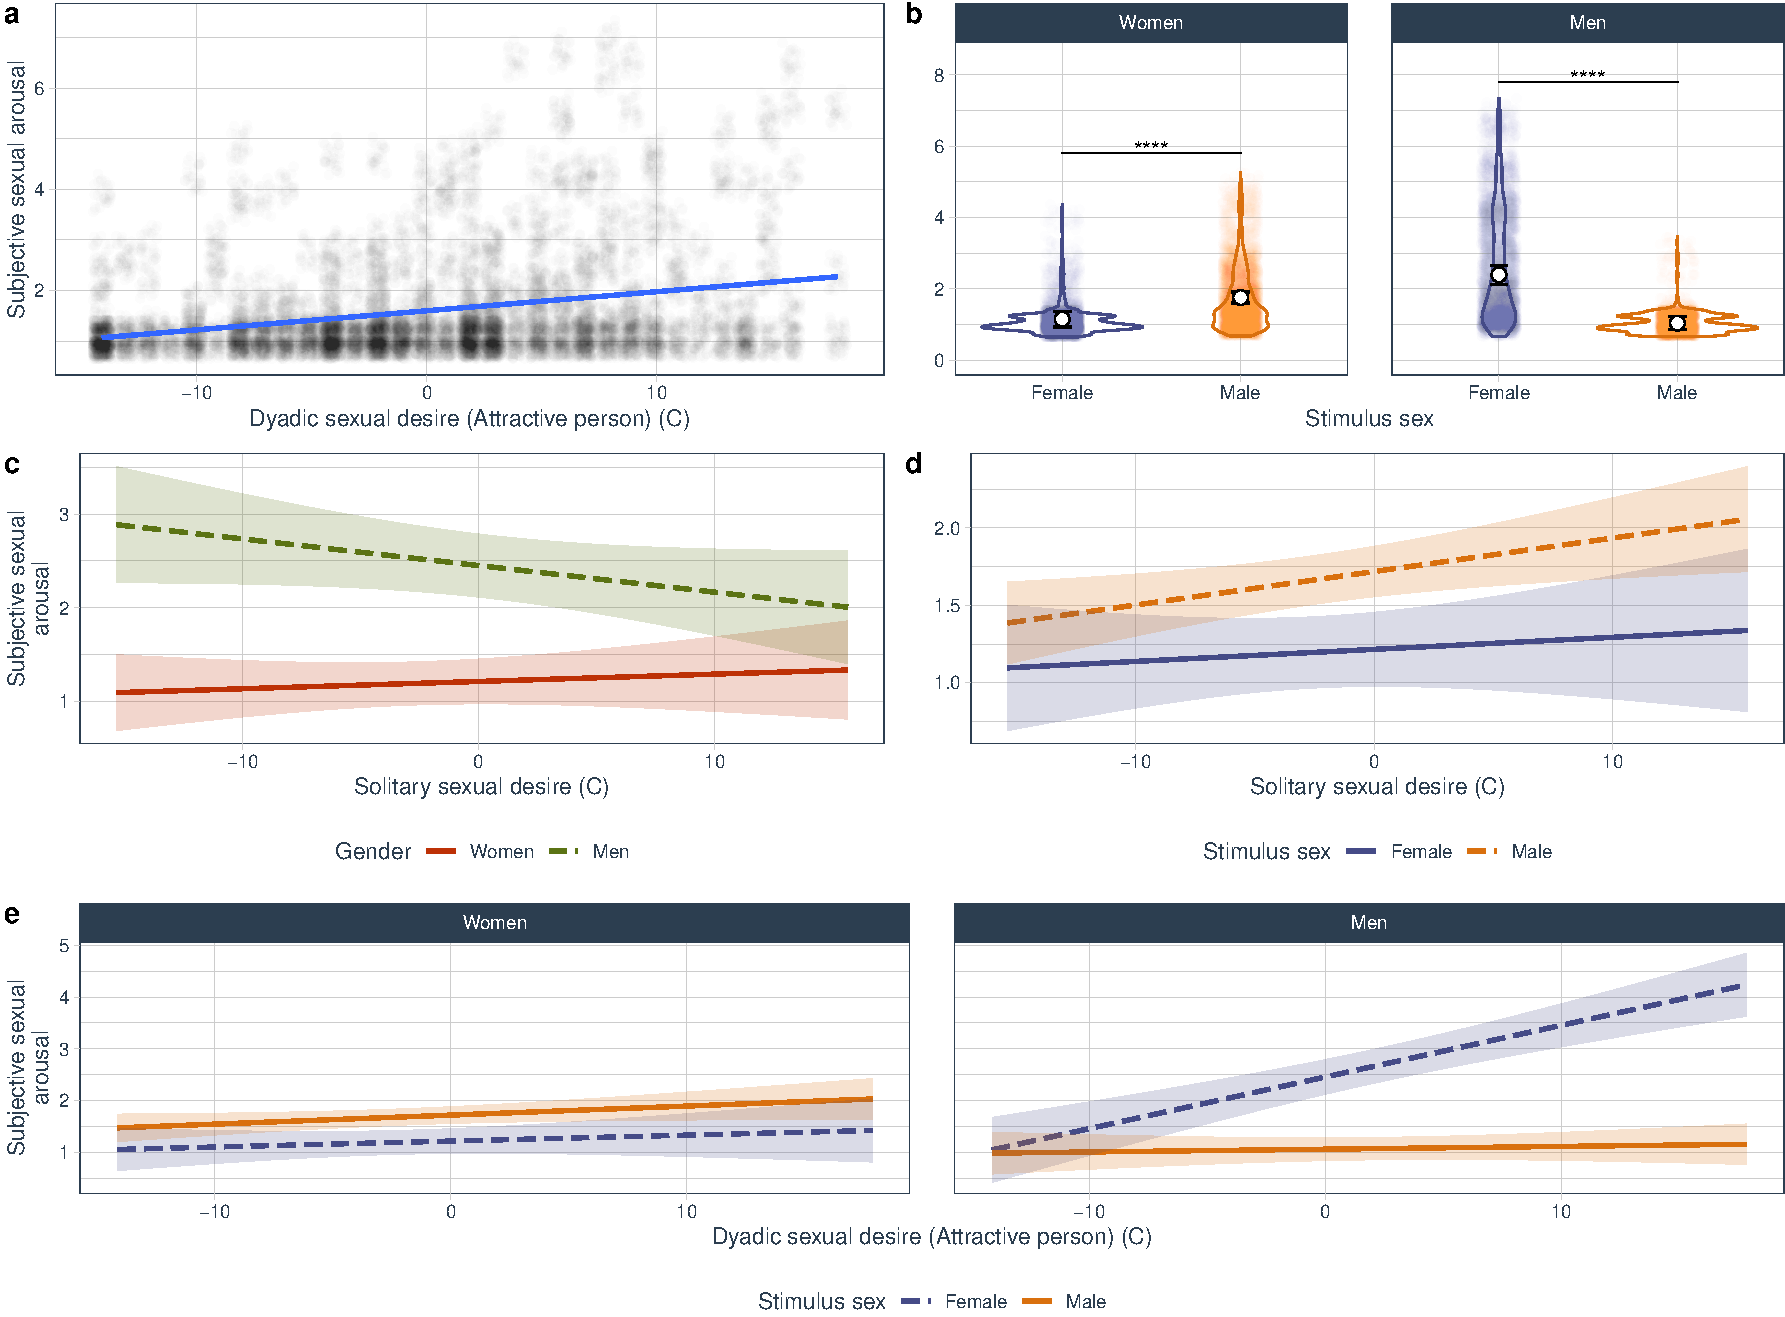
\includegraphics{Deseo_excitacion_sexual_files/figure-latex/fig-h2b-1.pdf}
\caption{\label{fig:fig-h2b}Subjective sexual arousal to non-erotic stimuli: Significant main effects and interactions of model 2B. For detailed results of the model, see Table \ref{tab:tab-m2b}. \textbf{(a)} Main effect of Dyadic sexual desire (Attractive person) on Subjective sexual arousal (for detailed results, see Table \ref{tab:tab-m2b}); \textbf{(b)} interaction between Stimuli sex and gender (significant effects of stimuli sex by participant gender are represented with lines and stars. White dots and black bars represent estimated marginal means and 95\% CI, calculated from 1000 bootstraped simulations; for detailed results, see Table \ref{tab:tab-m2b-emms-b}); \textbf{(c)} interaction between Gender and Solitary sexual desire (for detailed results, see Table \ref{tab:tab-m2b-slo-c}); \textbf{(d)} interaction between Stimuli sex and Solitary sexual desire (for detailed results, see Table \ref{tab:tab-m2b-slo-d}); \textbf{(e)} interaction between Stimuli sex, gender and Dyadic sexual desire (Attractive person) (for detailed results, see Table \ref{tab:tab-m2b-slo-e}). \emph{Women} and \emph{Men} refer to the gender of the participants and \emph{Female} and \emph{Male} to the sex of the stimuli. To better represent the associations between predictor variables and subjective sexual arousal within the model (i.e.~when including all other effects), in all cases the \emph{Y} axis represents values predicted by the model instead of raw values. For statistical significance, *\emph{p} \textless{} 0.05, **\emph{p} \textless{} 0.01, ***\emph{p} \textless{} 0.001, ****\emph{p} \textless{} 0.0001.}
\end{figure}

\hypertarget{session}{%
\section{Session info (for reproducibility)}\label{session}}

\begin{Shaded}
\begin{Highlighting}[]
\FunctionTok{library}\NormalTok{(pander)}
\FunctionTok{pander}\NormalTok{(}\FunctionTok{sessionInfo}\NormalTok{(), }\AttributeTok{locale =} \ConstantTok{FALSE}\NormalTok{)}
\end{Highlighting}
\end{Shaded}

\textbf{R version 4.2.2 (2022-10-31 ucrt)}

\textbf{Platform:} x86\_64-w64-mingw32/x64 (64-bit)

\textbf{attached base packages:}
\emph{stats}, \emph{graphics}, \emph{grDevices}, \emph{utils}, \emph{datasets}, \emph{methods} and \emph{base}

\textbf{other attached packages:}
\emph{pander(v.0.6.5)}, \emph{Hmisc(v.4.7-2)}, \emph{Formula(v.1.2-4)}, \emph{survival(v.3.4-0)}, \emph{lattice(v.0.20-45)}, \emph{berryFunctions(v.1.21.14)}, \emph{rstatix(v.0.7.1)}, \emph{effectsize(v.0.8.2)}, \emph{scales(v.1.2.1)}, \emph{ggpmisc(v.0.5.2)}, \emph{ggpp(v.0.5.0)}, \emph{MetBrewer(v.0.2.0)}, \emph{psych(v.2.2.9)}, \emph{kableExtra(v.1.3.4)}, \emph{performance(v.0.10.2)}, \emph{emmeans(v.1.8.4-1)}, \emph{interactions(v.1.1.5)}, \emph{tidyquant(v.1.0.6)}, \emph{quantmod(v.0.4.20)}, \emph{TTR(v.0.24.3)}, \emph{PerformanceAnalytics(v.2.0.4)}, \emph{xts(v.0.12.2)}, \emph{zoo(v.1.8-11)}, \emph{lubridate(v.1.9.0)}, \emph{timechange(v.0.2.0)}, \emph{ggpubr(v.0.5.0)}, \emph{forcats(v.0.5.2)}, \emph{stringr(v.1.5.0)}, \emph{dplyr(v.1.0.10)}, \emph{purrr(v.1.0.1)}, \emph{readr(v.2.1.3)}, \emph{tidyr(v.1.2.1)}, \emph{tibble(v.3.1.8)}, \emph{ggplot2(v.3.4.0)}, \emph{tidyverse(v.1.3.2)}, \emph{lmerTest(v.3.1-3)}, \emph{lme4(v.1.1-31)}, \emph{Matrix(v.1.5-1)}, \emph{car(v.3.1-1)}, \emph{carData(v.3.0-5)}, \emph{ltm(v.1.2-0)}, \emph{polycor(v.0.8-1)}, \emph{msm(v.1.7)}, \emph{MASS(v.7.3-58.1)}, \emph{readxl(v.1.4.1)} and \emph{knitr(v.1.41)}

\textbf{loaded via a namespace (and not attached):}
\emph{backports(v.1.4.1)}, \emph{jtools(v.2.2.1)}, \emph{systemfonts(v.1.0.4)}, \emph{splines(v.4.2.2)}, \emph{digest(v.0.6.31)}, \emph{htmltools(v.0.5.4)}, \emph{fansi(v.1.0.3)}, \emph{checkmate(v.2.1.0)}, \emph{magrittr(v.2.0.3)}, \emph{cluster(v.2.1.4)}, \emph{googlesheets4(v.1.0.1)}, \emph{see(v.0.7.4)}, \emph{tzdb(v.0.3.0)}, \emph{modelr(v.0.1.10)}, \emph{svglite(v.2.1.1)}, \emph{jpeg(v.0.1-10)}, \emph{colorspace(v.2.0-3)}, \emph{rvest(v.1.0.3)}, \emph{haven(v.2.5.1)}, \emph{xfun(v.0.36)}, \emph{crayon(v.1.5.2)}, \emph{jsonlite(v.1.8.4)}, \emph{glue(v.1.6.2)}, \emph{gtable(v.0.3.1)}, \emph{gargle(v.1.2.1)}, \emph{webshot(v.0.5.4)}, \emph{MatrixModels(v.0.5-1)}, \emph{Quandl(v.2.11.0)}, \emph{abind(v.1.4-5)}, \emph{SparseM(v.1.81)}, \emph{mvtnorm(v.1.1-3)}, \emph{DBI(v.1.1.3)}, \emph{Rcpp(v.1.0.9)}, \emph{htmlTable(v.2.4.1)}, \emph{viridisLite(v.0.4.1)}, \emph{xtable(v.1.8-4)}, \emph{foreign(v.0.8-83)}, \emph{htmlwidgets(v.1.6.1)}, \emph{datawizard(v.0.6.5)}, \emph{httr(v.1.4.4)}, \emph{RColorBrewer(v.1.1-3)}, \emph{ellipsis(v.0.3.2)}, \emph{pkgconfig(v.2.0.3)}, \emph{farver(v.2.1.1)}, \emph{nnet(v.7.3-18)}, \emph{deldir(v.1.0-6)}, \emph{dbplyr(v.2.3.0)}, \emph{utf8(v.1.2.2)}, \emph{tidyselect(v.1.2.0)}, \emph{labeling(v.0.4.2)}, \emph{rlang(v.1.0.6)}, \emph{munsell(v.0.5.0)}, \emph{cellranger(v.1.1.0)}, \emph{tools(v.4.2.2)}, \emph{cli(v.3.6.0)}, \emph{generics(v.0.1.3)}, \emph{broom(v.1.0.2)}, \emph{evaluate(v.0.19)}, \emph{fastmap(v.1.1.0)}, \emph{yaml(v.2.3.6)}, \emph{fs(v.1.5.2)}, \emph{admisc(v.0.30)}, \emph{nlme(v.3.1-160)}, \emph{quantreg(v.5.94)}, \emph{xml2(v.1.3.3)}, \emph{compiler(v.4.2.2)}, \emph{rstudioapi(v.0.14)}, \emph{curl(v.5.0.0)}, \emph{png(v.0.1-8)}, \emph{ggsignif(v.0.6.4)}, \emph{reprex(v.2.0.2)}, \emph{stringi(v.1.7.12)}, \emph{highr(v.0.10)}, \emph{parameters(v.0.20.1)}, \emph{nloptr(v.2.0.3)}, \emph{vctrs(v.0.5.1)}, \emph{pillar(v.1.8.1)}, \emph{lifecycle(v.1.0.3)}, \emph{estimability(v.1.4.1)}, \emph{data.table(v.1.14.6)}, \emph{cowplot(v.1.1.1)}, \emph{insight(v.0.18.8)}, \emph{patchwork(v.1.1.2)}, \emph{R6(v.2.5.1)}, \emph{latticeExtra(v.0.6-30)}, \emph{bookdown(v.0.31)}, \emph{gridExtra(v.2.3)}, \emph{boot(v.1.3-28)}, \emph{assertthat(v.0.2.1)}, \emph{withr(v.2.5.0)}, \emph{mnormt(v.2.1.1)}, \emph{mgcv(v.1.8-41)}, \emph{bayestestR(v.0.13.0)}, \emph{expm(v.0.999-7)}, \emph{parallel(v.4.2.2)}, \emph{hms(v.1.1.2)}, \emph{rpart(v.4.1.19)}, \emph{quadprog(v.1.5-8)}, \emph{grid(v.4.2.2)}, \emph{coda(v.0.19-4)}, \emph{minqa(v.1.2.5)}, \emph{rmarkdown(v.2.19)}, \emph{googledrive(v.2.0.0)}, \emph{numDeriv(v.2016.8-1.1)}, \emph{base64enc(v.0.1-3)} and \emph{interp(v.1.1-3)}

\hypertarget{refs}{%
\section*{Supplementary references}\label{refs}}
\addcontentsline{toc}{section}{Supplementary references}

\hypertarget{refs}{}
\begin{CSLReferences}{1}{0}
\leavevmode\vadjust pre{\hypertarget{ref-barr2013}{}}%
Barr, D. J., Levy, R., Scheepers, C., \& Tily, H. J. (2013). Random effects structure for confirmatory hypothesis testing: {Keep} it maximal. \emph{Journal of Memory and Language}, \emph{68}(3), 255--278. \url{https://doi.org/10.1016/j.jml.2012.11.001}

\leavevmode\vadjust pre{\hypertarget{ref-debruine2021}{}}%
DeBruine, L. M., \& Barr, D. J. (2021). Understanding {Mixed-Effects Models Through Data Simulation}. \emph{Advances in Methods and Practices in Psychological Science}, \emph{4}(1), 2515245920965119. \url{https://doi.org/10.1177/2515245920965119}

\leavevmode\vadjust pre{\hypertarget{ref-fox1992}{}}%
Fox, J., \& Monette, G. (1992). Generalized {Collinearity Diagnostics}. \emph{Journal of the American Statistical Association}, \emph{87}(417), 178--183. \url{https://doi.org/10.1080/01621459.1992.10475190}

\leavevmode\vadjust pre{\hypertarget{ref-kaufmanContrastCodingLeast1974}{}}%
Kaufman, D., \& Sweet, R. (1974). Contrast {Coding} in {Least Squares Regression Analysis}. \emph{American Educational Research Journal}, \emph{11}(4), 359--377. \url{https://doi.org/10.3102/00028312011004359}

\leavevmode\vadjust pre{\hypertarget{ref-keppelDataAnalysisResearch1989}{}}%
Keppel, G., \& Zedeck, S. (1989). \emph{Data analysis for research designs: {Analysis} of variance and multiple regression/correlation approaches}. {W.H. Freeman}.

\leavevmode\vadjust pre{\hypertarget{ref-lmertestcit}{}}%
Kuznetsova, A., Brockhoff, P. B., \& Christensen, R. H. B. (2017). {lmerTest} package: Tests in linear mixed effects models. \emph{Journal of Statistical Software}, \emph{82}(13), 1--26. \url{https://doi.org/10.18637/jss.v082.i13}

\leavevmode\vadjust pre{\hypertarget{ref-emmeanscit}{}}%
Lenth, R. V. (2022). \emph{Emmeans: Estimated marginal means, aka least-squares means}. \url{https://CRAN.R-project.org/package=emmeans}

\leavevmode\vadjust pre{\hypertarget{ref-interactionscit}{}}%
Long, J. A. (2019). \emph{Interactions: Comprehensive, user-friendly toolkit for probing interactions}. \url{https://cran.r-project.org/package=interactions}

\leavevmode\vadjust pre{\hypertarget{ref-ludecke2021}{}}%
Lüdecke, D., Ben-Shachar, M. S., Patil, I., Waggoner, P., \& Makowski, D. (2021). {performance}: An {R} package for assessment, comparison and testing of statistical models. \emph{Journal of Open Source Software}, \emph{6}(60), 3139. \url{https://doi.org/10.21105/joss.03139}

\leavevmode\vadjust pre{\hypertarget{ref-LtmPackageLatent2006}{}}%
Rizopoulos, D. (2006). {ltm}: An {R} package for latent variable modeling and item response theory analyses. \emph{Journal of Statistical Software}, \emph{17}(5), 1--25. \url{https://doi.org/10.18637/jss.v017.i05}

\leavevmode\vadjust pre{\hypertarget{ref-ggplotcit}{}}%
Wickham, H. (2016). \emph{ggplot2: Elegant graphics for data analysis}. Springer-Verlag New York. \url{https://ggplot2.tidyverse.org}

\leavevmode\vadjust pre{\hypertarget{ref-tidyversecit}{}}%
Wickham, H., Averick, M., Bryan, J., Chang, W., McGowan, L. D., François, R., Grolemund, G., Hayes, A., Henry, L., Hester, J., Kuhn, M., Pedersen, T. L., Miller, E., Bache, S. M., Müller, K., Ooms, J., Robinson, D., Seidel, D. P., Spinu, V., \ldots{} Yutani, H. (2019). Welcome to the {tidyverse}. \emph{Journal of Open Source Software}, \emph{4}(43), 1686. \url{https://doi.org/10.21105/joss.01686}

\leavevmode\vadjust pre{\hypertarget{ref-dplyrcit}{}}%
Wickham, H., François, R., Henry, L., \& Müller, K. (2022). \emph{Dplyr: A grammar of data manipulation}. \url{https://CRAN.R-project.org/package=dplyr}

\leavevmode\vadjust pre{\hypertarget{ref-osfrcit}{}}%
Wolen, A. R., Hartgerink, C. H. J., Hafen, R., Richards, B. G., Soderberg, C. K., \& York, T. P. (2020). {osfr}: An {R} interface to the open science framework. \emph{Journal of Open Source Software}, \emph{5}(46), 2071. \url{https://doi.org/10.21105/joss.02071}

\leavevmode\vadjust pre{\hypertarget{ref-knitrcit}{}}%
Xie, Y. (2014). Knitr: A comprehensive tool for reproducible research in {R}. In V. Stodden, F. Leisch, \& R. D. Peng (Eds.), \emph{Implementing reproducible computational research}. {Chapman and Hall/CRC}. \url{https://doi.org/10.1201/9781315373461-1}

\leavevmode\vadjust pre{\hypertarget{ref-kableExtracit}{}}%
Zhu, H. (2020). \emph{kableExtra: Construct complex table with 'kable' and pipe syntax}. \url{https://CRAN.R-project.org/package=kableExtra}

\end{CSLReferences}

\end{document}
